\documentclass[12pt]{book}
\usepackage{amsmath}
\usepackage{bm}
\usepackage{colortbl}
\usepackage{graphicx}
\usepackage{caption}
\usepackage{fullpage}
\usepackage{afterpage}
\usepackage{float}
\usepackage{multirow}
\usepackage[nodisplayskipstretch]{setspace}
\usepackage{booktabs}
\usepackage{textcomp}
\usepackage{gensymb}
\usepackage[utf8]{inputenc} 
%\usepackage{parskip}
\usepackage{xr}
\usepackage{pdflscape}
\usepackage[labelfont=bf,tableposition=top]{caption}
\usepackage[inline]{enumitem}
\usepackage{wrapfig}
\usepackage{longtable}
\usepackage{subfig}
\usepackage[hidelinks]{hyperref}
\usepackage{geometry}
\usepackage{fancyhdr}
\usepackage[acronym,nomain,toc,makeindex ]{glossaries}
\usepackage{graphicx}
\usepackage{cleveref} %This need to be the last package for it to work properly 
\usepackage[hyperref=true,maxcitenames=3,maxbibnames=3,url=false,isbn=false,backref=true,natbib=true,backend=biber,sorting=nyvt,defernumbers=false, style=authoryear]{biblatex}


%
%
%	TITLE PAGE DEFINITION
%
%
\title{Genetic and Environmental risk factors of Schizophrenia and Autism}
\date{\today}
\author{\href{mailto:choishingwan@gmail.com}{Choi Shing Wan}\\
	
\includegraphics[width=0.5\textwidth]{hkuLogo.jpg}}
\singlespacing
\renewcommand*\contentsname{Contents}

\newcommand{\rom}[1]{\uppercase\expandafter{\romannumeral #1\relax}}
\newcommand*{\glng}{\glsentrylong}
\newcommand*{\Glng}{\Glsentrylong}
\newcommand{\beginsupplement}{%
	\setcounter{table}{0}
	\renewcommand{\thetable}{S\arabic{table}}%
	\setcounter{figure}{0}
	\renewcommand{\thefigure}{S\arabic{figure}}%
}
\newcommand{\specialcell}[2][c]{\begin{tabular}[#1]{@{}c@{}}#2\end{tabular}}

%
%	GLOSSARY SECTION
%
\addbibresource[datatype=bibtex]{citation/citation.bib}
\makeglossary
\newacronym{scz}{SCZ}{schizophrenia}
\newacronym[longplural={Genome Wide Association Studies}]{GWAS}{GWAS}{Genome Wide Association Study}
\newacronym{wgs}{WGS}{Whole Genome Sequencing}
\newacronym{SNP}{SNP}{Single Nucleotide Polymorphism}
\newacronym{LD}{LD}{Linkage Disequilibrium}
\newacronym{PGS}{PGS}{Polygenic Risk Score}
\newacronym{tSVD}{tSVD}{Truncated Singular Value Decomposition}
\newacronym{SVD}{SVD}{Singular Value Decomposition}
\newacronym{shrek}{SHREK}{SNP Heritability and Risk Estimation Kit}
\newacronym{gcta}{GCTA}{Genome-wide Complex Trait Analysis}
\newacronym{ldsc}{LDSC}{LD SCore}
\newacronym{CEU}{CEU}{Northern Europeans from Utah}
\newacronym{se}{SE}{standard error}
\newacronym{maf}{maf}{Minor Allele Frequency}
\newacronym{isc}{ISC}{International Schizophrenia Consortium}
\newacronym{mgs}{MGS}{Molecular Genetic of Schizophrenia}
\newacronym{sgene}{SGENE}{Schizophrenia Genetics Consortium}
\newacronym{pgc}{PGC}{Psychiatric Genomics Consortium}
\newacronym{rin}{RIN}{RNA integrity number}
\newacronym{gd}{GD}{Gestation Day}
\newacronym{rpkm}{RPKM}{Reads Per Kilobase per Million mapped reads}
\newacronym{wgcna}{WGCNA}{Weighted Gene Co-expression Network Analysis}
\newacronym{pc}{PC}{Principle Component}
\newacronym{GO}{GO}{Gene Ontology}
\newacronym{MAGMA}{MAGMA}{Multi-marker Analysis of GenoMic Annotation}
\newacronym{ngs}{NGS}{next generation sequencing}
\newacronym{dsm}{DSM}{Diagnostic and Statistical Manual of Mental Disorders}
\newacronym{mse}{MSE}{mean squared error}
\newacronym{who}{WHO}{World Health Organization}
\newacronym{yld}{YLD}{years lost due to disability}
\newacronym{ci}{CI}{confidence interval}
\newacronym{iq}{IQ}{intelligence quotient}
\newacronym{polyic}{PolyI:C}{polyriboinosinic-polyribocytidilic acid}
\newacronym{lps}{LPS}{lipopolysaccharide}
\newacronym{il6}{IL-6}{Interleukin-6}
\newacronym{mz}{MZ}{monozygotic}
\newacronym{dz}{DZ}{dizygotic}
\newacronym{mia}{MIA}{maternal immune activation}
\newacronym{ncp}{NCP}{non-centrality parameter}
\newacronym{cnv}{CNV}{copy number variation}
\newacronym{grm}{GRM}{Genetic Relationship Matrix}
\newacronym{gc}{GC}{Genomic Control}
\newacronym{mhc}{MHC}{major histocompatibility complex}
\newacronym{cns}{CNS}{central nervous system}
\newacronym{panss}{PANSS}{Positive and Negative Symptom Scale}
\newacronym{fga}{FGA}{First Generation Antipsychotic}
\newacronym{sga}{SGA}{Second Generation Antipsychotic}
\newacronym{nmda}{NMDA}{N-methyl-D-aspartate}
\newacronym{eps}{EPS}{extrapyramidal motor symptoms}
\newacronym{td}{TD}{Tardive dyskinesia}
\newacronym{pet}{PET}{positron emission tomography}
\newacronym{catie}{CATIE}{Clinical Antipsychotic Trials of Intervention Effectiveness}
\newacronym{pca}{PCA}{principle component analysis}
\newacronym{fdr}{FDR}{false discovery rate}
%
%
%	FORMATING SECTION
%
%

\pagestyle{fancy}
\fancyhf{}
\fancyfoot[LE,RO]{\thepage}
\renewcommand{\footrulewidth}{1pt}
\fancyhead[LE]{\leftmark}
\fancyhead[RO]{\rightmark}

\geometry{
	top=1in,            % <-- you want to adjust this
	inner=1in,
	outer=1in,
	bottom=1in,
	headheight=3ex,       % <-- and this
	headsep=2ex,          % <-- and this
}


\raggedbottom %Remove it before printing as this is something to do with global settings. Can make each page look uneven but more dense. 
\onehalfspacing
%\doublespacing
%\includeonly{heritability_estimation}
\includeonly{literature_review}

\makeindex
\begin{document}\thispagestyle{empty}
\pagestyle{empty}

%\maketitle
\begin{titlepage}
	\begin{center}
		\vspace*{1cm}
		
		\Huge
		\textbf{Heritability Estimation and Risk Prediction in Schizophrenia}
		
		\vspace{0.5cm}
		\LARGE
		
		\vspace{1.5cm}
		
		\textbf{\href{mailto:choishingwan@gmail.com}{Choi Shing Wan}}
		
		\vfill
		
		A thesis submitted in partial fulfillment of the requirements for \\
		the Degree of Doctor of Philosophy
		
		\vspace{0.8cm}
		
		
\includegraphics[width=0.4\textwidth]{figure/hkuLogo.jpg}
		
		\Large
		Department of Psychiatry\\
		University of Hong Kong\\
		Hong Kong\\
		\today
		
	\end{center}
\end{titlepage}


\frontmatter 

	\cleardoublepage
	\phantomsection
	\addcontentsline{toc}{chapter}{Declaration}
	\newgeometry{inner=2in, outer=2in}
	\chapter*{\centerline{Declaration}}
	\vspace{1cm}
	I declare that this thesis represents my own work, except where due acknowledgments	is made, and that it has not been previously included in a thesis, dissertation or report submitted to this University or to any other institution for a degree,	diploma or other qualification.
	\vspace{1.5cm}
	
	\centerline{Signed....................................................................}
	\restoregeometry
	\cleardoublepage
	\phantomsection
	\addcontentsline{toc}{chapter}{Acknowledgments}
	\chapter*{\centerline{Acknowledgements}}
	\cleardoublepage
	\phantomsection
	\begin{singlespace}
	\printglossary[title=Abbreviations,toctitle=Abbreviations]
	\cleardoublepage
	\phantomsection
	%To generate the correct abbreviations, use alt+shift+F1 twice before using F1
	
	\cleardoublepage
	\phantomsection
	\addcontentsline{toc}{chapter}{Contents}
		\tableofcontents
		\listoffigures
		\listoftables
	\end{singlespace}
\mainmatter
\pagestyle{fancy}

\setlength{\parindent}{4em}
\setlength{\parskip}{0.75em}
	
		\chapter{Introduction}
	% Disease background
	\section{Schizophrenia}
	\Glng{scz} is a devastating psychiatric disorder affecting approximately 0.3--0.7\% of the population worldwide \citep{AmericanPsychiatricAssociation2013}.
	According to the \gls{dsm}-\rom{5}, which is one of the standard diagnostic tools in psychiatry, a diagnosis of \glng{scz} (F20.9) can only be reached if the patient has suffered from 2 or more of the following symptoms for a significant portion of time during a 1-month period: 
	\begin{enumerate*}[label=\arabic*\upshape)]
		\item delusion; \label{ls:delusion}
		\item hallucination;\label{ls:hallucinations}
		\item disorganized speech;\label{ls:disorganizedSpeech}
		\item grossly disorganized or catatonic behaviour; and\label{ls:catatonicBehavior}
		\item negative symptoms such as diminished emotional expression,\label{ls:negativeSymptoms}
	\end{enumerate*}  where one of the symptom must be either (\ref{ls:delusion}, (\ref{ls:hallucinations} or (\ref{ls:disorganizedSpeech}, which are known as positive symptoms.
	Signs of disturbance need to persist for at least 6-month before the patient can be diagnosed with \glng{scz}.
	Current medical treatment of \glng{scz}, based on dopamine D2 receptor blockage, is effective only for the amelioration of positive symptoms in approximately 2/3 of patients.
	
	Because of its disabling symptoms and the lack of entirely effective treatments, \glng{scz} imposes a serious and long lasting health, social and financial burden to patients and their families \citep{Knapp2004}. 
	\Glng{scz} patients also have an increased tendency to commit suicide \citep{Saha2007}.
	Based on an \gls{who} report, \glng{scz} was one of the top 20 leading cause of \gls{yld} in 2012, ranking 16 among all possible causes (\cref{tab:whoYLD}).
	\begin{table}[ht]
		\centering
		\caption[Top 20 leading causes of \glng{yld}]{Top 20 leading causes of \gls{yld} calculated by \gls{who} in year 2012.
			\Glng{scz} was considered as one of the top 20 leading causes of \gls{yld} \citep{Geneva2013}.}
		\begin{tabular}{rp{5cm}rrr}
			\toprule
			Rank  & Cause & \gls{yld} (000s) & \% \gls{yld} & \specialcell[b]{\gls{yld} per \\100k population}\\
			\midrule
			0     & All Causes & 740,545 & 100   & 10466 \\
			1     & Unipolar depressive disorders & 76,419 & 10.3  & 1080 \\
			2     & Back and neck pain & 53,855 & 7.3   & 761 \\
			3     & Iron-deficiency anaemia & 43,615 & 5.9   & 616 \\
			4     & Chronic obstructive pulmonary disease & 30,749 & 4.2   & 435 \\
			5     & Alcohol use disorders & 27,905 & 3.8   & 394 \\
			6     & Anxiety disorders & 27,549 & 3.7   & 389 \\
			7     & Diabetes mellitus & 22,492 & 3     & 318 \\
			8     & Other hearing loss & 22,076 & 3     & 312 \\
			9     & Falls & 20,409 & 2.8   & 288 \\
			10    & Migraine & 18,538 & 2.5   & 262 \\
			11    & Osteoarthritis & 18,096 & 2.4   & 256 \\
			12    & Skin diseases & 15,744 & 2.1   & 223 \\
			13    & Asthma & 14,134 & 1.9   & 200 \\
			14    & Road injury & 13,902 & 1.9   & 196 \\
			15    & Refractive errors & 13,498 & 1.8   & 191 \\
			16    & Schizophrenia & 13,408 & 1.8   & 189 \\
			17    & Bipolar disorder & 13,271 & 1.8   & 188 \\
			18    & Drug use disorders & 10,620 & 1.4   & 150 \\
			19    & Endocrine, blood, immune disorders & 10,495 & 1.4   & 148 \\
			20    & Gynecological diseases & 10,227 & 1.4   & 145 \\
			\bottomrule
		\end{tabular}%
		\label{tab:whoYLD}%
	\end{table}%
	In view of its severity, \glng{scz} has drawn much attention from the research community to delineate disease etiology and mechanisms, and identify risk factors associated with \glng{scz}.
	Ultimately, the goal of \glng{scz} research is to identify effective treatment(s) to improve the quality of life of patients.
	
	\section{Understanding Disease Etiology}
	An important first step in \glng{scz} research is to understand whether if genetic or environmental variation contribute more to the disease etiology.
	A measure of the relative contribution of genetic and environmental influences to individual differences in the liability to a disorder is \emph{heritability}.
	There are two definitions of heritability: the broad sense heritability and the narrow sense heritability.
	Broad sense heritability is defined as the \emph{proportion} of total variance of a trait in a population explained by the \emph{total} variation of genetic factors in the population, whereas the narrow sense heritability only takes into account of the variation of \emph{additive} genetic factors in the population instead of the total variation of genetic factors.
	
	\subsection{Broad Sense Heritability}
	For any phenotype, one can partition it into a combination of genetic and environmental components \citep{Falconer1996}
	$$
	\text{Phenotype (P)}=\text{Genotype (G)}+\text{Environment (E)}
	$$
	In the absence of gene-environmental correlation or interaction, the variance of the observed phenotype ($\sigma_P^2$) can be expressed as the sum of the variance of genotype ($\sigma_G^2$) and variance of environment ($\sigma_E^2$)
	$$
	\sigma_P^2=\sigma_G^2+\sigma_E^2
	$$
	The ratio between the variance of the observed phenotype and the variance of the genetic effects is then defined as the broad sense heritability:
	$$
	H^2=\frac{\sigma_G^2}{\sigma_P^2}
	$$
	
	One key feature of heritability is that it is a \emph{ratio} of \emph{population} measurements at a specific time point.
	As a result, the heritability of a trait can differ in different strata of the same population (because of differences in the environment), and in different populations (because of differences in both genes and environment).
	A classic example is \gls{iq}, which increases in heritability with increasing age \citep{Bouchard2013}.
	It was hypothesized that the shared environment has a relatively larger effect on individuals when they were young, and gradually diminishes when they grow older and become more independent.
	The reduction in shared environmental influences results in an \emph{increased portion} of variance in \gls{iq} explained by genetic differences \citep{Bouchard2013}. 
	
	The definition of heritability becomes more complicated when we take into account different forms of genetic effects; this leads to the concept of narrow sense heritability.
	
	\subsection{Narrow Sense Heritability}
	The effects of genes are not always additive but can differ depending on the other gene at the same locus (dominance) or genes at different loci (epistasis).
	As a result, one can partition the total genetic variance into variance due to additive genetic effects ($\sigma_A^2$), variance due to dominant genetic effects ($\sigma_D^2$), and variance due to other epistatic genetic effects ($\sigma_I^2$), as follows:
	$$
	\sigma_G^2=\sigma_A^2+\sigma_D^2+\sigma_I^2
	$$
	
	As individuals only transmit one copy of each gene at a single genetic locus to their offspring, relatives other than full siblings and identical twins will only share a maximum of one gene for each locus.
	Considering that dominance and epistatic genetic effects are interactive effect, which usually involve more than one gene, these effects are unlikely to contribute substantially to the resemblance between relatives other than monozygotic twins and full siblings \citep{Visscher2008}.
	On the other hand, the additive genetic effects are usually transmitted from parent to offspring, thus it is more useful to consider the narrow sense heritability ($h^2$) which only includes the additive genetic effects, when predicting parent-offspring resemblance:
	\begin{align}
	h^2&=\frac{\sigma_A^2}{\sigma_P^2} \notag\\
	h^2&=\frac{\sigma_A^2}{\sigma_G^2+\sigma_E^2}
	\label{eq:narrowHeritability}
	\end{align}
	
	To obtain the additive genetic effect, we can first consider the genetic effect of a parent to be $G_p=A+D$. 
	As only half of the additive effect were transmitted to their offspring, the child will have a genetic effect of $G_c=\frac{1}{2}A+\frac{1}{2}A'+D'$ where $A'$ is the additive genetic effect obtained from another parent by random and $D'$ is the non-additive genetic effect in the offspring.
	If we then consider the parent offspring covariance, we will get
	\begin{align}
	\mathrm{Cov_{OP}}&= \sum(\frac{1}{2}A+\frac{1}{2}A'+D')(A+D)\notag\\
	&=\frac{1}{2}\sum A^2+\frac{1}{2}\sum AD + \frac{1}{2}\sum A'(A+D) +D'(A+D) \notag\\ 
	&=\frac{1}{2}V_A+ \frac{1}{2}\mathrm{Cov}_{AD} + \frac{1}{2}\mathrm{Cov}_{A'A} + \frac{1}{2}\mathrm{Cov}_{A'D} +\mathrm{Cov}_{D'A} +\mathrm{Cov}_{D'D}  
	\label{eq:halfCompletedCovOP}
	\end{align} 
	Under the assumption of random mating,  $A'$ should be independent from $A$ and $D$. 
	Moreover, as $D'$ was specific to the child, it should be independent from $A$ and $D$, with the covariance between the additive genetics and non-additive genetics being zero \citep{Falconer1996}.
	Thus, \cref{eq:halfCompletedCovOP} becomes
	\begin{align}
	\mathrm{Cov_{OP}} &= \frac{1}{2}V_A+\mathrm{Cov}_{AD} \notag\\
	&= \frac{1}{2}V_A
	\label{eq:covOP}
	\end{align}
	Now if we assume the variance of phenotype of the parent and offspring were the same, then using \cref{eq:covOP}, we can obtain the narrow-sense heritability as
	\begin{align}
	h^2 &= \frac{1}{2}\frac{V_A}{\sigma_P^2}
	\label{eq:narrowHerit}
	\end{align}

	In the simple linear regression equation $Y=X\beta+\epsilon$, the regression slope can be calculated as 
	\begin{equation}
	\beta_{XY} = \frac{\mathrm{Cov}_{XY}}{\sigma_{X}{Y}}
	\end{equation}
	which resemble \cref{eq:narrowHerit}. 
	Therefore,  we can calculate the narrow sense heritability as
	\begin{equation}
	h^2 = 2\beta_{OP}
	\label{eq:narrowSenseHerit}
	\end{equation}
	where $\beta_{OP}$ is the slope of the simple linear regression regressing the phenotype of an offspring to the phenotype of \emph{one} of its parents.
	We can further generalize \cref{eq:narrowSenseHerit} to all possible relativeness 
	\begin{equation}
	h^2=\frac{\beta_{XY}}{r}
	\label{eq:finalNarrow}
	\end{equation}
	where $r$ is the relativeness of $X$ and $Y$.
	
	A key assumption in this calculation is that only additive genetic factors are shared among relatives.
	However, this is very unlikely to be entirely true as relatives do tends to be in the same cultural group and might have similar socio-economic status.
	These might all contribute to the variance of the trait, thus lead to bias in \cref{eq:finalNarrow} and we shall discuss the partitioning of variance in the later sections.
	
	Nonetheless, \cref{eq:finalNarrow} provide a simple example to the calculation of the narrow sense heritability.
	However, in the case of discontinuous trait (e.g. disease status) the calculation becomes more complicated because the variance of the phenotype was dependent on the population prevalence.
	As \cref{eq:finalNarrow} does not account for the trait prevalence, it cannot be directly applied to discontinuous traits.
	In order to perform heritability estimation on discontinuous trait, the concept of liability threshold model proposed by \cite{Falconer1965} is necessary with the calculation.
	
	\subsection{Liability Threshold}
	\label{sec:liability}
	According to the central limit theorem, if a phenotype is determined by a multitude of genetics and environmental factors with relatively small effect, then its distribution will likely follow a normal distribution as is the case of many quantitative traits \citep{Visscher2008}. % No, what if there is interaction between variables? Then it will break the CLT
	The variance of phenotype can therefore be calculated as the variance under the normal distribution.
	However, such is not the case for disease like \glng{scz} where only a dichotomous disease status (``affected'' and ``normal'') are obtained.
	The variance of these phenotypes are therefore more difficult to obtain.
	
	\citet{Falconer1965} proposed the liability threshold model, which suggests that these discontinuous traits also follow a continuous distribution with an additional parameter called the ``liability threshold''.
	Under the liability threshold model, the discontinuous traits are assumed to be affected by combination of multitude of genetics and environmental factors, each with small effects.
	The main difference is that the phenotype of an individual is determined by whether if the combined effects of these factors (``liability'') are above a particular threshold (``liability threshold'') (\cref{fig:liability}), e.g. only when an individual has a liability above the liability threshold will he/she be affected.
	\begin{figure}
		\centering
		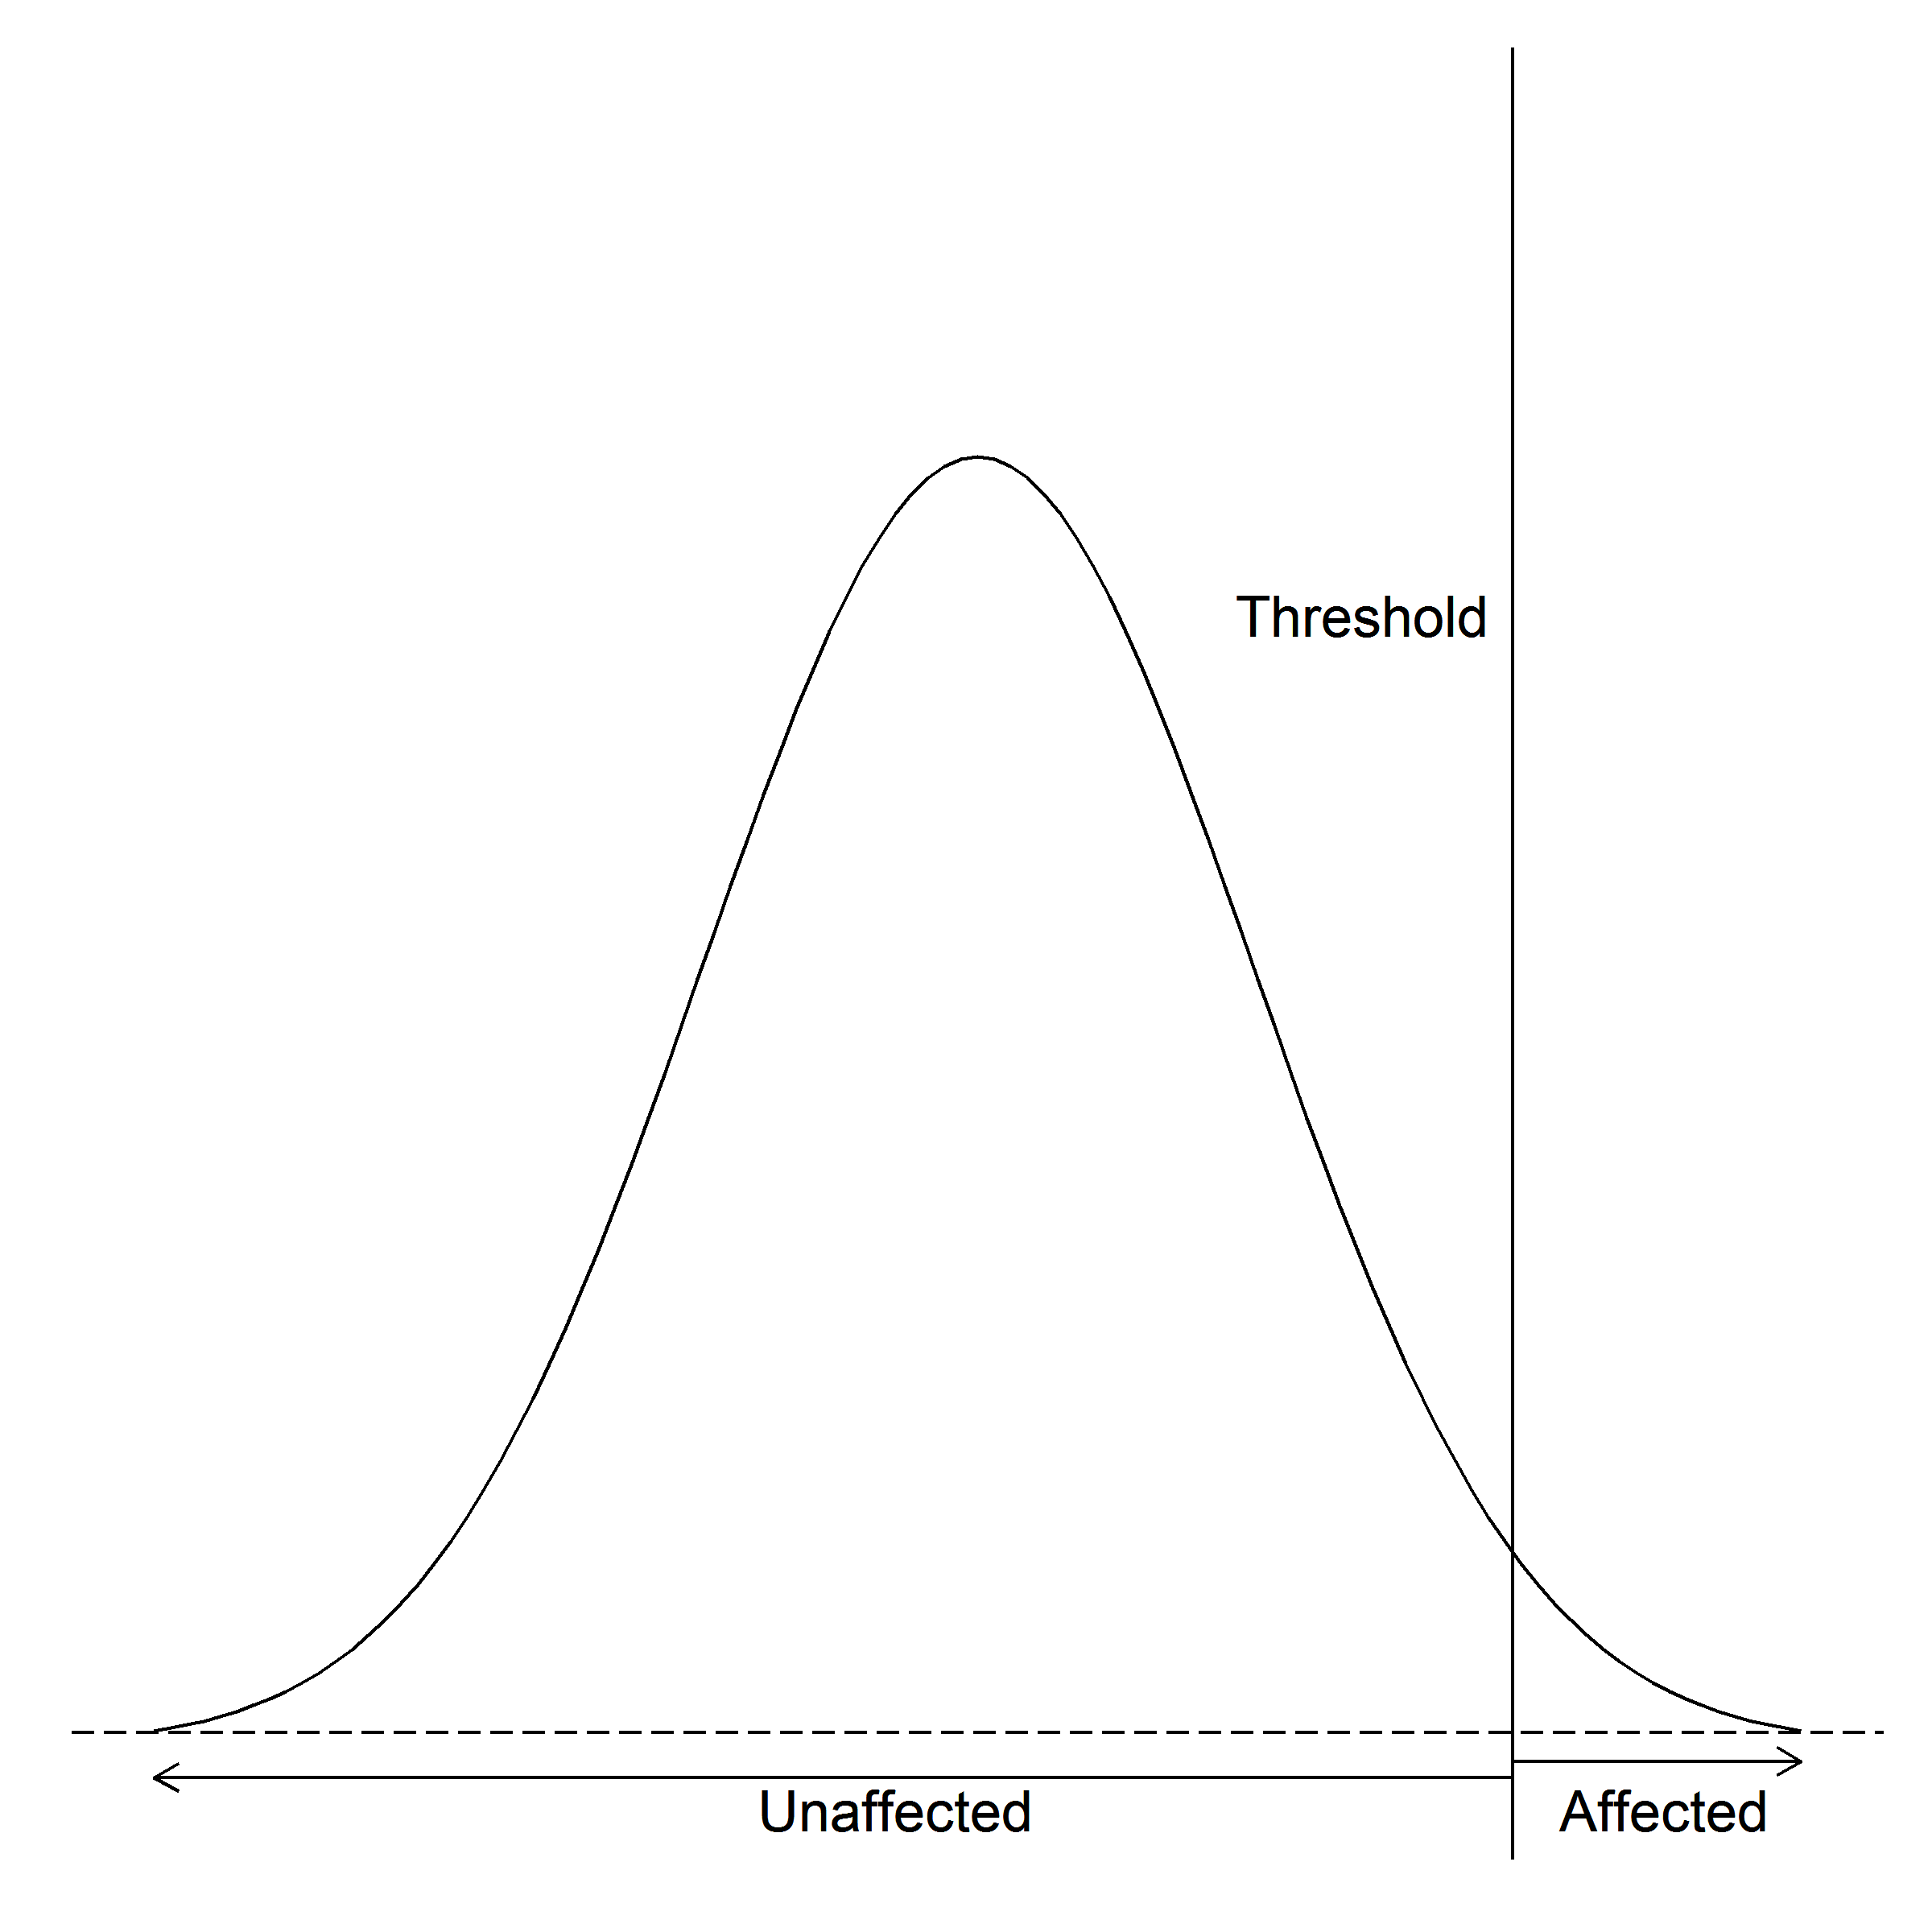
\includegraphics[width=0.5\textwidth]{figure/liability.png}
		\caption[Liability Threshold Model]{
			The liability threshold model.
			Only when an individual has a liability above the liability threshold will he/she be affected.
			}
			\label{fig:liability}
	\end{figure}
	One can then estimate the heritability of the discontinuous trait by comparing the mean liability of the general population when compared to the relatives of the affected individuals.	
	For example, if we consider a single threshold model of a dichotomous trait, where 
	\begin{align}
	T_G &= \text{Liability threshold of the general population}\notag\\
	T_R &= \text{Liability threshold of relatives of the index case} \notag\\
	q_G &= \text{Prevalence in the general population}\notag\\
	q_R &= \text{Prevalence in relatives of the index case}\notag\\
	L_a &= \text{Mean Liability of the index case} \notag
	\end{align}
	by assuming both the liability distribution of the general population and the relative of the index case both follows the standard normal distribution, we can align the two distributions with respect to $T_G$ and $T_R$. 
	We can then calculate the mean liability of the index case $L_a$ as $L_a=\frac{z_G}{q_G}$ where $z_G$ is the density of the normal distribution at the liability threshold $T_G$.
	Then we can express the regression of relatives' liability on the liability of the index case as
	\begin{align}
	\beta &= \frac{T_G-T_R}{L_a}
	\label{eq:liability}
	\end{align}
	
	Thus, by applying \cref{eq:liability} to \cref{eq:finalNarrow}, we get
	\begin{align}
	h^2 =\frac{T_G-T_R}{rL_a}
	\end{align}
	
	\subsection{Adoption Study}
	% Need to go deeper into twin studies
	One key limitation of \cref{eq:finalNarrow} is its inability to discriminate the genetic factors from the shared environmental factors.
	Relatives can share not only their additive genetic effect of alleles, they also share some of the environmental factors such as diet and socio-economic status. 
	
	In order to discriminate the genetic factors from the shared environmental factors, adoption study can be carried out. 
	An advantage of adoption studies is that if the child was separated from their family early after birth, then the shared environmental factors should be minimized.
	Any resemblance between the parent and child should be driven mainly by the shared genetic factors.
	
	
	In the classical adoption study carried out by \citet{HESTON1966} in 1966, 47 individuals who were born to schizophrenic mothers during the period from 1915 to 1947 were collected. 
	The child were separated from their mother within three days of birth and sent to a foster family. 
	50 matched controls were also recruited in this study.
	It was observed that there was an increased risk of \glng{scz} in individuals born to schizophrenic mothers when compared to the control groups even-though they were brought up in a different environment as that of their mother.
	This provide strong support for \glng{scz} as a genetic disorder. 
%	This result suggested that \glng{scz} is likely driven by the shared genetic factors instead of the shared environmental factors.
	
	\subsection{Twin Studies}
	Despite the usefulness of adoption studies, collection of adoption data are extremely difficult. 
	Moreover, any prenatal influence such as alcohol abuse and malnutrition during pregnancy can confound the results.
	Therefore, an alternative method would be the twin studies, utilizing the genetic relationship between \gls{mz} and \gls{dz} twins.
	
	\gls{mz} twins share all their genetic components (both additive ($A$) and non-additive ($D$) genetic factors) and common environmental factors ($C$).
	The only difference between the \gls{mz} twins is the non-shared environmental factors ($E$).
	For \gls{dz} twins, they share the same common environmental factors.
	However, only $\frac{1}{2}$ of their additive genetic factors and $\frac{1}{4}$ of their non-additive genetic factors are shared, whereas none of the non-shared environmental factors are shared among the twins \citep{Rijsdijk2002}.
	
	In view of this, \cite{Falconer1996} derived the heritability as
	\begin{equation}
	h^2 = 2(\rho_{MZ}-\rho_{DZ})
	\end{equation}
	where $\rho_{MZ}$ and $\rho_{DZ}$ are the phenotype correlation between the \gls{mz} twins and \gls{dz} twins respectively.
	
	By combining Falconer's formula and the concept of liability threshold model, \citet{Gottesman1967} estimated that the heritability of \glng{scz} to be $>60\%$ based on previously collected twin data.
	This provides strong evidence that the genetic variation contributes more to the variance of \glng{scz}.
	
	The result was further supported by one of the landmark meta-analysis study conducted by \citet{Sullivan2003}.
	Based on data obtained from 12 published \glng{scz} twin studies, \citet{Sullivan2003} found a much contribution from genetics on the liability of \glng{scz} ($81\%$, \gls{ci}=$73\%-90\%$).
	Furthermore, in the large scale population based studies peroformed by \citet{Lichtenstein2009}, the genetic contribution to \glng{scz} was found to be $64\%$.
	Together, these results provide strong support for \glng{scz} as a genetic disorder. 
	
	\section{Schizophrenia Genetics}
	Although \glng{scz} is highly heritable, little is known about the disease mechanism of \glng{scz} and the genetic architecture of the disorder. 
	However, it was observed that the lifetime morbid risk of \gls{mz} twins were only $48\%$ (\cref{fig:lifeMRscz}), suggesting that it is unlikely for \glng{scz} to follow the Mendelian framework \citep{Gottesman1967,Gottesman1982,gottesman1991schizophrenia}.
	
	\begin{figure}[t]
		\centering
		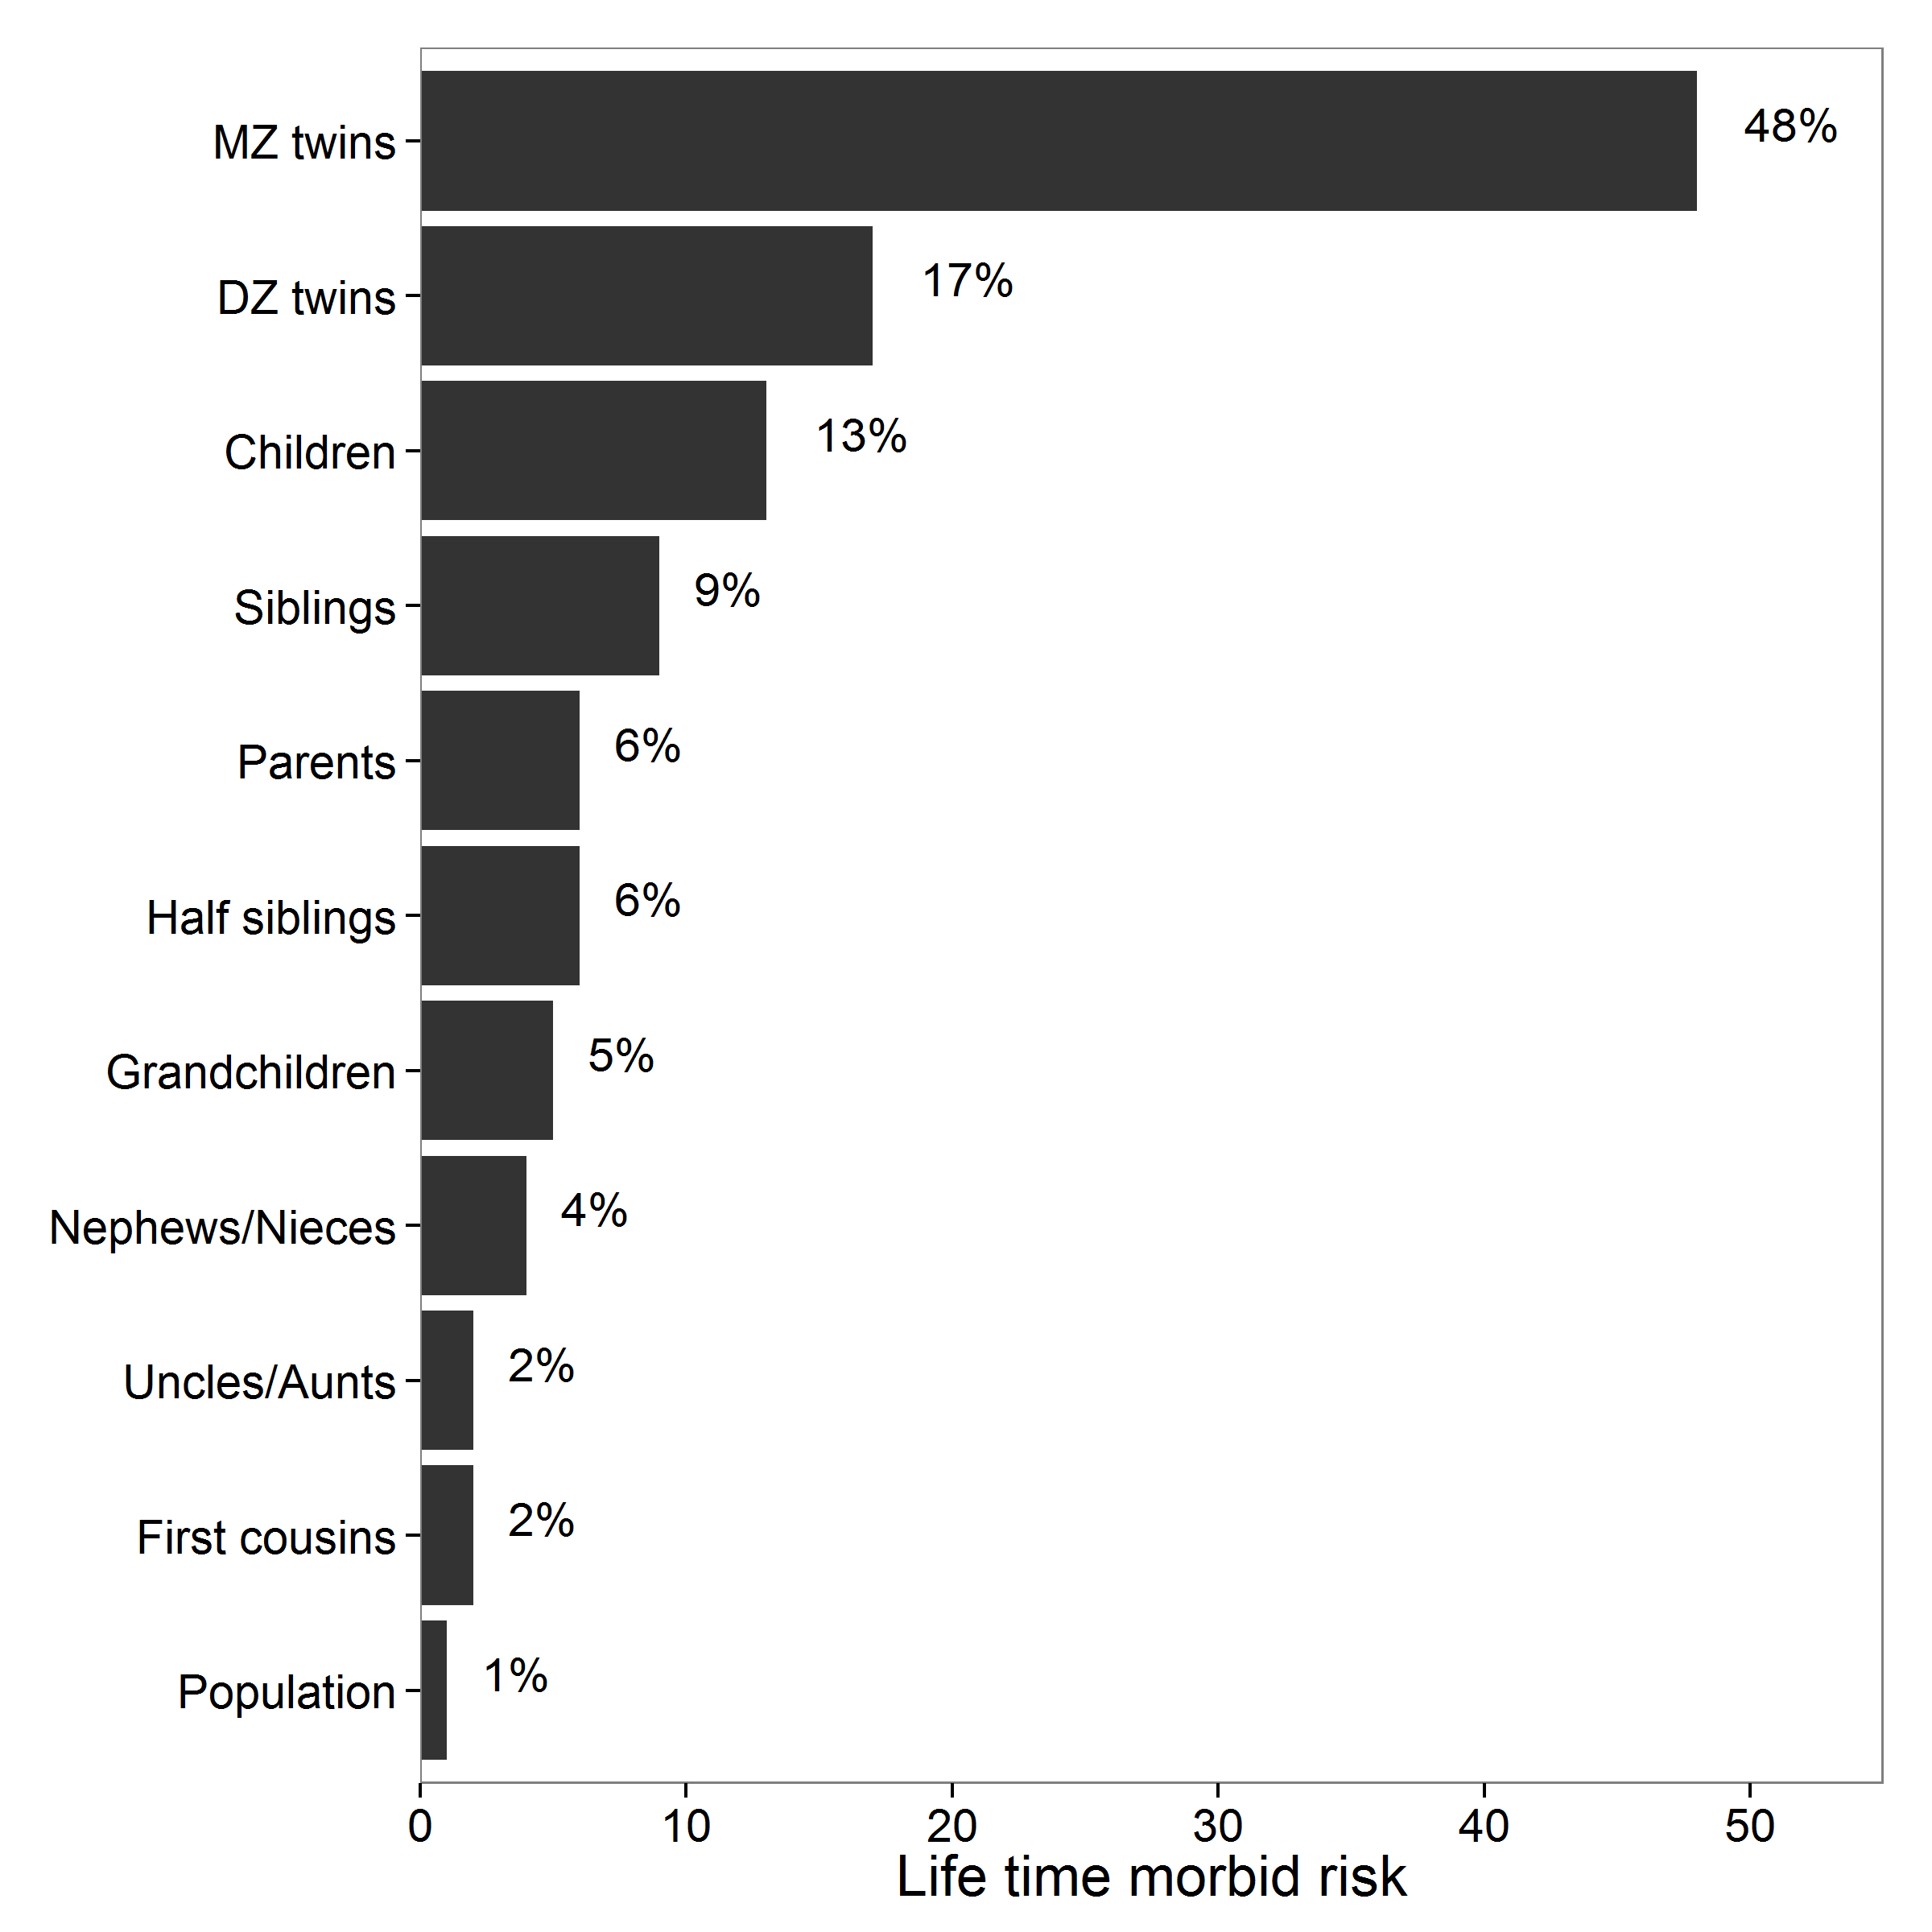
\includegraphics[width=0.6\textwidth]{figure/lifeTimeMorbidRisk.png}
		\caption[Lifetime morbid risks of \glng{scz} in various classes of relatives of a proband]{Lifetime morbid risks of \glng{scz} in various classes of relatives of a proband.
			It was noted that the morbid risk of \gls{mz} twins were only $48\%$, much lower than one would expect if \glng{scz} follows a Mendelian pattern.
			Reproduced with permission from journal \citep{Riley2006}. \label{fig:lifeMRscz}}
	\end{figure}
	
	In view of this, \citet{Gottesman1967} proposed that \glng{scz} follows a polygenic model, where the disease phenotype were determined by the additive effects from multiple genes.
	
	By comparing the observed lifetime morbid risk and the expected risk from different models, \citet{Risch1990} proposed that the cause variants of \glng{scz} are more likely to have a risk less than 2 with no loci with risk larger than 3, suggesting a relatively small effect size.
	Large sample size are therefore required to detect these susceptibility loci through linkage studies \citep{Risch1990}.
	
	This might explain the early inconsistent findings of linkage studies in \glng{scz} \citep{Harrison2005}.
	As genetic data from large, multi-generational pedigrees with both affected and unaffected individuals are required, subject recruitment of linkage studies are challenging. 
	With the small sample size and the relatively small effect expected in \glng{scz}, it is difficult for linkage studies to identify the susceptibility loci. 
	Other methods are therefore required to identify the susceptibility loci of \glng{scz}.
	
	
	\subsection{The Human Genome Project and HapMap Project}
	\glsreset{SNP}
	\glsreset{LD}
	In 1990, the Human genome project was initiated, aiming at constructing the first physical map of the human genome at per nucleotide resolution \citep{Lander2001}.
	The completion of the human genome project has opened up a new era of genetic research, allowing researchers to identify \glspl{SNP}, which is one of the major source of genetic variation in the human genome.
	
	Soon after the completion of the human genome project, the HapMap Project was initiated \citep{Consortium2005}, aiming to provide a genome-wide database of common human sequence variation such as \glspl{SNP} with \gls{maf} $\ge0.05$.
	
	More importantly, the HapMap Project provided a detailed \gls{LD} map of the human genome.
	\gls{LD} is important for genetic research as it is the non-random correlation of genotypes between 2 genetic loci. 
	\glspl{SNP} in high \gls{LD} are usually observed together in the human genome.
	When a large amount of \glspl{SNP} are in high \gls{LD} together, a \gls{LD} block is formed.
	By performing association testing on \glspl{SNP} representing majority of information within the \gls{LD} block (``tagging''), genome-wide association can be performed.
	This is the fundamental concept of \gls{GWAS}, which is now extensively used in genetic researches.
	
	\subsection{Genome Wide Association Study}
	In \gls{GWAS}, genome-wide genotyping array are commonly used to systematically detect common genetic variants such as \gls{SNP} and \gls{cnv} in genome-wide scale.
	For quantitative traits, the association between the trait and frequency of the variants are calculated using methods such as linear regression.
	On the other hand, for dichotomous traits such as \glng{scz}, the frequency of the variants are compared between the case and control samples using methods such as chi-square test or logistic regression.
	
	However, when a large number of \glspl{SNP} were tested, the frequency of type I error increases \citep{Peters2010}.
	Multiple testing correction is therefore vital in the analysis of \gls{GWAS}.
	
	The simplest method for the correction of \gls{GWAS} is to use the genome wide threshold (p-value $\le5\times10^{-8}$), where only \glspl{SNP} with p-value less then the genome wide threshold are considered to be significant in \gls{GWAS}.
	Another possible method to decide the significant threshold is to consider the ``effective number'' of tests \citep{Li2011}, which reduced the genome-wide threshold according to the \gls{LD} structure.
	
	Finally, when designing a \gls{GWAS}, the magnitude of effect, sample size, and required level of statistical significance (the false-positive, or type I, error rate) are all important factors determining the detection power of the \gls{GWAS} \citep{Purcell2003}.
	Similar to linkage studies, a larger sample size are required to identify susceptible loci with a smaller effect. 
	
	\subsubsection{The Success of Psychiatric Genomic Consortium} 
	Early \gls{GWAS} in \glng{scz} were largely disappointing, where no robust genetic markers associated with \glng{scz} were identified. 
	The main reason for the failure of the early \gls{GWAS} is the relatively small sample size.
	
	To overcome the problem of sample size, large consortium were formed such that genetic data from different research groups were combined and analyzed.
	Finally, in 2014, the \Glng{scz} Working group of the \gls{pgc} has conducted a multi-stage \glng{scz} \gls{GWAS} of up to 36,989 \glng{scz} samples and 113,075 controls \citep{Ripke2014}.
	A total of 128 linkage-disequilibrium-independent \glspl{SNP} were found to exceeded the genome-wide significance (p-value $\le 5\times10^{-8}$), corresponding to 108 independent genetic loci.
	75\% of these loci contain protein coding genes and a further 8\% of these loci were within 20 \gls{kb} of a gene. 
	It was found that genes involved in glutamatergic neurotransmission (e.g. \textit{GRM3}, \textit{GRIN2A} and \textit{GRIA1}), synaptic plasticity and genes encoding the voltage-gated calcium channel subunits (e.g. \textit{CACNA1C}, \textit{CACNB2} and \textit{CACNA1I}) were among the genes associated within these loci.
	Moreover, \glng{scz} association were significantly enriched at enhancers active in brain and enriched at enhancers active in tissues with important immune functions (\cref{fig:pgcEnrich}) \citep{Ripke2014}.
	
	\begin{figure}
		\centering
		\caption[Enrichment of enhancers of SNPs associated with Schizophrenia]{Enrichment of enhancers of SNPs associated with \glng{scz}. 
			It was observed that the largest enrichment were in cell lines related to the brain and in tissues with important immune functions. 
			Graphs reproduced with permission from the journal \citep{Ripke2014}.}
		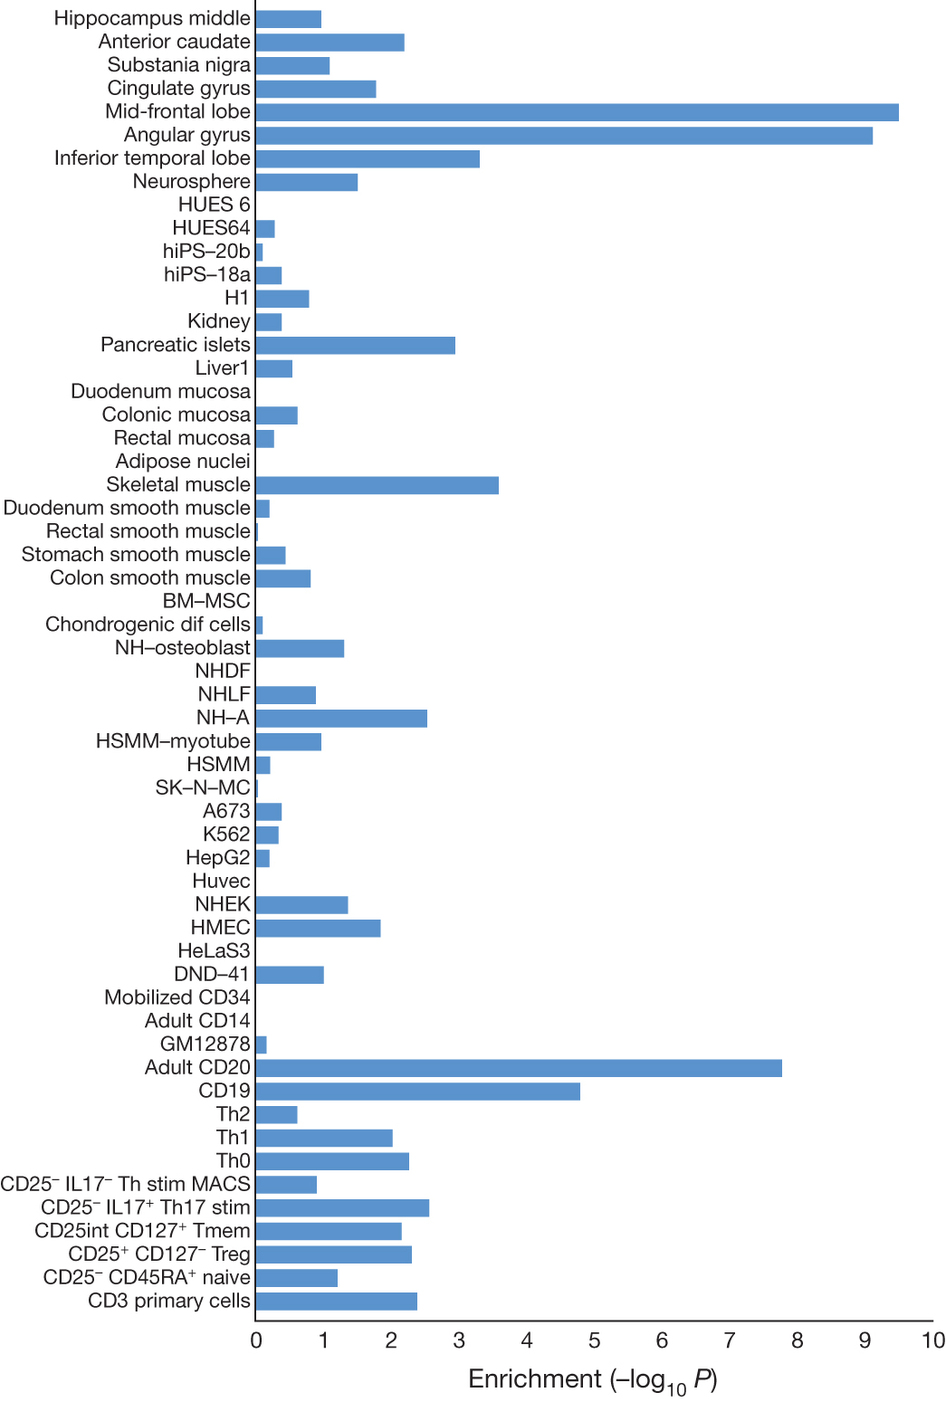
\includegraphics[height=\textwidth]{figure/pgc_enrichment_tissue.jpg}
		\label{fig:pgcEnrich}
	\end{figure}
	
	The enrichment of immune related enhancers remains significant even after the removal of \gls{mhc} region from the analysis, suggesting that the significance association of the immune system with \glng{scz} is not driven only by the \gls{mhc} region.
	Considering the role of immune system in neural development \citep{Zhao1998,Deverman2009}, perturbation in the immune system is likely to disrupts the brain development.
	Therefore, the immune system might have an important role in the etiology of \glng{scz}.
	%Indeed, studies on \gls{mia} has demonstrated that cytokine imbalance might predispose individual to \glng{scz} \citep{Meyer2009}. 
%	
%	Moreover, \textit{DRD2}, the target of all effective anti-psychotic drug were also found to be associated with \glng{scz}.
%	This result converges with existing knowledge of \textit{DRD2} being involved in the pathology of \glng{scz}, supported by multiple lines of research \citep{Talkowski2007}.
	
	
	Despite the success of \gls{pgc} \glng{scz} \gls{GWAS}, it is uncertain whether if all common variants associated with \glng{scz} has been captured. 
	With the unknown number of causal loci with moderate-to-small effect size, many \glspl{SNP} associated with \glng{scz} may be left undetected with the current sample size. 
	However, it is also possible that the \gls{pgc} \glng{scz} \gls{GWAS} has already captured all or near most of the \glspl{SNP} associated with the disease. 
	Therefore, estimating the contribution of these common \glspl{SNP} to \glng{scz} has important implications for future research strategy.
	
	\subsection{Contribution of Common SNPs}
	\gls{GWAS} usually imposes a stringent genome wide significant threshold to avoid false positive findings. 
	However, if individual \glspl{SNP} have a small effect on the trait, the real association might be filtered.
	Therefore, to estimate the true contribution of common \glspl{SNP} to a disease (\gls{SNP}-heritability), it is important to consider all the \glspl{SNP} in the estimation.
	
	\subsubsection{Genome-wide Complex Trait Analysis}
	Currently, the most popular algorithm for the estimation of \gls{SNP}-heritability is \gls{gcta}, which utilize information from the \gls{grm} \citep{Yang2011}.
	The \gls{grm} represents the ``genetic distance'' between all individuals within the \gls{GWAS}.
	Genetic relationship between individual $j$ and $k$ is estimated as 
	\begin{equation}
	A_{jk} = \frac{1}{N}\sum^N_{i=1}\frac{(x_{ij}-2p_i)(x_{ik}-2p_i)}{2p_i(1-p_i)}
	\end{equation}
	where $x_{ij}$ is the number of copies of the reference allele for the $i^{th}$ \gls{SNP} of the $j^{th}$ individual and $p_i$ is the frequency of the reference allele.
	Because genotypes are usually code as 0, 1 or 2 (homozygous reference, heterozygous and homozygous alternative respectively), they follow the binomial distribution.
	Therefore, the expected mean and variance of genotype $i$ is $2p_i$ and $2p_i(1-p_i)$ respectively, and the \gls{grm} can be represented as $A_{jk} = \frac{1}{N}\sum^N_{i=1}z_{ij}z_{ik}$, where $z_{ij}$ is the standardized genotype for the $i^{th}$ \gls{SNP} of the $j^{th}$ individual.
	
	Using the information from the \gls{grm}, \citet{Yang2011} fitted the effects of all the \glspl{SNP} as random effects by a \gls{mlm}
	\begin{align}
	\boldsymbol{y} &= \boldsymbol{X\beta}+\boldsymbol{g}+\epsilon\\
	\mathrm{Var}(\boldsymbol{y}) &= \boldsymbol{A}\sigma_g^2+\boldsymbol{I}\sigma_\epsilon^2
	\end{align}
	where $\boldsymbol{y}$ is an $n\times 1$ vector of phenotypes with $n$ samples, $\boldsymbol{\beta}$ is a vector of fixed effects such as sex and age, $\boldsymbol{g}$ is an $n\times 1$ vector of the total genetic effects of the individuals, $\sigma_g^2$ is the variance explained by all the \glspl{SNP} and finally, $\sigma_\epsilon^2$ is the variance explained by residual effects.

	The main concept of \gls{gcta} is that instead of testing the associations for individual \glspl{SNP}, effects of \emph{all} \glspl{SNP} are fit as random effects in a \gls{mlm}, such that a single parameter can be estimated, i.e. the variance explained by all \glspl{SNP} or \gls{SNP}-heritability.
	Given the information of the \gls{grm}, \citet{Yang2011} implemented the \gls{reml} using the average information algorithm to estimate the $\sigma_g^2$ and $\sigma_\epsilon^2$, where the \gls{reml} is a form of maximum likelihood estimation that allows unbiased estimates of variance and covariance parameters.
	The \gls{SNP}-heritability of the trait is then defined as $\frac{\sigma_g^2}{\sigma_g^2+\sigma_e^2}$.

	\citet{Yang2010a} were able to estimate the variance in height explained by \glspl{SNP} from the height \gls{GWAS} to be around 45\%, much larger than previously reported 5\%.
	Although the estimates was still less than 80\%, which is the expected heritability of height, \citet{Yang2010a} was able to demonstrated that one possible source of ``missing heritability'' might were due to incomplete \gls{LD}.
	By considering incomplete \gls{LD}, \citet{Yang2010a} estimated that the proportion of variance explained by causal variants can be as high as 0.84 with \gls{se} of 0.16, which is closer to the heritability of height.
	
	An limitation of \gls{gcta} is that genotype data are required to calculate the \gls{grm}.
	For studies which only summary statistics are available, for example, the meta-analysis of \glng{scz}, \gls{gcta} analysis cannot be performed.
	
	\subsubsection{\glng{ldsc}}
	In large scale \gls{GWAS} studies, a general inflation of summary statistics can sometimes be observed.
	The inflation was usually considered to be contributed by the presence of confounding factors such as population stratification, under the assumption that most of the \glspl{SNP} were not associated with the disease.
	Therefore, \gls{gc} inflation factor were usually used to control for the inflation in \gls{GWAS} results \citep{Zheng2006}.
	
	However, the assumption of a small number of causal \glspl{SNP} might not be true, especially for complex disease such as \glng{scz}.
	Through careful simulation, \citet{Yang2011b} demonstrated that in the absence of population stratification and other form of technical artifacts, the presence of polygenic inheritance can inflate the summary statistic.
	It was observed that the magnitude of inflation was determined by the \emph{heritability}, the \gls{LD} structure, sample size and the number of causal \glspl{SNP} of the trait.
%	
%	The observation of \citet{Yang2011b} provided important foundation for the estimation of \gls{SNP} heritability based on summary statistics.
%	By delineating the contribution from confounding factors and common 
%	 where a possible method will be to elucidate the heritability based on the magnitude of inflation of the summary statistics. 
%	However, when confounding factors such as population stratification and cryptic relatedness are presented, they can also inflate the summary statistics.
%	Therefore, in order to estimate the \gls{SNP}-heritability, one must delineate the confounding factors from the polygenicity of the trait.
	
	Based on the work of \citet{Yang2011b}, \citet{Bulik-Sullivan2015} hypothesized that the probability of a \gls{SNP} to be a neighbor of the causal variant is higher if the \gls{SNP} is in \gls{LD} with a larger number of \glspl{SNP}.
	However, this probability should be independent of the confounding factors such as population stratification and cryptic relatedness.
	%TODO here
	Therefore, \citet{Bulik-Sullivan2015} developed the \gls{LD} score.
	The \gls{LD} score of a \gls{SNP} $j$ is defined as the sum of $r^2$ of $k$ neighboring \glspl{SNP} within a 1 \gls{cm} window:
	\begin{equation}
	l_j = \sum_kr^2_{jk}
	\label{eq:ldScore}
	\end{equation}
	
	The expected $\chi^2$ of association of \gls{SNP}$_j$ with the trait can then be defined as a function of the \gls{LD} score ($l_j$), the number of samples ($N$), the number of \glspl{SNP} in the analysis ($M$) and most importantly, the \gls{SNP} heritability ($h^2$):
	\begin{equation}
	\mathrm{E}[\chi^2_j | l_j] = \frac{Nh^2}{M}l_j+1
	\label{eq:fixedLDSC}
	\end{equation}
	
	When confounding factors present in the study (e.g. population stratification), \cref{eq:fixedLDSC} can instead be defined as
	\begin{equation}
	\mathrm{E}[\chi^2_j | l_j] = \frac{Nh^2}{M}l_j+Na+1
	\label{eq:fullLDSC}
	\end{equation}
	where $a$ is the contribution of confounding bias.
	
	By considering \cref{eq:fullLDSC} as a regression model, \citet{Bulik-Sullivan2015} observed that the contribution of common variants (the \gls{SNP} heritability $h^2$) will be the slope of the regression, whereas the intercept minus one will represent the mean contribution of the confounding bias, such as population stratification. 
	The \gls{ldsc} was then implemented using \cref{eq:fullLDSC} to delineate the contribution from confounding factors and common genetic variants \citet{Bulik-Sullivan2015}.
	
	To test whether \gls{ldsc} can truly delineate the contribution from confounding factors and common genetic variants, \citet{Bulik-Sullivan2015} performed a series of simulation.
	When the simulated traits are polygenic and no confounding factors are presented, the average \gls{ldsc} intercept was close to one and the estimates were unbiased in all situation.
	Only when the number of causal variants was small will the standard error of the estimates become very large.
	On the other hand, when the \gls{GWAS} was simulated with only the confounding factors such as population stratification, the intercept estimated was approximately equal to the \gls{gc} inflation factor, with only a small positive bias in the regression slope.
	
	Furthermore, when polygenic traits were simulated with confounding factors, the intercept of \gls{ldsc} was approximately equal to the mean $\chi^2$ statistic among the null \glspl{SNP}, providing strong evidence that \gls{ldsc} can partition the inflation in test statistic, even in the presence of both bias and polygenicity.
	
	\citet{Bulik-Sullivan2015} then estimated the \gls{SNP} heritability of \glng{scz}, using the summary statistics from the \gls{pgc} \glng{scz} \gls{GWAS} \citep{Ripke2014}.
	It is estimated that the \gls{SNP} heritability of \glng{scz} is 0.555 with \gls{se} of 0.008 after adjusting for ascertainment bias.
	The estimated \gls{SNP} heritability was lower than the heritability estimated from population based study (64\% \citep{Lichtenstein2009}) and twin studies (81\% \citep{Sullivan2003}).
	Therefore, it is possible for variants other than common \glspl{SNP} to account for the heritability of \glng{scz}.
	
	\subsubsection{Partitioning of Heritability}
	Another implication of \gls{ldsc} is that it allows the partitioning of heritability, which helps to identify pathways that are associated with a trait.
	
	Traditionally, functional enrichment analysis in \gls{GWAS} only consider \glspl{SNP} that passed the genome wide significance threshold. 
	However, for complex traits such as \glng{scz}, it is possible that some of the \glspl{SNP} with small effect size do not reach genome wide significance threshold at the current sample size.
	For example, in 2013, only 13 risk loci were detected using 13,833 \glng{scz} samples and 18,310 controls \citep{Ripke2013}. 
	When the sample size increased to 34,241 \glng{scz} samples and 45,604 controls in 2014, 108 risk loci were identified \citep{Ripke2014}. 
	Thus, by only selecting \glspl{SNP} passing the genome wide significant thresholds, some of the risk loci might be ignored from the functional enrichment analysis.
	
	To estimate whether a functional category is associated with the trait, \gls{ldsc} utilize the summary statistic of all the \glspl{SNP} included in the \gls{GWAS}.
	The partitioning of the heritability is then calculated as 
	\begin{equation}
	\mathrm{E}[\chi^2_j] = N\sum_C\tau_Cl(j,C)+Na+1
	\label{eq:partitionH}
	\end{equation}
	
	The main difference between \cref{eq:partitionH} and \cref{eq:fullLDSC} is that $\frac{h^2}{M}l_j$ is substituted by $\sum_C\tau_Cl(j,C)$ where $l(j,C)$ is the \gls{LD} Score of \gls{SNP} $j$ with respect to category $C$ and $\tau C$ is the per-\gls{SNP} heritability in category $C$.
	
	Using data from \citet{Ripke2014}, and functional categories derived from the ENCODE annotation \citep{ENCODEProjectConsortium2012}, the NIH Roadmap Epigenomics Mapping Consortium annotation \citep{Bernstein2010} and other studies, \citet{Finucane2015} attempted to identify functional categories that were most enriched in \glng{scz}.
	\citet{Finucane2015} found that brain cell types and immune related cell types were most enriched in \glng{scz}.
	Among the functional categories, the most enriched category in \glng{scz} was the H3K4me3 mark in the fetal brain (\cref{tab:cellTypeScz}). 
	As H3K4me3 is mostly linked to active promoters, it is possible that genes activated in fetal brain (e.g. genes related to brain development) are associated with \glng{scz}, supporting the idea of \glng{scz} as a neuro-developmental disorder. 
	
	\begin{singlespace}
		\begin{longtable}{p{6cm}rrr}
			%\begin{tabular}{rrrr}
			\toprule
			Cell type & cell-type group & Mark  & P-value \\
			\midrule
			Fetal brain** & CNS   & H3K4me3 & $3.09\times 10^{-19}$ \\
			Mid frontal lobe** & CNS   & H3K4me3 & $3.63\times 10^{-15}$ \\
			Germinal matrix** & CNS   & H3K4me3 & $2.09\times 10^{-13}$ \\
			Mid frontal lobe** & CNS   & H3K9ac & $5.37\times 10^{-12}$ \\
			Angular gyrus** & CNS   & H3K4me3 & $1.29\times 10^{-11}$ \\
			Inferior temporal lobe** & CNS   & H3K4me3 & $1.70\times 10^{-11}$ \\
			Cingulate gyrus** & CNS   & H3K9ac & $5.37\times 10^{-11}$ \\
			Fetal brain** & CNS   & H3K9ac & $5.75\times 10^{-11}$ \\
			Anterior caudate** & CNS   & H3K4me3 & $2.19\times 10^{-10}$ \\
			Cingulate gyrus** & CNS   & H3K4me3 & $4.57\times 10^{-10}$ \\
			Pancreatic islets** & Adrenal/Pancreas & H3K4me3 & $2.24\times 10^{-09}$ \\
			Anterior caudate** & CNS   & H3K9ac & $3.16\times 10^{-9}$ \\
			Angular gyrus** & CNS   & H3K9ac & $4.68\times 10^{-9}$ \\
			Mid frontal lobe** & CNS   & H3K27ac & $7.94\times 10^{-9}$ \\
			Anterior caudate** & CNS   & H3K4me1 & $1.20\times 10^{-8}$ \\
			Inferior temporal lobe** & CNS   & H3K4me1 & $3.72\times 10^{-8}$ \\
			Psoas muscle** & Skeletal Muscle & H3K4me3 & $4.17\times 10^{-8}$ \\
			Fetal brain** & CNS   & H3K4me1 & $6.17\times 10^{-8}$ \\
			Inferior temporal lobe** & CNS   & H3K9ac & $9.33\times 10^{-8}$ \\
			Hippocampus middle** & CNS   & H3K9ac & $9.33\times 10^{-7}$ \\
			Pancreatic islets** & Adrenal/Pancreas & H3K9ac & $1.62\times 10^{-6}$ \\
			Penis foreskin melanocyte primary** & Other & H3K4me3 & $2.09\times 10^{-6}$ \\
			Angular gyrus** & CNS   & H3K27ac & $2.34\times 10^{-6}$ \\
			Cingulate gyrus** & CNS   & H3K4me1 & $2.82\times 10^{-6}$ \\
			Hippocampus middle** & CNS   & H3K4me3 & $2.82\times 10^{-6}$ \\
			CD34 primary** & Immune & H3K4me3 & $4.68\times 10^{-6}$ \\
			Sigmoid colon** & GI    & H3K4me3 & $5.01\times 10^{-6}$ \\
			Fetal adrenal** & Adrenal/Pancreas & H3K4me3 & $6.31\times 10^{-6}$ \\
			Inferior temporal lobe** & CNS   & H3K27ac & $8.32\times 10^{-6}$ \\
			Peripheralblood mononuclear primary** & Immune & H3K4me3 & $9.33\times 10^{-6}$ \\
			Gastric** & GI    & H3K4me3 & $1.17\times 10^{-5}$ \\
			Substantia nigra* & CNS   & H3K4me3 & $1.95\times 10^{-5}$ \\
			Fetal brain* & CNS   & H3K4me3 & $2.63\times 10^{-5}$ \\
			Hippocampus middle* & CNS   & H3K4me1 & $3.31\times 10^{-5}$ \\
			Ovary* & Other & H3K4me3 & $6.46\times 10^{-5}$ \\
			CD19 primary (UW)* & Immune & H3K4me3 & $7.08\times 10^{-5}$ \\
			Small intestine* & GI    & H3K4me3 & $8.51\times 10^{-5}$ \\
			Lung* & Cardiovascular & H3K4me3 & $1.17\times 10^{-4}$ \\
			Fetal stomach* & GI    & H3K4me3 & $1.29\times 10^{-4}$ \\
			Fetal leg muscle* & Skeletal Muscle & H3K4me3 & $1.51\times 10^{-4}$ \\
			Spleen* & Immune & H3K4me3 & $1.70\times 10^{-4}$ \\
			Breast fibroblast primary* & Connective/Bone & H3K4me3 & $2.04\times 10^{-4}$ \\
			Right ventricle* & Cardiovascular & H3K4me3 & $2.14\times 10^{-4}$ \\
			CD4+ CD25- Th primary* & Immune & H3K4me3 & $2.19\times 10^{-4}$ \\
			CD4+ CD25- IL17- PMA Ionomycin stim MACS Th sprimary* & Immune & H3K4me1 & $2.19\times 10^{-4}$ \\
			CD8 naive primary (UCSF-UBC)* & Immune & H3K4me3 & $2.24\times 10^{-4}$ \\
			Pancreas* & Adrenal/Pancreas & H3K4me3 & $2.34\times 10^{-4}$ \\
			CD4+ CD25- Th primary* & Immune & H3K4me1 & $2.75\times 10^{-4}$ \\
			CD4+ CD25- CD45RA+ naive primary* & Immune & H3K4me1 & $2.75\times 10^{-4}$\\
			Colonic mucosa* & GI    & H3K4me3 & $3.24\times 10^{-4}$ \\
			Right atrium* & Cardiovascular & H3K4me3 & $3.31\times 10^{-4}$ \\
			Fetal trunk muscle* & Skeletal Muscle & H3K4me3 & $3.39\times 10^{-4}$ \\
			CD4+ CD25int CD127+ Tmem primary* & Immune & H3K4me3 & $3.47\times 10^{-4}$ \\
			Substantia nigra* & CNS   & H3K9ac & $3.63\times 10^{-4}$ \\
			Placenta amnion* & Other & H3K4me3 & $4.17\times 10^{-4}$ \\
			Breast myoepithelial* & Other & H3K9ac & $5.50\times 10^{-4}$ \\
			CD8 naive primary (BI)* & Immune & H3K4me1 & $5.75\times 10^{-4}$ \\
			Substantia nigra* & CNS   & H3K4me1 & $6.61\times 10^{-4}$ \\
			Cingulate gyrus* & CNS   & H3K27ac & $7.94\times 10^{-4}$ \\
			CD4+ CD25- CD45RA+ naive primary* & Immune & H3K4me3 & $8.71\times 10^{-4}$ \\
			\bottomrule
				%\end{tabular}%
			\caption[Enrichment of Top Cell Type of Schizophrenia]{Enrichment of Top Cell type of Schizophrenia.
				* = significant at False Discovery Rate $<$ 0.05.
				** = significant at p $<$ 0.05 after correcting for multiple hypothesis. 
				Reproduce with permission from Journal.\citep{Finucane2015}}
			\label{tab:cellTypeScz}%
		\end{longtable}%
	\end{singlespace}
		
	\subsection{Rare Variants in Schizophrenia}
	\glsreset{cnv}
	The heritability estimates from \citet{Bulik-Sullivan2015} using the \gls{pgc} \gls{GWAS} data suggested that common \glspl{SNP} have relatively less contribution ot the genetic predisposition of individuals to \glng{scz}.
	Therefore, it is possible that rare variants might also contributes to the heritability of \glng{scz}.
	
	\subsubsection{Copy Number Variation}
	A possible source of rare variants is \glspl{cnv}.
	\gls{cnv} are classified as segment of DNA that is 1 \gls{kb} or larger, and is present at a different copy number when compared to the reference genome, usually in the form of insertion, deletion or duplication \citep{Feuk2006}.
	Due to the length of these variants, the \gls{cnv} might contain the entire genes and their regulatory regions, which might in turn contribute to significant phenotypic differences \citep{Feuk2006}.
	
	Recently, \citet{Szatkiewicz2014} conducted a \gls{GWAS} for \gls{cnv} association with \glng{scz} using the Swedish national sample (4,719 \glng{scz} samples and 5,917 controls).
	\citet{Szatkiewicz2014} were able to identify association between \glng{scz} and \glspl{cnv} such as 16p11.2 duplications, 22q11.2 deletions, 3q29 deletions and 17q12 duplications.
	Through the gene set association analysis, calcium channel signaling and binding partners of the fragile X mental retardation protein were found to be enriched by \gls{cnv} observed in schizophrenic samples \citep{Szatkiewicz2014}.
	Interestingly, in the \gls{pgc} \glng{scz} \gls{GWAS}, association was observed genes encoding the voltage-gated calcium channel subunits.
	The results indicated that both common variants and \gls{cnv} may be affecting the same set of pathways or gene sets in the etiology of \glng{scz}.
	
	Similarly, \citet{Walsh2008} also found that genes disrupted by structure variants in schizophrenic samples were significantly overrepresented in pathways important for brain development, including neuregulin signaling, extracellular signal-regulated kinase/\gls{mapk} signaling, synaptic long-term potentiation, axonal guidance signaling, integrin signaling, and glutamate receptor signaling.
	
	In general, \glspl{cnv} associated with \glng{scz} were rare ($\le12$ in 4,719 samples \citep{Szatkiewicz2014}) and have a relative large effect (e.g. odd ratio $>2$ \citep{Szatkiewicz2014,Walsh2008}).
	
	\subsubsection{Rare Single Nucleotide Mutation}
	Unlike \gls{cnv}, which affects a large region, rare \glspl{SNP} cannot be captured using current genotyping chips.
	Therefore, large scale association of rare \glspl{SNP} was unavailable until the development of the \gls{ngs} technology.
	Recent progress in \gls{ngs} has enabled the sequencing of the whole genome or exome, providing a per-base resolution, therefore allow for the identification of rare genetic variants without requiring ``tagging''.
	
	Using exome sequencing, \citet{Purcell2014} sequenced the exome of 2,536 \glng{scz} cases and 2,543 normal controls. 
	\citet{Purcell2014} identified a common missense allele on \textit{CCHCR1} in the \gls{mhc} to be associated with \glng{scz}.
	Although none of the genes showed a significant burden of rare mutation in \glng{scz} cases, a significant increased burden of rare nonsense and disruptive variants was observed in gene sets such as voltage-gated calcium ion channel, genes affected by \textit{de novo} mutations in \glng{scz} \citep{Fromer2014} and the postsynaptic density, all of which have been reported to be associated with \glng{scz} in previous genetic studies \citep{Ripke2014}.

	The overlaps between the rare variant studies and the common variant studies suggest that both rare and common variants are likely to be acting upon the same pathway and are complementary to each other.
	
	\section{Environmental Risk Factors of Schizophrenia}
	Apart from genetic variants, another possible source of the ``missing'' heritability can come from interaction between the genetic and environmental risk factors.
	Although previous studies \citep{Gottesman01071967} suggested that the non-additive genetic factors were unlikely to contribute to \glng{scz}, the possibility of the involvement of gene-environmental interaction ($G\times E$) were not ruled out.
	Indeed, in the adoption study conducted by \citet{Tienari2004}, it was found that individuals with higher genetic risk were significantly more sensitive to ``adverse'' vs ``healthy'' rearing patterns in adoptive families than are adoptees at low genetic risk \citep{Tienari2004}.
	Moreover, using the national registers in Finland, \citet{Clarke2009} found that the effect of prenatal infection was five times greater in those who had a family history of psychosis when compared to those who did not. 
	Together, these findings support a mechanism of gene-environment interaction in the causation of \glng{scz}.
	
	Many environmental factors have been associated with \glng{scz}, including prenatal infection \citep{Brown2010}, winter birth \citep{OCallaghan1991}, tobacco consumption \citep{Kelly1999} and socio economic status \citep{McGrath2008a}.
	These environmental factors are therefore potential targets for the study of $G\times E$ interaction.
	However, by and large, the prenatal infection is the largest environmental risk factor of \glng{scz}.
	Furthermore, existing evidence indicated that there are an interaction between prenatal infection and genetic variations \citep{Clarke2009}.
	Investigation on how prenatal infection trigger \glng{scz} and how it interacts with genetic variations in the development of \glng{scz} are therefore important.	
	
	\subsection{Prenatal Infection}
	\begin{figure}
		\centering
		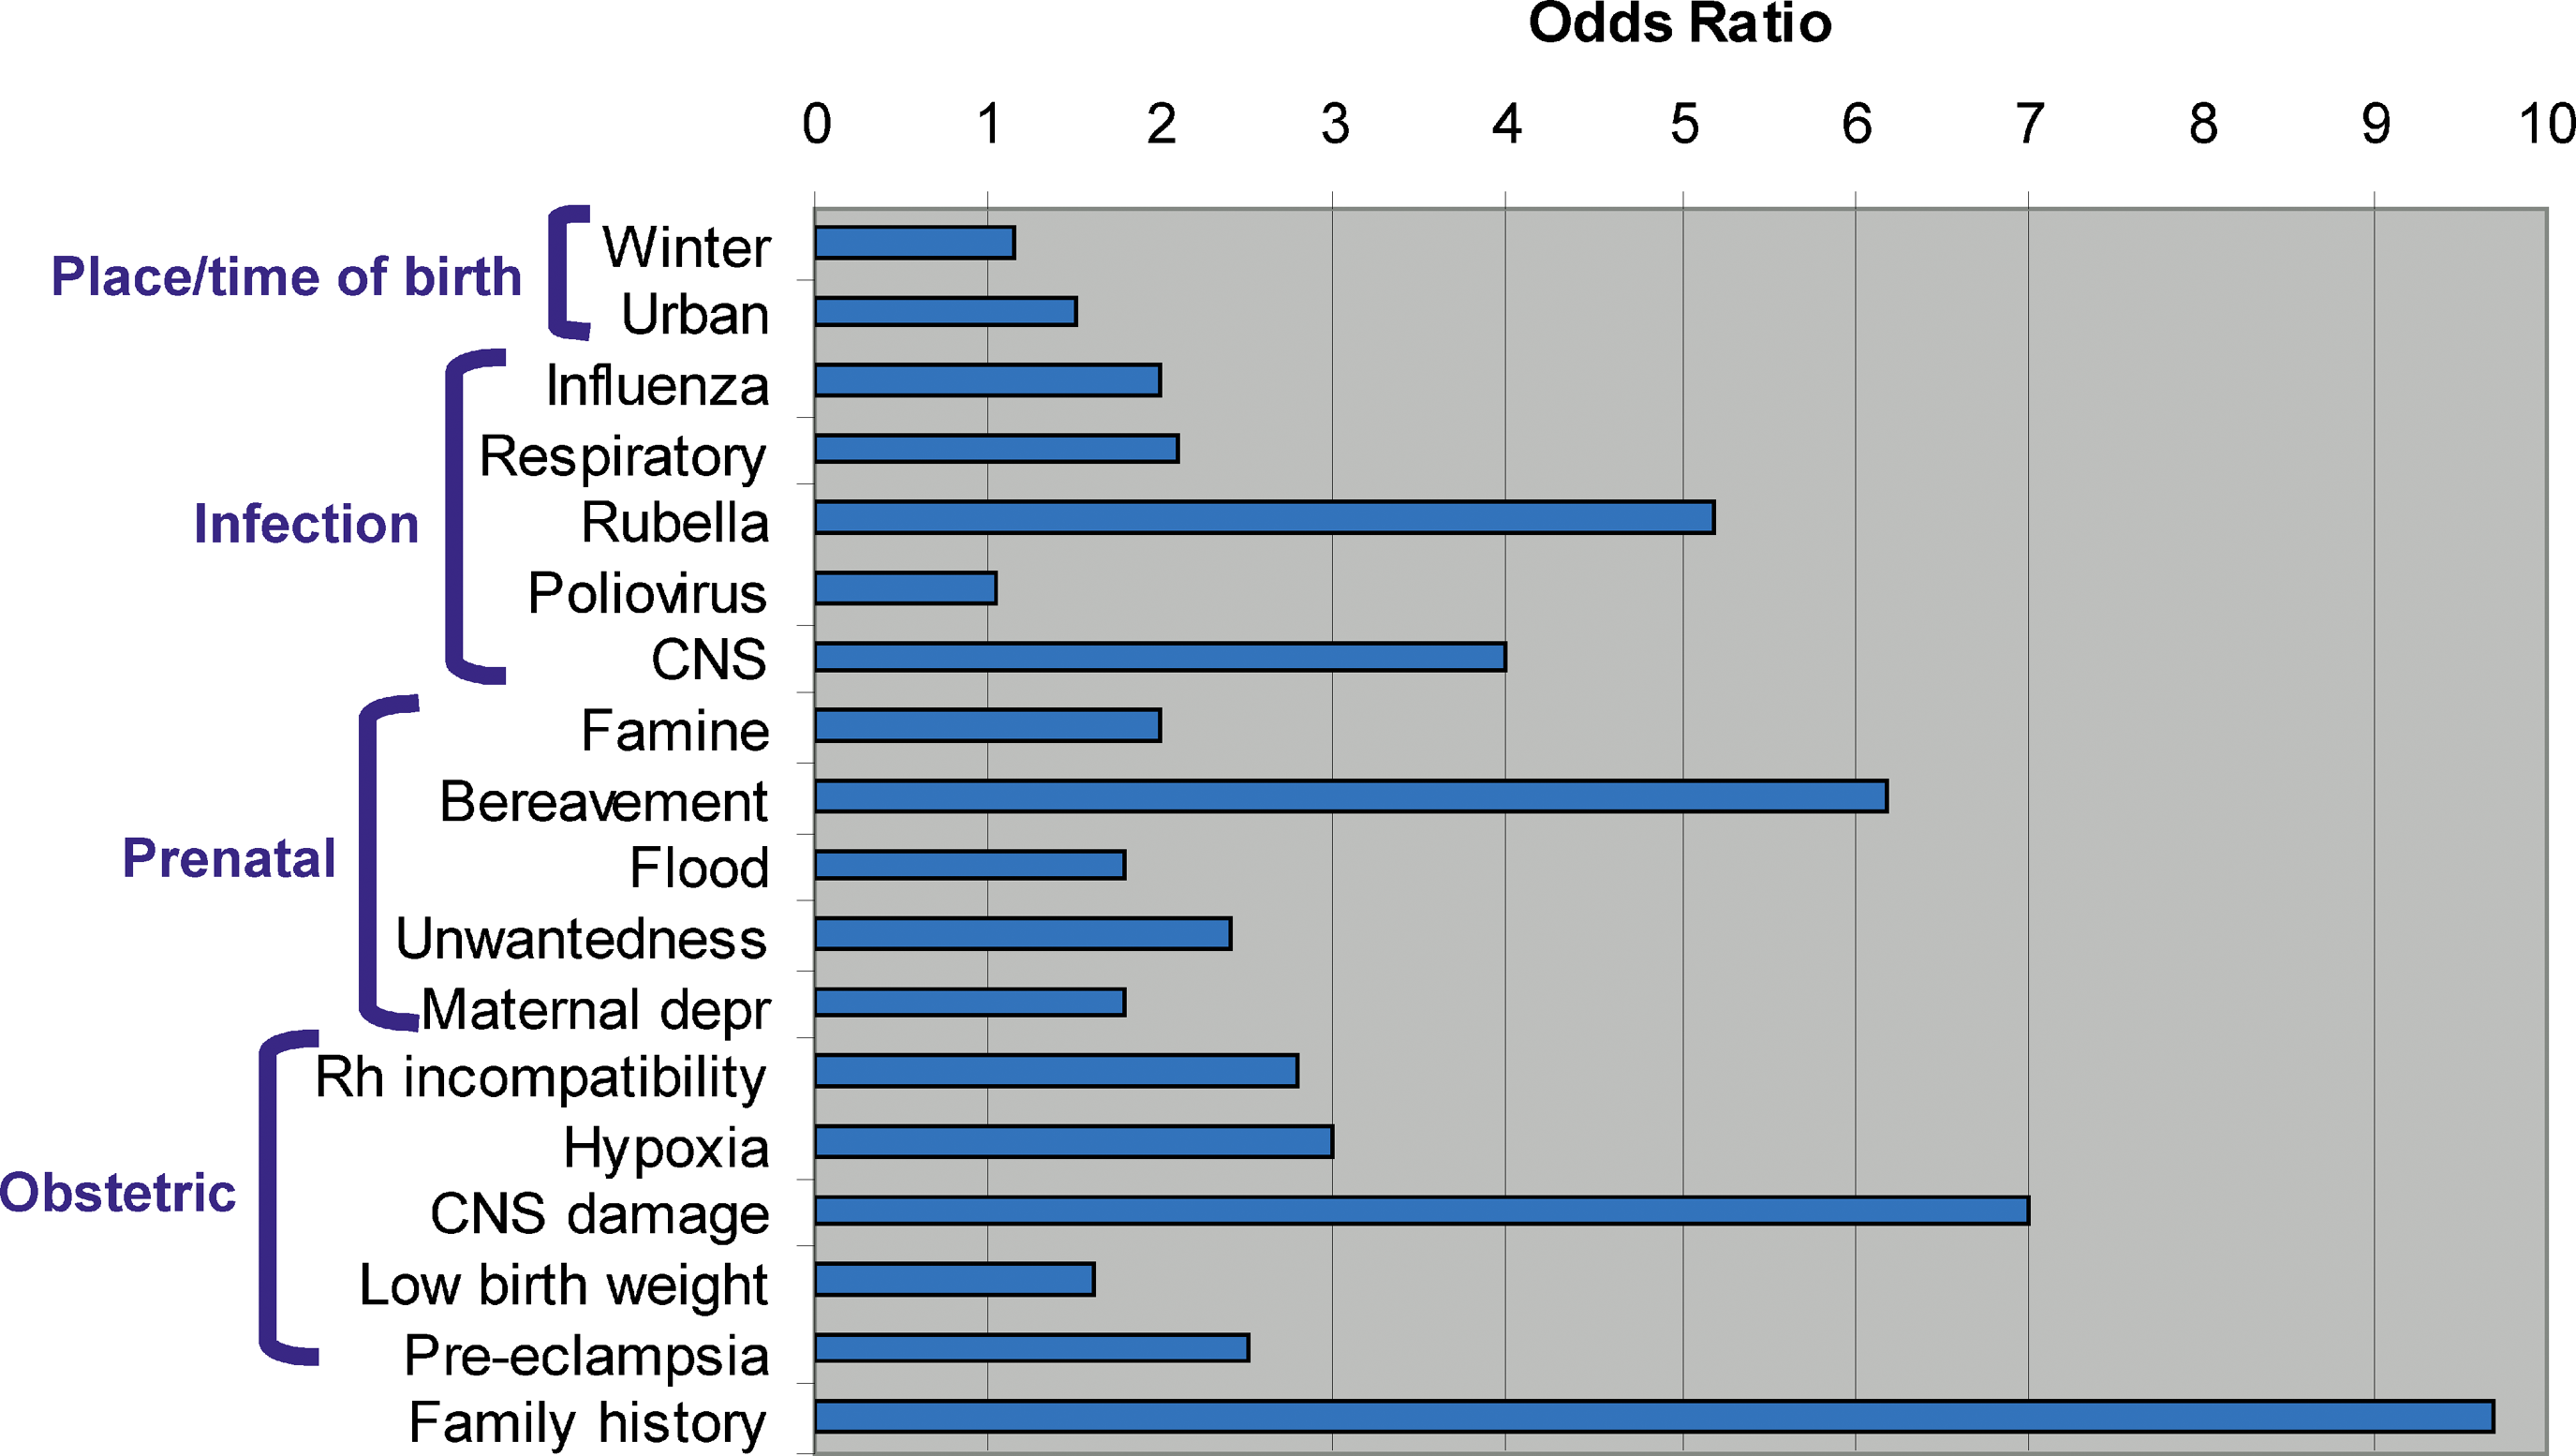
\includegraphics[width=\textwidth]{figure/risk_factors_of_schizophrenia.png}
		\caption[Risk factors of \glng{scz}]{Risk factors of \glng{scz}.
			It was observed that family history of \glng{scz} was the largest risk factors.
			Risk of \glng{scz} can be more than 9 times higher than the general population for individual with a family history of \glng{scz}}
		\label{fig:riskfactors}
	\end{figure}
	Prenatal infection is the single largest non-genetic risk factor of \glng{scz} (\cref{fig:riskfactors}) \citep{Sullivan2005}.
	Initial clues of an involvement of prenatal infection in the etiology of \glng{scz} comes from the observations that births during the winter and spring months; and births in urban areas were related to an increased risk of the disorder \citep{Brown2010}.
	It was also observed that there was an increased risk of \glng{scz} in individuals who were fetuses during the 1957 influenza epidemic \citep{Mednick1958}.
	As the chance of getting infectious diseases varies by season, and infectious diseases spread faster in urban regions due to higher population density, these evidences suggested that prenatal infection might be associated with \glng{scz}.
	
	Early studies of prenatal infection in \glng{scz} mainly relies on ecological data such as influenza epidemics in the population to define the exposure status \citep{Brown2010}.
	The problem of these studies was that the exposure status was based solely on whether an individual was in gestation at the time of the epidemic without any confirmation of maternal infection during pregnancy.
	Therefore, the exposure status might be inaccurate and unreliable, leading to difficulties in replication of the findings from these epidemiological studies \citep{Brown2010}.  
	Subsequently, birth cohorts, where infection was documented using different biomarkers during pregnancies, were conducted in order to obtain a better labeling of the exposure status \citep{Brown2010}.
	It was found that the risk of \glng{scz} increases as long as an individual's mother was infected by any form of infectious agents such as influenza, HSV-2 and \textit{T.gondii} during gestation \citep{Brown2010}.
	As various infectious agents increase the risk of \glng{scz}, it leads to the hypothesis that \gls{mia} \citep{Brown2010} rather than a particular infectious agent, is the source of risk factor. 
	It was suggested that the maternal immune response to the infection might have disrupted the brain development in the fetus, thus leading to an elevated risk of \glng{scz} \citep{Garbett2012a}.
	
	A great challenge in the study of \gls{mia} is that it is not possible to carry out controlled experiment on human samples due to ethical concerns.
	Thus, a popular alternative is to employ rodent models.
	However, unlike physiological traits, psychiatric disorder such as \glng{scz} are characterized by symptoms related to higher level functioning such as hallucinations, delusion, disorganized speech etc \citep{AmericanPsychiatricAssociation2013}, which are not readily detectable in rodents.
	This raises challenge in diagnosing whether the rodent is schizophrenic or not.
	Therefore, the phenotypes of rodent samples are usually defined by the expression ``schizophrenia-like'' behaviours such as impaired prepulse inhibition, impaired working memory and reduced social interaction \citep{Meyer2007a}.
	
	However, the behavioral abnormality is not unique to \glng{scz}, but can also be observed in autistic samples.
	Moreover, risk of autism is also increased by \gls{mia} \citep{Brown2012}.
	As a result, studies using these rodent models were non-specific to \glng{scz} or autism. 
	However, the discussion of the etiology of autism and the similarity and difference between autism and \glng{scz} is beyond the scope of the current thesis.
	Therefore, we will limit our discussion to \glng{scz}.
	
	A common rodent model in the study of effect of \gls{mia} is to use the viral analogue \gls{polyic} to induce the maternal immune response during pregnancy.
	It was found that offspring exposed to \gls{polyic} displays phenotypes mirrors phenotypes observed in schizophrenia \citep{Li2009c,Meyer2009b,Li2010a}, such as deficiency in prepulse inhibition \citep{Cadenhead2000}.
	Because \gls{polyic} only induce the \gls{mia} without infecting the fetuses, the \gls{polyic} model provide strong evidence that \gls{mia}, instead of the specific infection, contributes to the increased risk of \glng{scz}.	
	
	\citet{Smith2007} were able to demonstrate that a single injection of \gls{il6} to the pregnant mouse can induce \glng{scz}-like behaviour in the adult offspring. 
	By eliminating the \gls{il6} from the maternal immune response using either genetic methods (\gls{il6} knock out) or with blocking antibodies, the behaviour deficits associated with \gls{mia} were not present in the adult offspring \citep{Smith2007}.
	The results indicate that \gls{il6} is central to the process by which \gls{mia} causes long-term behavioral changes.
	
	Recent studies of global gene expression patterns in \gls{mia}-exposed rodent fetal brains \citep{Oskvig2012,Garbett2012a} suggest that the post-pubertal onset of schizophrenic and other psychosis-related phenotypes might stem from attempts of the brain to counteract the environmental stress induced by \gls{mia} during its early development \citep{Garbett2012a}.
	For example, genes with neuroprotective function such as crystallins might also have additional roles in neuronal differentiation and axonal growth \citep{Garbett2012a}. 
	By over-expressing these genes to counteract the environmental stress, the balance between neurogenesis and differentiation in the embryonic brain maybe disrupted. 
	Based on these observations, \citet{Garbett2012a} propose that once the immune activation disappears, the normal brain development programme resumes with a time lag, result in permanent changes in connectivity and neurochemistry that might ultimately leads to \glng{scz}-like behaviours.
	\begin{figure}
		\centering
		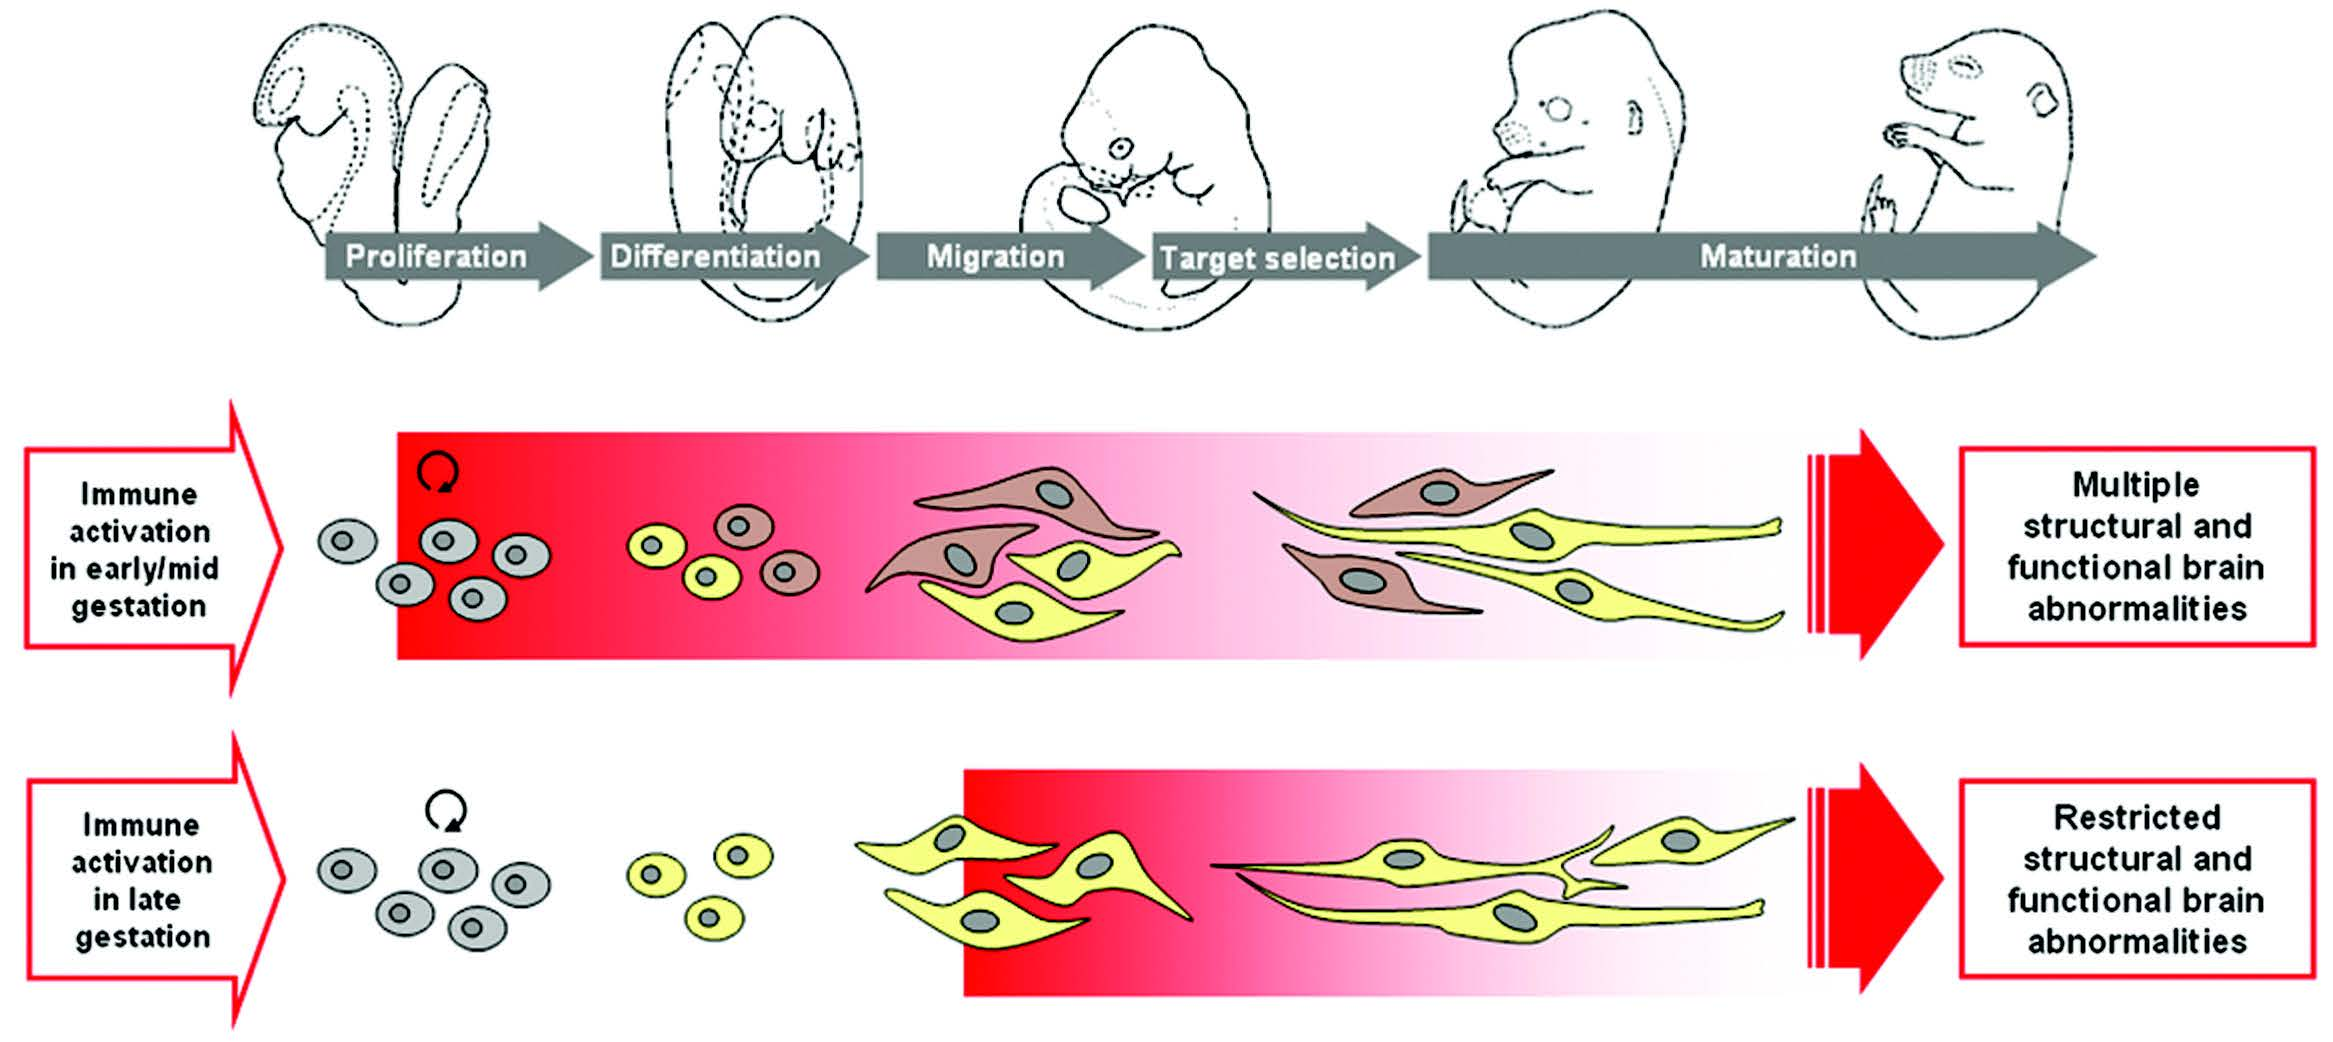
\includegraphics[width=\textwidth]{figure/mia_impact.jpg}
		\caption[Hypothesized model of the impact of prenatal immune challenge on fetal brain development]{Hypothesized model of the impact of prenatal immune challenge on fetal brain development.
			Maternal infection in early/mid pregnancy may affect early neurodevelopmental events in the fetal brain, thereby influencing the differentiation of neural precursor cells (grey) into particular neuronal phenotype (yellow or brown).
			This may predispose the developing fetal nervous system to additional failures leading to multiple structural and functional brain abnormalities in later life.
			Figure used with permission from Journal \citep{Meyer2007a}}
		\label{fig:miaEffect}
	\end{figure}
	
	On the other hand, an age dependent structural abnormalities in the mesoaccumbal and nigrostriatal dopamine systems were also found to be induced by \gls{mia} \citep{Vuillermot2010}.
	Specifically, \gls{mia} induces an early abnormality in specific dopaminergic systems such as those in the striatum and midbrian region \citep{Vuillermot2010}.
	Based on these observations, \citet{Meyer2007a} hypothesized that inflammation in the fetal brain during early gestation not only can disrupt neurodavelopmental processes such as cell proliferation and differentiation, it also predispose the developing nervous system to additional failures in subsequent cell migration, target selection, and synapse maturation (\cref{fig:miaEffect}) \citep{Meyer2007a}.
		
	In a separate study by \citet{Giovanoli2013}, mice were exposed to a lower dosage of \gls{polyic} during early gestation.
	A low dose of \gls{polyic} was selected as it only leads to restricted behavioral abnormalities in adulthood, thereby avoiding possible ceiling effects of the prenatal immunological manipulation on long-term brain and behavioral functions \citep{Giovanoli2013}. 
	Offspring born were then left undisturbed or exposed to unpredictable stress during peripubertal development.
	
	It was observed that offspring exposed to \gls{polyic} has an increased level of dopamine in the nucleus accumbens independent postnatal stress exposure.
	On the other hand, serotonin (5-HT) were decreased in the medial prefrontal cortex when exposed to postnatal stress regardless of prenatal exposure.
	Only when the offspring were exposed to both \gls{polyic} and postnatal stress will they have an increased dopamine levels in the hippocampus or will sensorimotor gating and psychotomimetic drug sensitivity be affected \citep{Giovanoli2013}.
	\citet{Giovanoli2013} therefore suggest that the prenatal insult serves as a ``disease primer'' that increase offspring's vulnerability to subsequent insults.
	
	Together, these results supports the involvement of \gls{mia} in the development of \glng{scz}.
	\citet{Brown2010} even estimated that one third of all \glng{scz} cases could have been prevented shall all infection were prevented from the entire pregnant population.
	
	One of the critical consideration in the study of \gls{mia} is the specific gestation period of vulnerability to infection-mediated disturbance \citep{Meyer2007a}.
	Early epidemiological studies have suggested that the second trimester of human pregnancy might be the vulnerability period.
	However, in birth cohorts such as the Prenatal Determinants of \Glng{scz}, it was found that the time window with maximum risk for infection-mediated disturbance in brain development is earlier than the second trimester of human pregnancy, can be as early as the first trimester \citep{Meyer2007a}.
	By reviewing existing \gls{mia} studies, \citet{Meyer2007a} suggested that effect of \gls{mia} during late pregnancy is restricted to the late developmental programmes, thus have a more restricted pathological phenotype in the grown offspring compared to \gls{mia} during early pregnancy \citep{Meyer2007a}.
	Subsequent \gls{mia} studies using the \gls{polyic} mouse model also support the hypothesis proposed by \citet{Meyer2007a}, where it was observed that \gls{mia} early in gestation event exert a more extensive impact on the phenotype of offspring \citep{Li2009c,Li2010a}.

	Despite the more severe impact of \gls{mia} during early gestation, most \gls{mia} studies have been focusing on the mid-gestation period.
	Therefore, there is a lack of understanding of the full molecular implication of early \gls{mia} events in adult brain.
	As technology advances, RNA Sequencing technique can now be employed to examine the global \gls{mrna} expression changes in the brain of the adult offspring exposed to \gls{mia} during early gestation.
	
	\subsection{RNA Sequencing}
	Before the development of the \gls{ngs}, the global expression changes can only be inspected by performing microarray analysis, which is based on probe hybridization.
	With the development of \gls{ngs} technology, sequencing can be performed on the \gls{mrna} fragments.
	
	When compared to microarray, RNA Sequencing has a number of advantages, most notably, because RNA Sequencing does not rely on specific probe hybridization, it does not suffer from bias introduced by probe performances such as signal saturation, cross-hybridization, background noises and non-specific hybridization \citep{Zhao2014}.
	
	Furthermore, in addition to differential expression analysis, alternative splicing analysis and de-novo transcript assembly can be readily performed on the same set of RNA Sequencing data.
	For microarray, de-novo assembly cannot be detected and specialized chips are required in order to perform alternative splicing analysis. 
	
	However, the analysis of RNA Sequencing is more complicated than microarray.
	The first consideration for the analysis of RNA Sequencing data is the sequence alignment.
	RNA sequencing generates sequence reads from the \gls{mrna} transcripts.
	Alignments have to be performed in order to quantify the expression level of the genes, where the sequence reads can either be aligned to the transcriptomes or the genome. 
		
	Sequence reads from RNA sequencing can be directly aligned to the transcriptomes as the reads are originated from the transcripts.
	However, multiple isoform can share the same exon. 
	This leads to problem of mapping uncertainties, e.g. a single read can be aligned to multiple transcripts \citep{Li2011e}.
	The alignment uncertainly will have a negative impact to downstream analysis. 
	
	Another alignment method is to align the reads directly to the genome. 
	However, as reads are originated from the \gls{mrna} transcripts, the intronic regions might be spliced out. 
	Therefore, the alignment algorithm will have to ``split'' the reads in order to align them onto the corresponding exons. 
	Some of the splice aware aligner includes TopHat2 \citep{Kim2013}, STAR \citep{Dobin2013} and MapSplice \citep{Wang2010}.
	
	Another difficulty in the analysis of RNA Sequencing data is the differential expression analysis. 
	In RNA Sequencing, the expression of a gene is represented by the number of reads aligned to the gene. 
	Differential expression analysis then aims to identify statistical significant difference in the gene expression level between different conditions. 
	However, unlike microarray, where the signal usually follows a normal distribution \citep{Hoyle2002,Giles2003}, the distribution of the RNA Sequencing count data are more complicated.
	
	Early RNA Sequencing experiment assumes the gene expression counts follows the Poisson distribution \citep{Marioni2008}, where the variance of the expression is expected to be equal to the mean of the expression.
	However, it was found that the assumption of Poisson distribution is too restrictive, as an over-dispersion was typically observed in RNA Sequencing data \citep{Anders2010}.
	Therefore, to overcome the problem of over-dispersion, differential expression analysis of RNA Sequencing data are required to model the expression using the negative binomial distribution \citep{Anders2010,Robinson2010} or the beta negative binomial distribution \citep{Trapnell2012}, instead of the Poisson distribution.

	\begin{figure}
		\centering
		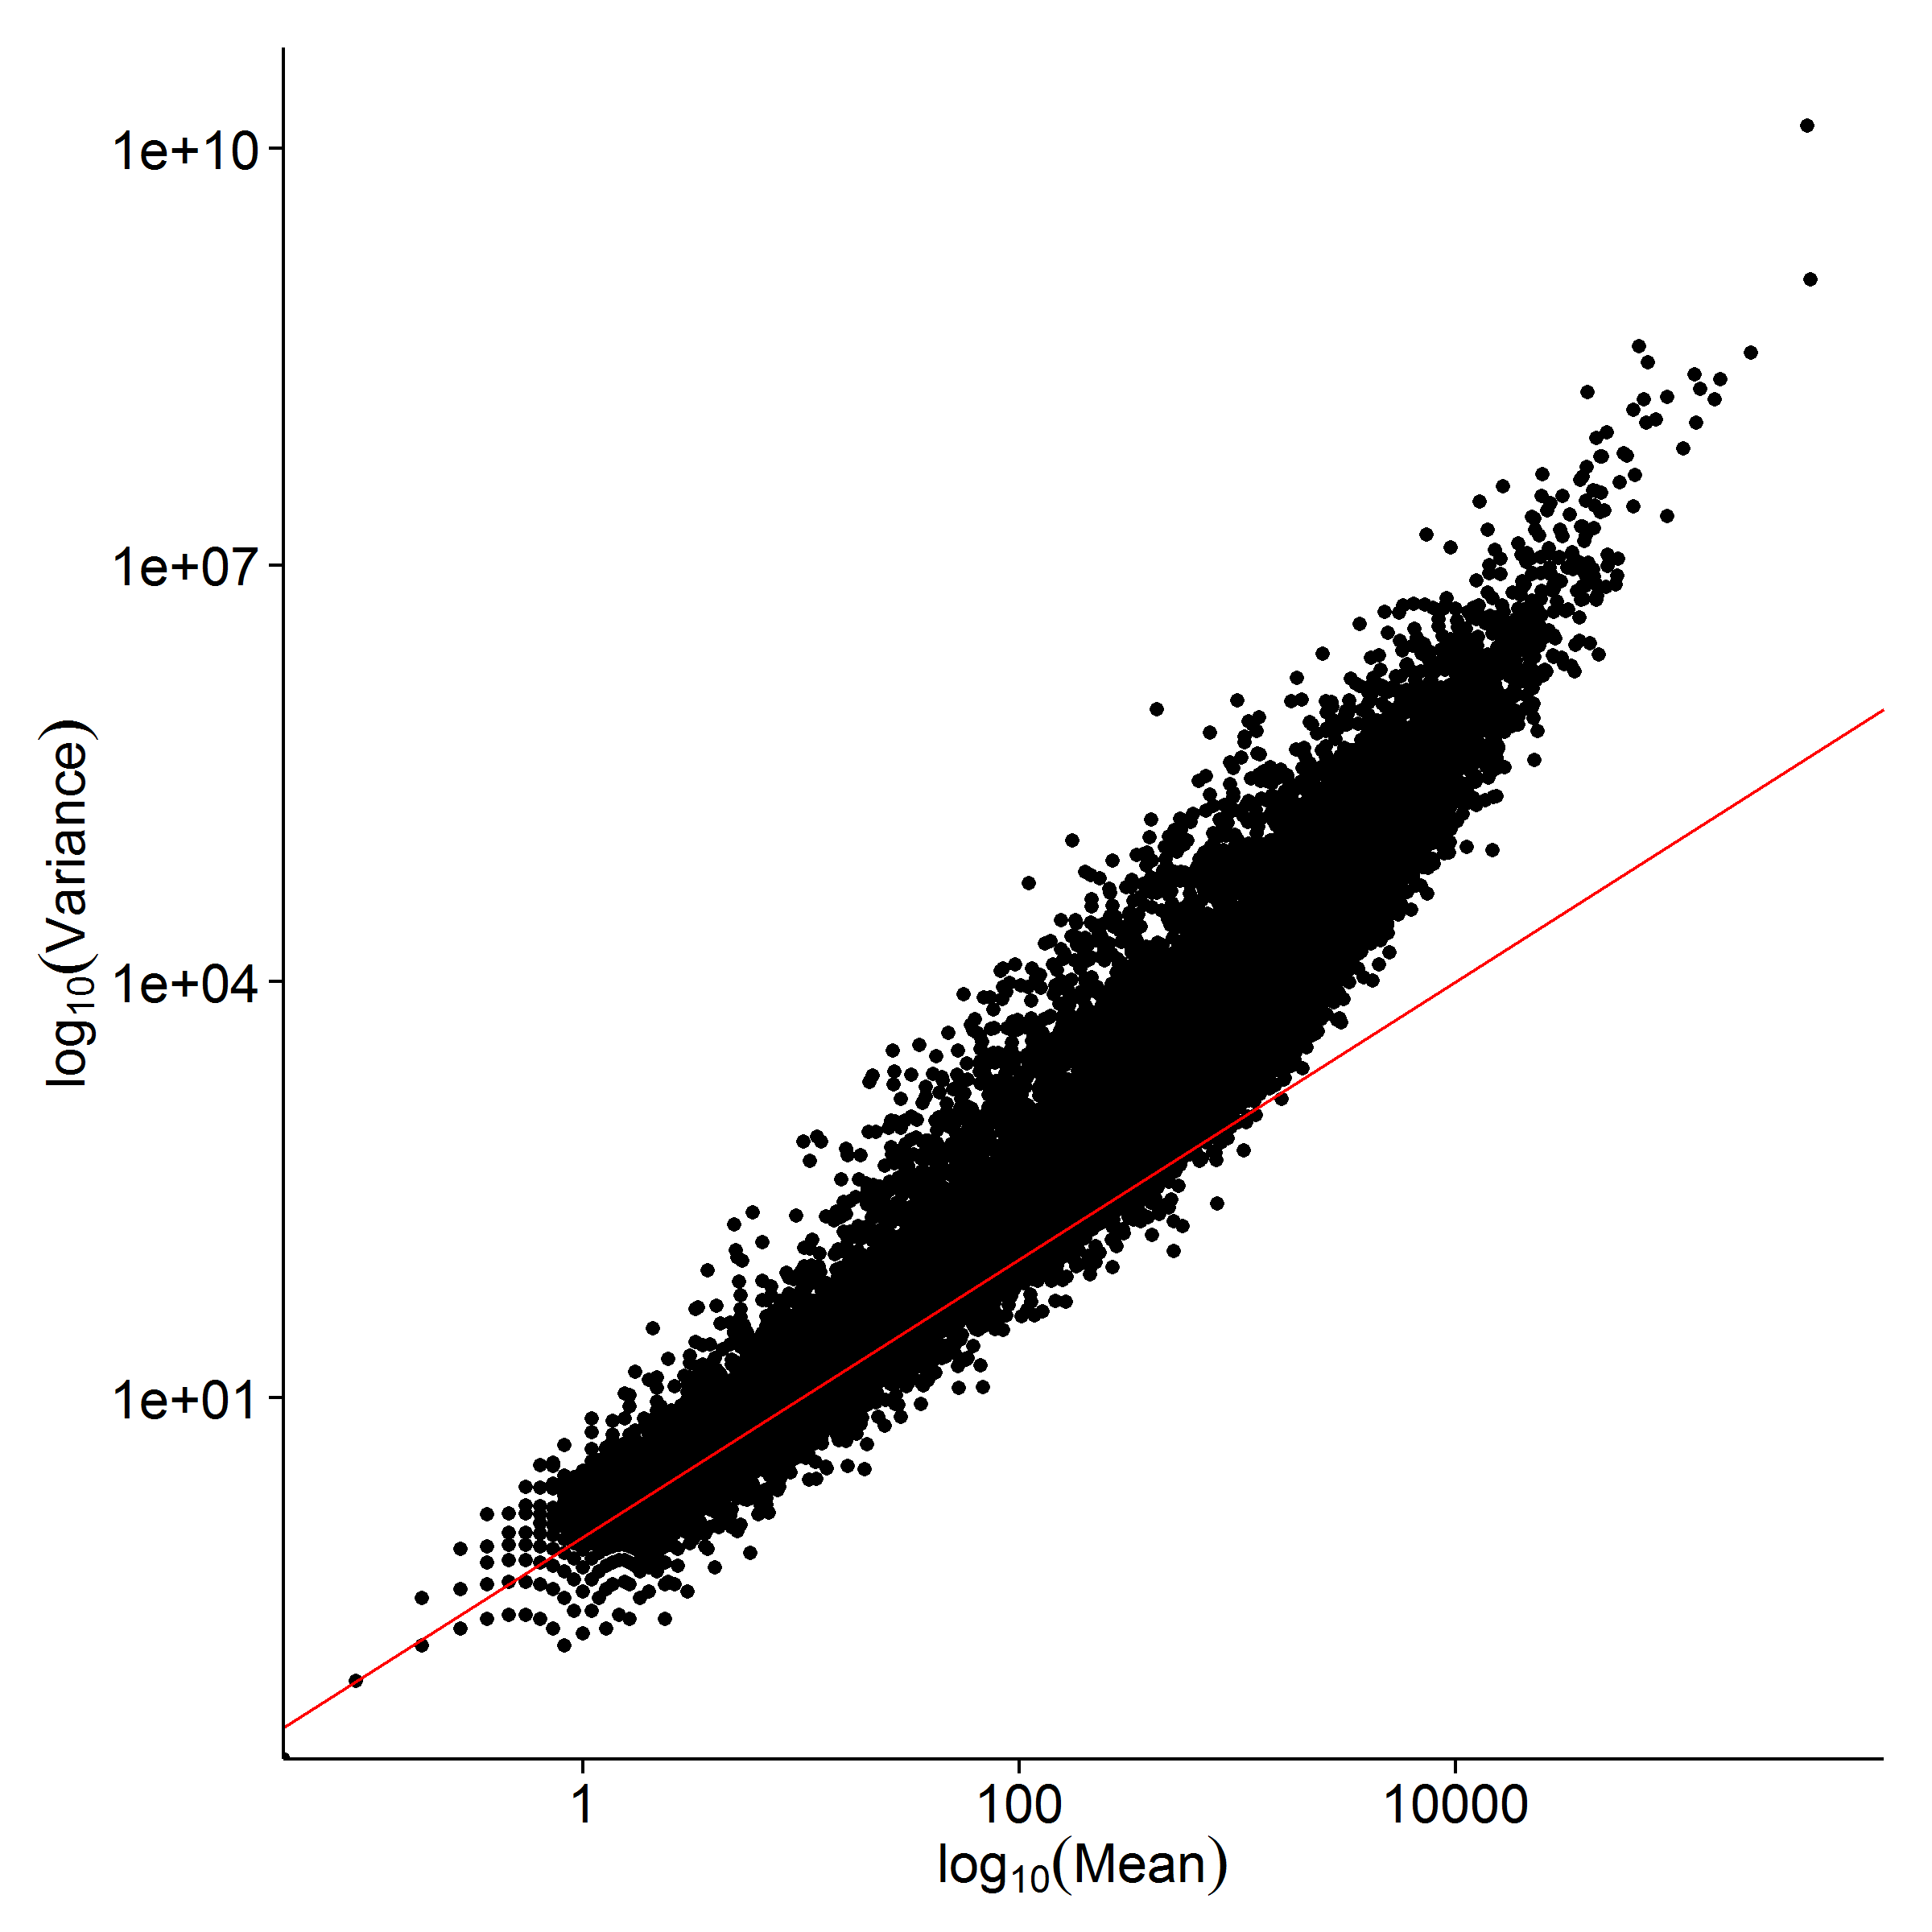
\includegraphics[width=0.5\textwidth]{figure/overdispersion.png}
		\caption[Over-dispersion observed in RNA Sequencing Count Data]{
			Over-dispersion observed in RNA Sequencing Count Data.
			If the RNA Sequencing count data follows the Poisson distribution, then the mean and variance of the data should be equal (follow the diagonal). 
			However, it was observed that as the mean increases, the variance increases even more, suggesting that there is an over-dispersion in the data. 
		}
	\end{figure}
	
	By using the appropriate aligner for the alignment of the RNA sequencing data, and using the appropriate statistical modeling, RNA Sequencing can provide unprecedented power for the analysis of expression changes.
	Therefore, RNA Sequencing might be an appropriate tool for the analysis of gene expression changes induced by \gls{mia} event.
	
	%TODO check till here
	\section{Summary}
	In this thesis, we would like to perform extensive simulations to investigate the effect of different genetic architectures and sampling strategies in \gls{GWAS} to the performance of \gls{ldsc}, for example, the effect of extreme phenotype samplings.
	On the other hand, as \gls{ldsc} might under-perform in certain scenarios (e.g. oligogenic traits) \citep{Bulik-Sullivan2015}, there is a need of developing an alternative algorithm that can be applied for various genetic architecture models with equal performance.
	Thus we developed an alternative algorithm for the estimation of \gls{SNP} heritability using summary statistics from \gls{GWAS}.
	Ultimately, we would like to re-estimate the \gls{SNP} heritability of \glng{scz}.

	Currently, evidences suggest there might be an interaction between prenatal infection and genetic variations in the development of \glng{scz} \citep{Tienari2004,Clarke2009}.
	Therefore, we hypothesize that the differential gene expression induced by \gls{mia} and genetic mutation might be acting upon the same functional pathways/gene sets.
	To test our hypothesis, a RNA Sequencing study was performed to capture gene expression changes induced by early \gls{mia} events (\gls{gd}9) in the mouse cerebellum using the \gls{polyic} mouse model.
	Enrichment analysis was then performed to investigate whether the differential expressed genes were enriched in gene sets associated with \glng{scz}.
	Partitioning of heritability were also performed to investigate whether these gene sets contribute disproportionately to the \gls{SNP} heritability of \glng{scz}.
	
	Furthermore, recent study from our lab suggested that n-3 \gls{pufa} rich diet might help to reduce the \glng{scz}-like behaviour in mice exposed to early \gls{mia} insults \citep{Li2015}.
	Therefore, we also investigated the effect of n-3 \gls{pufa} rich diet in the gene expression pattern in the brain of the \gls{mia} samples. 
	
	To summarize, this thesis will be divided into three parts. 
	The main focus of \Cref{heritabilityChapter} is to investigate the effect of different sampling strategies and genetic architecture to the performance of \gls{ldsc}.
	At the same time, \gls{shrek}, an alternative algorithm for the estimation of \gls{SNP} heritability is also introduced. 
	We also re-examined the \gls{SNP} heritability of \glng{scz} and other psychiatric disorders.
	
	\Cref{omegaProject} describes our the RNA sequencing study on the effect of \gls{mia} and n-3 \gls{pufa} diet on gene expression of the mouse cerebellum. 

	
	Lastly, we summarize and conclude all findings in \Cref{conclusionChapter} and give future perspectives on genetic studies of \glng{scz}.
	
	\chapter{Heritability Estimation}

% Need to stress that we are only calculating the narrow sense heritability
	\section{Introduction}
	The development of \glng{ldsc} has brought great prospect in estimating the heritability of complex disease for one can now estimate the heritability of a trait without requiring the rare genotype. 
	However, as noted by the author of \gls{ldsc}, when the number of causal variants were small, or when working on targeted genotype array, \gls{ldsc} tends to have a larger standard error or might produce funky results\citep{Bulik-Sullivan2015}.
	Ideally, we would like to be able to robustly estimate the heritability for all traits, disregarding the genetic architecture (e.g. number of causal \glspl{SNP}).
	
	On the other hand, it has been shown that there can be huge bias in the heritability estimation of \gls{gcta} when prevalence of a dichotomous trait is low\citep{Golan2014}.
	Although \citet{Golan2014} developed the \gls{pcgc}, which can provide robust estimation of heritability for traits with different prevalence, it still relies on the relationship matrix and therefore require the raw genotype of the samples. 
	
	Herein, we would like to develop an alternative algorithm to \gls{ldsc} for heritability estimation using only the test statistics. 
	We would also like to inspect whether if \gls{ldsc}'s heritability estimation is robust to prevalence of a trait. 
	A number of simulations were performed to compare the performance of \gls{ldsc} and our algorithm under different conditions.
	
	The work in this chapter were done in collaboration with my colleagues who have kindly provide their support and knowledges to make this piece of work possible.
	Dr Johnny Kwan, Dr Miaxin Li and Professor Sham have helped to laid the framework of this study. 
	Dr Timothy Mak has derived the mathematical proof for our heritability estimation method. 
	Miss Yiming Li, Dr Johnny Kwan, Dr Miaxin Li, Dr Timothy Mak and Professor Sham have helped with the derivation of the standard error of the heritability estimation. 
	Dr Henry Leung has provided critical suggestions on the implementation of the algorithm.
	
	\section{Methodology}	
		The overall aims of this study is to develop a robust algorithm for the estimation of the narrow sense heritability using only the summary statistic from a \gls{GWAS}.
		In \gls{GWAS}, the test statistic of a particular \gls{SNP} should be proportional to its effect size and the effect size from all the other \glspl{SNP} in \gls{LD} with it.
		Based on this property, we may use the information from the \gls{LD} matrix and the test statistic of the \gls{GWAS} \gls{SNP} the estimate the narrow sense heritability.
		
		
		\subsection{Heritability Estimation}
			Remember that the narrow-sense heritability is defined as 
			$$
				h^2 = \frac{\mathrm{Var}(X)}{\mathrm{Var}(Y)}
			$$
			where $\mathrm{Var}(X)$ is the variance of the genotype and $\mathrm{Var}r(Y)$ is the variance of the phenotype.
			In a \gls{GWAS}, regression were performed between the \glspl{SNP} and the phenotypes, giving
			\begin{equation}
				Y=\beta X+\epsilon
				\label{eq:standardRegress}
			\end{equation}
			where $Y$ and $X$ are the standardized phenotype and genotype respectively. 
			$\epsilon$ is then the error term, accounting for the non-genetic elements contributing to the phenotype (e.g. Environment factors).
			Based on \cref{eq:standardRegress}, one can then have
			\begin{align}
				\mathrm{Var}(Y) = \mathrm{Var}(\beta X)+ \mathrm{Var}(\epsilon) \nonumber\\
				\mathrm{Var}(Y) = \beta^\mathrm{Var}(X) \nonumber\\
				\beta^2\frac{\mathrm{Var}(X)}{\mathrm{Var}(Y)}= 1
				\label{eq:betaHeri}
			\end{align}
			$\beta^2$ is then considered as the portion of phenotype variance explained by the variance of genotype, which can also be considered as the narrow-sense heritability of the phenotype.
					
			A challenge in calculating the heritability from \gls{GWAS} data is that usually only the test-statistic or p-value were provided and one will not be able to directly calculate the heritability based on \cref{eq:betaHeri}. 
			In order to estimation the heritability of a trait from the \gls{GWAS} test-statistic, we first observed that when both $X$ and $Y$ are standardized, $\beta^2$ will be equal to the coefficient of determination ($r^2$). 
			Then, based on properties of the Pearson product-moment correlation coefficient:
			\begin{equation}
				r = \frac{t}{\sqrt{n-2+t^2}}
				\label{eq:pearsonProduct}
			\end{equation}
			where $t$ follows the student-t distribution and $n$ is the number of samples, one can then obtain the $r^2$ by taking the square of \cref{eq:pearsonProduct}
			\begin{equation}
				r^2 = \frac{t^2}{n-2+t^2}
				\label{eq:oriRSquared}
			\end{equation}
			It is observed that $t^2$ will follow the F-distribution.
			When $n$ is big, $t^2$ will converge into $\chi^2$ distribution.
			
			Furthermore, when the effect size is small and $n$ is big, $r^2$ will be approximately $\chi^2$ distributed with mean $\sim 1$. 
			We can then approximate \cref{eq:oriRSquared} as
			\begin{equation}
				r^2= \frac{\chi^2}{n}
				\label{eq:approxChi}
			\end{equation}
			and define the \emph{observed} effect size of each \gls{SNP} to be
			\begin{equation}
			f=\frac{\chi^2-1}{n}
			\label{eq:observedEffect}
			\end{equation}
			
			When there are \gls{LD} between each individual \glspl{SNP}, the situation will become more complicated as each \glspl{SNP}' observed effect will contains effect coming from other \glspl{SNP} in \gls{LD} with it:
			\begin{equation}
			f_{observed} = f_{true}+f_{LD}
			\label{eq:conceptF}
			\end{equation}
			
			To account for the \gls{LD} structure, we first assume our phenotype $\boldsymbol{Y}$ and genotype $\boldsymbol{X}=(X_1,X_2,\dots,X_m)^t$ are standardized and that
			\begin{align*}
				\boldsymbol{Y}\sim f(0,1) \\
				\boldsymbol{X}\sim f(0,\boldsymbol{R})
			\end{align*}
			Where $\boldsymbol{R}$ is the \gls{LD} matrix between \glspl{SNP}.
			
			We can then express \cref{eq:standardRegress} in matrix form:
			\begin{align}
				\boldsymbol{Y}=\boldsymbol{\beta}^t\boldsymbol{X}+\epsilon
				\label{eq:matrixRegress}
			\end{align}
			Because the phenotype is standardized with variance of 1, the narrow sense heritability can then be expressed as
			\begin{align}
				Heritability& = \frac{\mathrm{Var}(\boldsymbol{\beta}^t\boldsymbol{X})}{\mathrm{Var}(\boldsymbol{Y})} \nonumber\\
				&=\mathrm{Var}(\boldsymbol{\beta}^t\boldsymbol{X})
			\end{align}
			If we then assume now that $\boldsymbol{\beta} = (\beta_1, \beta_2,\dots,\beta_m)^t$ has distribution
			\begin{align*}
				\boldsymbol{\beta}&\sim f(0,\boldmath{H})\\
				\boldsymbol{H}&=diag(\boldsymbol{h})\\
				\boldsymbol{h}&=(h_1^2,h_2^2,\dots,h_m^2)^t
			\end{align*}
			where $\boldsymbol{H}$ is the variance of the ``true'' effect. 
			It is shown that heritability can be expressed as %The later part was gone because that will contains E(\beta) which = 0
			\begin{align}
			\mathrm{Var}(\boldsymbol{\beta}^t\boldsymbol{X}) &= \mathrm{E}_X\mathrm{Var}_{\beta|X}(\boldsymbol{X}^t\boldsymbol{\beta})+\mathrm{Var}_X\mathrm{E}_{(\beta|X)}(\boldsymbol{\beta}^2\boldsymbol{X}) \nonumber\\
			&=\mathrm{E}_X(\boldsymbol{X}^t\boldsymbol{\beta\beta}^T\boldsymbol{X}) \nonumber\\ 
			&= \mathrm{E}_X(\boldsymbol{X}^t\boldsymbol{HX}) \nonumber\\
			&= \mathrm{E}(\boldsymbol{X})^t\boldsymbol{H}\mathrm{E}(\boldsymbol{X})+\mathrm{Tr}(\mathrm{Var}(\boldsymbol{X}\boldsymbol{H})) \nonumber\\
			&=\mathrm{Tr}(\mathrm{Var}(\boldsymbol{X}\boldsymbol{H})) \nonumber\\
			&=\sum_ih_i^2
			\label{eq:proveHerit}
			\end{align}
			
			Now if we consider the covariance between \gls{SNP} i ($\boldsymbol{X_i}$) and $\boldsymbol{Y}$, we have
			\begin{align}
			 \mathrm{Cov}(\boldsymbol{X}_i,\boldsymbol{Y}) &= \mathrm{Cov}(\boldsymbol{X}_i,\boldsymbol{\beta}^t\boldsymbol{X}+\epsilon) \nonumber\\
			 &=\mathrm{Cov}(\boldsymbol{X}_i,\boldsymbol{\beta}^t\boldsymbol{X}) \nonumber\\
			 &=\sum_j{\mathrm{Cov}(\boldsymbol{X}_i,\boldsymbol{X}_j)\boldsymbol{\beta}_j} \nonumber\\
			 &=\boldsymbol{R}_i\boldsymbol{\beta}_j
			 \label{eq:covPhenoTrue}
			\end{align}
			
			As both $\boldsymbol{X}$ and $\boldsymbol{Y}$ are standardized, the covariance will equal to the correlation and we can define the correlation between \gls{SNP} i and $Y$ as
			\begin{equation}
				\rho_i = \boldsymbol{R}_i\boldsymbol{\beta}_j
				\label{eq:corPhenoTrue}
			\end{equation}
			In reality, the \emph{observed} correlation usually contains error. 
			Therefore we define the \emph{observed} correlation between SNP$_i$ and the phenotype($\hat{\rho_i}$) to be
			\begin{equation}
			\hat{\rho_i} = \rho_i+\frac{\epsilon_i}{\sqrt{n}}
			\label{eq:obsPheno}
			\end{equation}
			for some error $\epsilon_i$. 
			The distribution of the correlation coefficient about the true correlation $\rho$ is approximately
			$$
				\hat{\rho_i}\sim f(\rho_i, \frac{(1-\rho^2)^2}{n})
			$$
			By making the assumption that $\rho_i$ is close to 0 for all $i$, we have 
			\begin{align*}
				\mathrm{E}(\epsilon_i|\rho_i)&\sim 0\\
				\mathrm{Var}(\epsilon_i|\rho_i)&\sim 1
			\end{align*}
			We then define our $z$-statistic and $\chi^2$-statistic as
			\begin{align*}
				z_i &= \hat{\rho_i}\sqrt{n} \\
				\chi^2 &= z_i^2\\
				&=\hat{\rho_i}^2n
			\end{align*}
			From \cref{eq:obsPheno} and \cref{eq:corPhenoTrue}, $\chi^2$ can then be expressed as
			\begin{align*}
			\chi^2&=\hat{\rho}^2n\\
			&=n(\boldsymbol{R}_i\boldsymbol{\beta}_j+\frac{\epsilon_i}{\sqrt{n}})^2
			\end{align*}
			The expectation of $\chi^2$ is then
			\begin{align*}
			\mathrm{E}(\chi^2) &= n(\boldsymbol{R}_i\boldsymbol{\beta\beta}^t\boldsymbol{R}_i+2\boldsymbol{R}_i\boldsymbol{\beta}\frac{\epsilon_i}{\sqrt{n}}+\frac{\epsilon_i^2}{n}) \\
			&= n\boldsymbol{R}_i\boldsymbol{H}\boldsymbol{R}_i+1
			\end{align*}
			To derive least square estimates of $h_i^2$, we need to find $\hat{h_i^2}$ which minimizes
			\begin{align*}
				\sum_i(\chi_i^2-\mathrm{E}(\chi_i^2))^2&=\sum_i(\chi_i^2-(n\boldsymbol{R}_i\boldsymbol{H}\boldsymbol{R}_i+1))^2 \\
				&=\sum_i(\chi_i^2-1-n\boldsymbol{R}_i\boldsymbol{H}\boldsymbol{R}_i)^2 
			\end{align*}
			If we define 
			\begin{equation}
			f_i= \frac{\chi_i^2-1}{n}
			\label{eq:defineF}
			\end{equation}
			we got
			\begin{align}
			\sum_i(\chi_i^2-\mathrm{E}(\chi_i^2))^2&=\sum_i(f_i-\boldsymbol{R}_i\boldsymbol{H}\boldsymbol{R}_i)^2 \nonumber\\
			&=\boldsymbol{ff}^t-2\boldsymbol{f}^t\boldsymbol{R_{sq}\hat{h}}+\boldsymbol{\hat{h}}^t\boldsymbol{R_{sq}}^t\boldsymbol{R_{sq}\hat{h}}
			\label{eq:leastSquareH}
			\end{align}
			where $\boldsymbol{R_{sq}} = \boldsymbol{R}\circ\boldsymbol{R}$.
			By differentiating \cref{eq:leastSquareH} w.r.t $\hat{h}$ and set to 0, we get
			\begin{align}
				2\boldsymbol{R_{sq}}^t\boldsymbol{R_{sq}}\boldsymbol{\hat{h^2}}-2\boldsymbol{R_{sq}f}&=0 \nonumber\\
				\boldsymbol{R_{sq}}\boldsymbol{\hat{h^2}} &=\boldsymbol{f}
				\label{eq:shrekEq}
			\end{align}
			And the heritability is then defined as 
			\begin{equation}
			\hat{Heritability} = \boldsymbol{1}^t\boldsymbol{R_{sq}}^{-1}\boldsymbol{f}
			\label{eq:fullShrek}
			\end{equation}
		\subsection{Calculating the \Glng{se}}
			From \cref{eq:fullShrek}, we can derive the variance of heritability $H$ as 
			\begin{align}
				\mathrm{Var}(H) &= \mathrm{E}[H^2]-\mathrm{E}[H]^2\nonumber\\
				&=\mathrm{E}[(\boldsymbol{1}^t\boldsymbol{R_{sq}}^{-1}\boldsymbol{f})^2]-\mathrm{E}[\boldsymbol{1}^t\boldsymbol{R_{sq}}^{-1}\boldsymbol{f}](\mathrm{E}[\boldsymbol{1}^t\boldsymbol{R_{sq}}^{-1}\boldsymbol{f}])^t \nonumber \\
				&=\mathrm{E}[\boldsymbol{1}^t\boldsymbol{R_{sq}}^{-1}\boldsymbol{ff}^t\boldsymbol{R_{sq}}^{-1}\boldsymbol{1}]-\mathrm{E}[\boldsymbol{1}^t\boldsymbol{R_{sq}}^{-1}\boldsymbol{f}](\mathrm{E}[\boldsymbol{1}^t\boldsymbol{R_{sq}}^{-1}\boldsymbol{f}])^t \nonumber \\
				&=\boldsymbol{1}^t\boldsymbol{R_{sq}}^{-1}\mathrm{E}[\boldsymbol{ff}^t]\boldsymbol{R_{sq}}^{-1}\boldsymbol{1}-\mathrm{E}[\boldsymbol{1}^t\boldsymbol{R_{sq}}^{-1}\boldsymbol{f}](\mathrm{E}[\boldsymbol{1}^t\boldsymbol{R_{sq}}^{-1}\boldsymbol{f}])^t \nonumber \\
				&=\boldsymbol{1}^t\boldsymbol{R_{sq}}^{-1}\mathrm{Var}(\boldsymbol{f})\boldsymbol{R_{sq}}^{-1}\boldsymbol{1}+\mathrm{E}[\boldsymbol{1}^t\boldsymbol{R_{sq}}^{-1}\boldsymbol{f}](\mathrm{E}[\boldsymbol{1}^t\boldsymbol{R_{sq}}^{-1}\boldsymbol{f}])^t-\mathrm{E}[\boldsymbol{1}^t\boldsymbol{R_{sq}}^{-1}\boldsymbol{f}](\mathrm{E}[\boldsymbol{1}^t\boldsymbol{R_{sq}}^{-1}\boldsymbol{f}])^t \nonumber\\
				&=\boldsymbol{1}^t\boldsymbol{R_{sq}}^{-1}\mathrm{Var}(\boldsymbol{f})\boldsymbol{R_{sq}}^{-1}\boldsymbol{1}
				\label{eq:varHvarf}
			\end{align}
			Therefore, to obtain the variance of $H$, we first need to calculate the variance covariance matrix of $\boldsymbol{f}$.
			
			We first consider the standardized genotype $X_i$ with standard normal mean $z_i$ and non-centrality parameter
			$\mu_i$, we have
			\begin{align*}
				\mathrm{E}[X_i]&=\mathrm{E}[z_i+\mu_i]\\
				&=\mu_i\\
				\mathrm{Var}(X_i) &=\mathrm{E}[(z_i+\mu_i)^2]+\mathrm{E}[(z_i+\mu_i)]^2\\
				&=\mathrm{E}[z_i^2+\mu_i^2+2z_i\mu_i]+\mu_i^2\\
				&=1 \\
				\mathrm{Cov}(X_i,X_j)&=\mathrm{E}[(z_i+\mu_i)(z_j+\mu_j)]-\mathrm{E}[z_i+\mu_i]\mathrm{E}[z_j+\mu_j]\\
				&=\mathrm{E}[z_iz_j+z_i\mu_j+\mu_iz_j+\mu_i\mu_j]-\mu_i\mu_j\\
				&=\mathrm{E}[z_iz_j]+\mathrm{E}[z_i\mu_j]+\mathrm{E}[z_j\mu_i]+\mathrm{E}[\mu_i\mu_j]-\mu_i\mu_j\\
				&=\mathrm{E}[z_iz_j]
			\end{align*}
			As the genotypes are standardized, therefore $\mathrm{Cov}(X_i,X_j)==\mathrm{Cor}(X_i,X_j)$, we can obtain
			$$
				\mathrm{Cov}(X_i,X_j)=\mathrm{E}[z_iz_j]=R_{ij}
			$$
			where $R_{ij}$ is the \gls{LD} between \gls{SNP}$_i$ and \gls{SNP}$_j$.
			Given these information, we can then calculate $\mathrm{Cov}(\chi_i^2,\chi_j^2)$ as:
			\begin{align*}
				\mathrm{Cov}(X_i^2,X_j^2)=&\mathrm{E}[(z_i+\mu_i)^2(z_j+\mu_j)^2]-\mathrm{E}[z_i+\mu_i]\mathrm{E}[z_j+\mu_j]\\
				=&\mathrm{E}[(z_i^2+\mu_i^2+2z_i\mu_i)(z_j^2+\mu_j^2+2z_j\mu_j)] \\
				&-\mathrm{E}[z_i^2+\mu_i^2+2z_i\mu_i]\mathrm{E}[z_j^2+\mu_j^2+2z_j\mu_j]\\
				=&\mathrm{E}[(z_i^2+\mu_i^2+2z_i\mu_i)(z_j^2+\mu_j^2+2z_j\mu_j)]\\
				&-(\mathrm{E}[z_i^2]+\mathrm{E}[\mu_i^2]+2\mathrm{E}[z_i\mu_i])(\mathrm{E}[z_j^2]+\mathrm{E}[\mu_j^2]+2\mathrm{E}[z_j\mu_j])\\
				=&\mathrm{E}[z_i^2(z_j^2+\mu_j^2+2z_j\mu_j)+\mu_i^2(z_j^2+\mu_j^2+2z_j\mu_j)+2z_i\mu_i(z_j^2+\mu_j^2+2z_j\mu_j)]\\
				&-(1+\mu_i^2)(1+\mu_j^2)\\
				=&\mathrm{E}[z_i^2(z_j^2+\mu_j^2+2z_j\mu_j)]+\mu_i^2\mathrm{E}[z_j^2+\mu_j^2+2z_j\mu_j]\\
				&+2\mu_i\mathrm{E}[z_i(z_j^2+\mu_j^2+2z_j\mu_j)]-(1+\mu_i^2)(1+\mu_j^2)\\
				=&\mathrm{E}[z_i^2z_j^2+z_i^2\mu_j^2+2z_i^2z_j\mu_j]+\mu_i^2+\mu_i^2\mu_j^2\\
				&+2\mu_i\mathrm{E}[z_iz_j^2+z_i\mu_j^2+2z_iz_j\mu_j]-(1+\mu_i^2)(1+\mu_j^2)\\
				=&\mathrm{E}[z_i^2z_j^2]+\mu_j^2+\mu_i^2+\mu_i^2\mu_j^2+4\mu_i\mu_j\mathrm{E}[z_iz_j]-(1+\mu_i^2+\mu_j^2+\mu_i\mu_j)\\
				=&\mathrm{E}[z_i^2z_j^2]+4\mu_i\mu_j\mathrm{E}[z_iz_j]-1
			\end{align*}
			Remember that $\mathrm{E}[z_iz_j] = R_{ij}$, we then have
			$$
				\mathrm{Cov}(X_i^2, X_j^2)=\mathrm{E}[z_i^2z_j^2]+4\mu_i\mu_jR_{ij}-1
			$$
			By definition, 
			$$
				z_i|z_j\sim N(\mu_i+R_{ij}(z_j-\mu_j),1-R_{ij}^2)
			$$
			We can then calculate $\mathrm{E}[z_i^2z_j^2]$ as
			\begin{align*}
				\mathrm{E}[z_i^2z_j^2]&=\mathrm{Var}[z_iz_j]+\mathrm{E}[z_iz_j]^2\\
				&=\mathrm{E}[\mathrm{Var}(z_iz_j|z_i)]+\mathrm{Var}[\mathrm{E}[z_iz_j|z_i]]+R_{ij}^2\\
				&=\mathrm{E}[z_j^2\mathrm{Var}(z_i|z_j)]+\mathrm{Var}[z_j\mathrm{E}[z_i|z_j]]+R_{ij}^2\\
				&=(1-R_{ij}^2)\mathrm{E}[z_j^2]+\mathrm{Var}(z_j(\mu_i+R_{ij}(z_j-\mu_j)))+R_{ij}^2\\
				&=(1-R_{ij}^2)+\mathrm{Var}(z_j\mu_i+R_{ij}z_j^2-\mu_jz_jR_{ij})+R_{ij}^2\\
				&=1+\mu_i^2\mathrm{Var}(z_j)+R_{ij}^2\mathrm{Var}(z_j^2)-\mu_j^2R_{ij}^2\mathrm{Var}(z_j)\\
				&=1+2R_{ij}^2
			\end{align*}
			As a result, the variance covariance matrix of the $\chi^2$ variances represented as
			\begin{equation}
				\mathrm{Cov}(X_i^2,X_j^2) = 2R_{ij}^2+4R_{ij}\mu_i\mu_j
				\label{eq:finalChi}
			\end{equation}
			As we only have the \emph{observed} expectation, we should re-define \cref{eq:finalChi} as
			\begin{equation}
				\mathrm{Cov}(X_i^2,X_j^2) = \frac{2R_{ij}^2+4R_{ij}\mu_i\mu_j}{n^2}
				\label{eq:finalChiCov}
			\end{equation}
			where $n$ is the sample size.
			
			By substituting \cref{eq:finalChiCov} into \cref{eq:varHvarf}, we will get
			\begin{align}
				\mathrm{Var}(H) &=\boldsymbol{1}^t\boldsymbol{R_{sq}}^{-1}\frac{2\boldsymbol{R_{sq}}+4\boldsymbol{R}\circ \boldsymbol{zz}^t}{n^2}\boldsymbol{R_{sq}}^{-1}\boldsymbol{1}
				\label{eq:covH}
			\end{align}
			where $\boldsymbol{z} = \sqrt{\boldsymbol{\chi^2}}$ from \cref{eq:defineF}, with the direction of effect as its sign and $\circ$ is the element-wise product (Hadamard product).
			 
			The problem with \cref{eq:covH} is that it requires the direction of effect. 
			Without the direction of effect, the estimation of \gls{se} will be inaccurate. 
			If we consider that $\boldsymbol{f}$ is approximately $\chi^2$ distributed, we might view \cref{eq:shrekEq} as a decomposition of a vector of $\chi^2$ distributions with degree of freedom of 1. 
			Replacing the vector $\boldsymbol{f}$ with a vector of 1, we can perform the decomposition of the degree of freedom, getting the ``effective number''($e$) of the association\citep{Li2011}. 
			%The problem of this effective number is that they uses the eigenvalue instead of this multiplication.
			%So either we have to explain why we don't follow it (therefore explaining the slidding windows) or we should just avoid mentioning the effective number
			Substituting $e$ into the variance equation of non-central $\chi^2$ distribution will yield
			\begin{equation}
			\mathrm{Var}(H) = \frac{2(e+2H)}{n^2}
			\label{eq:effectiveChi}
			\end{equation}
			\cref{eq:effectiveChi} should in theory gives us an heuristic estimation of the \gls{se}. 
			Moreover, the direction of effect was not required for \cref{eq:effectiveChi}, reducing the number of input required from the user.
		\subsection{Case Control Studies}	 
		%Discuss on the liability threshold model. Then the apply orange paper. Then explain how to get the results. 
			When dealing with case control data, as the phenotype were usually discontinuous, we cannot directly use \cref{eq:fullShrek} to estimate the heritability.
			Instead, we will need to employ the concept of liability threshold model from \cref{sec:liability}. 
			
			Based on the derivation of \citet{Yang2010}, the approximate ratio between the \gls{ncp} obtained from case control studies ($NPC_{CC}$) and quantitative trait studies($NCP_{QT}$) were
		
			\begin{equation}
			\frac{NCP_{CC}}{NCP_{QT}} = \frac{i^2v(1-v)N_{CC}}{(1-K)^2N_{QT}}
			\label{eq:originNCPTransform}
			\end{equation}
			where
			\begin{align*}
			 K &= \text{Population Prevalence} \\
			 v &= \text{Proportion of Cases}\\
			 N &= \text{Total Number of Samples}\\
			 i &= \frac{z}{K}\\
			 z &= \text{height of standard normal curve at truncation pretained to K}
			\end{align*}
			
			Using this approximation deviated by \citet{Yang2010}, we can directly transform the \gls{ncp} between the case control studies and quantitative trait studies.
			As we were transforming the \gls{ncp} of a single study, the $N_{CC}$ and $N_{QT}$ will be the same, therefore \cref{eq:originNCPTransform} became
			\begin{equation}
			NCP_{QT} = \frac{NCP_{CC}(1-K)^2}{i^2v(1-v)}
			\label{eq:transform}
			\end{equation}
			
			By combining \cref{eq:transform} and \cref{eq:defineF}, we can then have
			\begin{equation}
			f = \frac{(\chi^2_{CC}-1)(1-K)^2}{ni^2v(1-v)}
			\end{equation}
			where $\chi^2_{CC}$ is the test statistic from the case control association test.
			Finally, the heritability estimation of case control studies can be simplified to 
			\begin{equation}
			\hat{Heritability} =\frac{(1-K)^2}{i^2v(1-v)} \boldsymbol{1}^t\boldsymbol{R_{sq}}^{-1}\boldsymbol{f}
			\label{eq:caseControlHerit}
			\end{equation}
			
		\subsection{Extreme Phenotype Selections}
			%Explain why we perform extreme phenotype selections. Explain how that affect the variance of the estimation. Finally, explain how to perform heritability estimation on extreme phenotype. 
			When extreme phenotype selection were performed, the variance of the selected phenotype will not be representative of that in the population.
			Most notably, the variance of the post selection phenotype will tends to increase.
			Thus, to adjust for this bias, one can multiple the estimated heritability $\hat{h^2}$ by the ratio between the variance before $V_P$ and after $V_{P'}$ the selection process\citep{Sham2014}:
			
			\begin{equation}
			\hat{Heritability} = \frac{V_{P'}}{V_P}\boldsymbol{1}^t\boldsymbol{R_{sq}}^{-1}\boldsymbol{f}
			\label{eq:extremeShrek}
			\end{equation}
			
		\subsection{Calculating the \glsentrylong{LD} matrix}
			% Might want to remove this section as we no longer use this correction
			To estimate the heritability, the population \gls{LD} matrix is required.
			In reality, one can only obtain the \gls{LD} matrix based on a subset of the population (e.g. the 1000 genome project\citep{Project2012} or the HapMap project\citep{Altshuler2010}).
			There are therefore sampling errors among the \gls{LD} elements. 
			
			Now if we consider \cref{eq:fullShrek}, the $\boldsymbol{R_{sq}}$ matrix is required.
			As the squared \gls{LD} is used, a positive bias is induced into our $\boldsymbol{R_{sq}}$ matrix. 
			
			Based on \citet{Shieh2010}, one can correct for bias in the Pearson correlation $\rho$ using
			\begin{equation}
			\rho = \rho\{1+\frac{1-\rho^2}{2(N-4)}\}
			\label{eq:rhoCorrect}
			\end{equation}
			where $N$ is the number of sample used in the calculation of $\rho$. 
			Similarly, there exists a bias correction equation for $\rho^2$:
			\begin{equation}
				\rho^2=1-\frac{N-3}{N-2}(1-\rho^2)\{1+\frac{2(1-\rho^2)}{N-3.3}\}
				\label{eq:rho2Correct}
			\end{equation}
			Therefore, we corrected the $\boldsymbol{R_{sq}}$ based on \cref{eq:rho2Correct} such that the bias in estimation can be minimized. 
		\subsection{Inverse of the \glsentrylong {LD} matrix}
			In order to obtain the heritability estimation, we will require to solve \cref{eq:fullShrek}. 
			If $\boldsymbol{R_{sq}}$ is of full rank and positive semi-definite, it will be straight-forward to solve the matrix equation.
			However, more often than not, the \gls{LD} matrix are rank-deficient and suffer from multicollinearity, making it ill-conditioned, therefore highly sensitive to changes or errors in the input.
			To be exact, we can view \cref{eq:fullShrek} as calculating the sum of $\boldsymbol{\hat{h^2}}$ from  \cref{eq:shrekEq}.
			This will involve solving for
			\begin{equation}
			\boldsymbol{\hat{h^2}} = \boldsymbol{R_{sq}}^{-1}\boldsymbol{f}
			\label{eq:shrekInverse}
			\end{equation}
			where an inverse of $\boldsymbol{R_{sq}}$ is observed. 
			
			In normal circumstances (e.g. when $\boldsymbol{R_{sq}}$ is full rank and positive semi-definite), one can easily solve \cref{eq:shrekInverse} using the QR decomposition or LU decomposition.
			However, when $\boldsymbol{R_{sq}}$ is ill-conditioned, the traditional decomposition method will fail.
			Even if the decomposition is successfully performed, the result tends to be a meaningless approximation to the true $\boldsymbol{\hat{h^2}}$. 
			
			Therefore, to obtain a meaningful solution, regularization techniques such as the Tikhonov Regularization (also known as Ridge Regression) and \gls{tSVD} has to be performed\citep{Neumaier1998}. 
			There are a large variety of regularization techniques, yet the discussion of which is beyond the scope of this study. 
			In this study, we will focus on the use of \gls{tSVD} in the regularization of the \gls{LD} matrix.
			This is because the \gls{SVD} routine has been implemented in the EIGEN C++ library \citep{eigenweb}, allowing us to implement the \gls{tSVD} method without much concern with regard to the detail of the algorithm. 
			
			To understand the problem of the ill-conditioned matrix and regularization method, we consider the matrix equation $\boldsymbol{Ax}=\boldsymbol{B}$ where $\boldsymbol{A}$ is ill-conditioned or singular with $n\times n$ dimension.
			The \gls{SVD} of $\boldsymbol{A}$ can be expressed as 
			\begin{align}
				\boldsymbol{A} = \boldsymbol{U\Sigma V}^t
				\label{eq:svd}
			\end{align}
			where $\boldsymbol{U}$ and $\boldsymbol{V}$ are both orthogonal matrix and $\boldsymbol{\Sigma}=\mathrm{diag}(\sigma_1,\sigma_2,\dots,\sigma_n)$ is the diagonal matrix of the \emph{singular values}($\sigma_i$) of matrix $\boldsymbol{A}$.
			Based on \cref{eq:svd}, we can get the inverse of $\boldsymbol{A}$ as 
			\begin{align}
				\boldsymbol{A}^{-1}= \boldsymbol{V\Sigma}^{-1}\boldsymbol{U}^t
				\label{eq:svdInverse}
			\end{align}
			Where $
			\boldsymbol{\Sigma}^{-1} = \mathrm{diag}(\frac{1}{\sigma_1},\frac{1}{\sigma_2},\dots,\frac{1}{\sigma_n})$.
			Now if we consider there to be error within $\boldsymbol{B}$ such that
			\begin{equation}
				\boldsymbol{\hat{B_i}} = \boldsymbol{B_i}+\epsilon_i
				\label{eq:errorB}
			\end{equation}
			we can then represent $\boldsymbol{Ax}=\boldsymbol{B}$ as
			\begin{align}
				\boldsymbol{Ax}&=\boldsymbol{\hat{B}} \nonumber\\
				\boldsymbol{U\Sigma V}^t\boldsymbol{x}&=\boldsymbol{\hat{B}} \nonumber\\
				\boldsymbol{x}&=\boldsymbol{V\Sigma}^{-1}\boldsymbol{U}^t\boldsymbol{\hat{B}}
				\label{eq:solveBwithError}
			\end{align}
			A matrix $\boldsymbol{A}$ is considered as ill-condition when its condition number $\kappa(\boldsymbol{A})$ is large or singular when its condition number is infinite. 
			One can represent the condition number as $\kappa(\boldsymbol{A})=\frac{\sigma_1}{\sigma_n}$.
			Therefore it can be observed that when $\sigma_n$ is tiny, $\boldsymbol{A}$ is likely to be ill-conditioned and when $\sigma_n=0$, $\boldsymbol{A}$ will be singular. 
			
			One can also observe from \cref{eq:solveBwithError} that when the singular value $\sigma_i$ is small, the error $\epsilon_i$ in \cref{eq:errorB} will be drastically magnified by a factor of $\frac{1}{\sigma_i}$. 
			Making the system of equation highly sensitive to errors in the input.
			
			To obtain a meaningful solution from this ill-conditioned/singular matrix $\boldsymbol{A}$, we may perform the \gls{tSVD} method to obtain a pseudo inverse of $\boldsymbol{A}$.
			Similar to \cref{eq:svd}, the \gls{tSVD} of $\boldsymbol{A}$ can be represented as 
			\begin{alignat}{2}
				&\boldsymbol{A}^+ = \boldsymbol{U\Sigma}_k\boldsymbol{V}^t  &\qquad\text{and}\qquad  &\boldsymbol{\Sigma}_k=\mathrm{diag}(\sigma_1,\dots,\sigma_k,0,\dots,0)
				\label{eq:tsvd}				
			\end{alignat}
			where $\boldsymbol{\Sigma}_k$ equals to replacing the smallest $n-k$ singular value replaced by 0 \citep{Hansen1987}. 
			Alternatively, we can define
			\begin{equation}
			\sigma_i=\begin{cases}
			\sigma_i\qquad\text{for}\qquad\sigma_i\ge t\\
			0\qquad\text{for}\qquad\sigma_i<t
			\end{cases}
			\end{equation}
			where $t$ is the tolerance threshold. 
			Any singular value $\sigma_i$ less than the threshold will be replaced by 0. 
			
			By selecting an appropriate $t$, \gls{tSVD} can effectively regularize the ill-conditioned matrix and help to find a reasonable approximation to $x$. 
			A problem with \gls{tSVD} however is that it only work when matrix $\boldsymbol{A}$ has a well determined numeric rank\citep{Hansen1987}.
			That is, \gls{tSVD} work best when there is a large gap between $\sigma_k$ and $\sigma_{k+1}$.
			If a matrix has ill-conditioned rank, then $\sigma_k-\sigma_{k+1}$ will be small.
			For any threshold $t$, a small error can change whether if $\sigma_{k+1}$ and subsequent singular values should be truncated, leading to unstable results. 
			
			According to \citet{Hansen1987}, matrix where its rank has meaning will have well defined rank. 
			As \gls{LD} matrix is the correlation matrix between each individual \glspl{SNP}, the rank of the \gls{LD} matrix is the maximum number of linear independent \glspl{SNP} in the region, therefore likely to have a well-defined rank. 
			The easiest way to test whether if the threshold $t$ and whether if the matrix $\boldsymbol{A}$ has well-defined rank is to calculate the ``gap'' in the singular value:
			\begin{equation}
			gap = \sigma_k/\sigma_{k+1}
			\label{eq:gapSingular}
			\end{equation}
			a large gap usually indicate a well-defined gap. 
			
			In this study, we adopt the threshold as defined in MATLAB, NumPy and GNU Octave: $t=\epsilon\times\mathrm{max}(m,n)\times\mathrm{max}(\boldsymbol{\Sigma})$ where $\epsilon$ is the machine epsilon (the smallest number a machine can define as non-zero). 
			And we perfomed a simulation study to investigate the performance of \gls{tSVD} under the selected threshold.
			Ideally, if the ``gap'' is large under the selected threshold, then \gls{tSVD} will provide a good regularization to the equation. 
			
			1,000 samples were randomly simulated from the HapMap\citep{Altshuler2010} \acrshort{CEU} population with
			1,000 \glspl{SNP} randomly select from chromosome 22. 
			The \gls{LD} matrix and its corresponding singular value were calculated. 
			The whole process were repeated 50 times and the cumulative distribution of the ``gap'' of singular values were plotted (\cref{fig:singularValueDist}). 
			It is clearly show that the \gls{LD} matrix has a well-defined rank with a mean of maximum ``gap'' of 466,198,939,298.
			Therefore the choice of \gls{tSVD} for the regularization is appropriate.
			%\begin{wrapfigure}{L}{3in}
			\begin{figure}
				\caption[Cumulative Distribution of ``gap'' of the LD matrix]{Cumulative Distribution of ``gap'' of the LD matrix, the vertical line indicate the full rank. It can be observed that there is a huge increase in ``gap'' before full rank is achieved. Suggesting that the rank of the LD matrix is well defined}
				\centering
				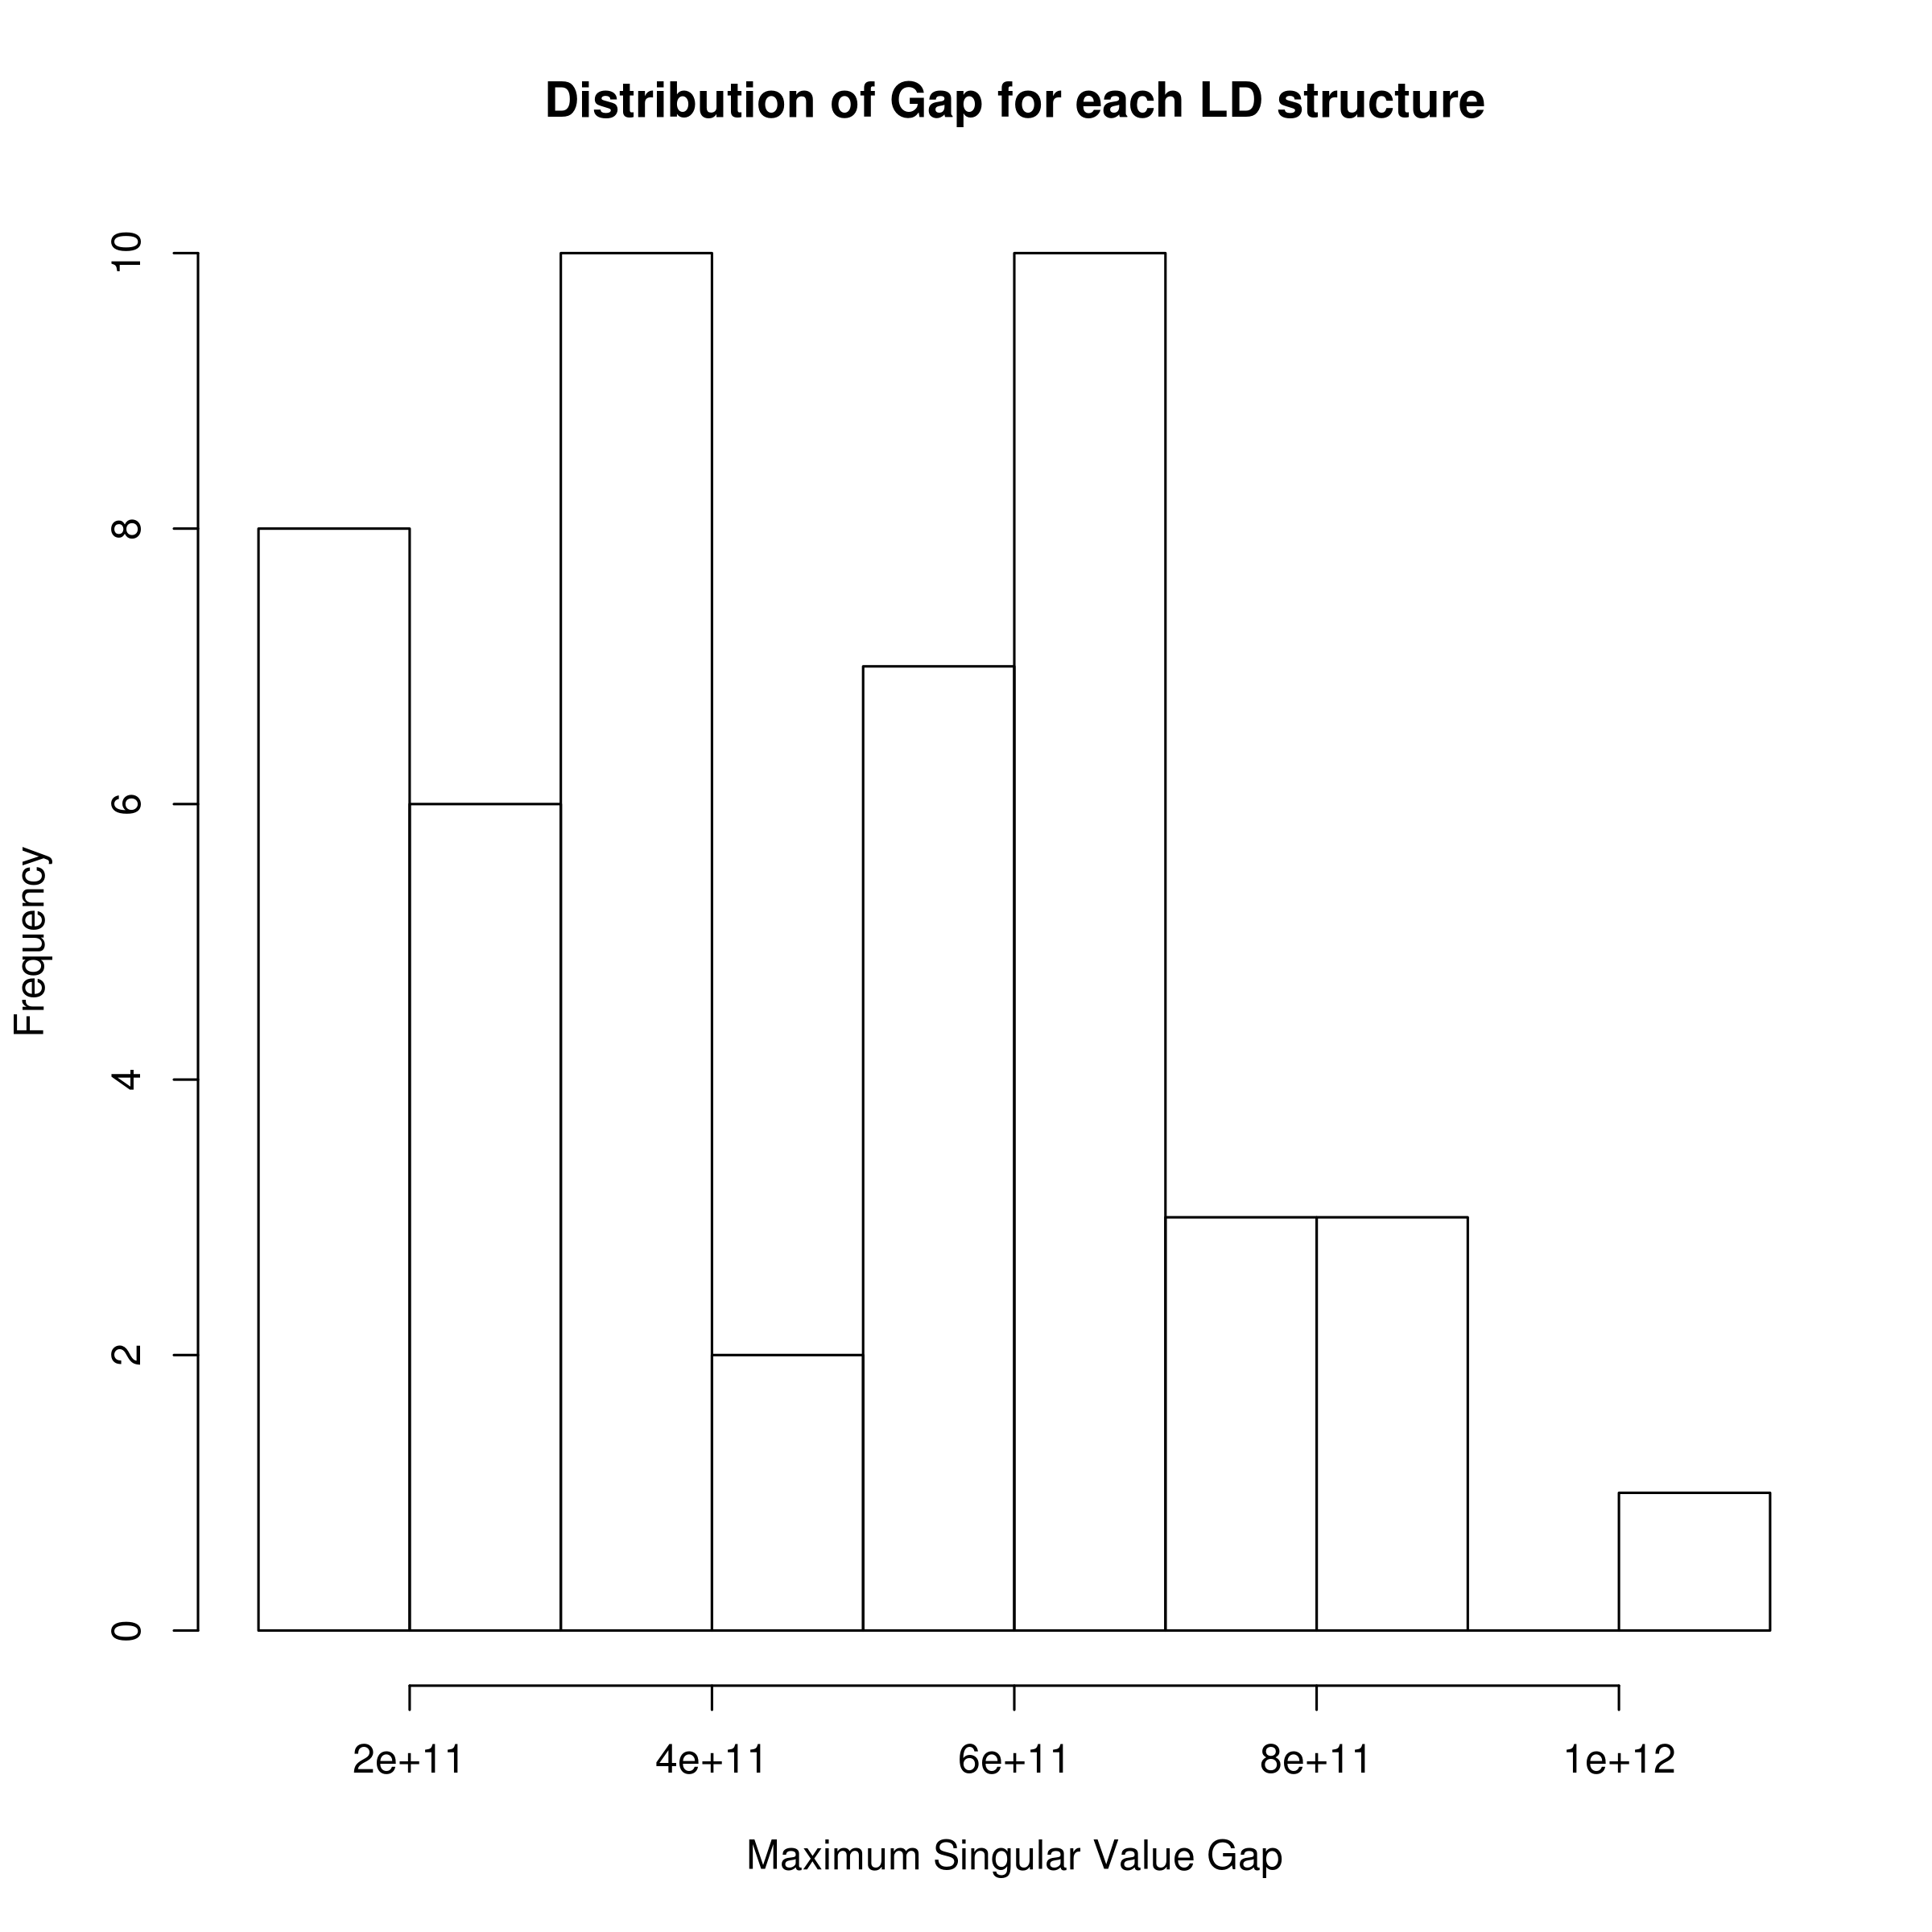
\includegraphics[width=0.5\textwidth]{figure/singular_value_distribution.png}
				\label{fig:singularValueDist}
				\vspace{-20pt}
			\end{figure}
			%\end{wrapfigure}
			
			By employing the \gls{tSVD} as a method for regularization, we were able to solve the ill-posed \cref{eq:shrekEq}, and obtain the estimated heritability.
						
		\subsection{Comparing with \glsentrylong{ldsc}}
			% main difference 
			Conceptually, the fundamental hypothesis of \gls{ldsc} and our algorithm were quite different.
			\gls{ldsc} were based on the ``global'' inflation of test statistic and its relationship to the \gls{LD} pattern.
			\gls{ldsc} hypothesize that the larger the \gls{LD} score, the more likely will the \gls{SNP} be able to ``tag'' the causal \gls{SNP} and the heritability can then be estimated through the regression between the \gls{LD} score and the test statistic.
			
			On the other hand, our algorithm focuses more on the per-\gls{SNP} level.
			Our main idea was that the individual test statistic of each \glspl{SNP} is a combination of its own effect and effect from \glspl{SNP} in \gls{LD} with it. 
			Thus, based on this concept, our algorithm aimed to ``remove'' the inflation of test statistic introduced through the \gls{LD} between \glspl{SNP} and the heritability can be calculated by adding the test statistic of all \glspl{SNP} after ``removing'' the inflation. 
			
			Mathematically, the calculation of \gls{ldsc} and our algorithm were also very different. 
			\gls{ldsc} take the sum of all $R^2$ within a 1cM region as the LD score and regress it against the test statistic to obtain the slope and intercept which represent the heritability and amount of confounding factors respectively. 
			In their model, \gls{ldsc} assume that each \glspl{SNP} will explain the same portion of heritability
			\begin{align}
			 \mathrm{Var}(\beta)&=\frac{h^2}{M}\boldsymbol{I}\\
			 M &= \text{number of SNPs}\notag\\
			 \beta &= \text{vector containing per normalized genotype effect sizes}\notag\\
			 I &= \text{identity matrix}\notag\\
			 h^2 &= \text{heritability}\notag
			\end{align}
			
			As for our algorithm, the whole \gls{LD} matrix were used and inverted to decompose the \gls{LD} from the test statistic. 
			There were no assumption of the amount of heritability explained by each \glspl{SNP}. 
			However, our algorithm does assumed that the null should be 1 and therefore cannot detect the amount of confounding factors. 
					
	\section{Assessing the Performance of Our Algorithm}
	\label{sec:shrekSim}
		First, we would like to test how well our algorithm works for heritability estimation under different scenarios.
		To account for different genetic architecture, we varies the heritability of the trait, the number of causal \glspl{SNP} and the genotypes(therefore varies the \gls{LD} pattern) during the quantitative trait simulation.
		
		\subsection{Sample Size}
		One important consideration in our simulation was the number of sample simulated. 
		The sample size was the most important parameter in determining the standard error of the heritability estimation. 
		As sample size increases, study will be more representative of the true population. 
		The increased number of information also means a better estimation of parameters, therefore a smaller \acrfull{se}.
		% awk -F "\t" '{print $2"\t"$9}' full | uniq | sed -e 's/[^0-9[:space:]]//g' | awk '{for(i=2;i<=NF;++i)j+=$i; print $1" "j; j=0}' | sort | uniq  %script for text mining
		Based on information from \gls{GWAS} catalog\citep{Welter2014}, we calculate the sample size distribution using simple text mining and exclude studies with conflicting sample size information in multiple entries. 
		The average sample size for all \gls{GWAS} recorded on the \gls{GWAS} catalog was 7,874, with a median count of 2,506 and a lower quartile at 940 (\cref{fig:gwasCata}). 
		We argue that if the algorithm works for studies with a small sample size (e.g lower quartile sample size), then it should perform even better when the sample size is larger. 
		Thus, we only simulate 1,000 samples in our simulation, which roughly represent the lower quartile sample size range.
		
		\begin{wrapfigure}{R}{8cm}
			\centering
			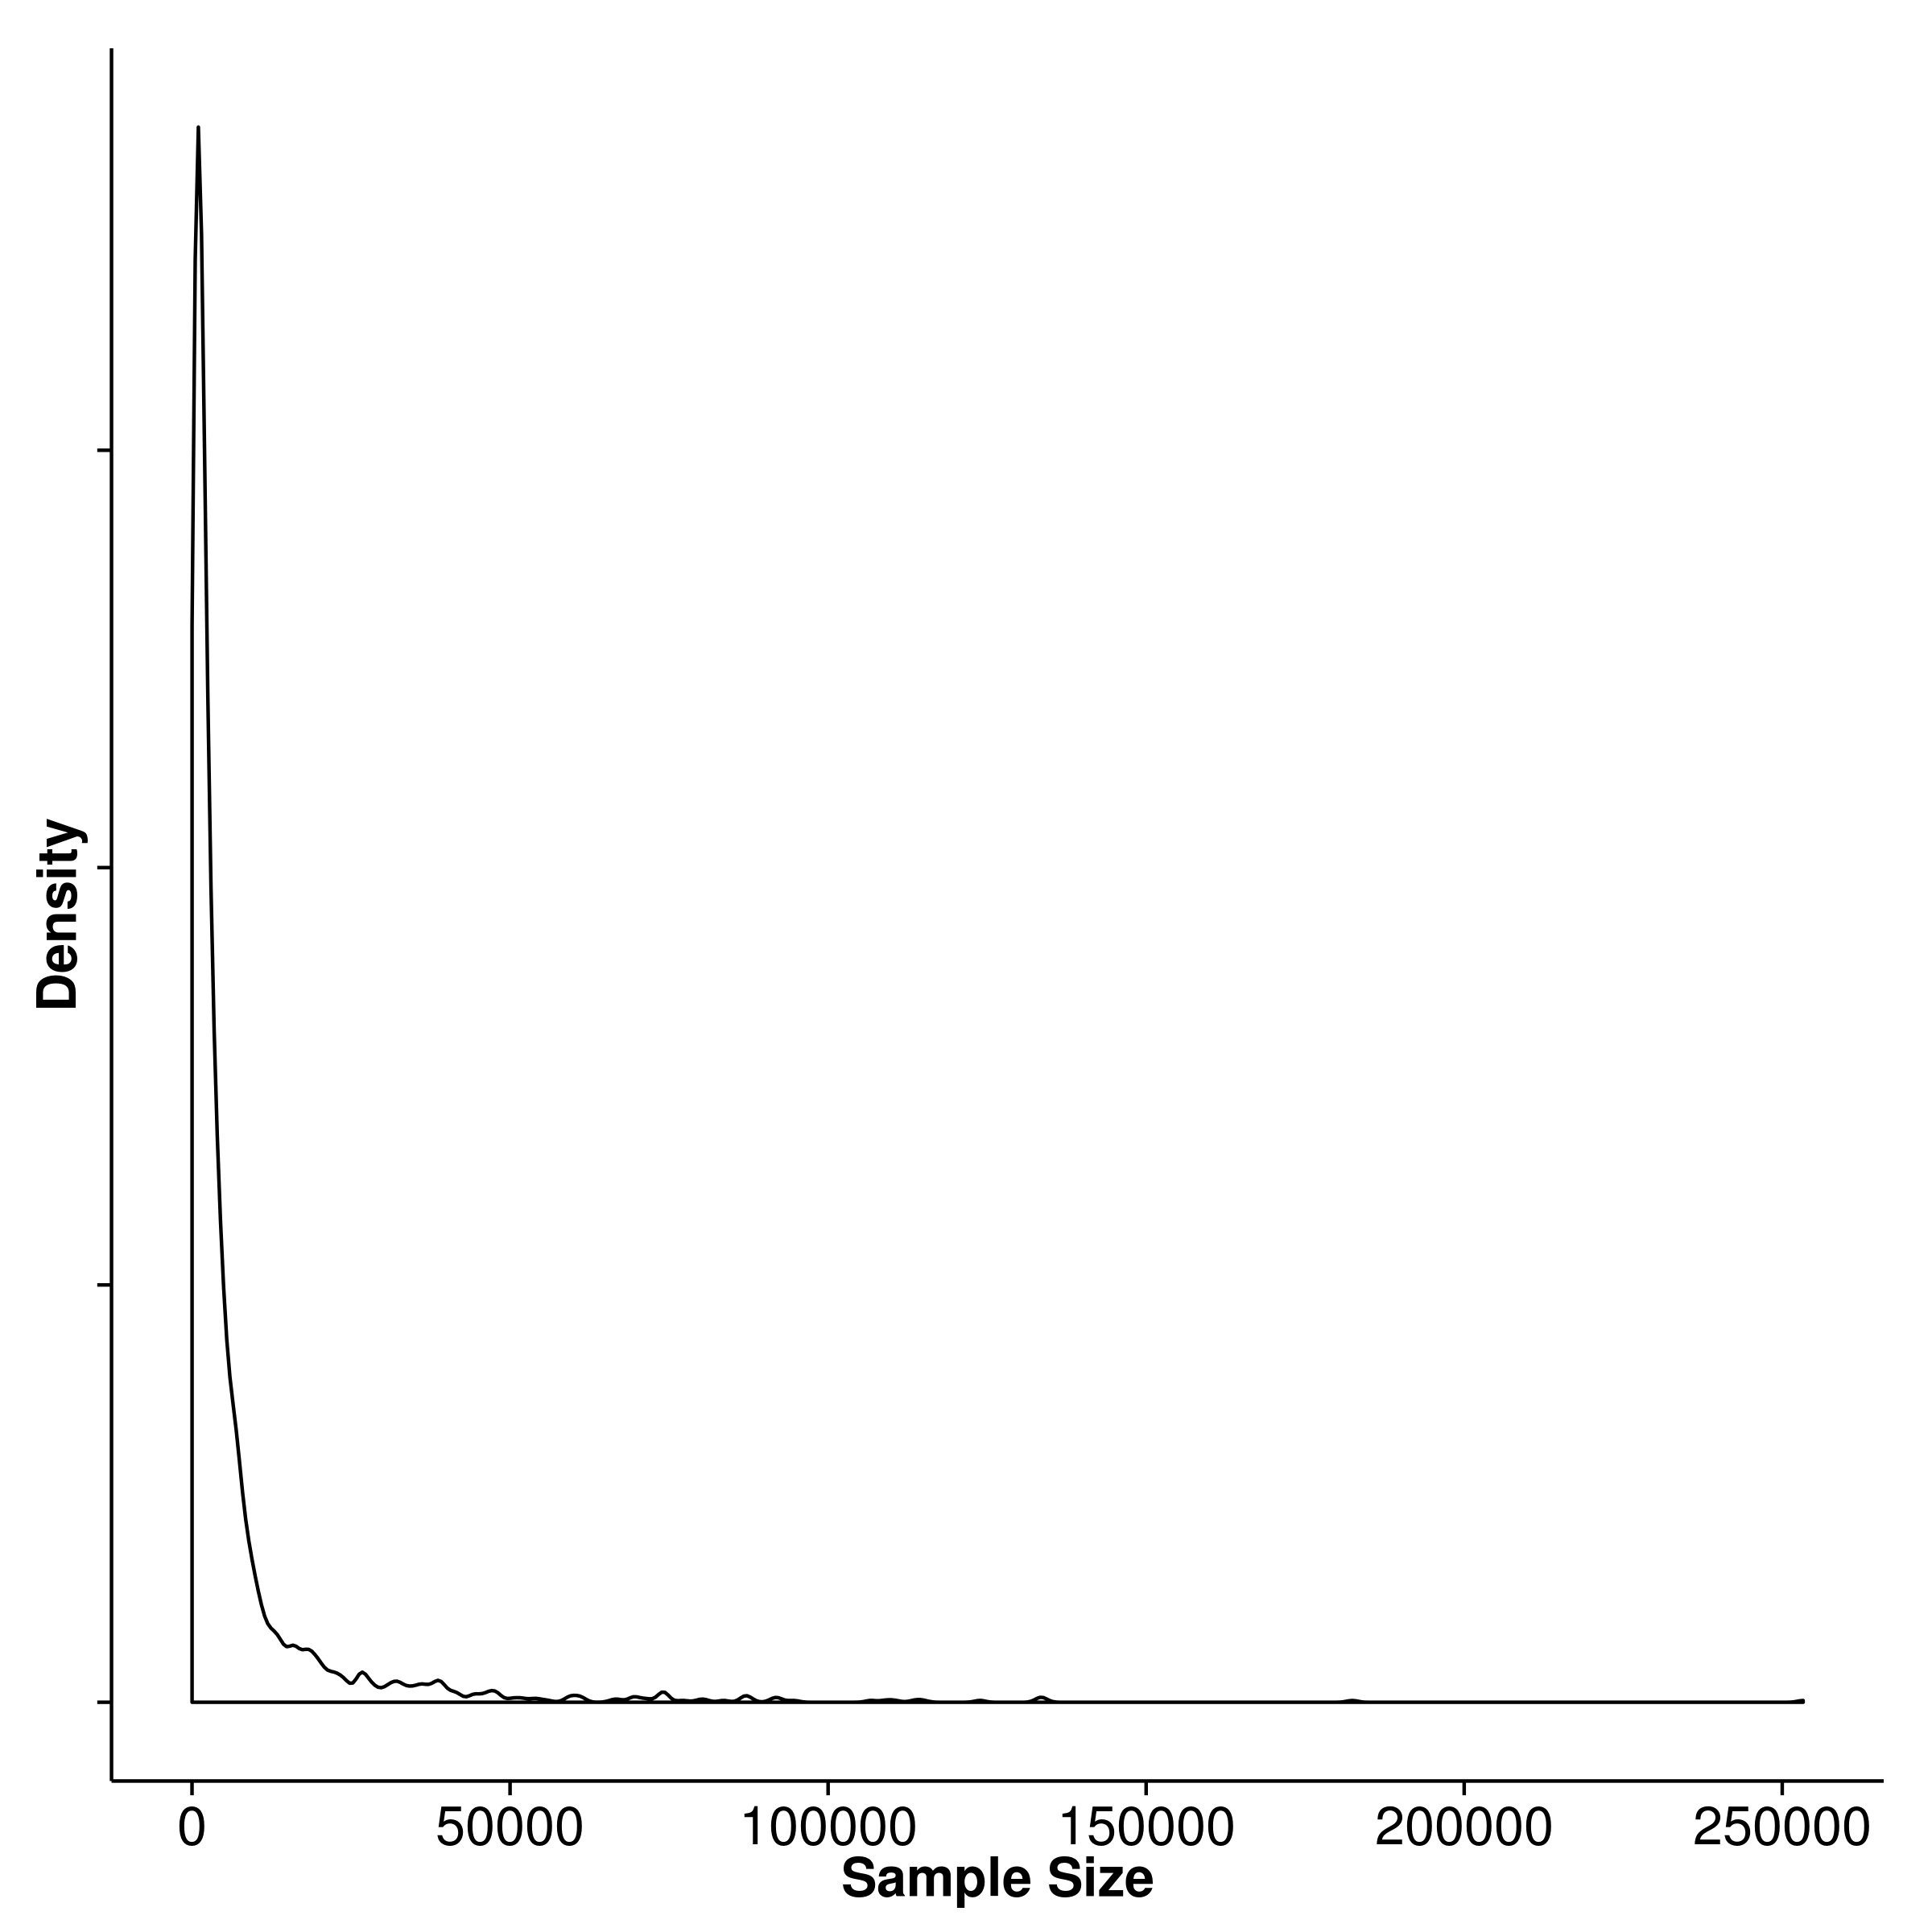
\includegraphics[width=0.5\textwidth]{figure/gwasSampleSize.png}
			\caption[GWAS Sample Size distribution]{
				\gls{GWAS} sample size distribution.
				}
			\label{fig:gwasCata}
		\end{wrapfigure}
		
		\subsection{Number of SNPs in Simulation}
		Another consideration in the simulation was the number of \glspl{SNP} included.
		In a typical \gls{GWAS} study, there are usually a larger number of \glspl{SNP} when compared to the sample size. 
		Fr example, in the \gls{pgc} \glng{scz} \gls{GWAS}, more than 9 million \glspl{SNP} were included, with around 700,000 \glspl{SNP} on chromosome 1.
		Although it would be idea to simulate 700,000 \glspl{SNP} in our simulation, the time required for simulating the samples will become unrealistic.
		
		As the number of \glspl{SNP} simulated grow, more time were required for the simulation of samples and more calculation will be required.
		Moreover, the increasing number of \glspl{SNP} will lead to increased size of the \gls{LD} matrix, requiring a long time for the inverse of the matrix.
		In reality, this should not be a real problem as one typically only calculate the heritability of the data set once and the speed of the algorithm is still relatively fast. 
		However, in the case of simulation where we would like to repeat the same analysis many times, the small increment of time will lead to an escalation in total simulation time, making the simulation infeasible. 
		To compromise, we simulate a total of 50,000 \glspl{SNP} from chromosome 1 as a balance between run time of simulation and the total \glspl{SNP} simulated.
		
		\subsection{Genetic Architecture}
		Of all simulation parameter, the genetic architecture was the most complicated and important parameter. 
		The \gls{LD} pattern, the number of causal \glspl{SNP}, the effect size of the causal \glspl{SNP} and the heritability of the trait were all important factors contribute to the genetic architecture of a trait. 
		
		First and foremost, because the aim of the algorithm was to estimating the heritability of the trait, it is important that the algorithm works for traits from different heritability spectrum.
		We therefore simulate traits with heritability ranging from 0 to 0.9, with increment of 0.1.
		
		Secondly, in real life scenario, the ``causal'' variant might not be readily included on the \gls{GWAS} chip and were only ``tagged'' by \glspl{SNP} included on the \gls{GWAS} chip.
		However, to simplify our simulation, all ``causal'' variants were included in our simulation (e.g. perfectly ``tagged'')
		
		Thirdly, to obtain a realistic \gls{LD} pattern, we simulate the genotypes using the HAPGEN2 programme\citep{Su2011}, using the 1000 genome \gls{CEU} haplotypes as an input.
		In short, HAPGEN2 simulate new haplotypes as an imperfect mosaic of haplotpyes from a reference panel and the haplotypes that have already been simulated using the \textit{Li and Stephens} (LS) model of \gls{LD} \citep{Li2003}.
		In a typical \gls{GWAS} , one usually only have power in detecting ``common variants'', usually defined as variants with \gls{maf} $\ge 0.01$.
		We therefore only consider scenario with ``common'' variants and only use \glspl{SNP} with \gls{maf} $\ge0.1$ in the \gls{CEU} haplotypes as an input to HAPGEN2. 
		This will reduce the probability of having \glspl{SNP} with \gls{maf} $<0.01$ in the final simulated sample sets.
		
		Finally, we would like to simulate traits with different inheritance model such as oligogenic traits and polygenic traits.
		We therefore varies the number of causal \glspl{SNP} ($k$) with $k\in\{5, 10, 50, 100, 250, 500\}$.
		An important consideration in the simulation of causal \glspl{SNP} is the effect size distribution. 
		\citet{Orr1998} suggested that the exponential distribution can be used to approximate the genetic architecture of adaptation. 
		As a result of that, we used the exponential distribution with $\lambda=1$ as an approximation to the effect size distribution:
		\begin{align}
		\theta&=\mathrm{exp}(\lambda=1)\notag\\
		\beta&=\pm\sqrt{\frac{\theta \times h^2}{\sum \theta}}
		\label{eq:randomEffect}
		\end{align}
		with a random direction of effect.
		
		Given the normalized genotype as $\boldsymbol{X}$ and the simulated heritability as $h^2$, the phenotype can then be calculated as 
		\begin{align}
		\epsilon_i&\sim N(0,\sqrt{\mathrm{Var}(\boldsymbol{X\beta})\frac{1-h^2}{h^2}} )\notag\\
		\boldsymbol{\epsilon} &= (\epsilon_1,\epsilon_2,...,\epsilon_n)^t\notag\\
		\boldsymbol{y} &= \boldsymbol{X\beta}+\boldsymbol{\epsilon}
		\label{eq:simulationOfPhenotype}
		\end{align}
		
		The test statistics were then calculated using the plink programme \citep{Purcell2007} and input to our algorithm to estimate the heritability. 
		An independent 500 samples were simulated as a reference panel for the calculation of \gls{LD} matrix as in reality, we should not have the sample genotype for the construction of the \gls{LD} matrix. 
		The whole process will be repeated 50 times such that a distribution of the estimate can be obtained. 
		The whole simulation process can be viewed as follow:
		We simulate a large population of samples (e.g. $50\times1,000+500 = 50,500$) where 500 samples were randomly selected as a reference panel. 
		In the subsequent iteration of simulation, 1,000 samples were randomly selected from the population \textit{without replacement} and estimation were performed.
		We then simulate 10 different population and repeat the whole process.
		
		In summary:
		\begin{enumerate}
			\item Randomly select 50,000 \glspl{SNP} with \gls{maf}$>0.1$ from chromosome 1
			\item Simulate 500 samples using HAPGEN2 and used as a reference panel
			\item Randomly generate $k$ effect size with $k \in \{5,10,50,100,250,500\}$ following  \cref{eq:randomEffect}
			\item Randomly assign the effect size to $k$ \glspl{SNP}
			\item Simulate 1,000 samples using HAPGEN2 and calculate their phenotype according to \cref{eq:simulationOfPhenotype}
			\item Perform heritability estimation using our algorithm
			\item Repeat step 5-6 50 times
			\item Repeat step 1-7 10 times
		\end{enumerate}
		
		\section{Comparison with Other Programmes}
		It is also important for us to compare our algorithm to existing methods for the performance in estimating the narrow sense heritability.
		We would also like to extend the simulation to other conditions such as quantitative traits with extreme effect size distribution, case control studies and quantitative traits with extreme phenotype selections.
		
		Currently, the only other programme that is capable to estimate the narrow sense heritability using only test statistic is the \gls{ldsc} \citep{Bulik-Sullivan2015}. 
		On the other hand, \gls{gcta} \citep{Yang2011} is commonly considered as the golden standard for heritability estimation in \gls{GWAS} data. 
		Therefore, we choose to compare the performance of our algorithm to that of \gls{ldsc} and \gls{gcta}.
		It is important to note that as we are assessing the performance of the programme through controlled simulation, there should be little confounding factors. 
		For \gls{ldsc}, the default intercept estimation function allows it to estimate and correct for confounding factors with an increase in \gls{se}. 
		The simulation will therefore be unfair to \gls{ldsc} with intercept estimation, as the \gls{se} is increased yet there are little confounding factors for it to correct.
		Thus, we also simulate \gls{ldsc} with a fixed intercept (-{}-no-intercept) parameters to avoid bias against \gls{ldsc}.	
		
		\subsection{Simulation}
		We first repeated the whole simulation process in \cref{sec:shrekSim} by including \gls{gcta}, \gls{ldsc} with fixed intercept and \gls{ldsc} with intercept estimation on top of our algorithm. 
		The sample genotype was provided to \gls{gcta} for the calculation of the genetic relationship matrix and the estimation of heritability.
		On the other hand, the \gls{LD} score for \gls{ldsc} were calculated using the same simulated reference panel as our algorithm to simulate conditions where the sample genotype was not available.
		So the simulation follows the following procedure:
		
		\begin{enumerate}
			\item Randomly select 50,000 \glspl{SNP} with \gls{maf}$>0.1$ from chromosome 1
			\item Simulate 500 samples using HAPGEN2 and used as a reference panel
			\item Randomly generate $k$ effect size with $k \in \{5,10,50,100,250,500\}$ following  \cref{eq:randomEffect}
			\item Randomly assign the effect size to $k$ \glspl{SNP}
			\item Simulate 1,000 samples using HAPGEN2 and calculate their phenotype according to \cref{eq:simulationOfPhenotype}
			\item Perform heritability estimation using our algorithm, \gls{gcta}, \gls{ldsc} with fixed intercept and \gls{ldsc} with intercept estimation.
			\item Repeat step 5-6 50 times
			\item Repeat step 1-7 10 times
		\end{enumerate}
		
		\subsection{Extreme Effect Size}
		On top of the original quantitative trait simulation, another condition we were interested in was the performance of the algorithms when there is a small amount of \glspl{SNP} with a much larger effect size.
		This can be observed in disease such as %HERE
		
		To simulate extreme effect size, we consider scenarios where $m$ \glspl{SNP} accounts 50\% of all the effect size with $m\in\{1,5,10\}$.
		The effect size was then calculated as
		\begin{align}
		\beta_{eL} &= \pm\sqrt{\frac{0.5h^2}{m}} \notag\\
		\beta_{eS} &= \pm\sqrt{\frac{0.5h^2}{100-m}} \notag\\
		\beta &= \{\beta_{eL}, \beta_{eS}\}
		\label{eq:extremEffect}
		\end{align}
		The effect size were then randomly assigned to 100 causal \glspl{SNP} and phenotype will be calculated as in \cref{eq:simulationOfPhenotype}.
		The simulation procedure then becomes
		\begin{enumerate}
			\item Randomly select 50,000 \glspl{SNP} with \gls{maf}$>0.1$ from chromosome 1
			\item Simulate 500 samples using HAPGEN2 and used as a reference panel
			\item Randomly generate 100 effect size where $m$ has extreme effect, following \cref{eq:extremEffect}, with $m\in\{1,5,10\}$
			\item Randomly assign the effect size to 100 \glspl{SNP}
			\item Simulate 1,000 samples using HAPGEN2 and calculate their phenotype according to \cref{eq:simulationOfPhenotype}
			\item Perform heritability estimation using our algorithm, \gls{ldsc} with fixed intercept, \gls{ldsc} with intercept estimation and \gls{gcta}
			\item Repeat step 5-6 50 times
			\item Repeat step 1-7 10 times
		\end{enumerate}
		
		\subsection{Case Control Studies}
		The simulation of case control studies was similar to the simulation of quantitative trait. 
		However, there were two additional parameters to consider: the population prevalence and the observed prevalence.
		These parameters were required to simulate the samples under a liability model for case control studies.

		Although there were only two additional parameter, it is significantly more challenging for to simulate when compared to the simulation of quantitative traits.
		It is mainly because of the number of samples required to simulate adequate samples under the liability threshold model.
		Take for example, if one like to simulate a trait with population prevalence of $p$ and observed prevalence of $q$ and would like to have $n$ cases in total, one will have to simulate $\min(\frac{n}{p}, \frac{n}{q})$ samples.
		Considering the scenario where the observed prevalence is 50\%, the population prevalence is 1\%, if we want to simulate 1,000 cases, a minimum of 100,000 samples will be required.
		
		Given limited computer resources, it will be infeasible for us to simulate 1,000 cases with 50,000 \glspl{SNP} when the population prevalence is small.
		To simplify the simulation and reduce the burden of computation, we limited the observed prevalence to 50\% and varies the population prevalence $p$ such that $p\in\{0.5, 0.1, 0.05, 0.01\}$.
		Most importantly, we reduce the number of \glspl{SNP} simulated to 5,000 on chromosome 22 instead of 50,000 \glspl{SNP} on chromosome 1. 
		The change from chromosome 1 to chromosome 22 allow us to reduce the number of \glspl{SNP} without changing much of the \gls{SNP} density. 
		We acknowledged that the current simulation was relatively brief, however, it should serves as a prove of concept simulation to study the performance of the algorithms under the case control scenario.
		
		In the case control simulation, we randomly select 5,000 \glspl{SNP} from chromosome 22 with \gls{maf} $\ge0.1$ in the \gls{CEU} haplotypes as an input to HAPGEN2. 
		We then randomly select 100 \glspl{SNP} with effect size simulated based on \cref{eq:randomEffect}.
		In order to simulate a case control samples with 1,000 cases, we then simulate $\frac{1,000}{p}$ samples and calculate their phenotype using \cref{eq:simulationOfPhenotype}.
		The phenotype was then standardized and cases were defined as sample with phenotype passing the liability threshold with respect to $p$.
		An equal amount of samples were then randomly selected from samples with phenotype lower than the liability threshold and defined as controls.
			
		Finally, the case control simulation were performed as:
		\begin{enumerate}
			\item Randomly select 5,000 \glspl{SNP} with \gls{maf}$>0.1$ from chromosome 22
			\item Simulate 500 samples using HAPGEN2 and used as a reference panel
			\item Randomly generate 100 effect size following  \cref{eq:randomEffect}
			\item Randomly assign the effect size to 100 \glspl{SNP}
			\item Simulate $\frac{1,000}{p}$ samples using HAPGEN2 and calculate their phenotype according to \cref{eq:simulationOfPhenotype}
			\item Define case control status using the liability threshold and randomly select same number of case and controls for subsequent simulation
			\item Perform heritability estimation using our algorithm, \gls{ldsc} with fixed intercept, \gls{ldsc} with intercept estimation and \gls{gcta}
			\item Repeat step 5-7 50 times
			\item Repeat step 1-8 10 times
		\end{enumerate}
		
		\subsection{Extreme Phenotype Selection}
		The simulation of extreme phenotype selection was the same as the quantitative trait simulation. 
		The only difference being that instead of using all samples for heritability estimation, we only use the extreme 10\% of samples among the population for the heritability estimation.
		In brief, instead of simulating 1,000 samples, we simulate 5,000 samples following the exact procedure in the quantitative trait simulation with random effect size.
		However, after simulation of the phenotype using \cref{eq:simulationOfPhenotype}, we standardize the phenotype and only select the top 10\% and bottom 10\% samples (500 samples each) from the sample distribution.
		We then perform the same simulation procedure as in the quantitative trait simulation with random effect size.
		
		It was noted that the extreme phenotype selection were not supported by the \gls{ldsc} and \gls{gcta}.
		To allow comparison in such scenario, we apply the extreme phenotype adjustment from \citet{Sham2014} to the estimation obtained from \gls{ldsc} and \gls{gcta}.
		
	\section{Result}
		The heritabilibty estimation were implemented in \gls{shrek} and is available on \url{https://github.com/choishingwan/shrek}.  
		\subsection{Performance}
		
		To study the performance of \gls{shrek} and \gls{ldsc} in comparison to \gls{gcta}, we performed a variety of simulations to model scenarios with different number of causal \glspl{SNP}, different effect size distribution and different type of traits. 
		
		First, we examined the performance of the algorithms under the quantitative trait scenario. 
		In the quantitative trait scenario, we varies the number of causal \glspl{SNP} and either assigned an equal effect size to each causal \glspl{SNP} or assigned a per-allele effect sizes drawn from the squared root of the exponential distribution with $\lambda=1$.
		
		\subsection{Quantitative Trait Simulation with Equal Effect Size}
		% QT Equal Effect
		
		\begin{figure}
			\centering
			\subfloat[SHREK]{
				\scalebox{.4}{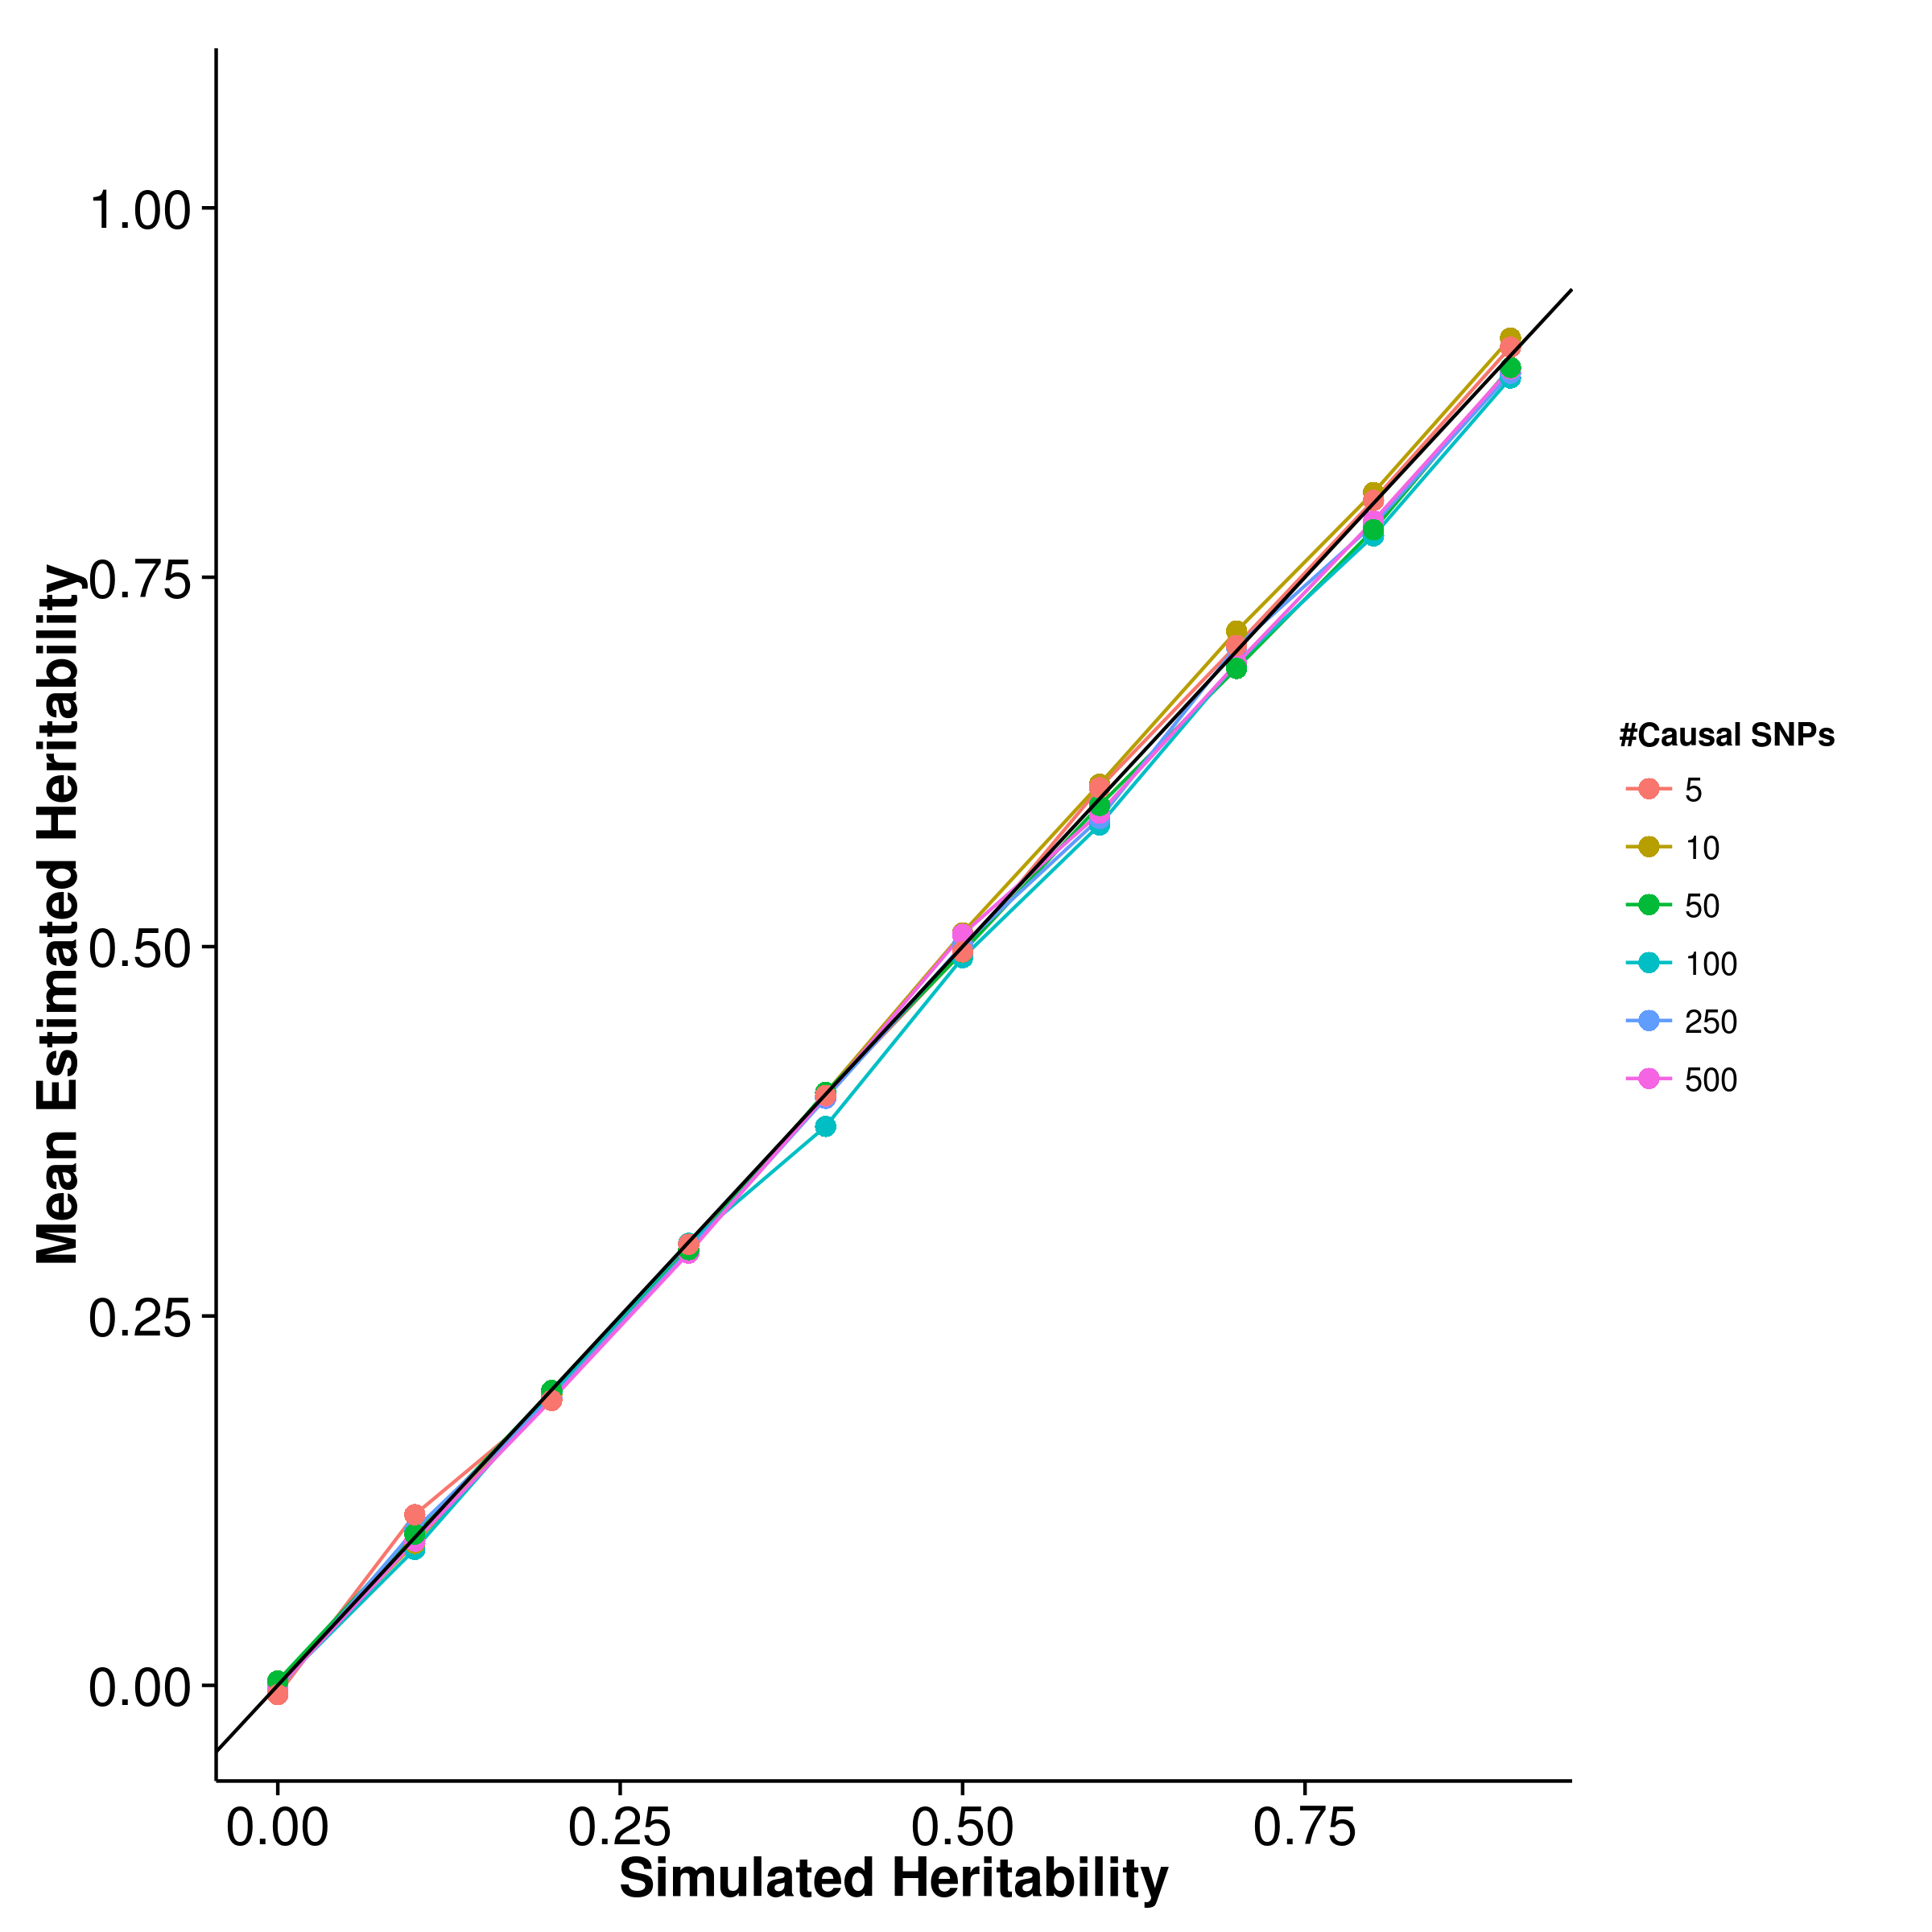
\includegraphics{figure/he_summary/equal/shrek_Qt_Equal_mean.png}}
				\label{fig:shrekQtEqualMean}
			}
			\subfloat[GCTA]{
				\scalebox{.4}{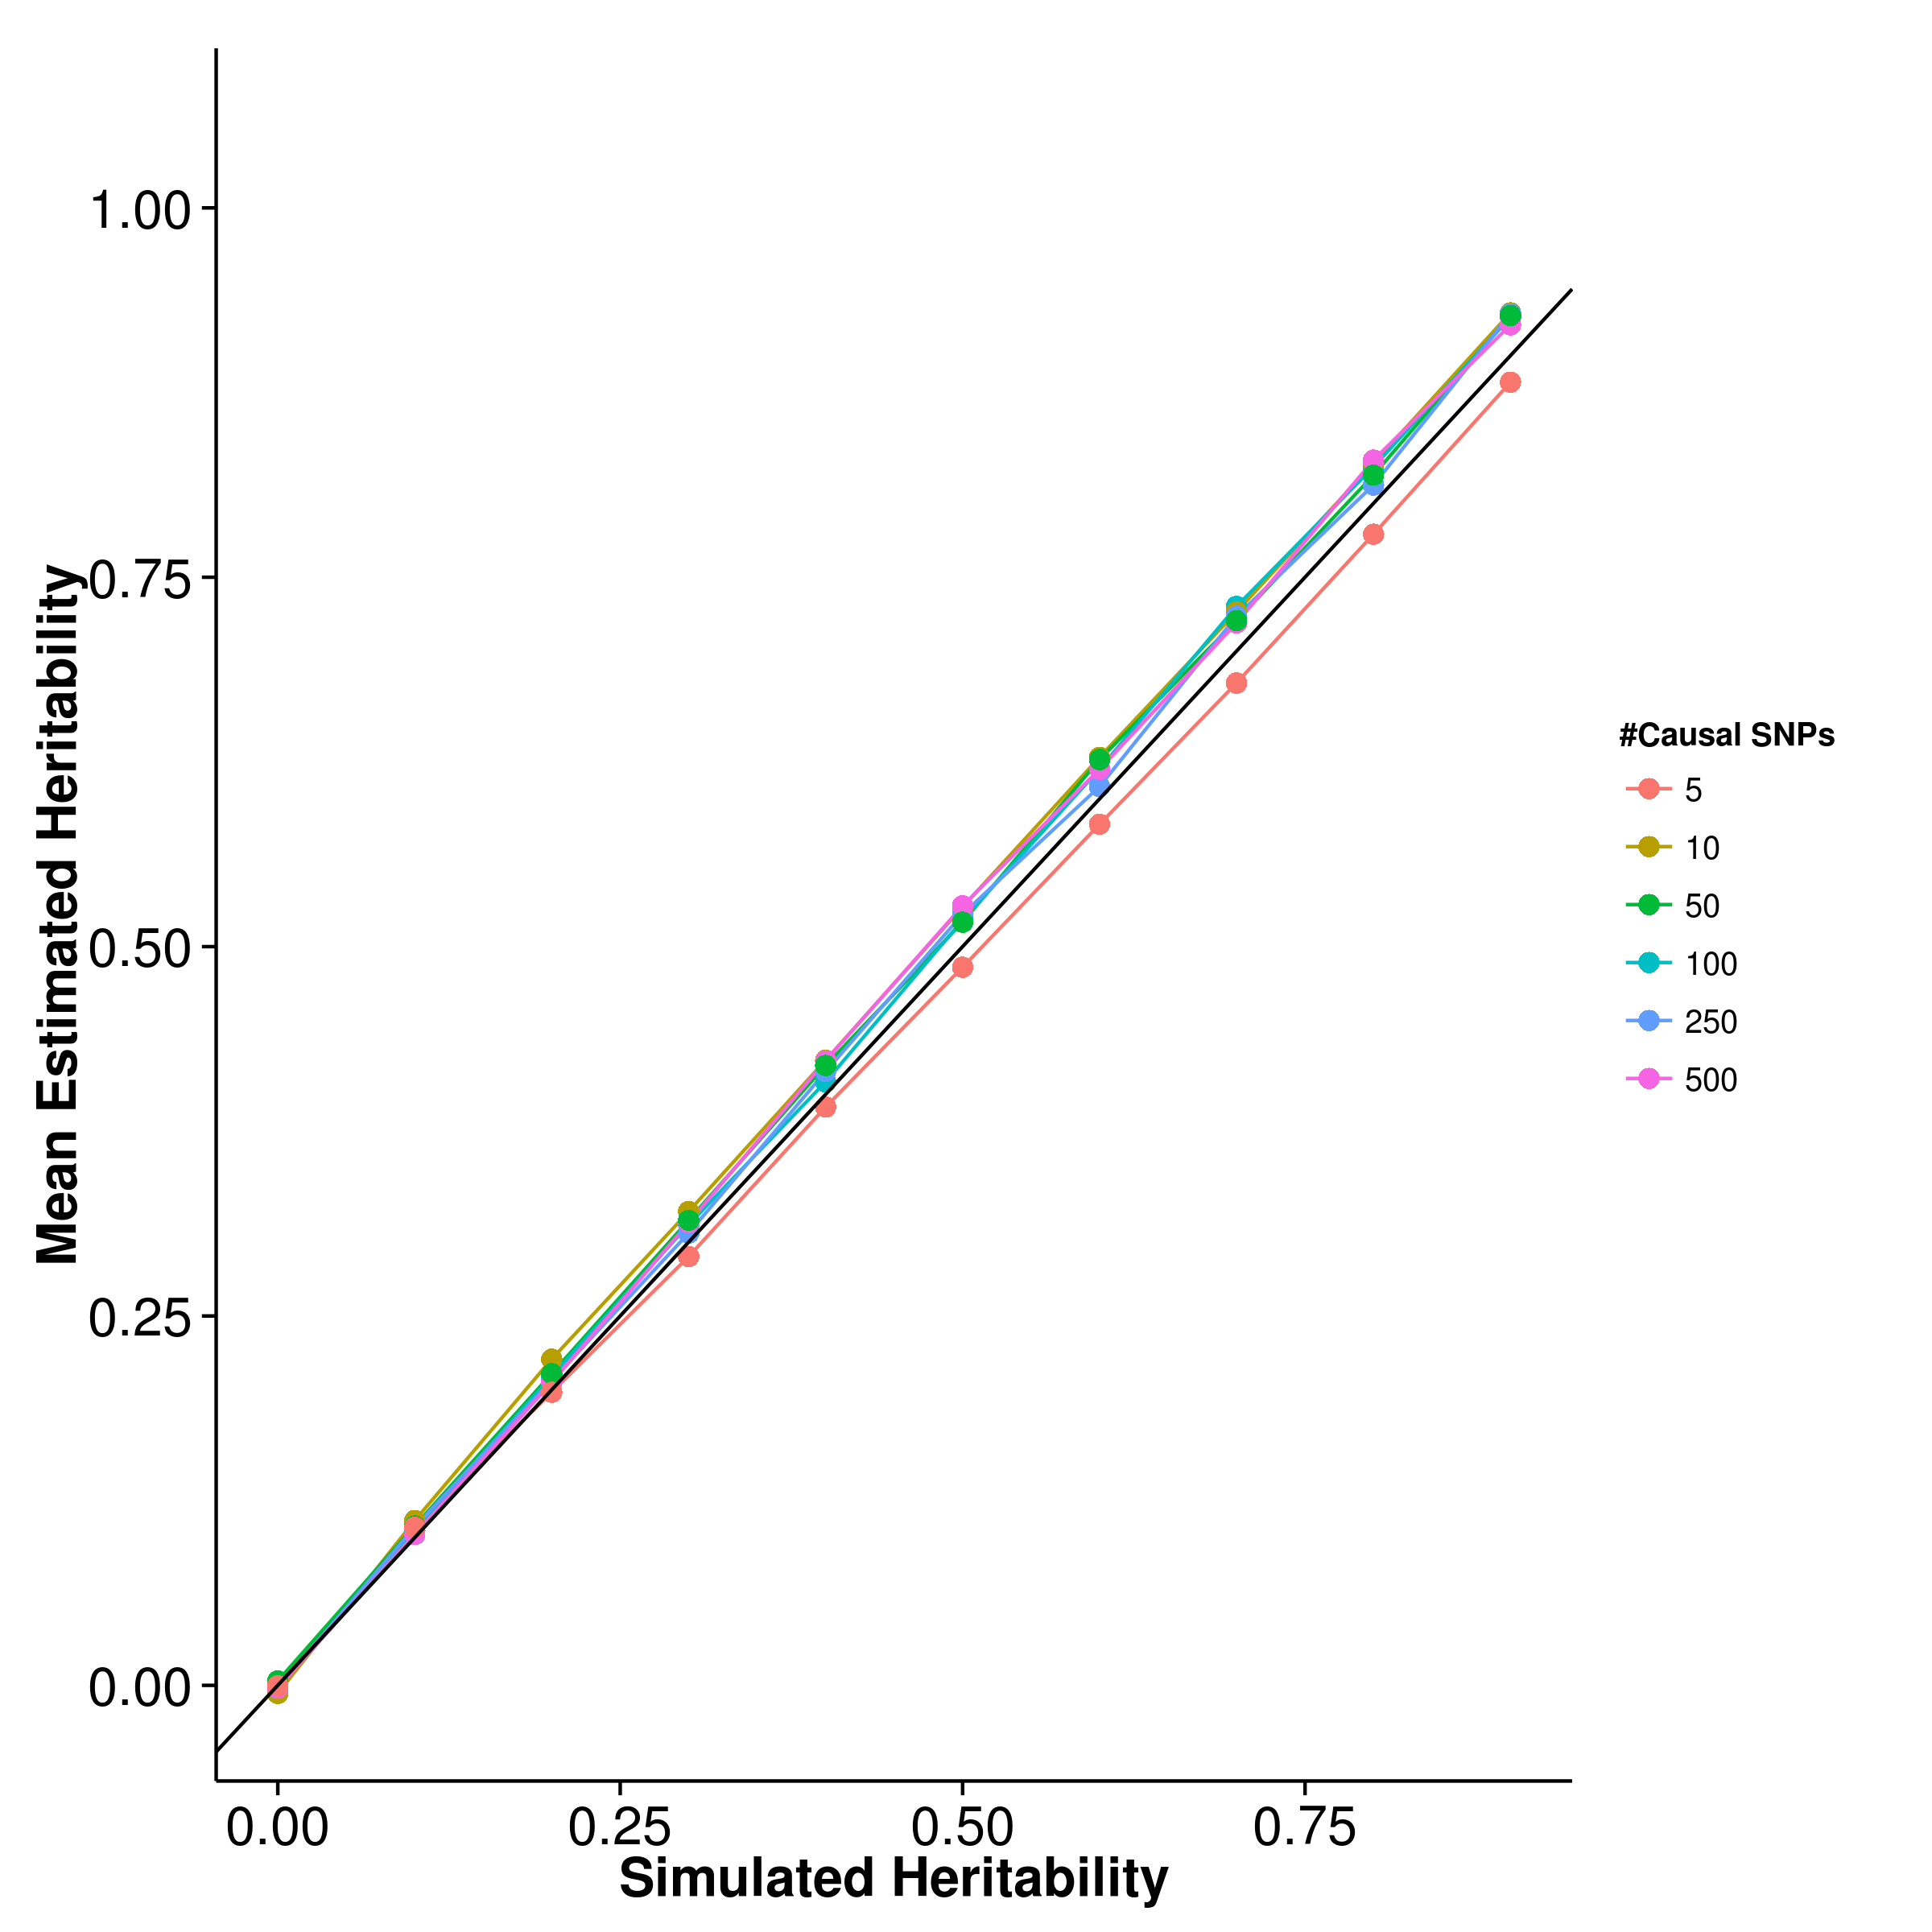
\includegraphics{figure/he_summary/equal/gcta_Qt_Equal_mean.png}}
				\label{fig:gctaQtEqualMean}
			}\\
			\subfloat[LDSC with fix intercept]{
				\scalebox{.4}{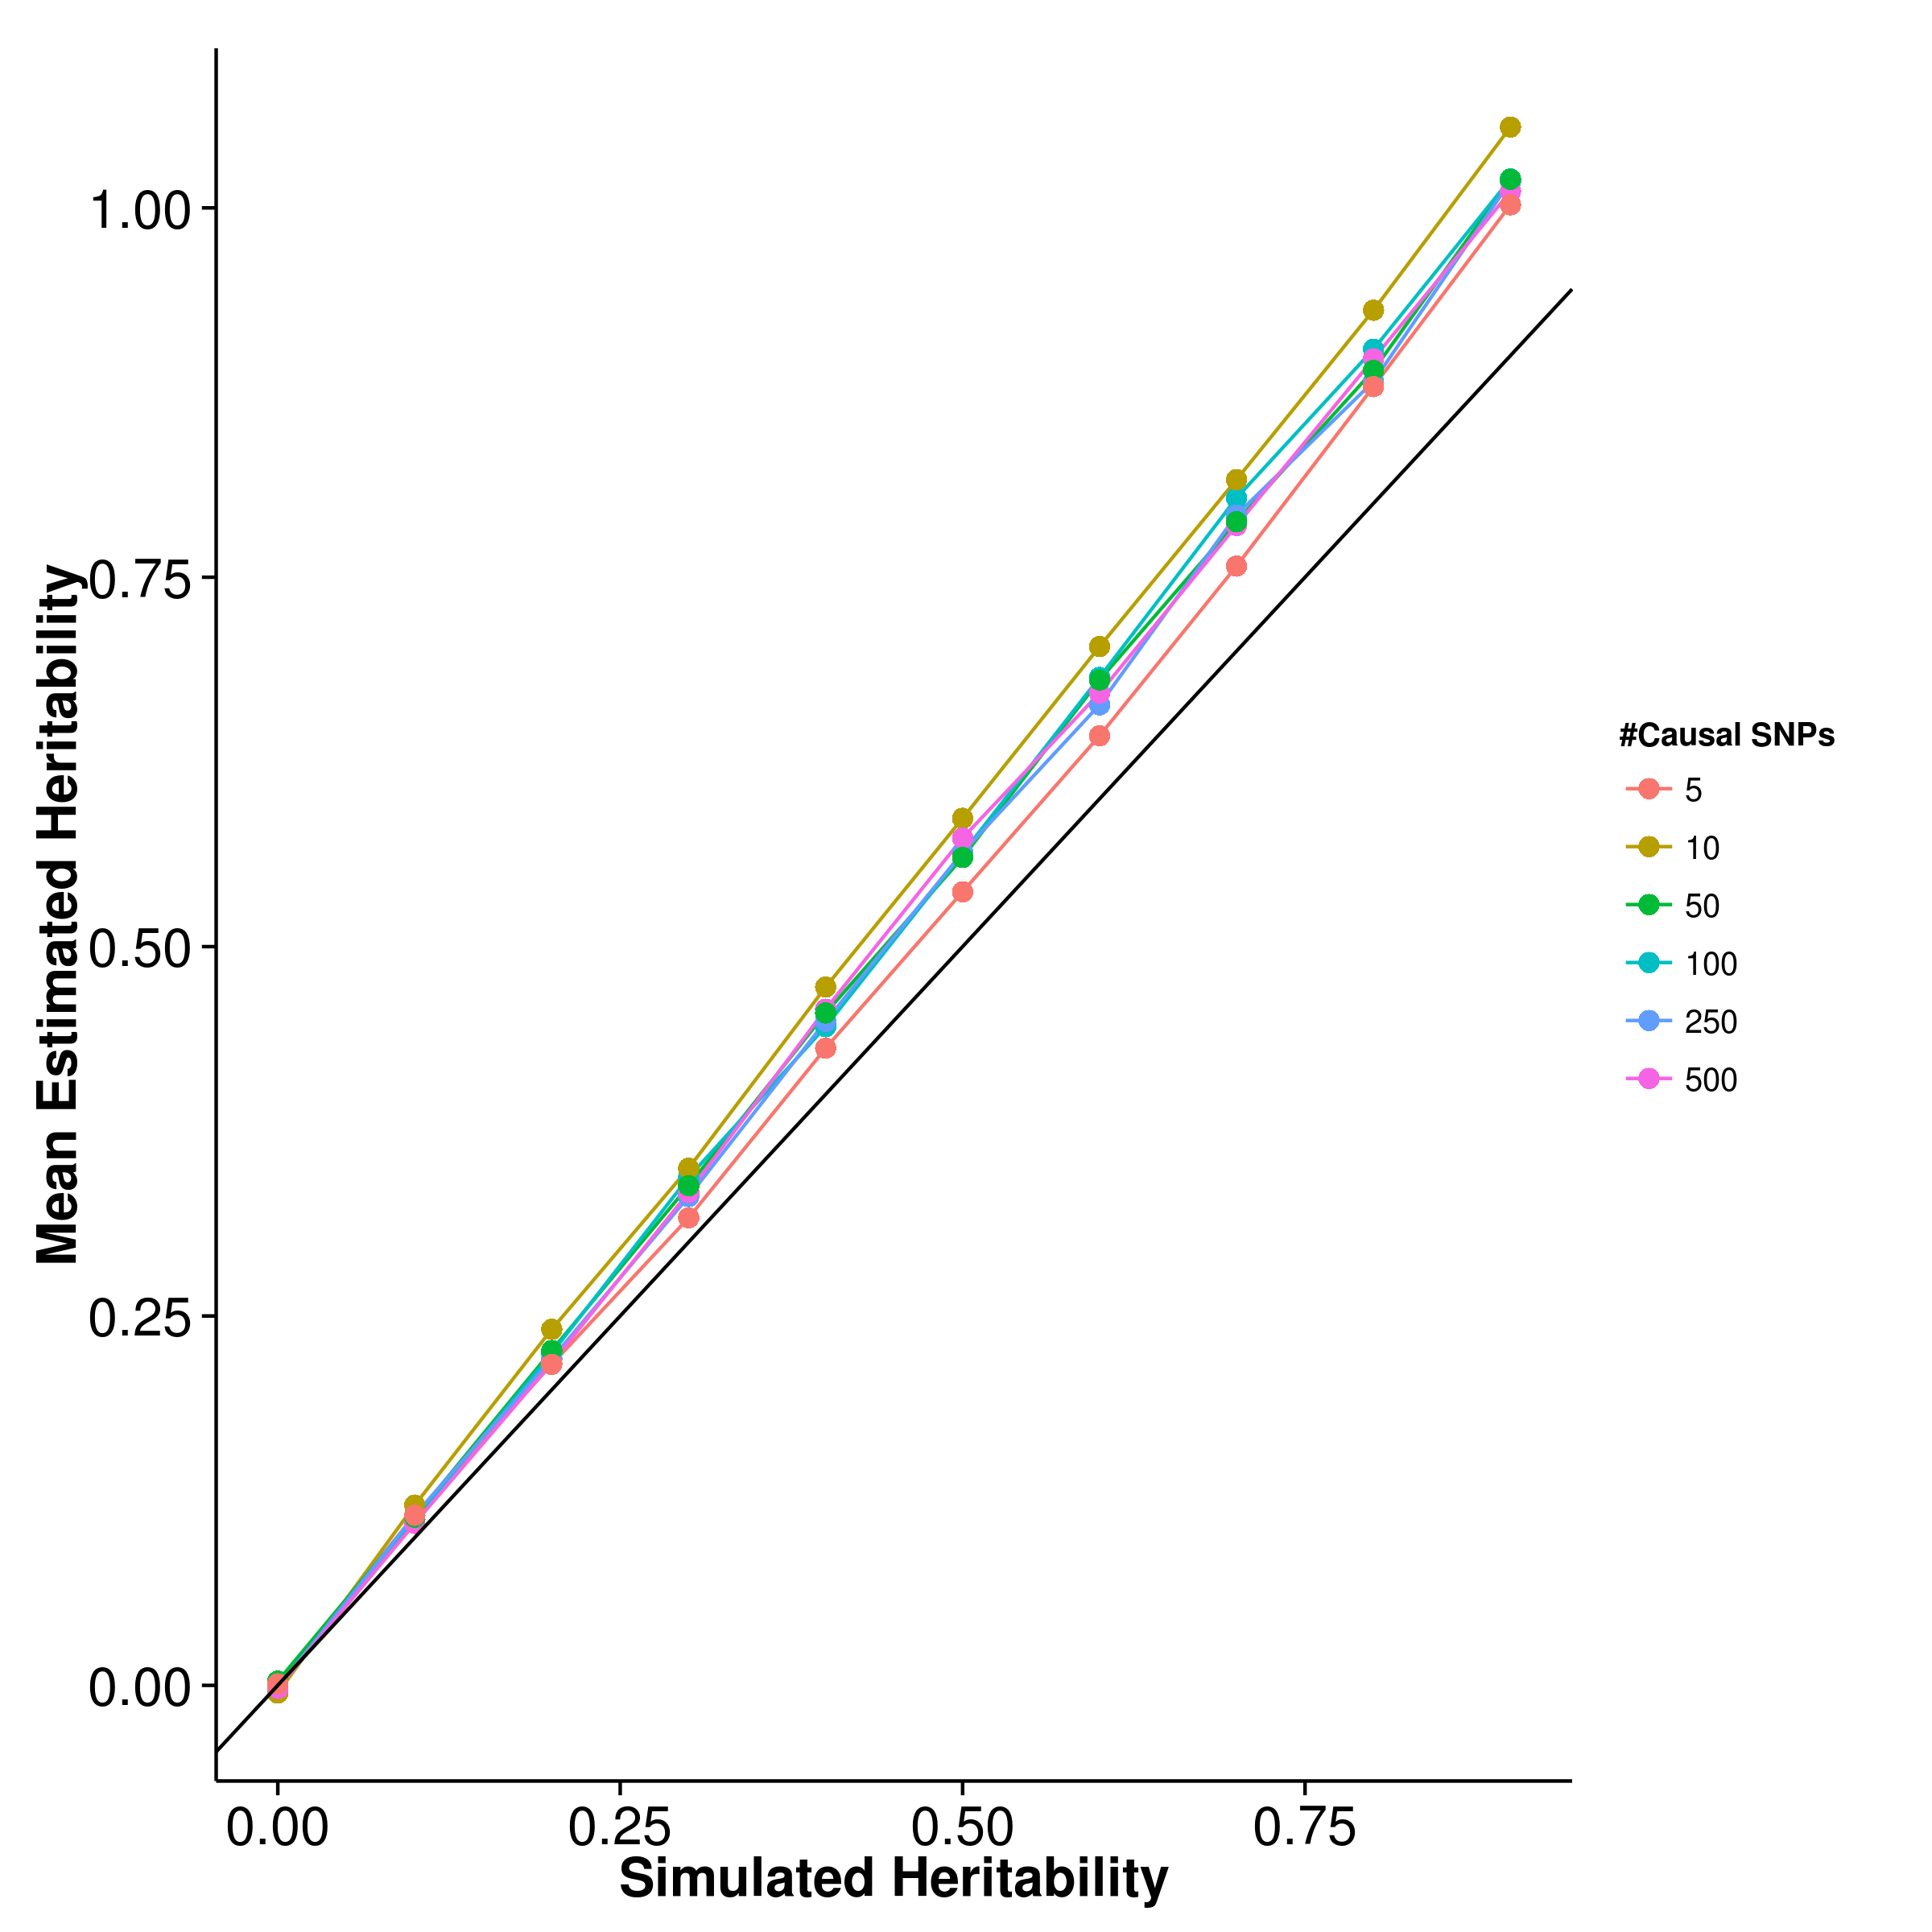
\includegraphics{figure/he_summary/equal/ldsc_Qt_Equal_mean.png}}
				\label{fig:ldscQtEqualMean}
			}
			\subfloat[LDSC with intercept estimation]{
				
				\scalebox{.4}{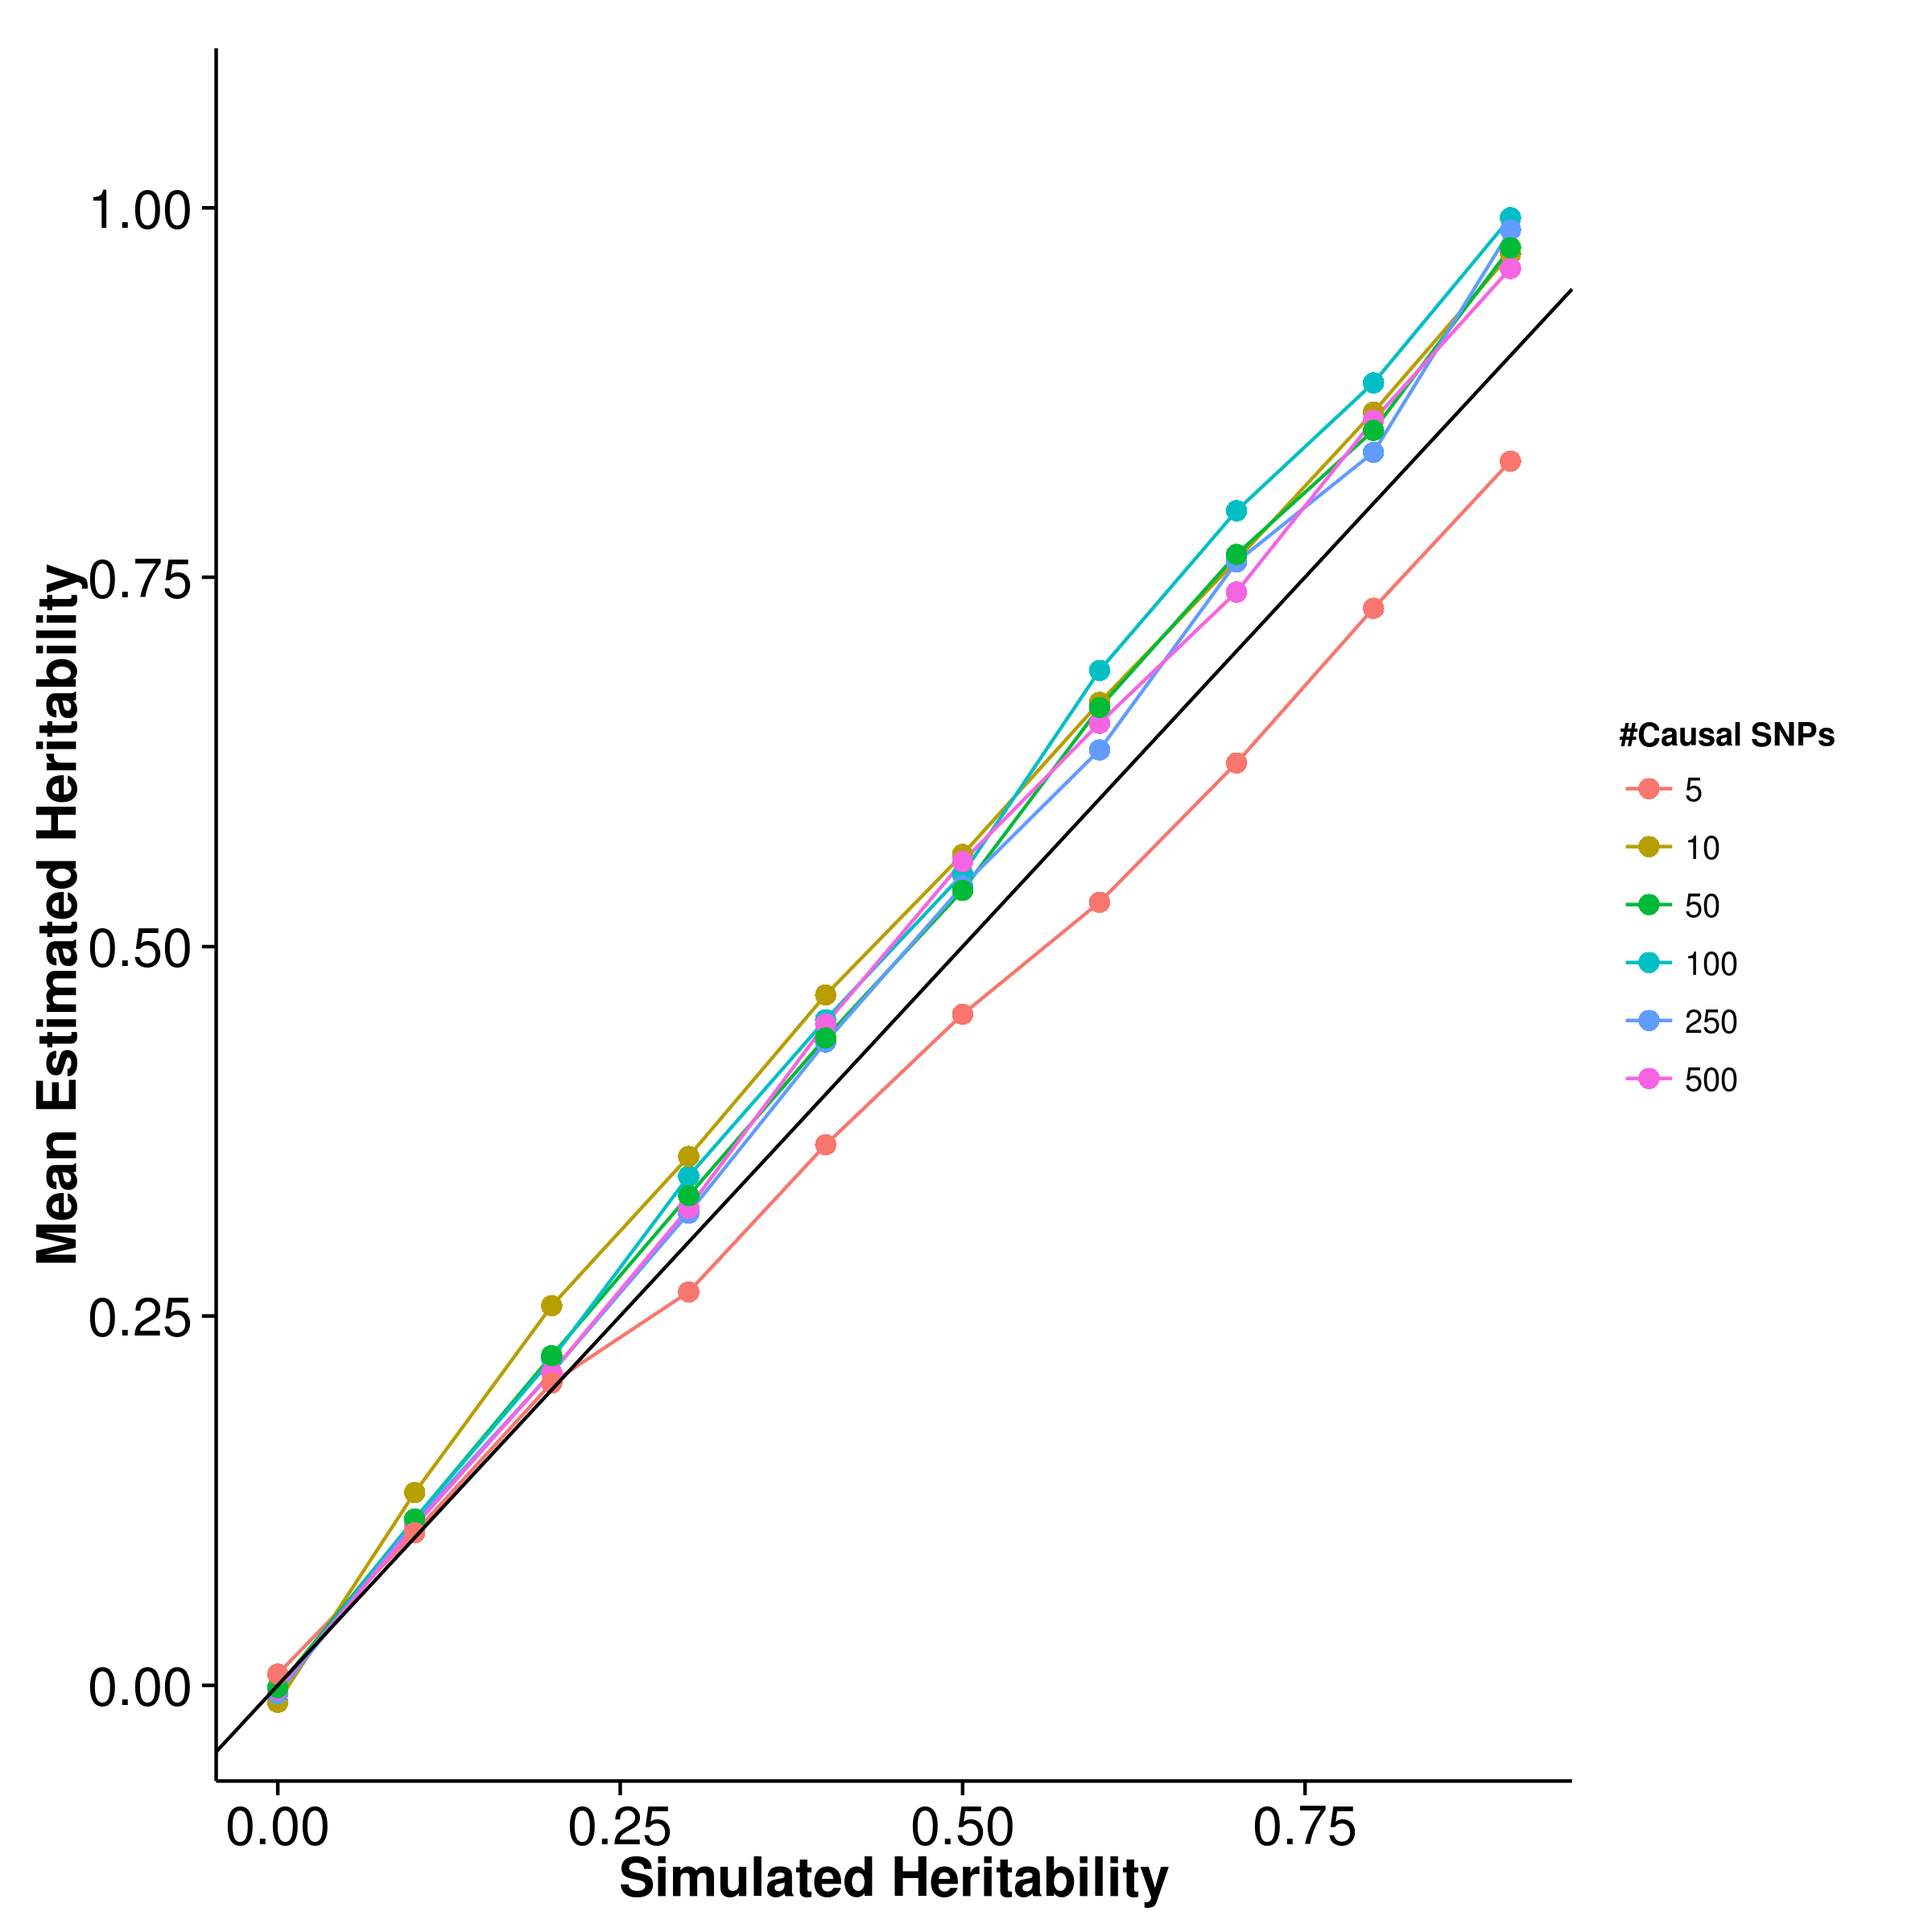
\includegraphics{figure/he_summary/equal/ldscIn_Qt_Equal_mean.png}}
				\label{fig:ldscInQtEqualMean}
			}
			\caption[Quantitative Trait with Equal Effect Size Simulation Result(Mean)]
			{Mean of results from quantitative trait simulation with equal effect size simulation.
				\gls{shrek} was found to be less biased of all the tools whereas there was a slight upward bias for \gls{ldsc} when the intercept was fixed, especially when the number of causal \glspl{SNP} was small.} 
			\label{fig:QtEqualMean}
		\end{figure}
		
		\begin{figure}
			\centering
			\subfloat[SHREK]{
				\scalebox{.4}{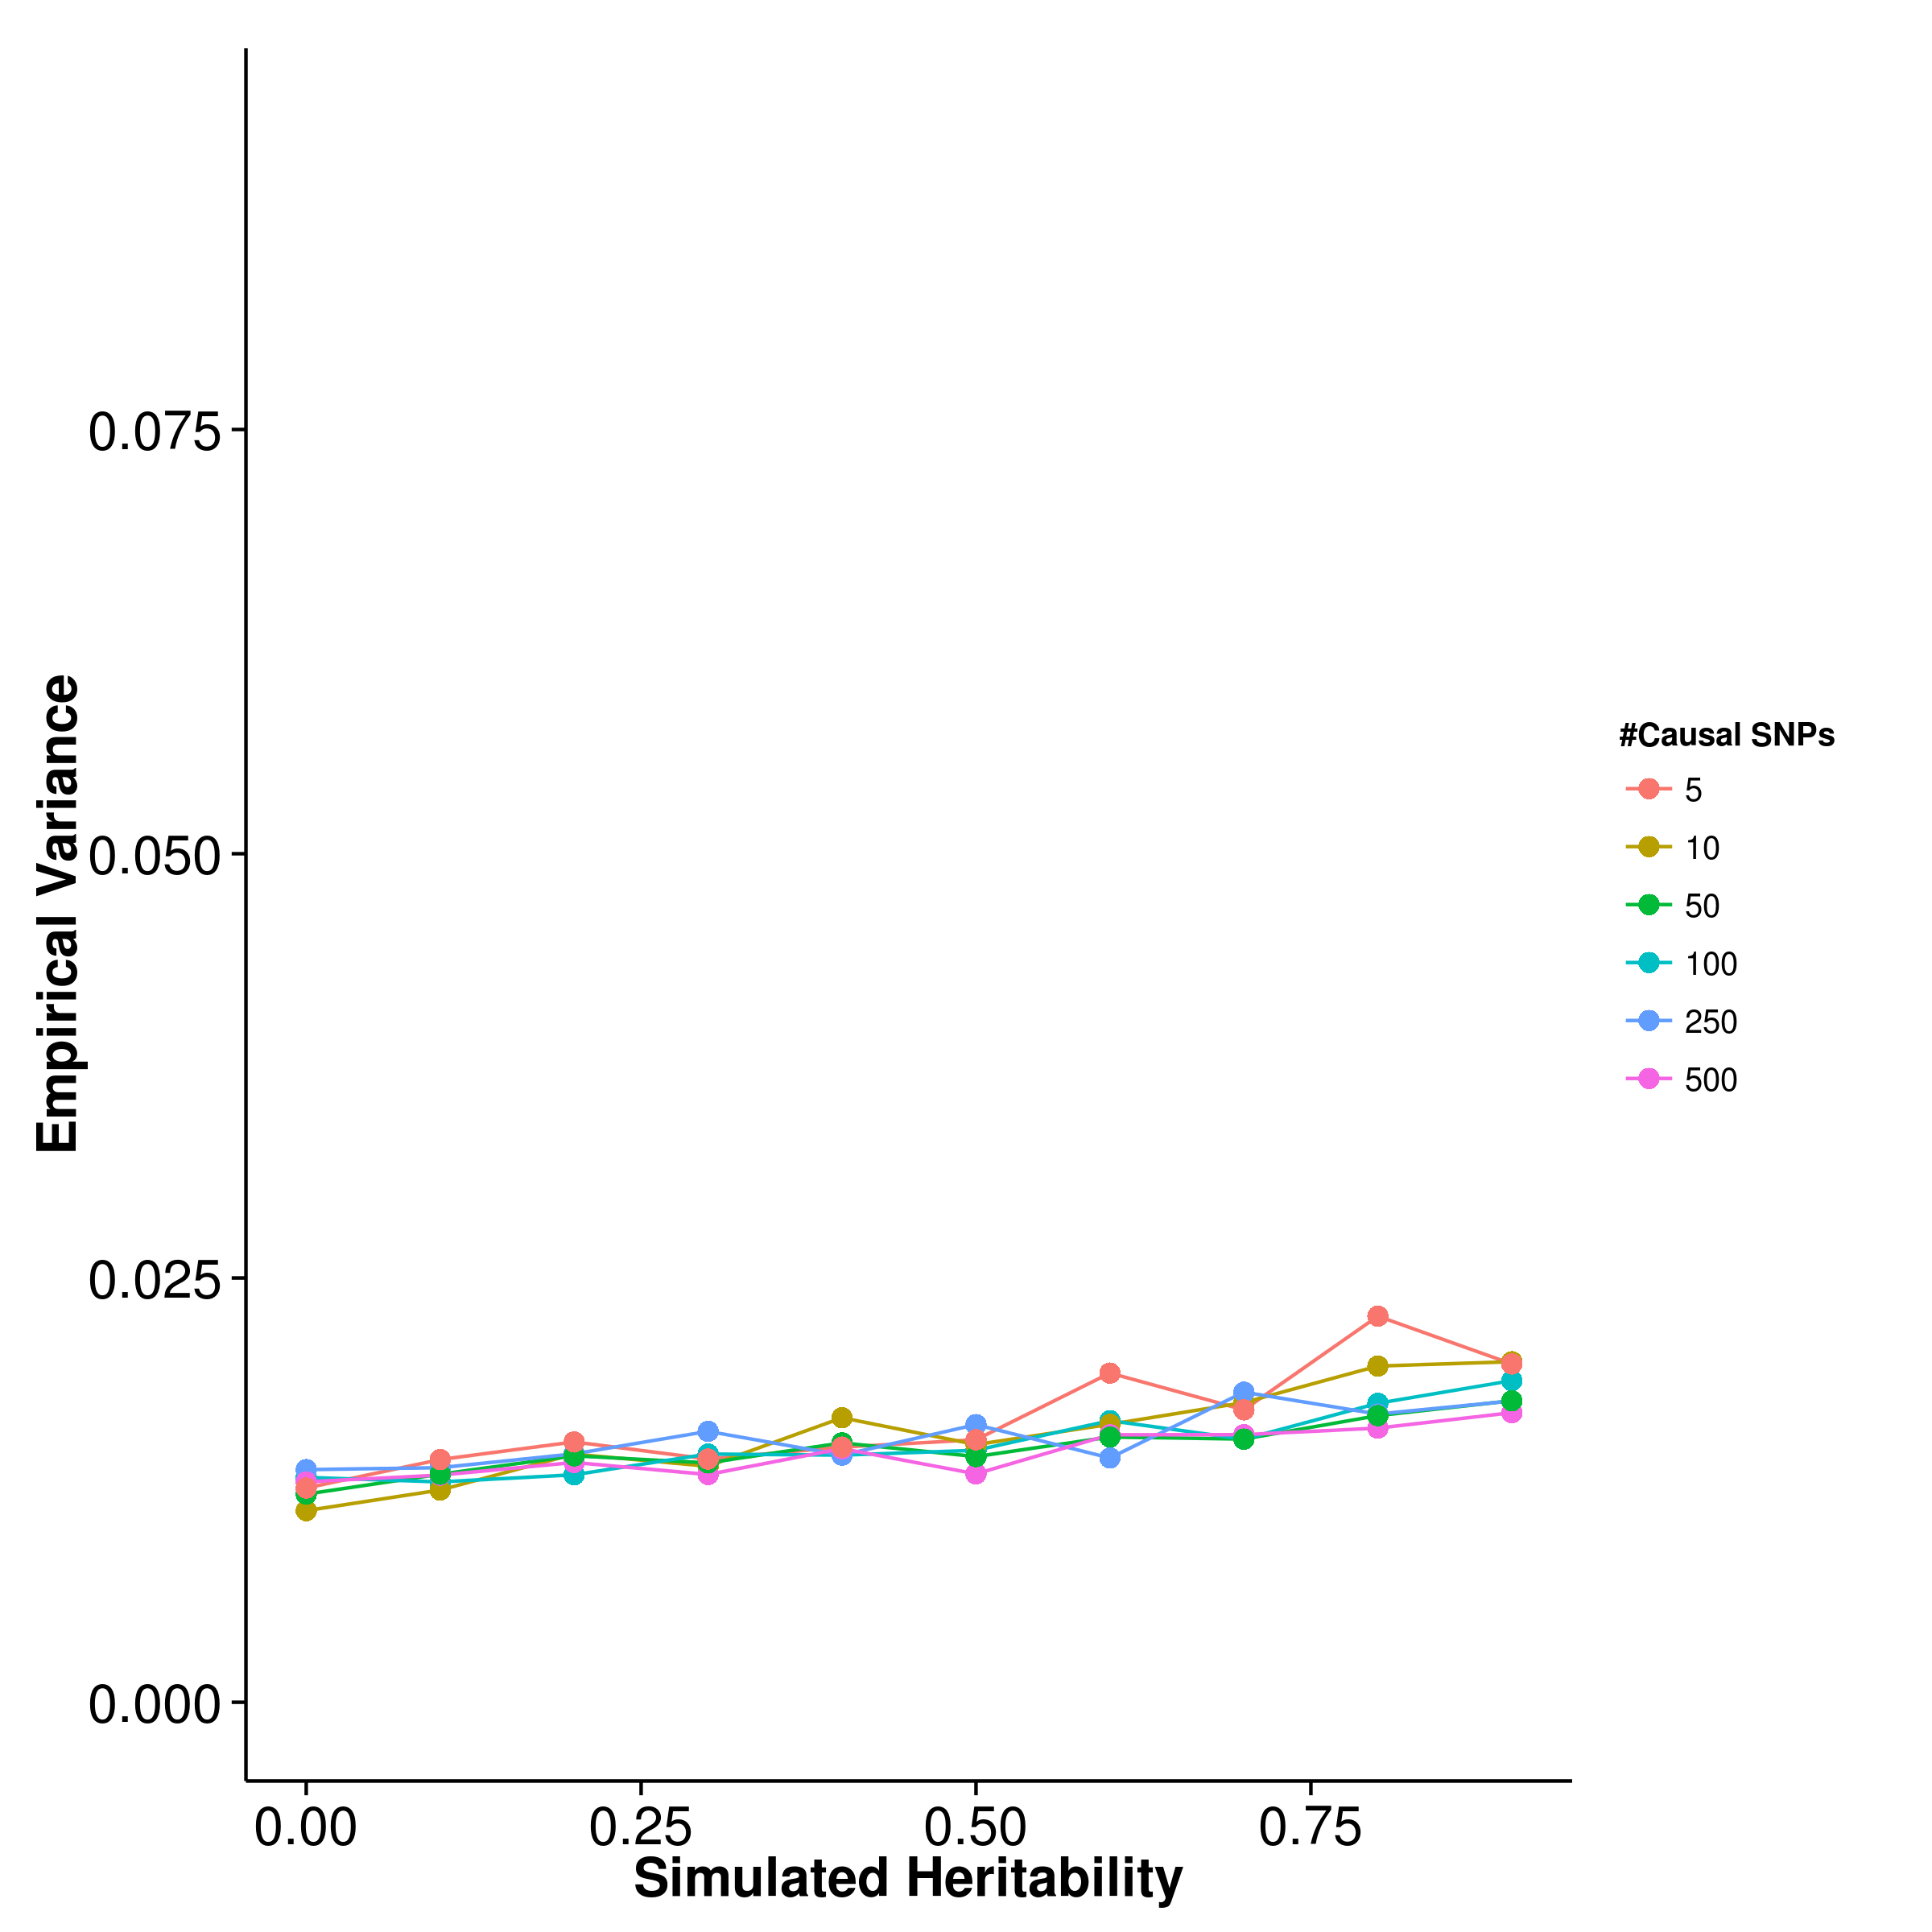
\includegraphics{figure/he_summary/equal/shrek_Qt_Equal_sd.png}}
				\label{fig:shrekQtEqualVar}
			}
			\subfloat[GCTA]{
				\scalebox{.4}{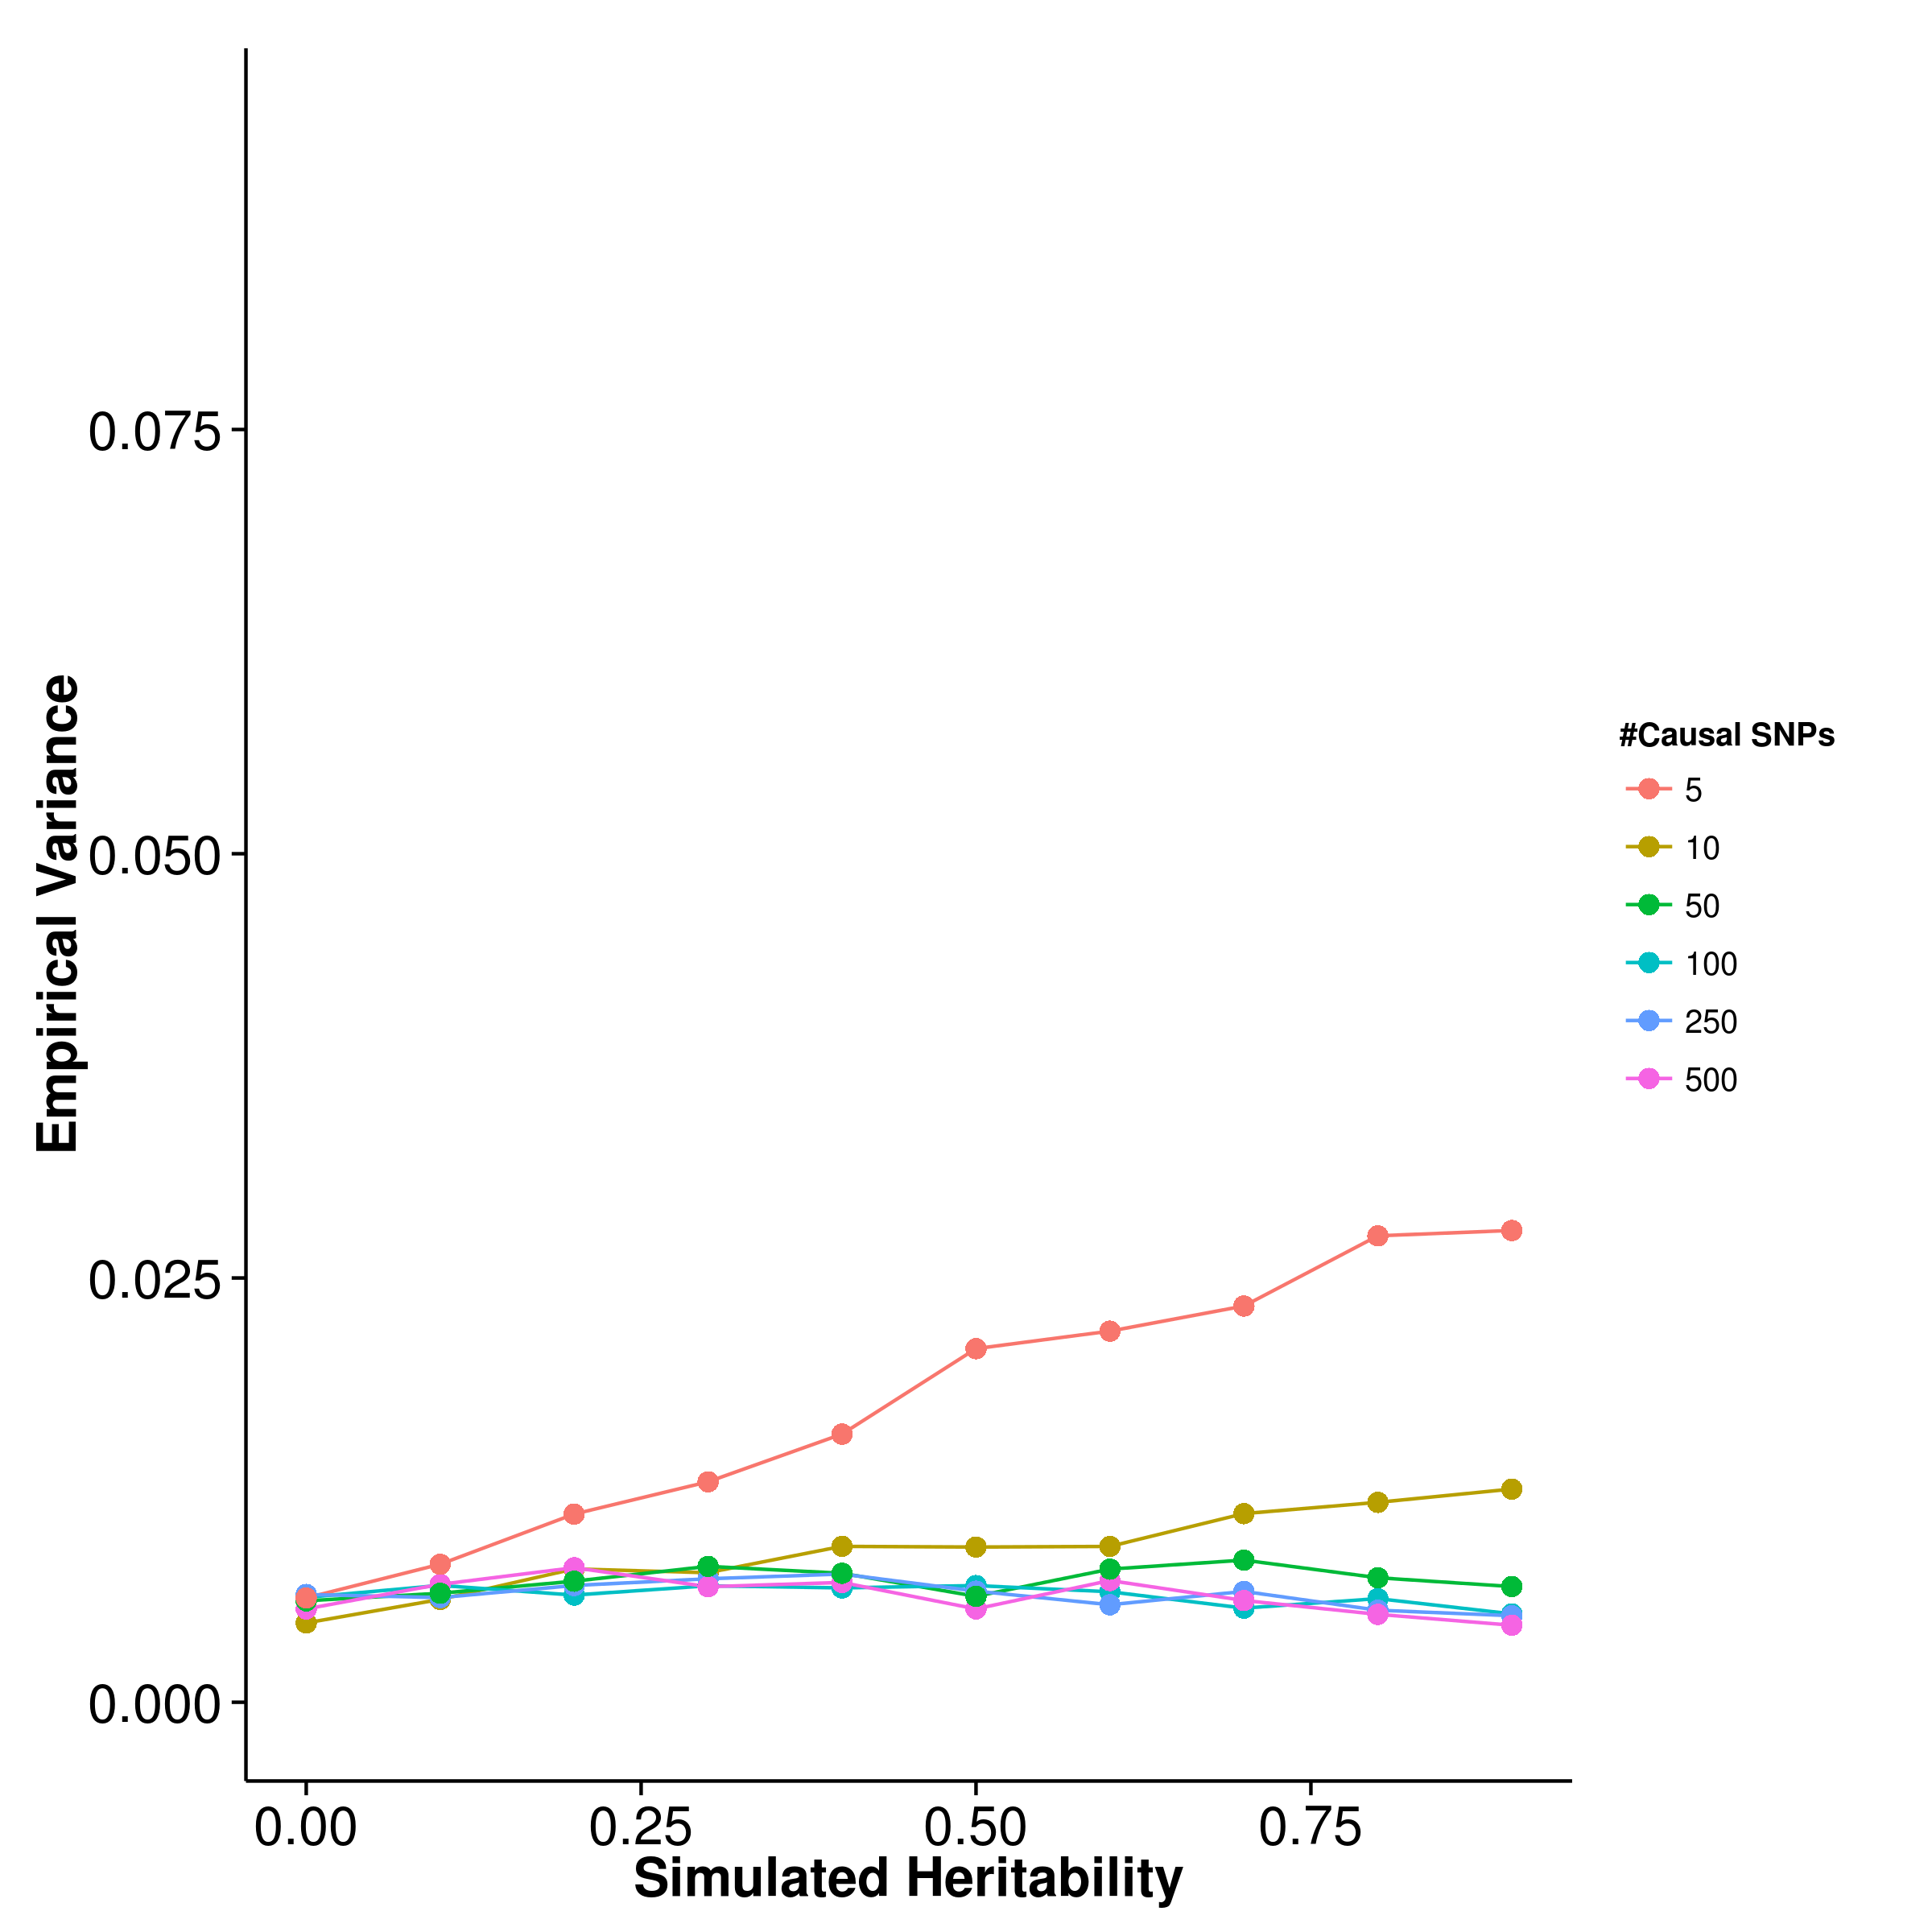
\includegraphics{figure/he_summary/equal/gcta_Qt_Equal_sd.png}}
				\label{fig:gctaQtEqualVar}
			}\\
			\subfloat[LDSC with fix intercept]{
				\scalebox{.4}{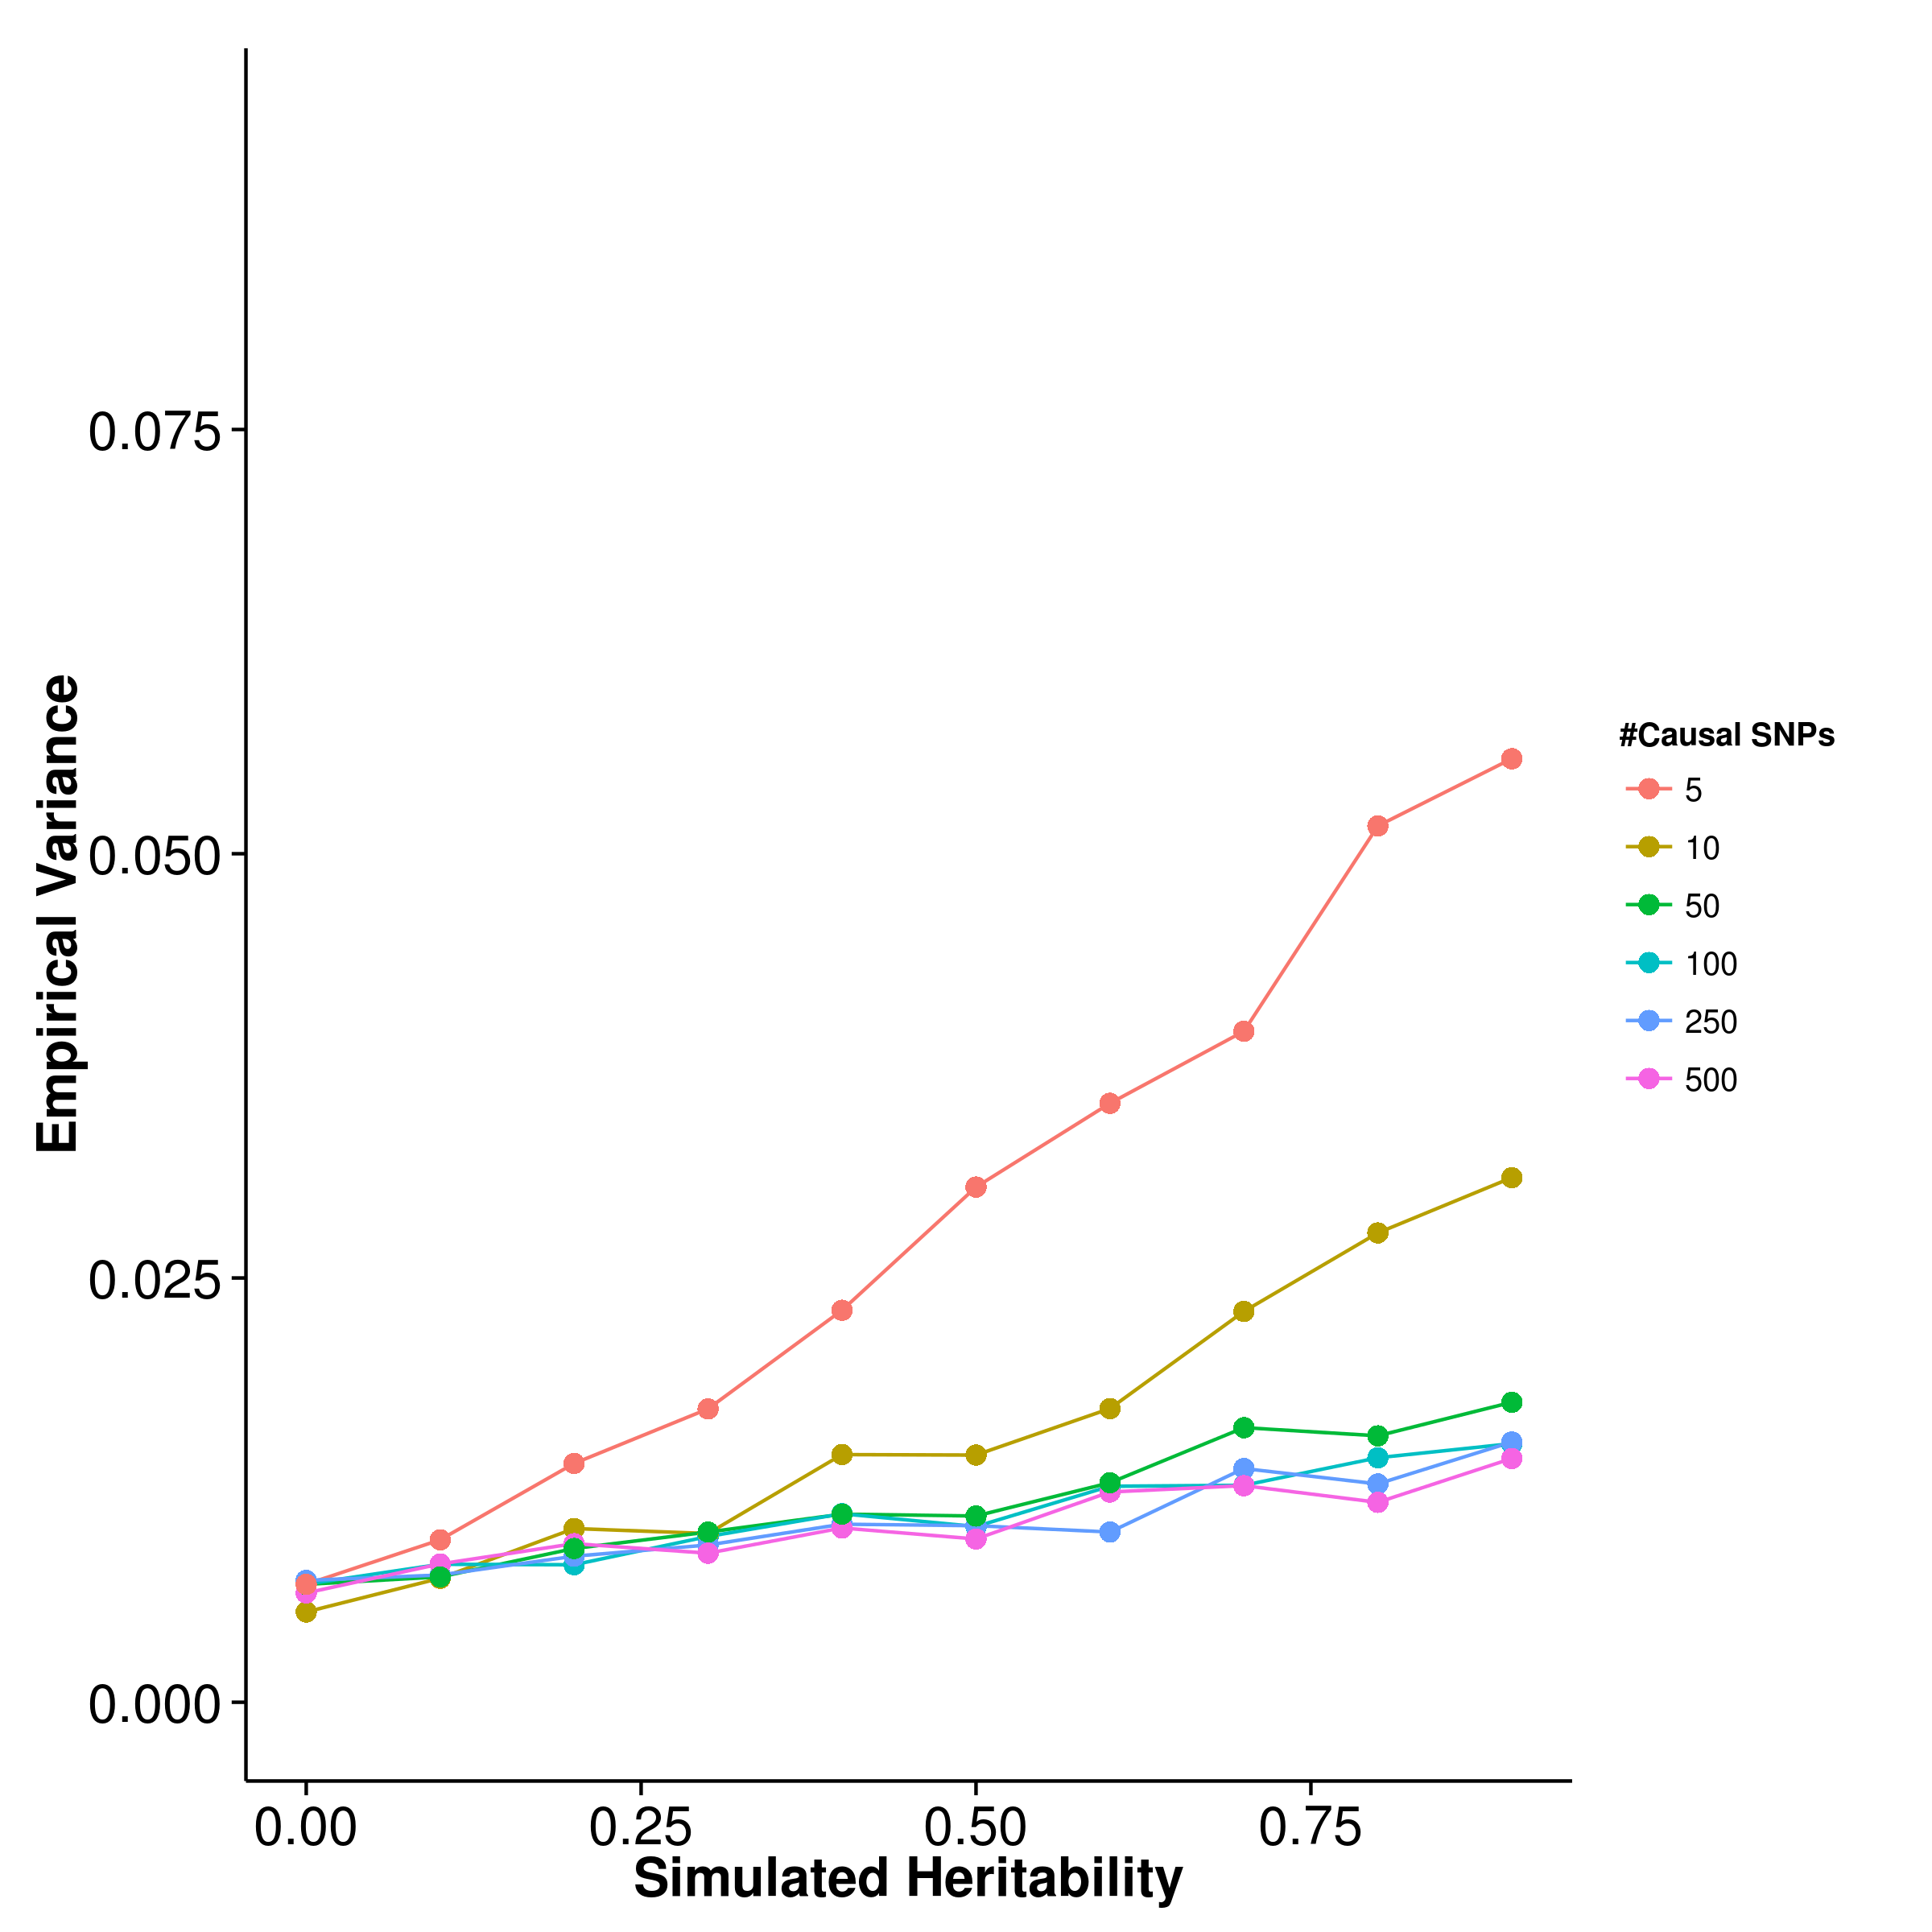
\includegraphics{figure/he_summary/equal/ldsc_Qt_Equal_sd.png}}
				\label{fig:ldscQtEqualVar}
			}
			\subfloat[LDSC with intercept estimation]{
				
				\scalebox{.4}{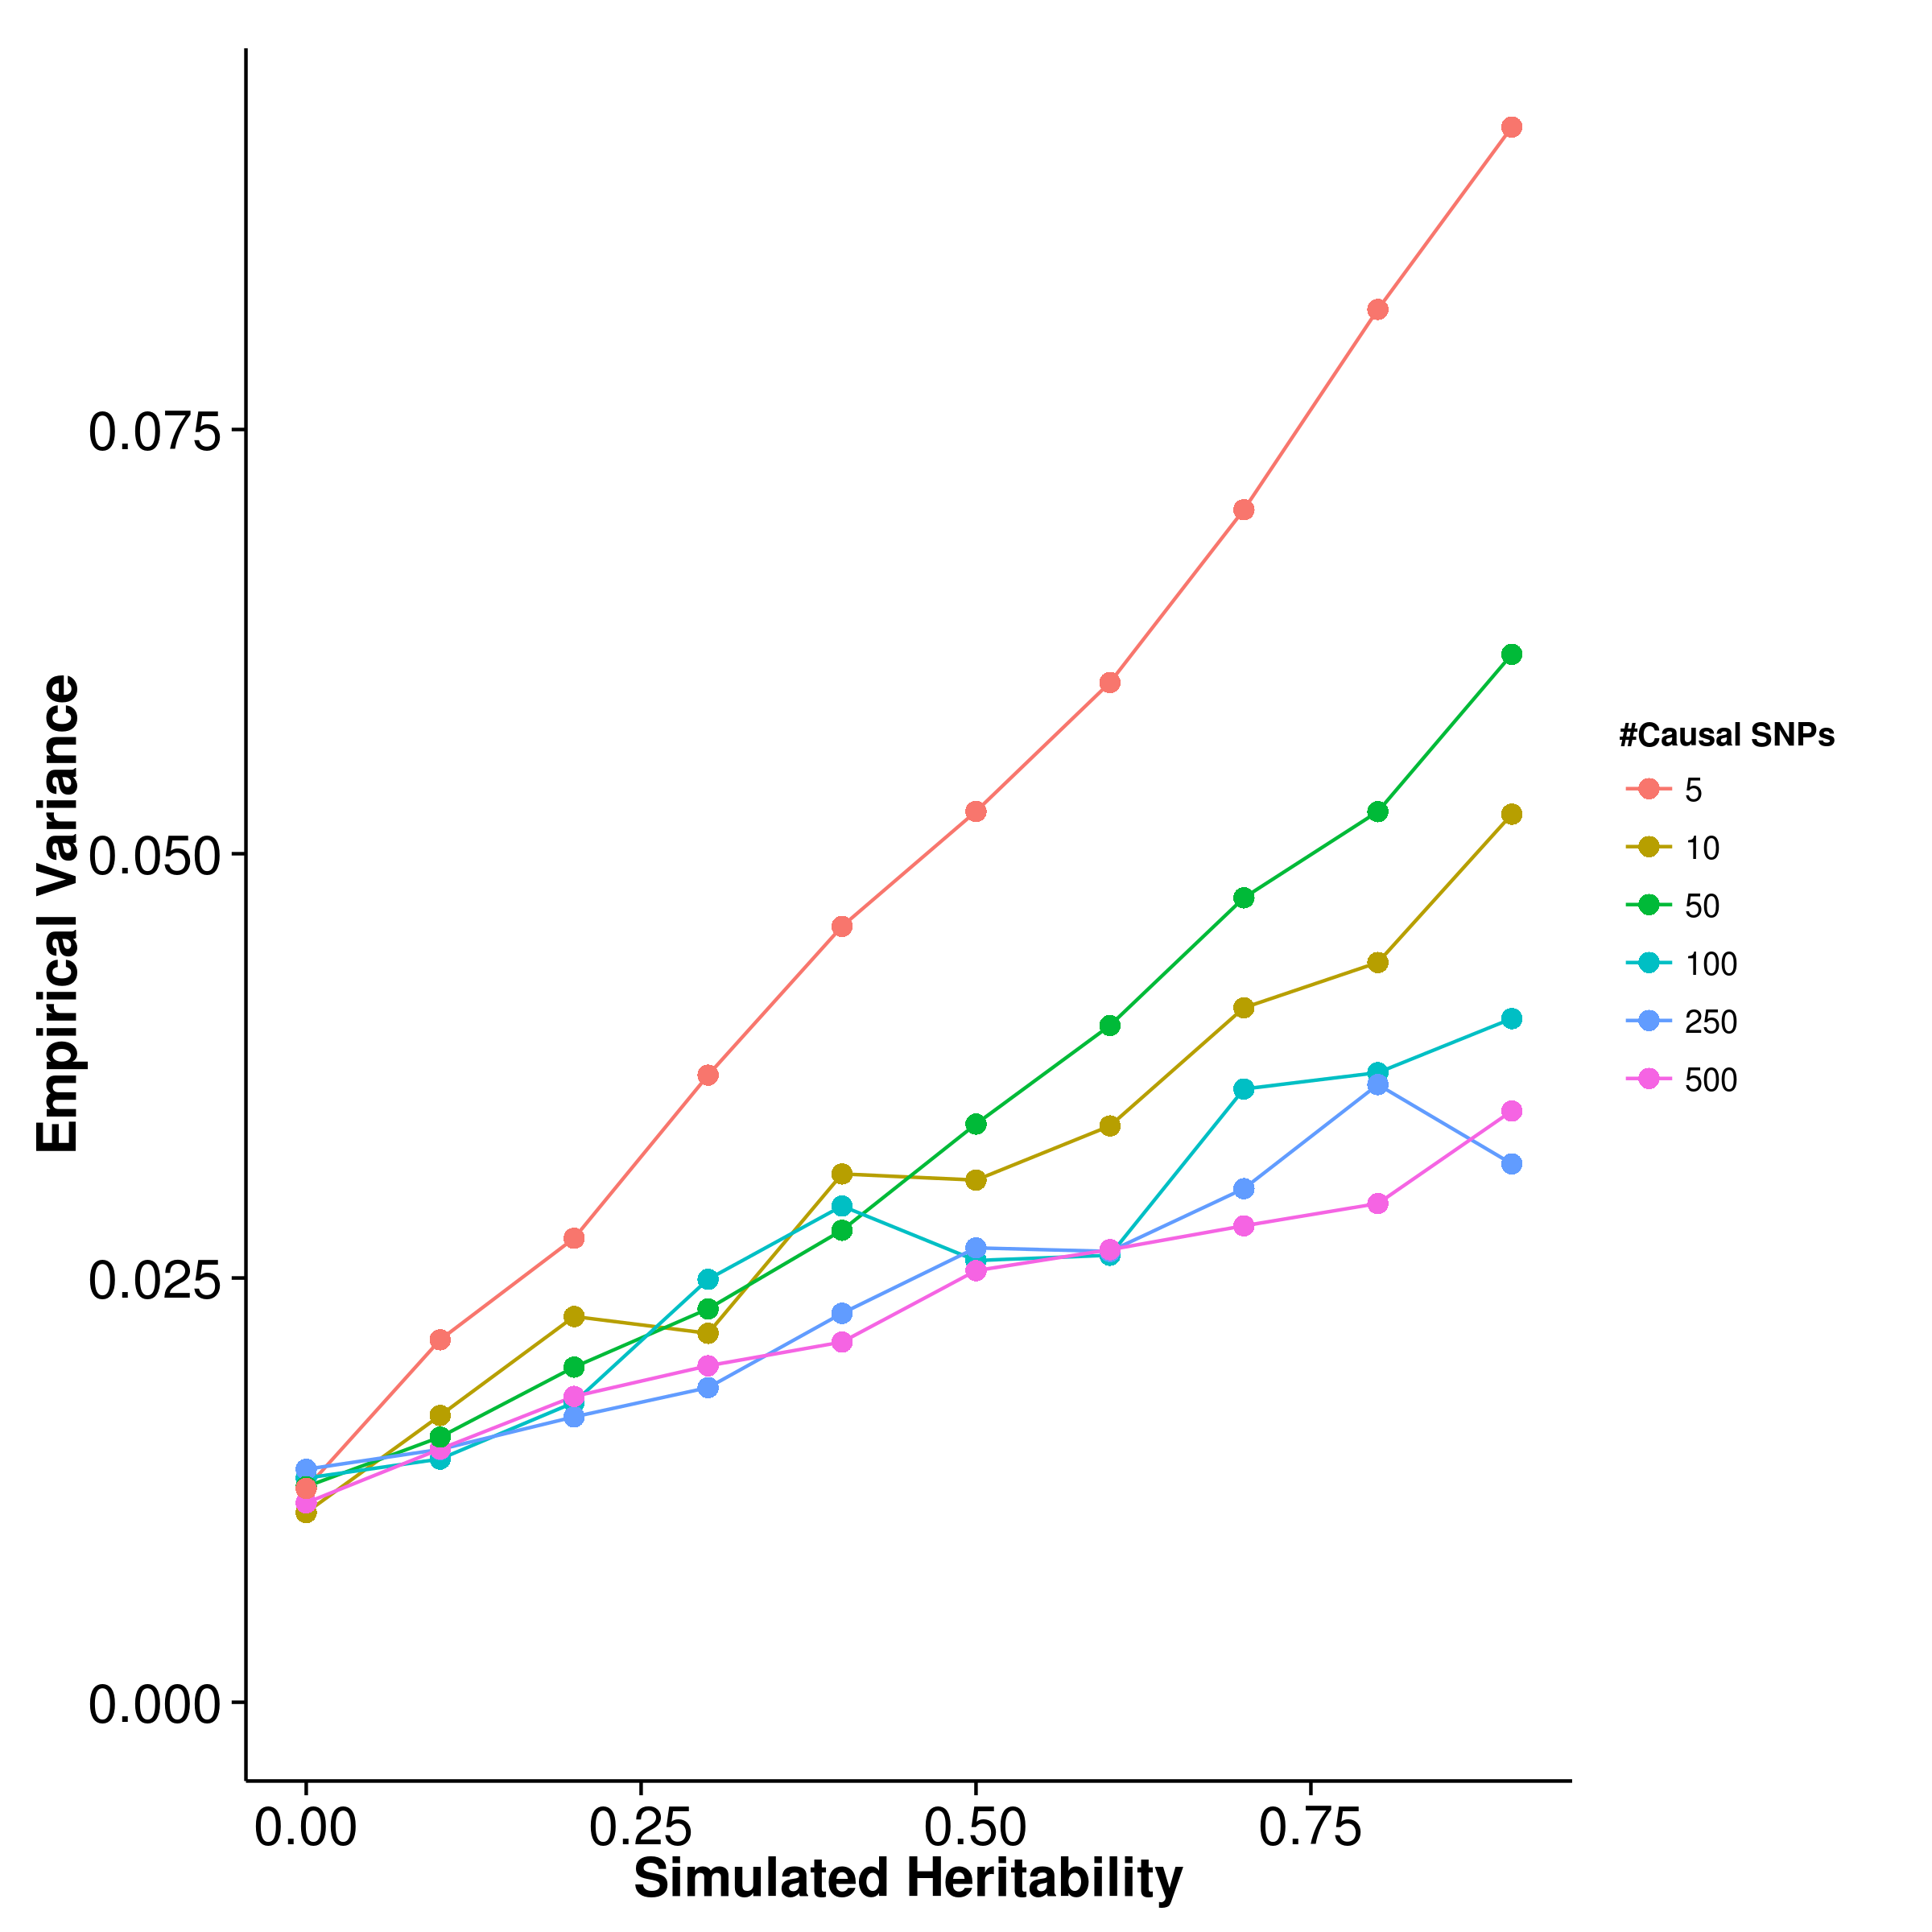
\includegraphics{figure/he_summary/equal/ldscIn_Qt_Equal_sd.png}}
				\label{fig:ldscInQtEqualVar}
			}
			\caption[Quantitative Trait with Equal Effect Size Simulation Result(Variance)]
			{Variance of results from quantitative trait simulation with equal effect size simulation.
				Of all the programmes, \gls{gcta} was found to have the lowest variance, follow by \gls{ldsc} with fixed intercept.
				The variance of \gls{shrek} was slightly higher than that of \gls{ldsc} with fixed intercept and is lower than that of \gls{ldsc} with intercept estimation.
				Unlike \gls{ldsc}, the variance of \gls{shrek} was less sensitive to change in total heritability.} 
			\label{fig:QtEqualVar}
		\end{figure}
		
		\begin{figure}
			\centering
			\subfloat[SHREK]{
				\scalebox{.4}{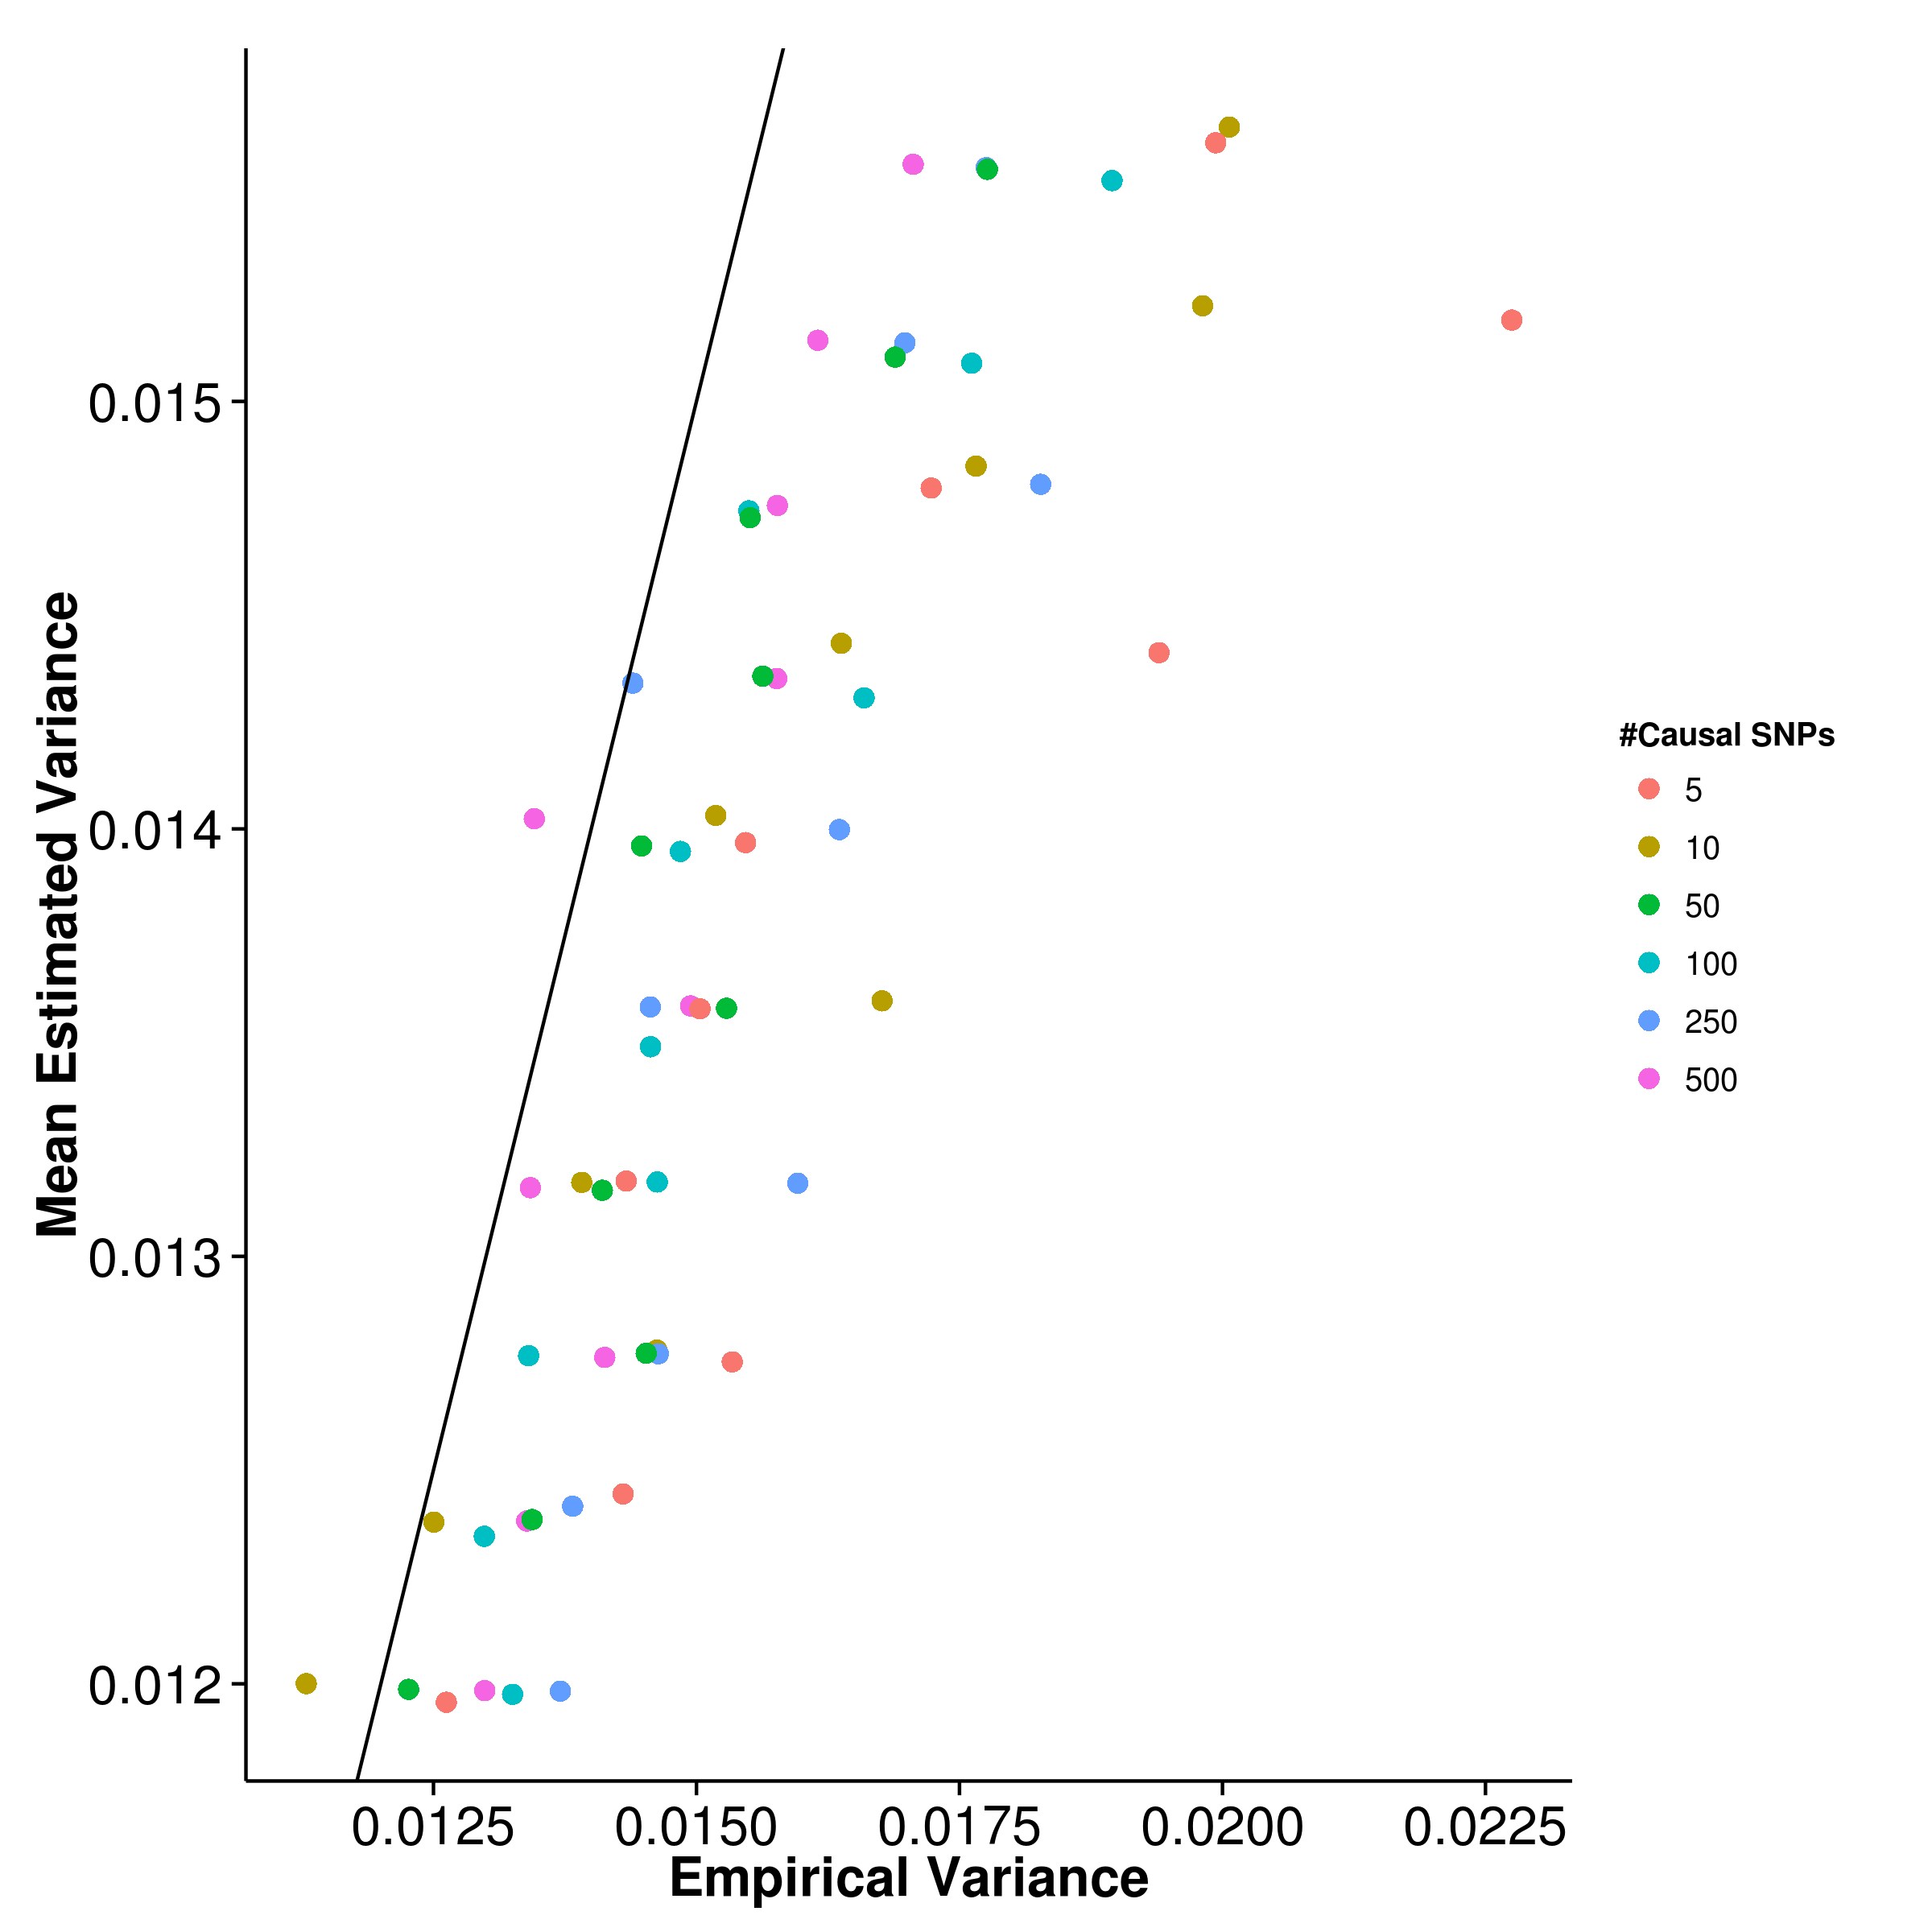
\includegraphics{figure/he_summary/equal/shrek_Qt_Equal_sdCom.png}}
				\label{fig:shrekQtEqualVarCom}
			}
			\subfloat[GCTA]{
				\scalebox{.4}{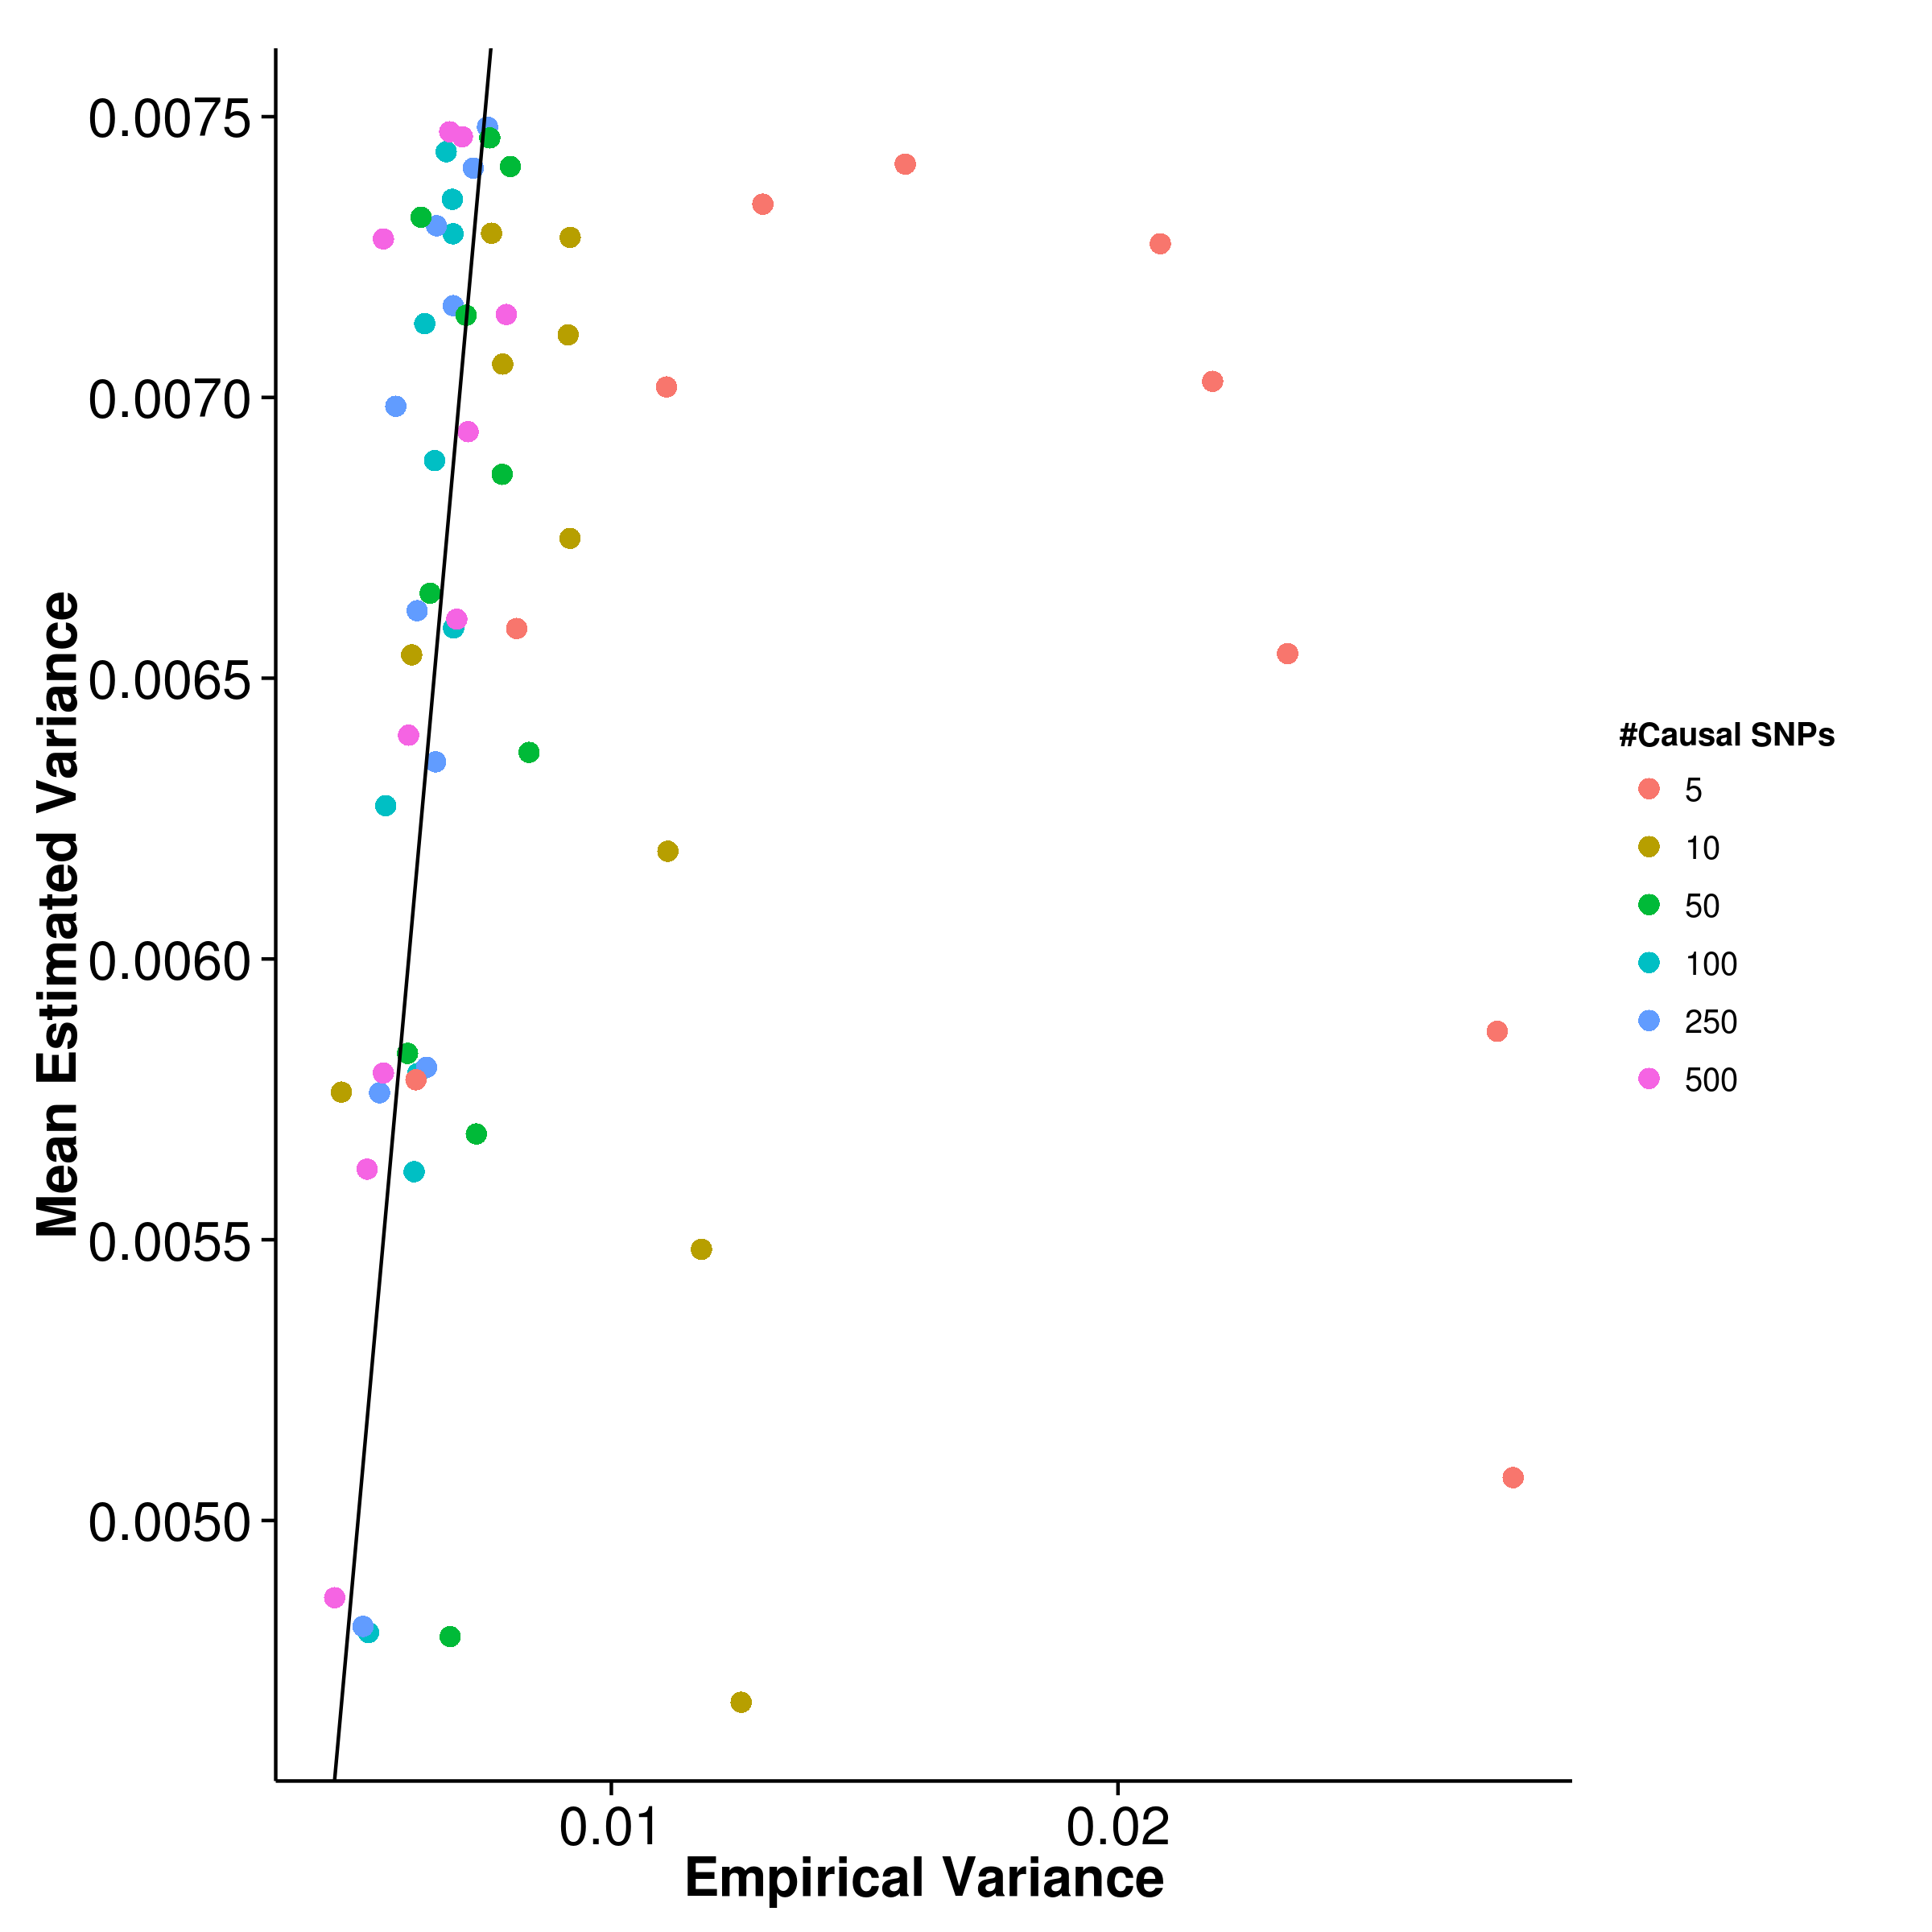
\includegraphics{figure/he_summary/equal/gcta_Qt_Equal_sdCom.png}}
				\label{fig:gctaQtEqualVarCom}
			}\\
			\subfloat[LDSC with fix intercept]{
				\scalebox{.4}{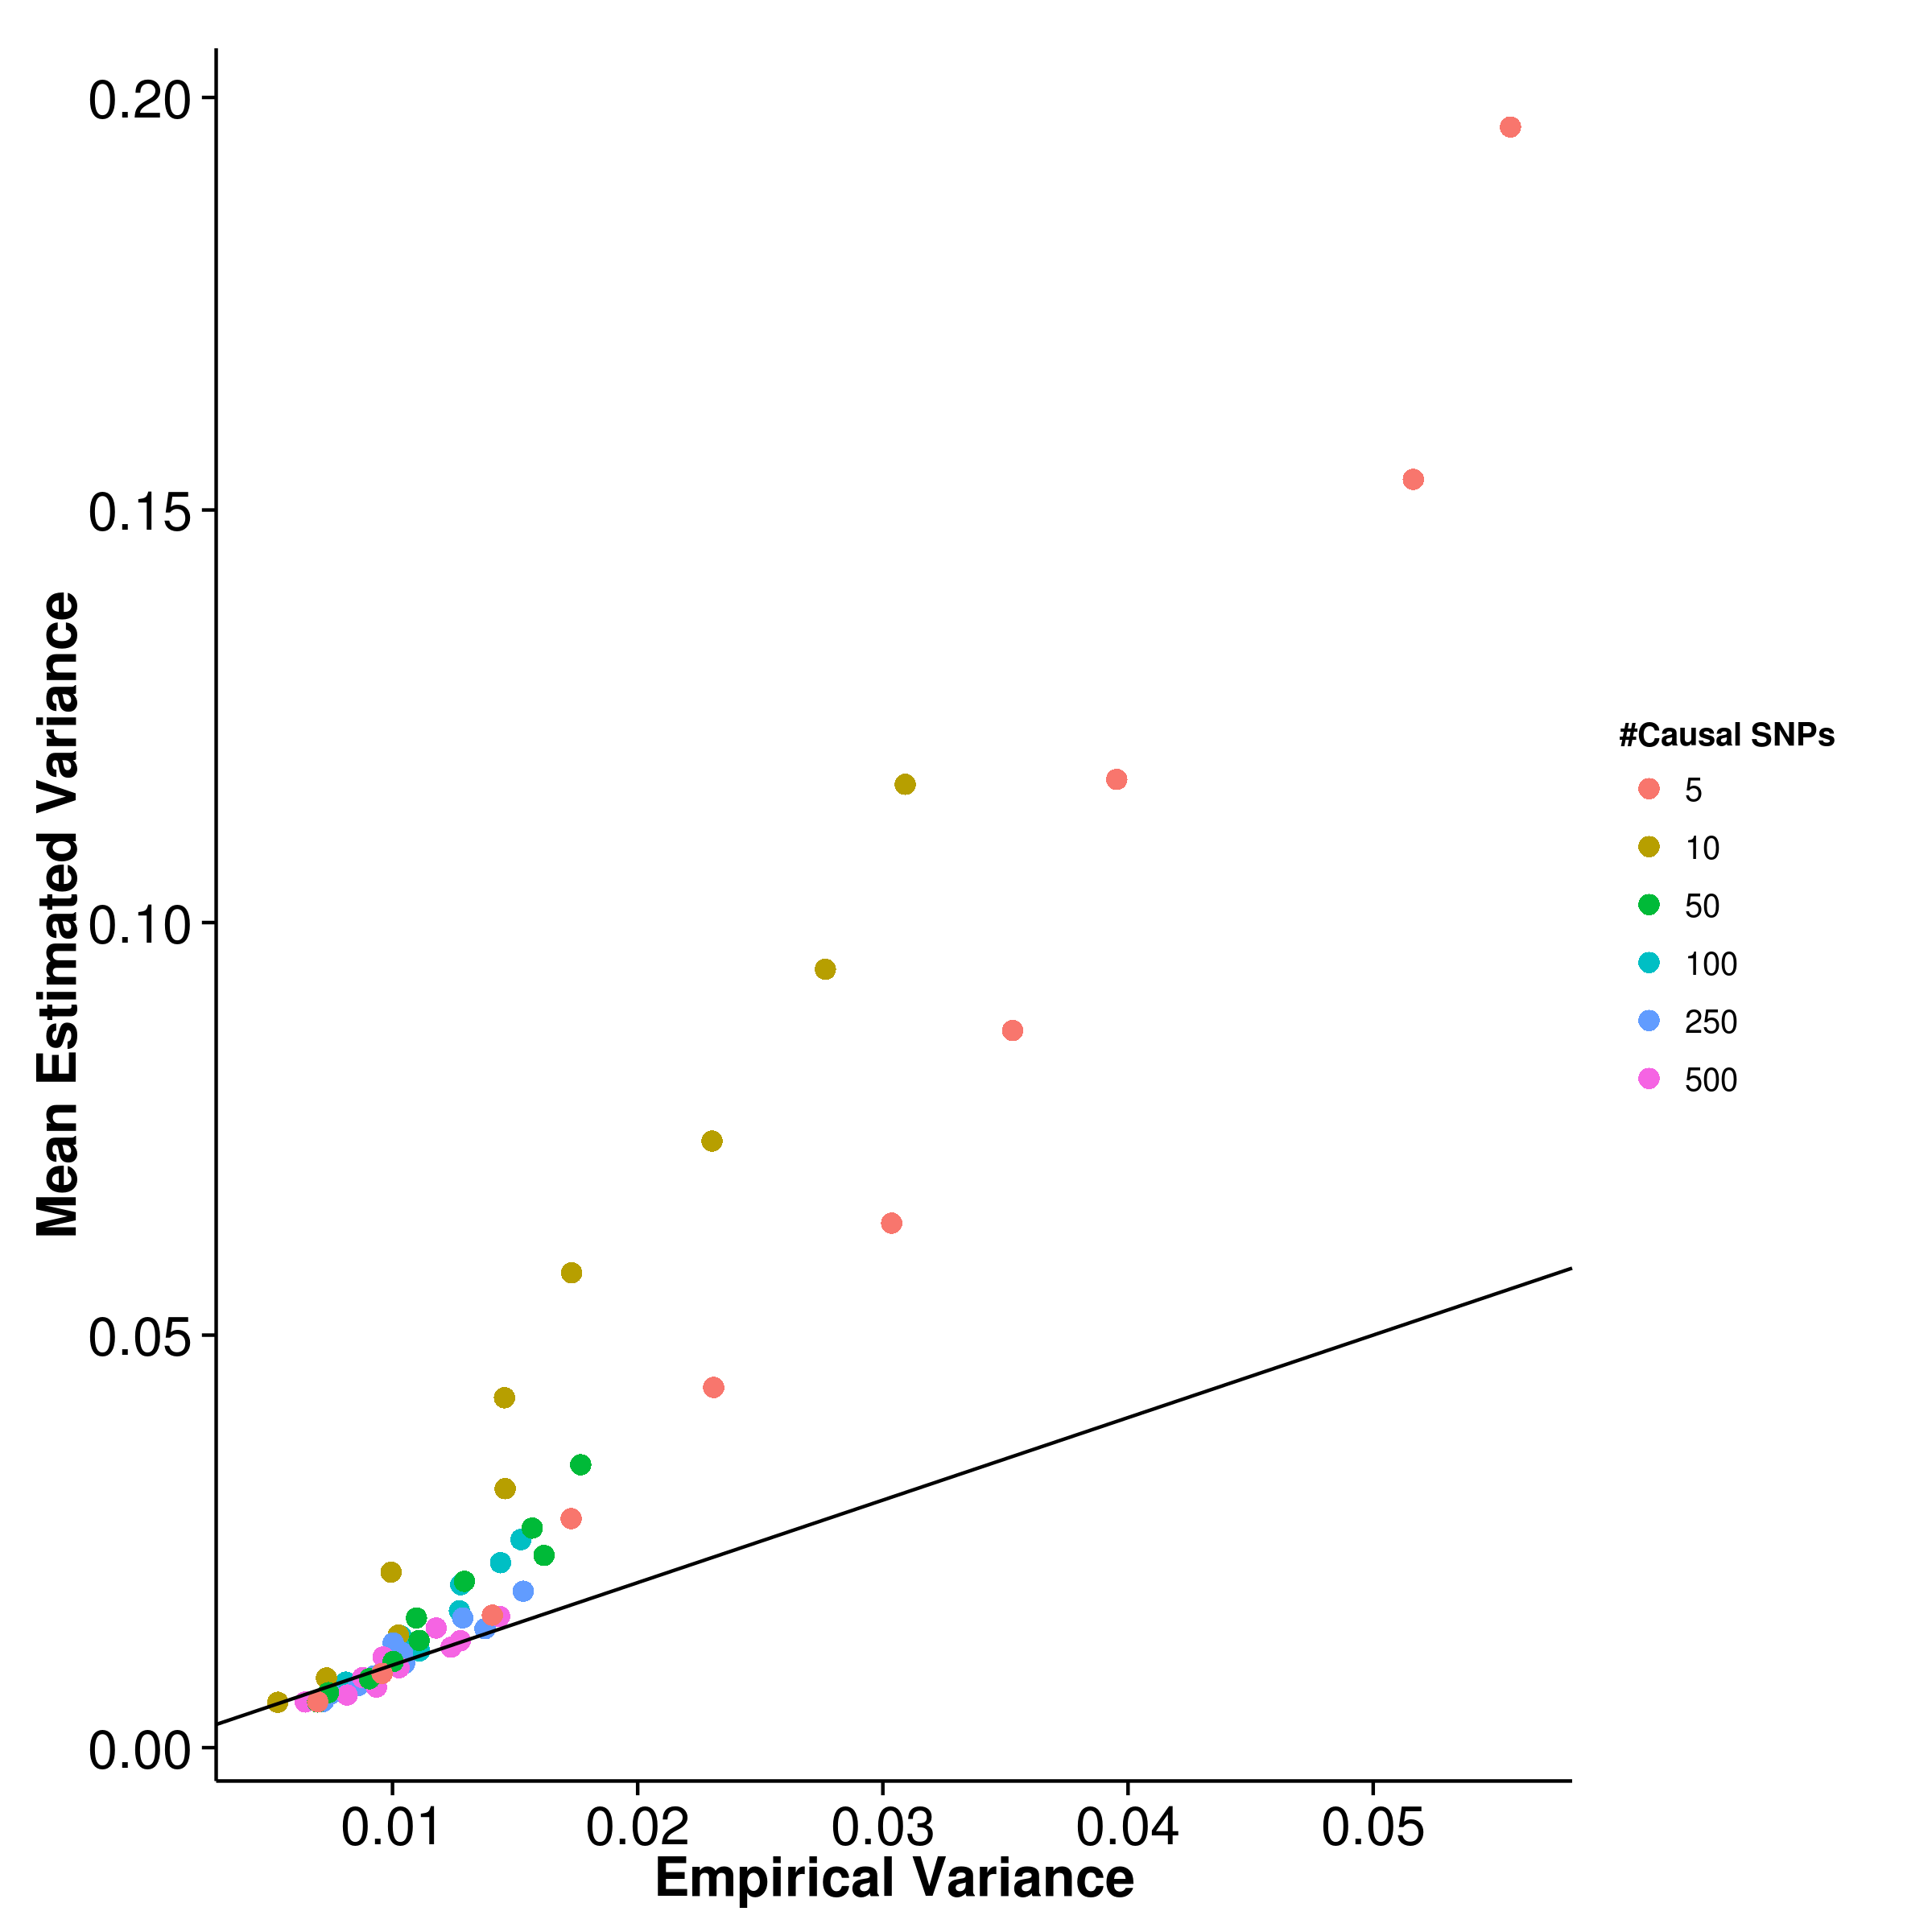
\includegraphics{figure/he_summary/equal/ldsc_Qt_Equal_sdCom.png}}
				\label{fig:ldscQtEqualVarCom}
			}
			\subfloat[LDSC with intercept estimation]{
				
				\scalebox{.4}{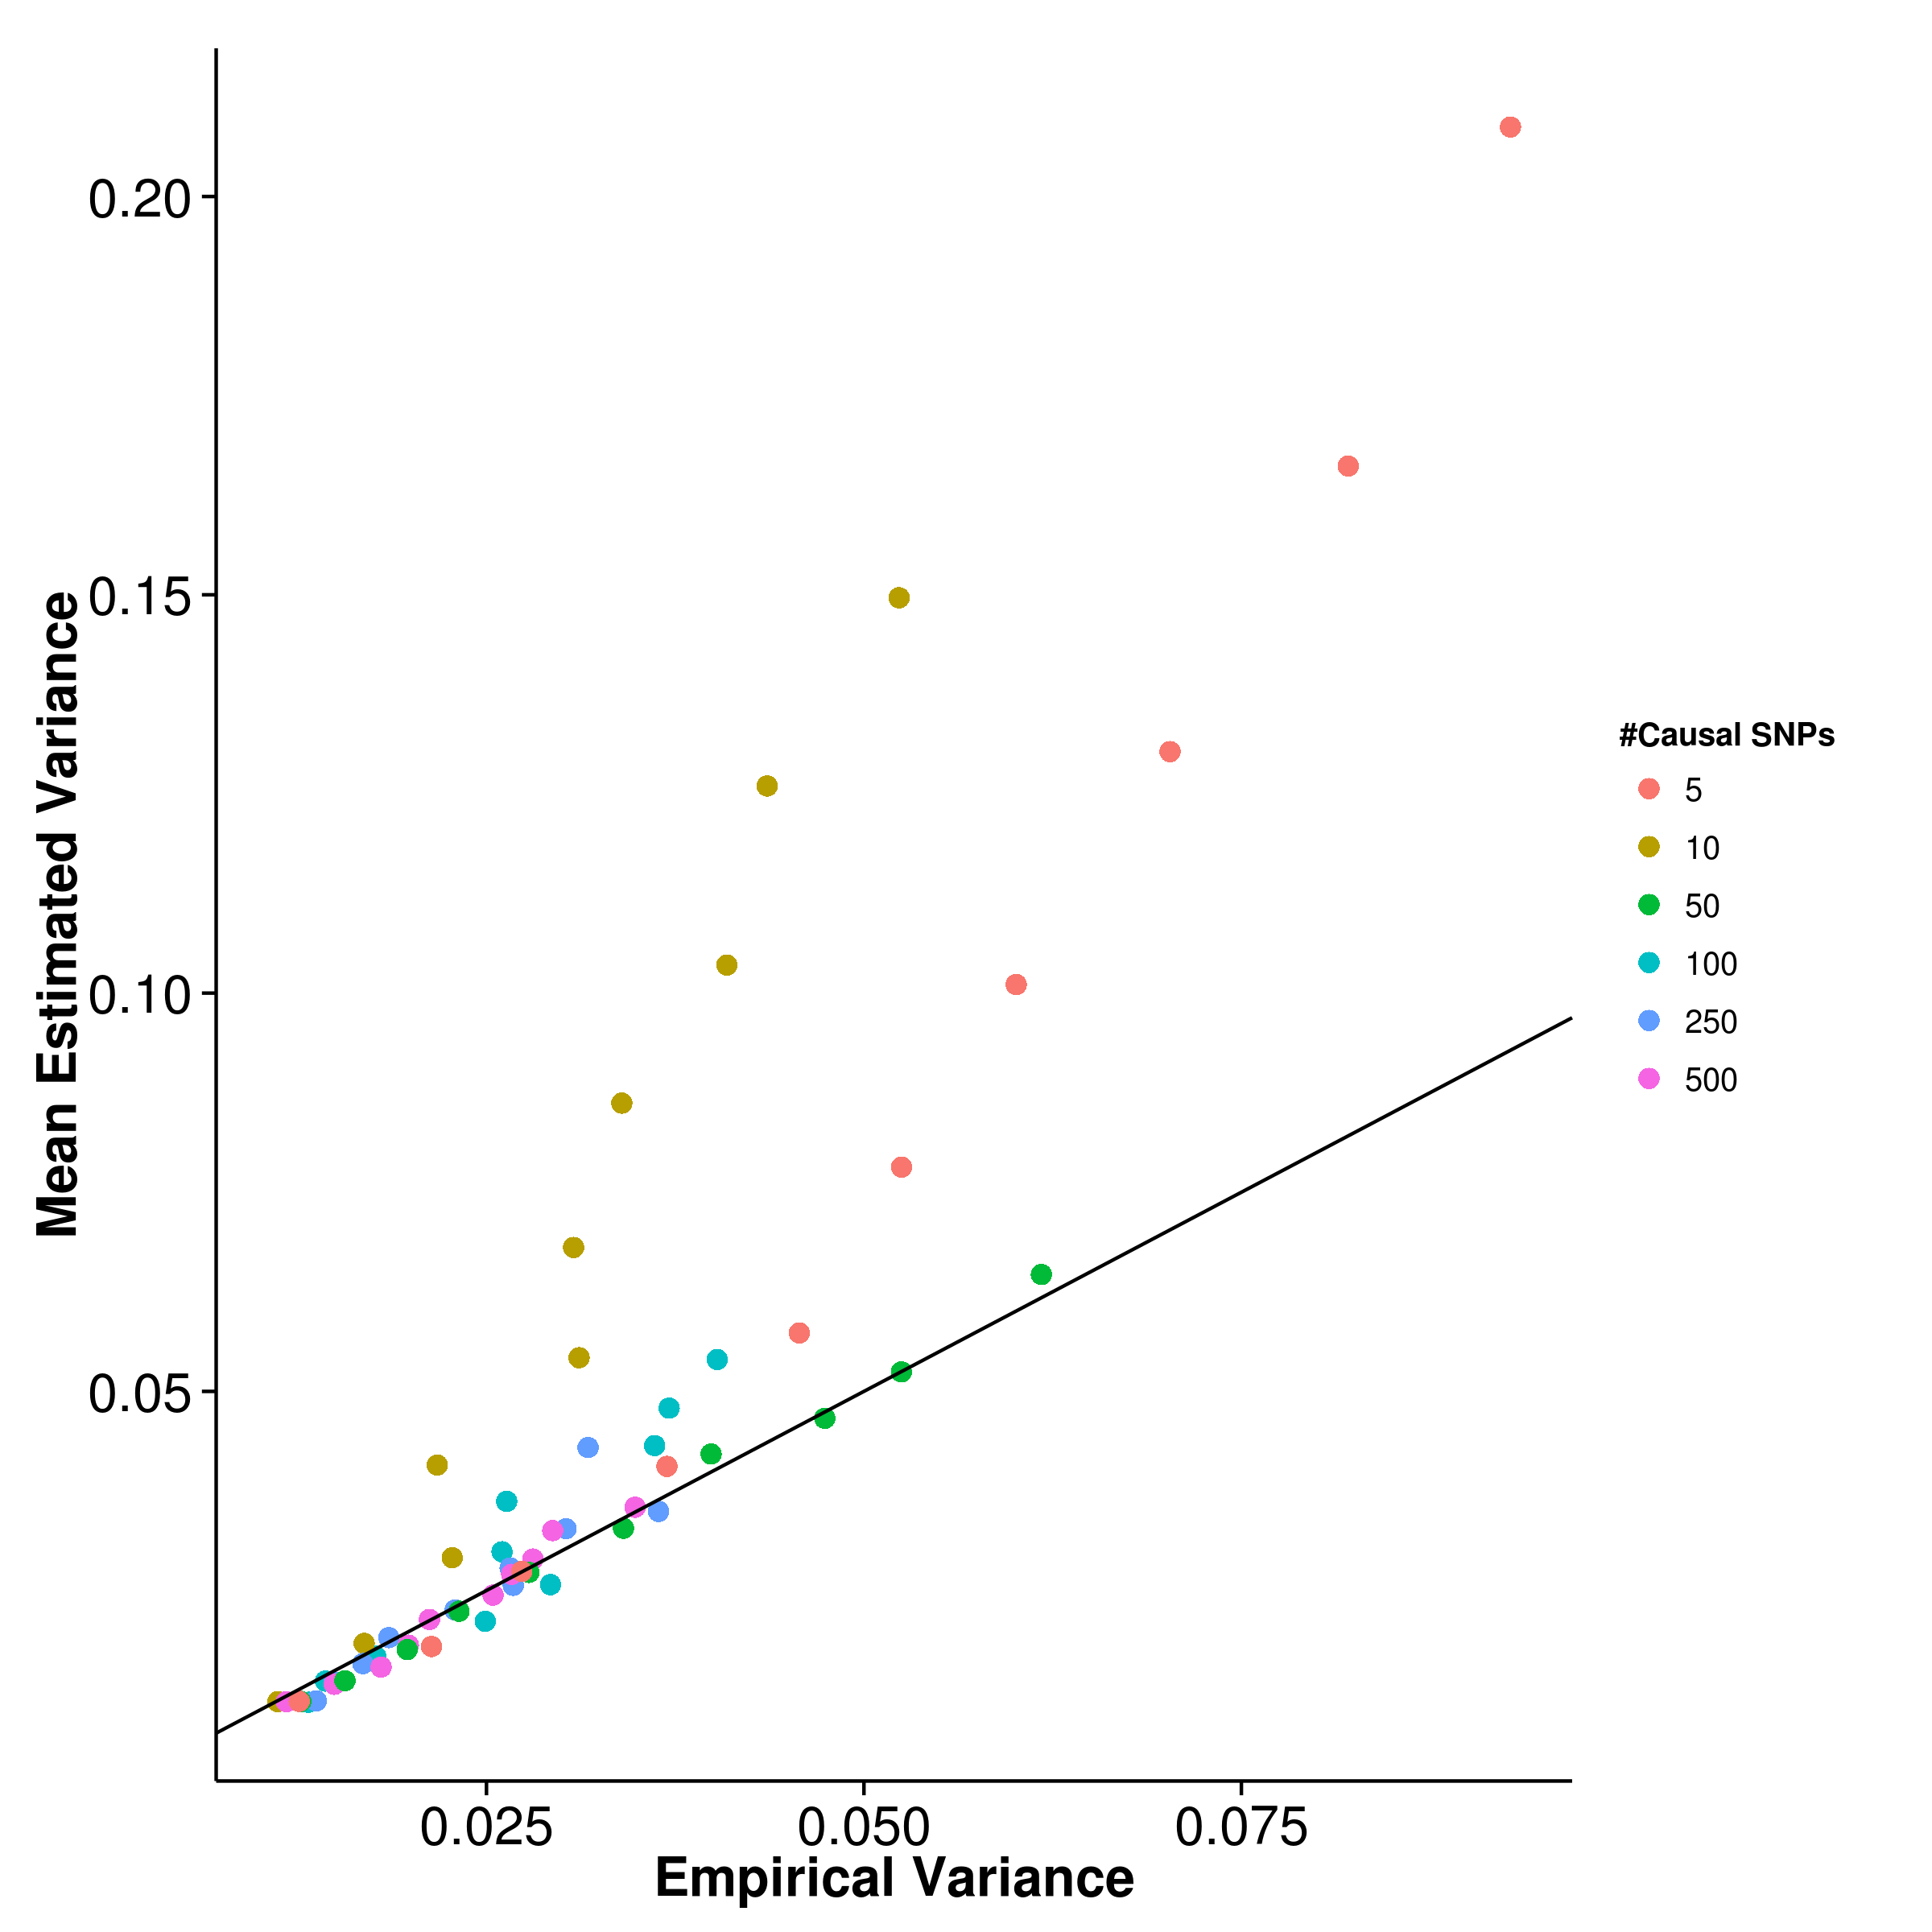
\includegraphics{figure/he_summary/equal/ldscIn_Qt_Equal_sdCom.png}}
				\label{fig:ldscInQtEqualVarCom}
			}
			\caption[Quantitative Trait with Equal Effect Size Simulation Result(Estimated Variance)]
			{Estimated variance of results from quantitative trait simulation with equal effect size simulation compared to the empirical variance.
				The estimated variances of all the tools were rather sensitive to the number of causal \glspl{SNP}, where \gls{ldsc} tends to over-estimate the variance as the number of causal \glspl{SNP} decreases and \gls{shrek} and \gls{gcta} tends to under-estimate the variance.} 
			\label{fig:QtEqualVarCom}
		\end{figure}
		The simulation of equal effect size serves as a simplistic baseline model for the performance of the programmes.
		The first thing to look at is the mean estimation of heritability of the programmes.
		If there is any bias in the estimation of the programmes, one can easily visualize it by plotting the mean estimated heritability against the simulated heritability(\cref{fig:QtEqualMean}).
		
		From the graph, it is clear that there was a slight over estimation for \gls{ldsc} with fixed intercept(\cref{fig:ldscQtEqualMean}).
		The over estimation seems to be a function of the simulated heritability, where a large inflation was observed when a larger heritability was simulated.
		On the other hand, when allow for the estimation of intercept, less bias was observed for \gls{ldsc} except for the scenario where only 5 causal \glspl{SNP} was simulated where the estimation was downwardly biased.
		
		Comparing to \gls{ldsc}, \gls{shrek} has a smaller bias and tends to slightly under-estimate(\cref{fig:shrekQtEqualMean}).
		However, the bias of \gls{shrek} is insensitive to the simulated heritability, making it robust to traits with different heritability.
		Similarly, the bias of \gls{gcta} is also smaller than that of \gls{ldsc}(\cref{fig:shrekQtEqualMean}), with a slight upward bias in the estimation except when 5 causal \glspl{SNP} was simulated.
		Again, the estimate of \gls{gcta} is also relatively insensitive to the simulated heritability.
		Overall, there was no clear pattern as to how the number of causal \glspl{SNP} affects the mean estimation. 
		
		Next, we examine the empirical variance of the programmes(\cref{fig:QtEqualVar}).
		As can be seen from the graph, there is a clear pattern where the decrease in number of causal \gls{SNP} generally increases the variance for all the programmes, with \gls{shrek} least affected.
		For \gls{ldsc}, the simulated heritability also have a large impact to its empirical variance, with the empirical variance increases as the simulated heritability increases.
		In general, \gls{ldsc} with fixed intercept(\cref{fig:ldscQtEqualVar}) has a lower variance when compared to \gls{ldsc} with intercept estimation(\cref{fig:ldscInQtEqualVar}). 
		Moreover, when the number of causal \gls{SNP} is large, the variance of \gls{ldsc} with fixed intercept(\cref{fig:ldscQtEqualVar}) is lower than \gls{shrek}(\cref{fig:shrekQtEqualVar}).
		However, \gls{shrek} is more robust to change in the number of causal \glspl{SNP} and simulated heritabiliy when compared ot \gls{ldsc}.

		Of all the programmes, \gls{gcta} has the best performance(\cref{fig:gctaQtEqualVar}) except when the trait only contains 5 causal \glspl{SNP}. 
		Not only does it has the smallest variance, its empirical variances was almost invariant to change in simulated heritability.
		However, the case with 5 causal \glspl{SNP} serves as an out-lier. 
		It was most obvious when inspecting the relationship between the estimated variance and the empirical variance of \gls{gcta}(\cref{fig:gctaQtEqualVarCom}).
		Comparing the estimated variance and the empirical variance, it was clear that \gls{gcta} can, in most case accurately estimate its variance. 
		In the case of 5 causal \glspl{SNP} however, \gls{gcta} underestimates its variance.
		It was also observed in the case of 10 causal \glspl{SNP}, there was already a slight under-estimation of the variance, suggesting that there might be an increase in empirical variance that was not capture by \gls{gcta}.
		
		In the case of the programmes using the test statistic, it was observed that \gls{shrek} in general under-estimate the empirical variance(\cref{fig:shrekQtEqualVarCom}) for an average of 0.9 fold. 
		On the other hand, \gls{ldsc} over-estimates the variance for roughly 1.5 times when a fixed intercept(\cref{fig:ldscQtEqualVarCom}) was used and roughly 1.2 times when the intercept was estimated(\cref{fig:ldscInQtEqualVarCom}). 
		
		To summarize the results, we calculate the \gls{mse} of the estimation of heritability of the programmes under different simulation condition(\cref{tab:mseQtEqual}). 
		With the exception of the 5 causal \glspl{SNP} scenario, \gls{gcta} has the best performance, has a almost 2 fold smaller \gls{mse} when compared to \gls{shrek}.
		As the number of casual \glspl{SNP} increases, the performance of \gls{ldsc} with fixed intercept and \gls{shrek} converges where in general, \gls{shrek} has a smaller \gls{mse}.
		Interestingly, unlike \gls{ldsc}, \gls{shrek} was insensitive to change in number of causal \glspl{SNP} and its performance were relatively stable.
		
		% Describe the mean
		% Effect of heritability on the mean estimation
		% Effect of causal SNPs on the mean estimation
		% Descript the Variance
		% Effect of heritability on variance of estimate
		% Effect of number of causal SNPs on variance of estimation
		% Describe the estimated variance
		% How the number of causal SNPs affect the estimation of variance?

		\begin{table}
			\centering
			\begin{tabular}{rrrrr}
				\toprule
				Number of Causal SNPs&	SHREK&	LDSC&	LDSC-In&	GCTA \\
				\midrule
				5	&	0.167	&	0.308&	0.526&	0.177	\\
				10	&	0.158	&	0.243&	0.337&	0.0944	\\
				50	&	0.150	&	0.163&	0.354&	0.0749	\\
				100	&	0.154	&	0.161&	0.304&	0.0664	\\
				250	&	0.157	&	0.147&	0.255&	0.0659	\\
				500	&	0.147	&	0.148&	0.247&	0.0661	\\
				\bottomrule
			\end{tabular}
			\caption[Mean Squared Error of Quantitative Trait Simulation with Equal Effect Size]{
				\gls{mse} of quantitative trait simulation with equal effect size.
				It was observed that the overall \gls{mse} of \gls{gcta} is very low, follow by \gls{shrek}.
				As the number of causal \glspl{SNP} decreases, the \gls{mse} increases for all programmes. 
				The performance of \gls{shrek} and \gls{ldsc} with fixed intercept converges as the number of causal \glspl{SNP} increases.}
			\label{tab:mseQtEqual}
		\end{table}
		
		\subsection{Quantitative Trait Simulation with Random Effect Size}
		% QT Random Effect
			\begin{figure}
			\centering
			\subfloat[SHREK]{
				\scalebox{.4}{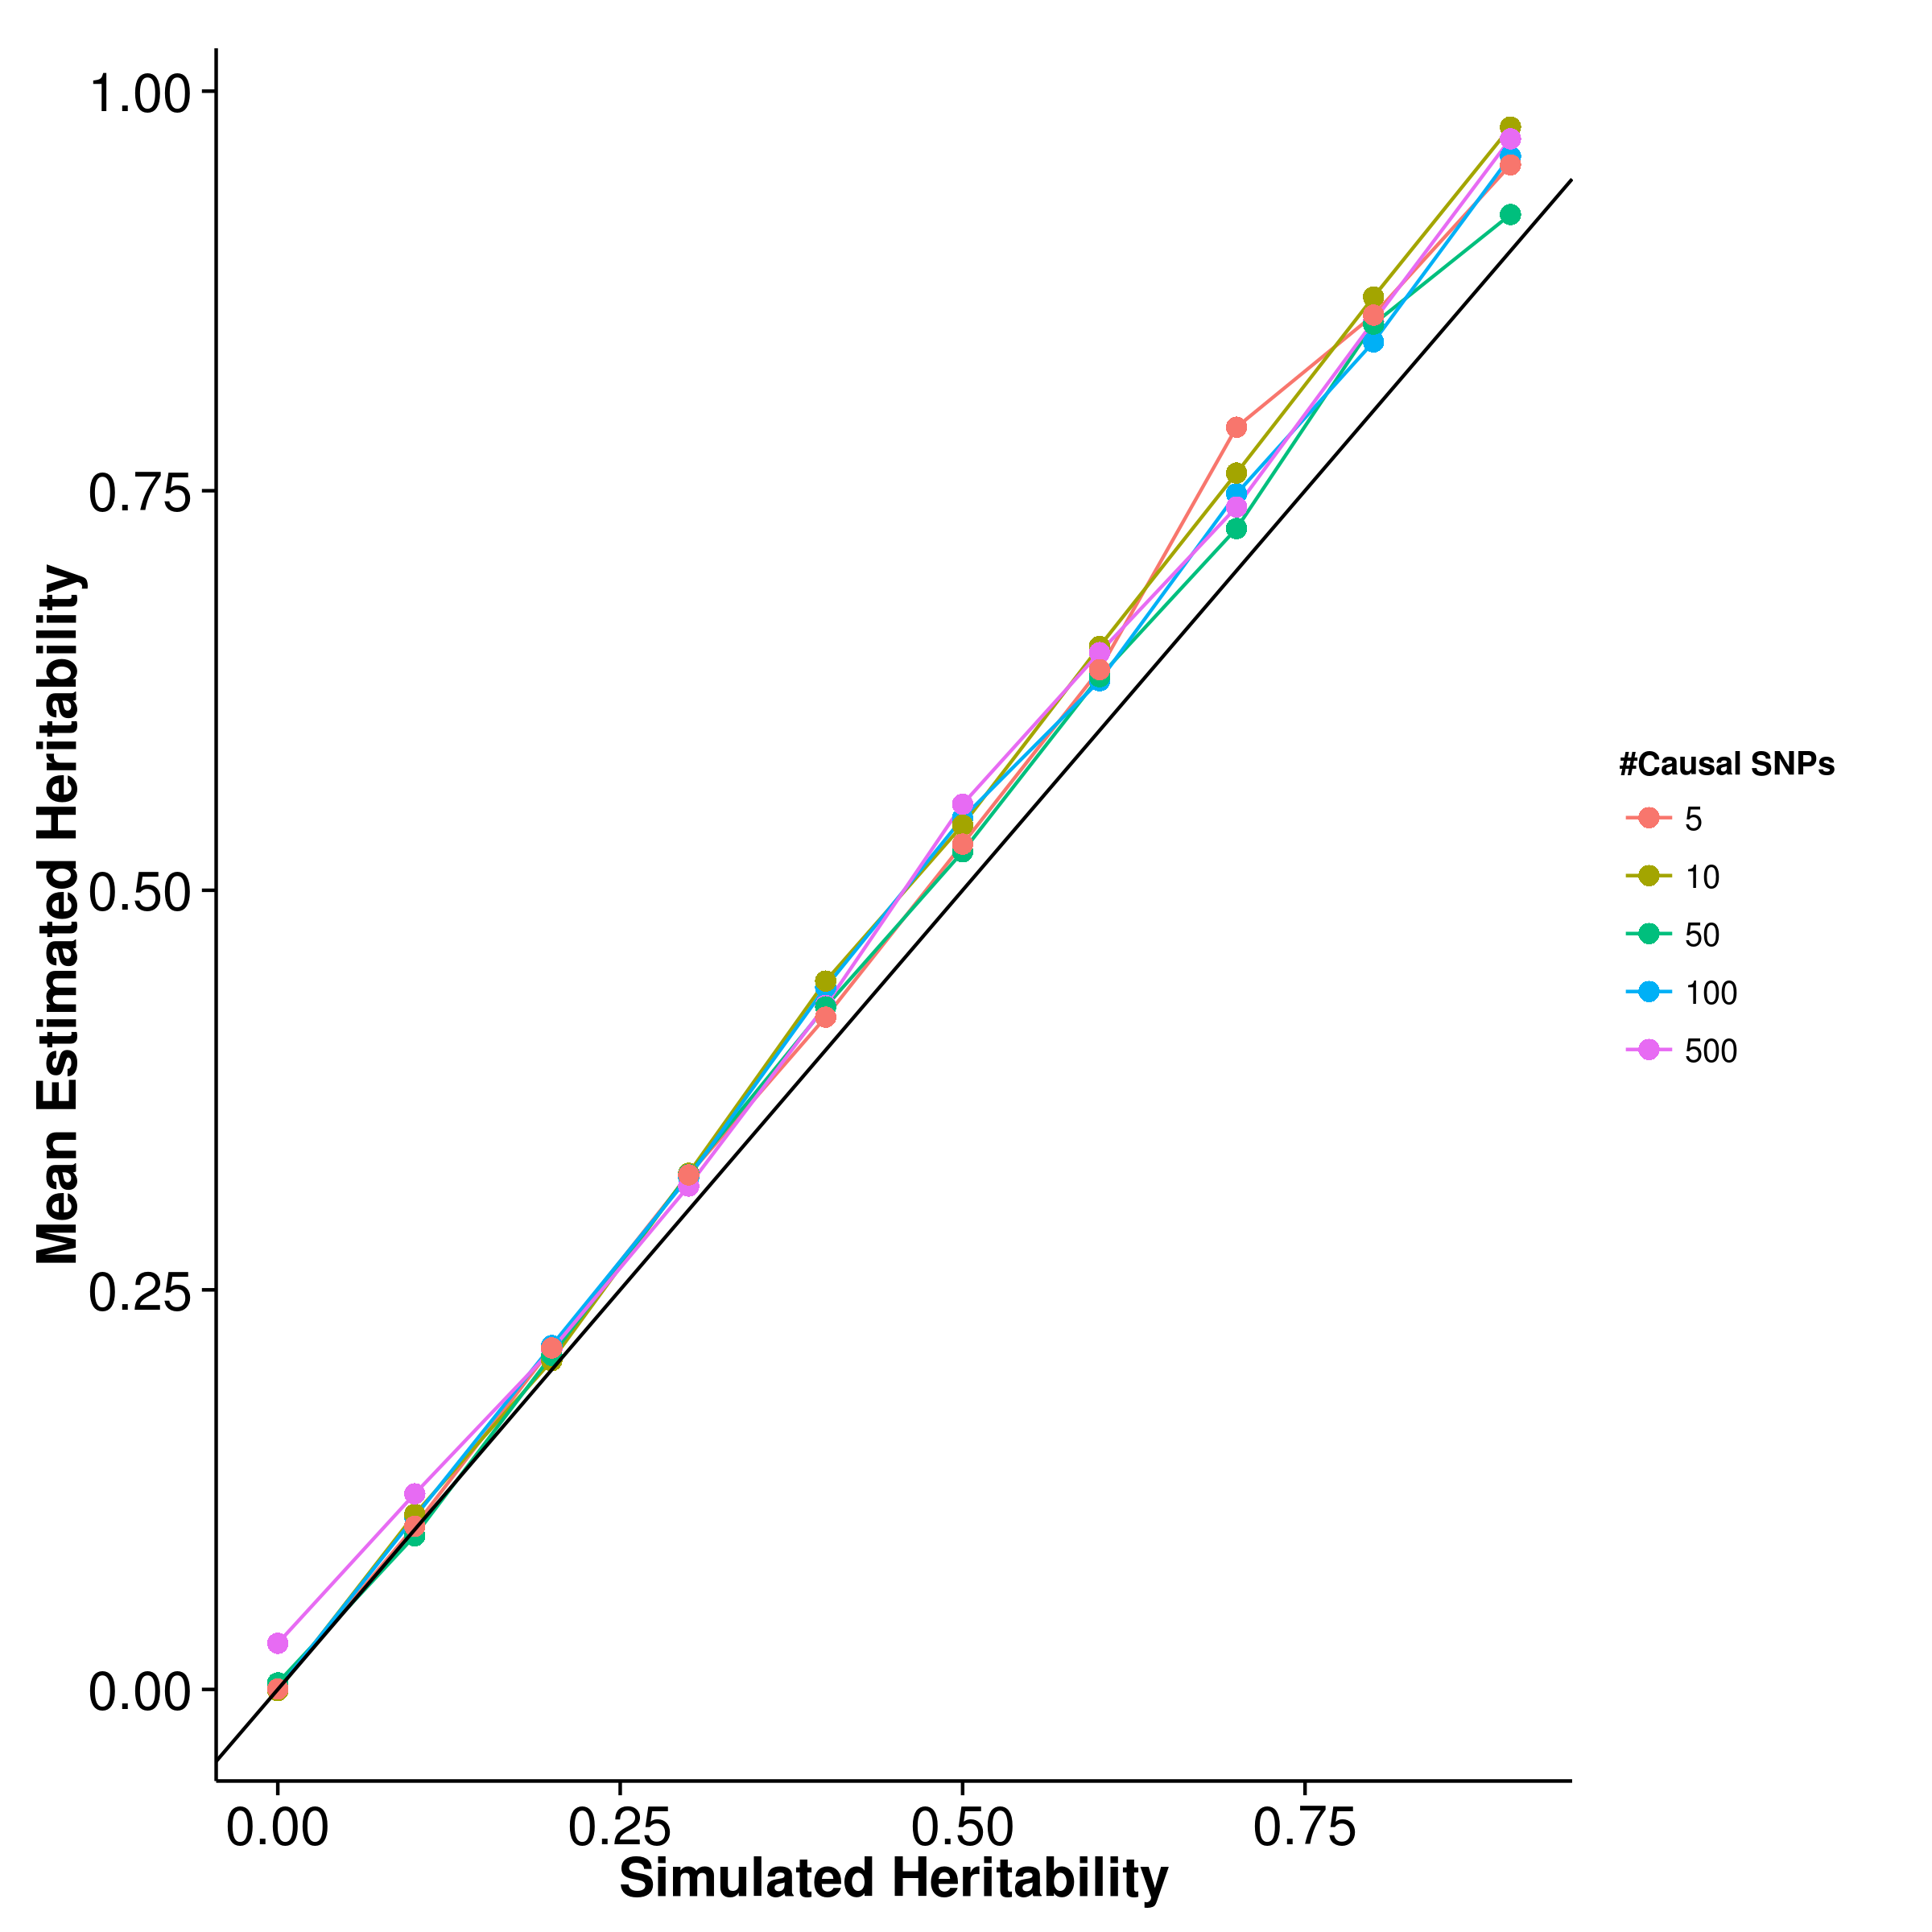
\includegraphics{figure/he_summary/random/shrek_Qt_Rand_mean.png}}
				\label{fig:shrekQtRandMean}
			}
			\subfloat[GCTA]{
				\scalebox{.4}{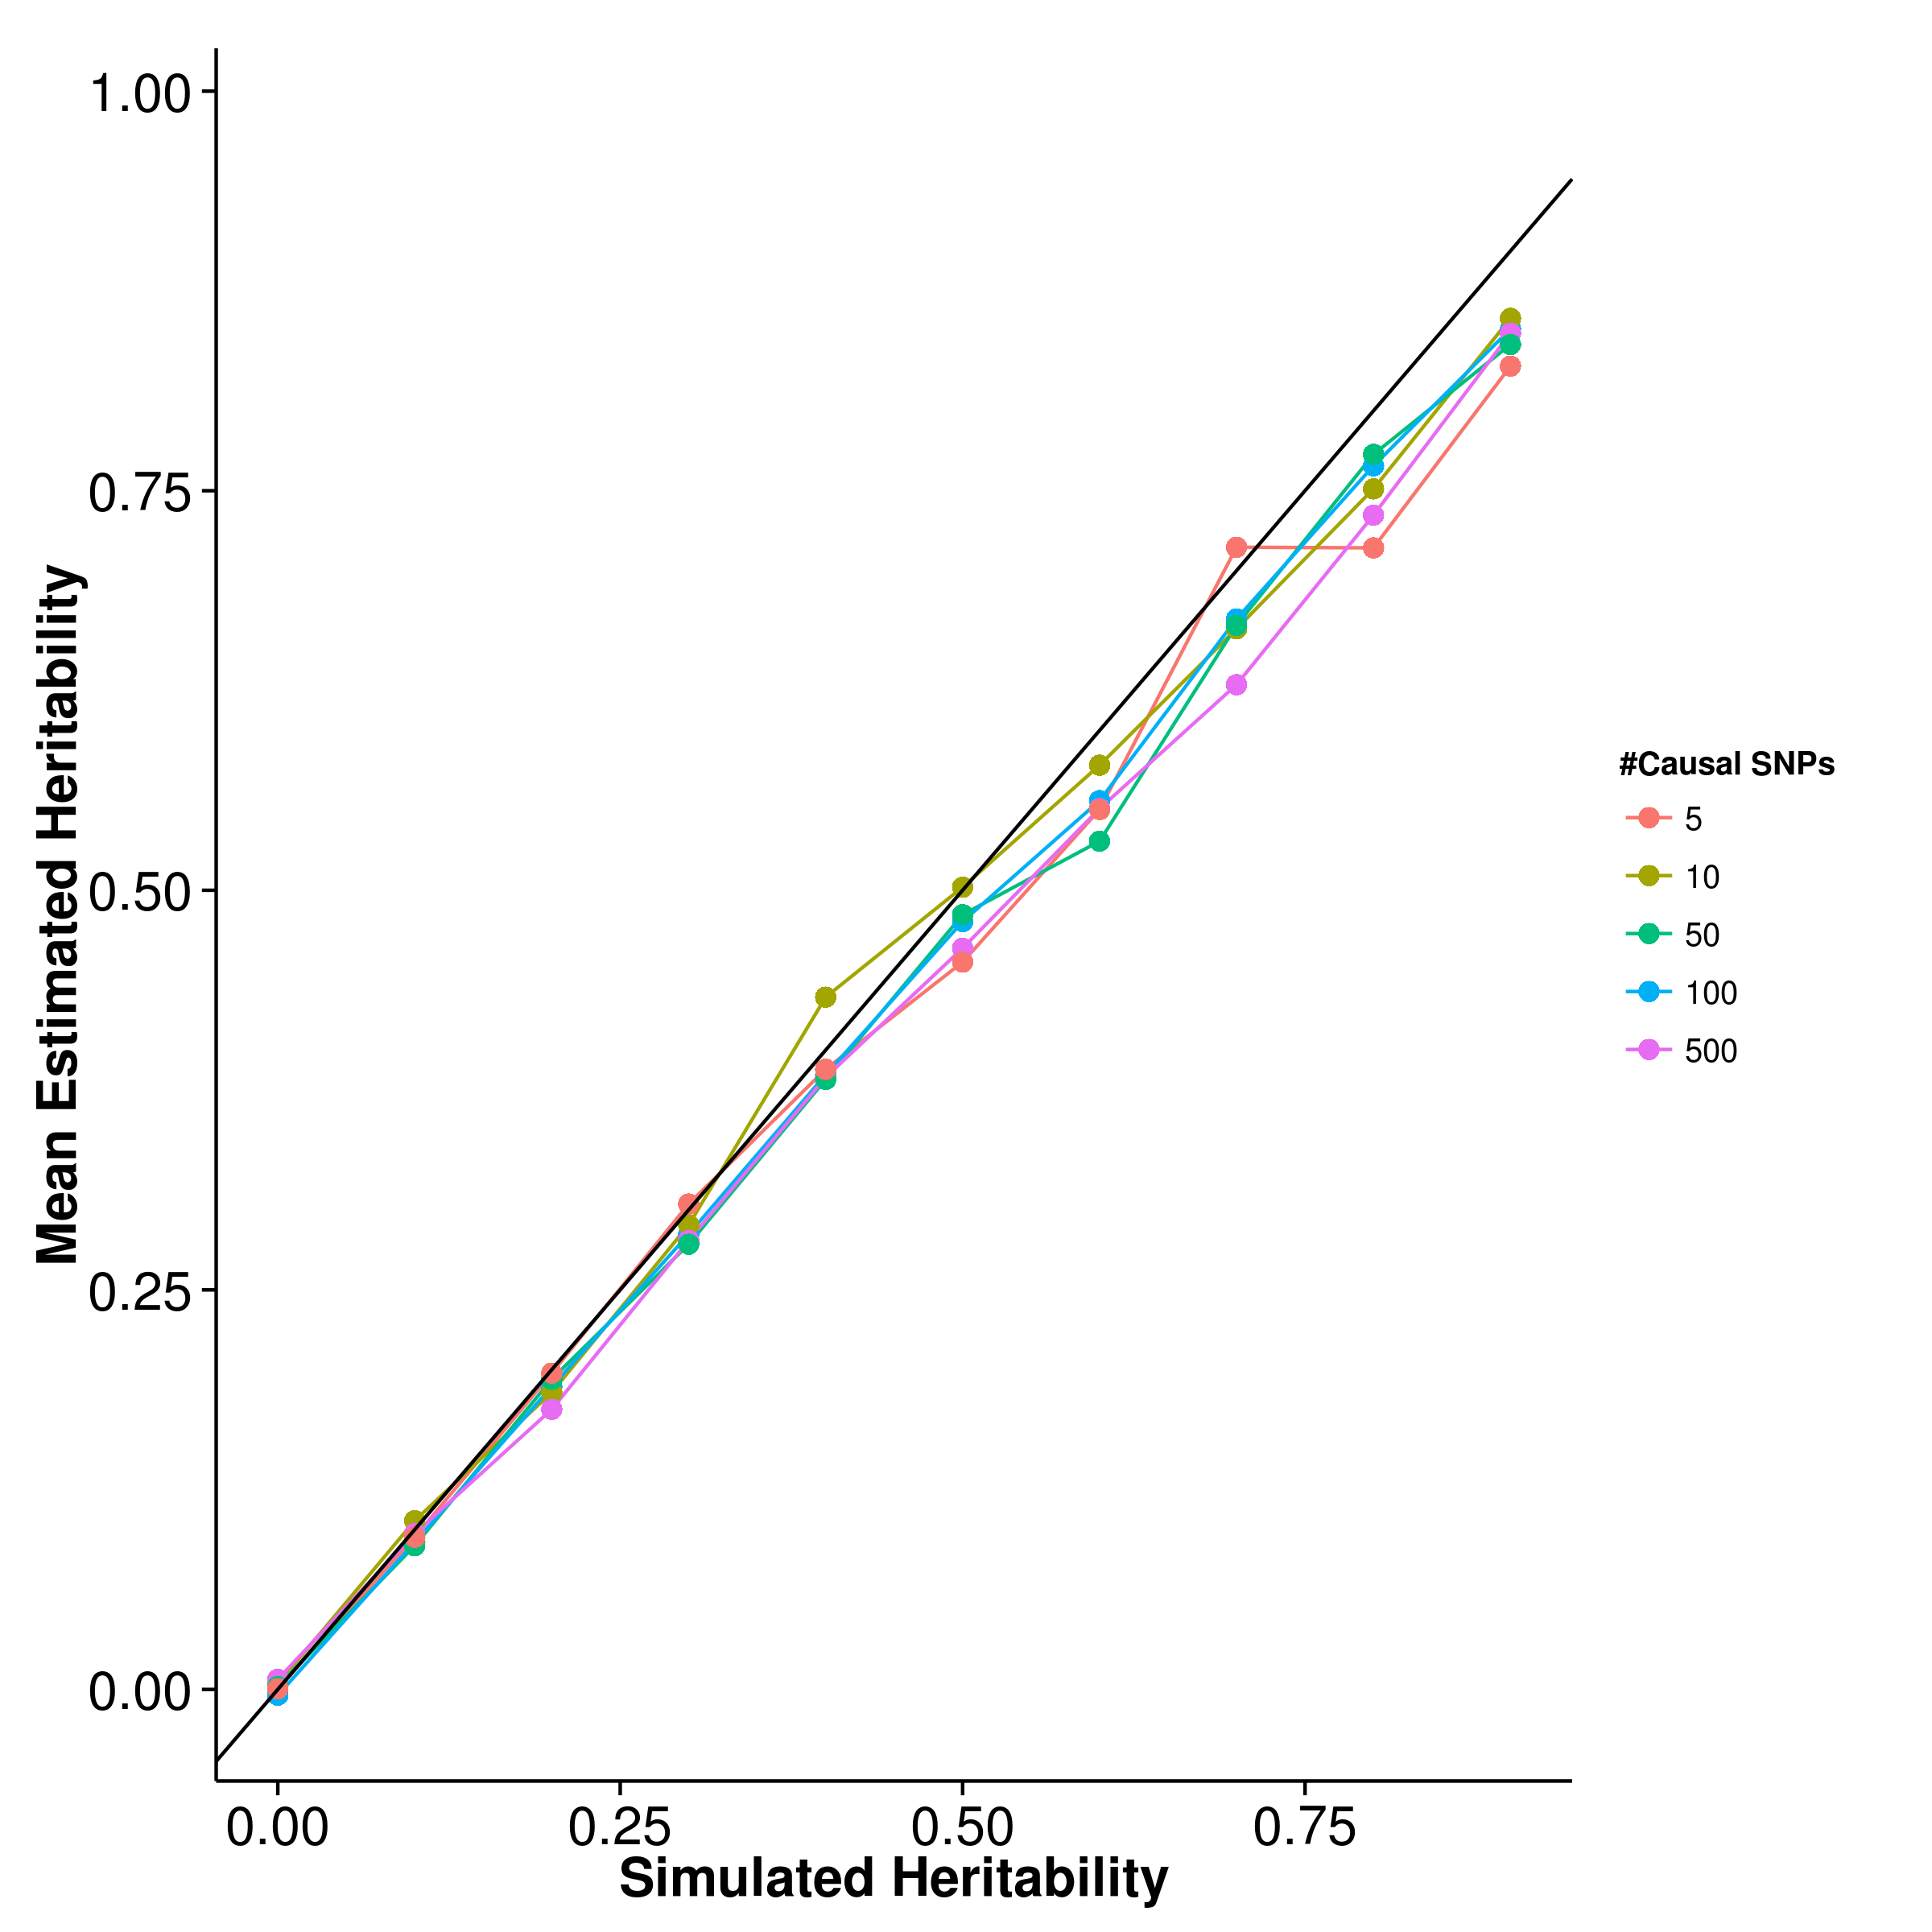
\includegraphics{figure/he_summary/random/gcta_Qt_Rand_mean.png}}
				\label{fig:gctaQtRandMean}
			}\\
			\subfloat[LDSC with fix intercept]{
				\scalebox{.4}{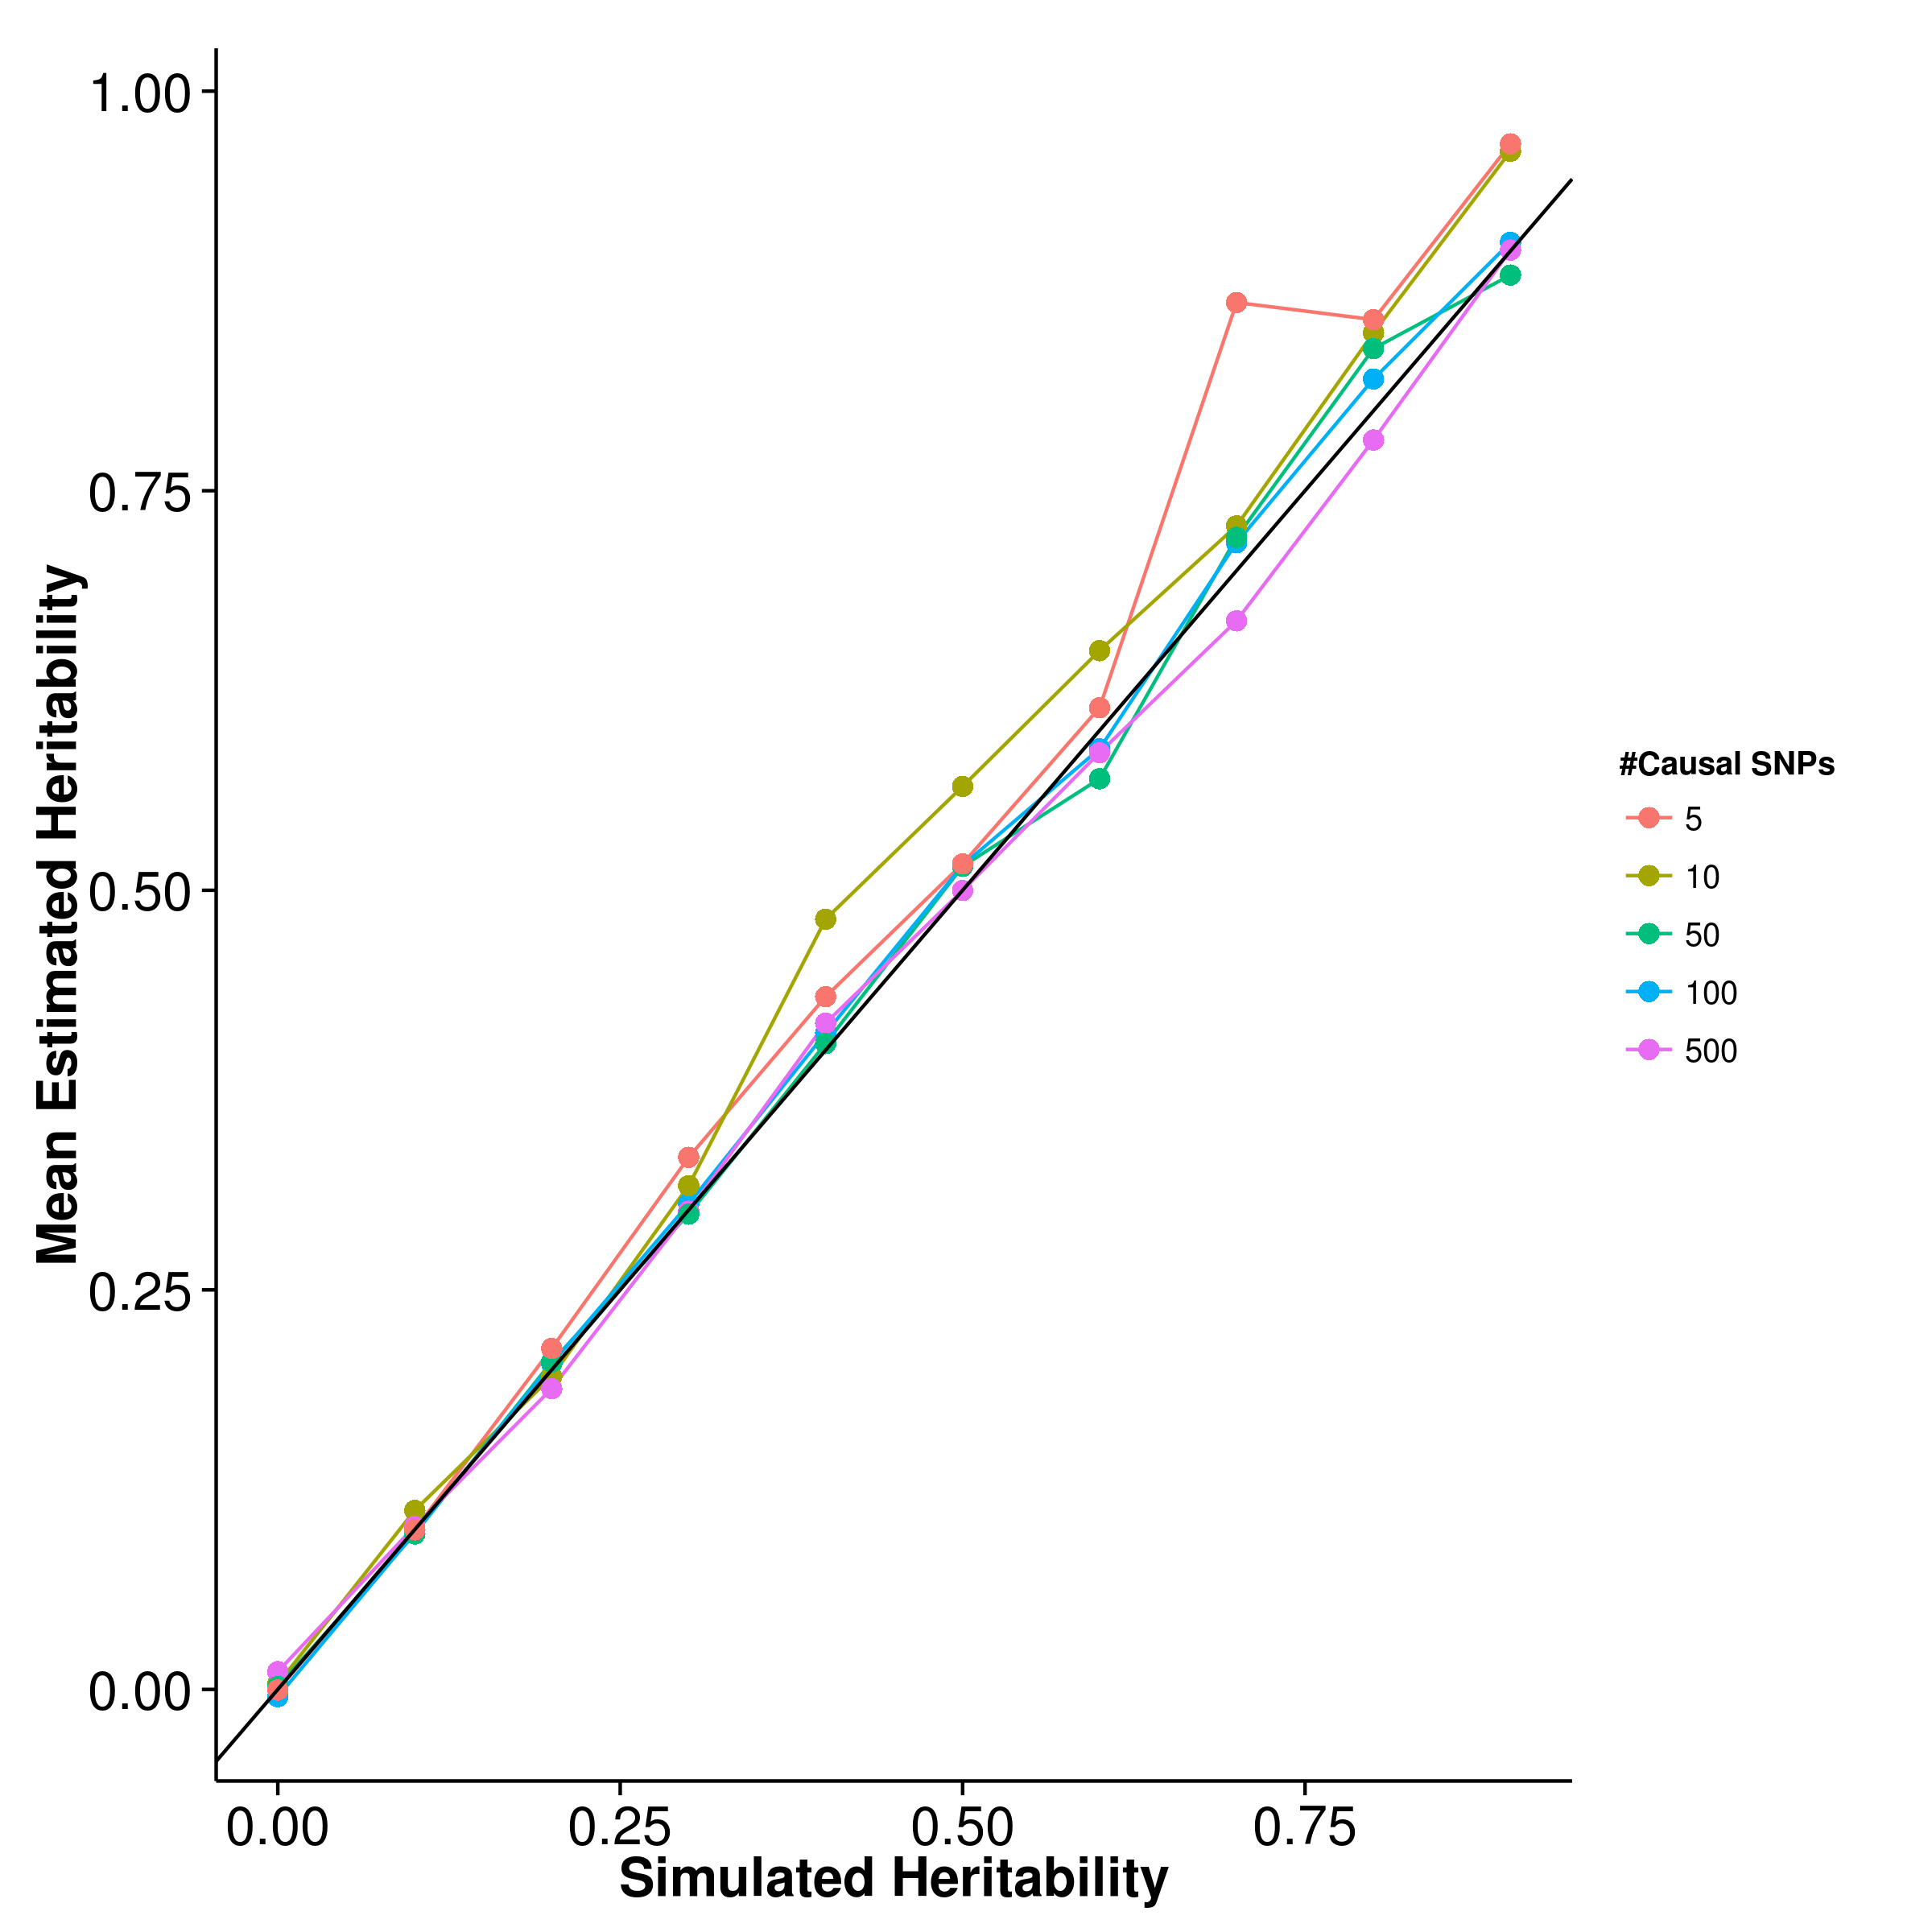
\includegraphics{figure/he_summary/random/ldsc_Qt_Rand_mean.png}}
				\label{fig:ldscQtRandMean}
			}
			\subfloat[LDSC with intercept estimation]{
				
				\scalebox{.4}{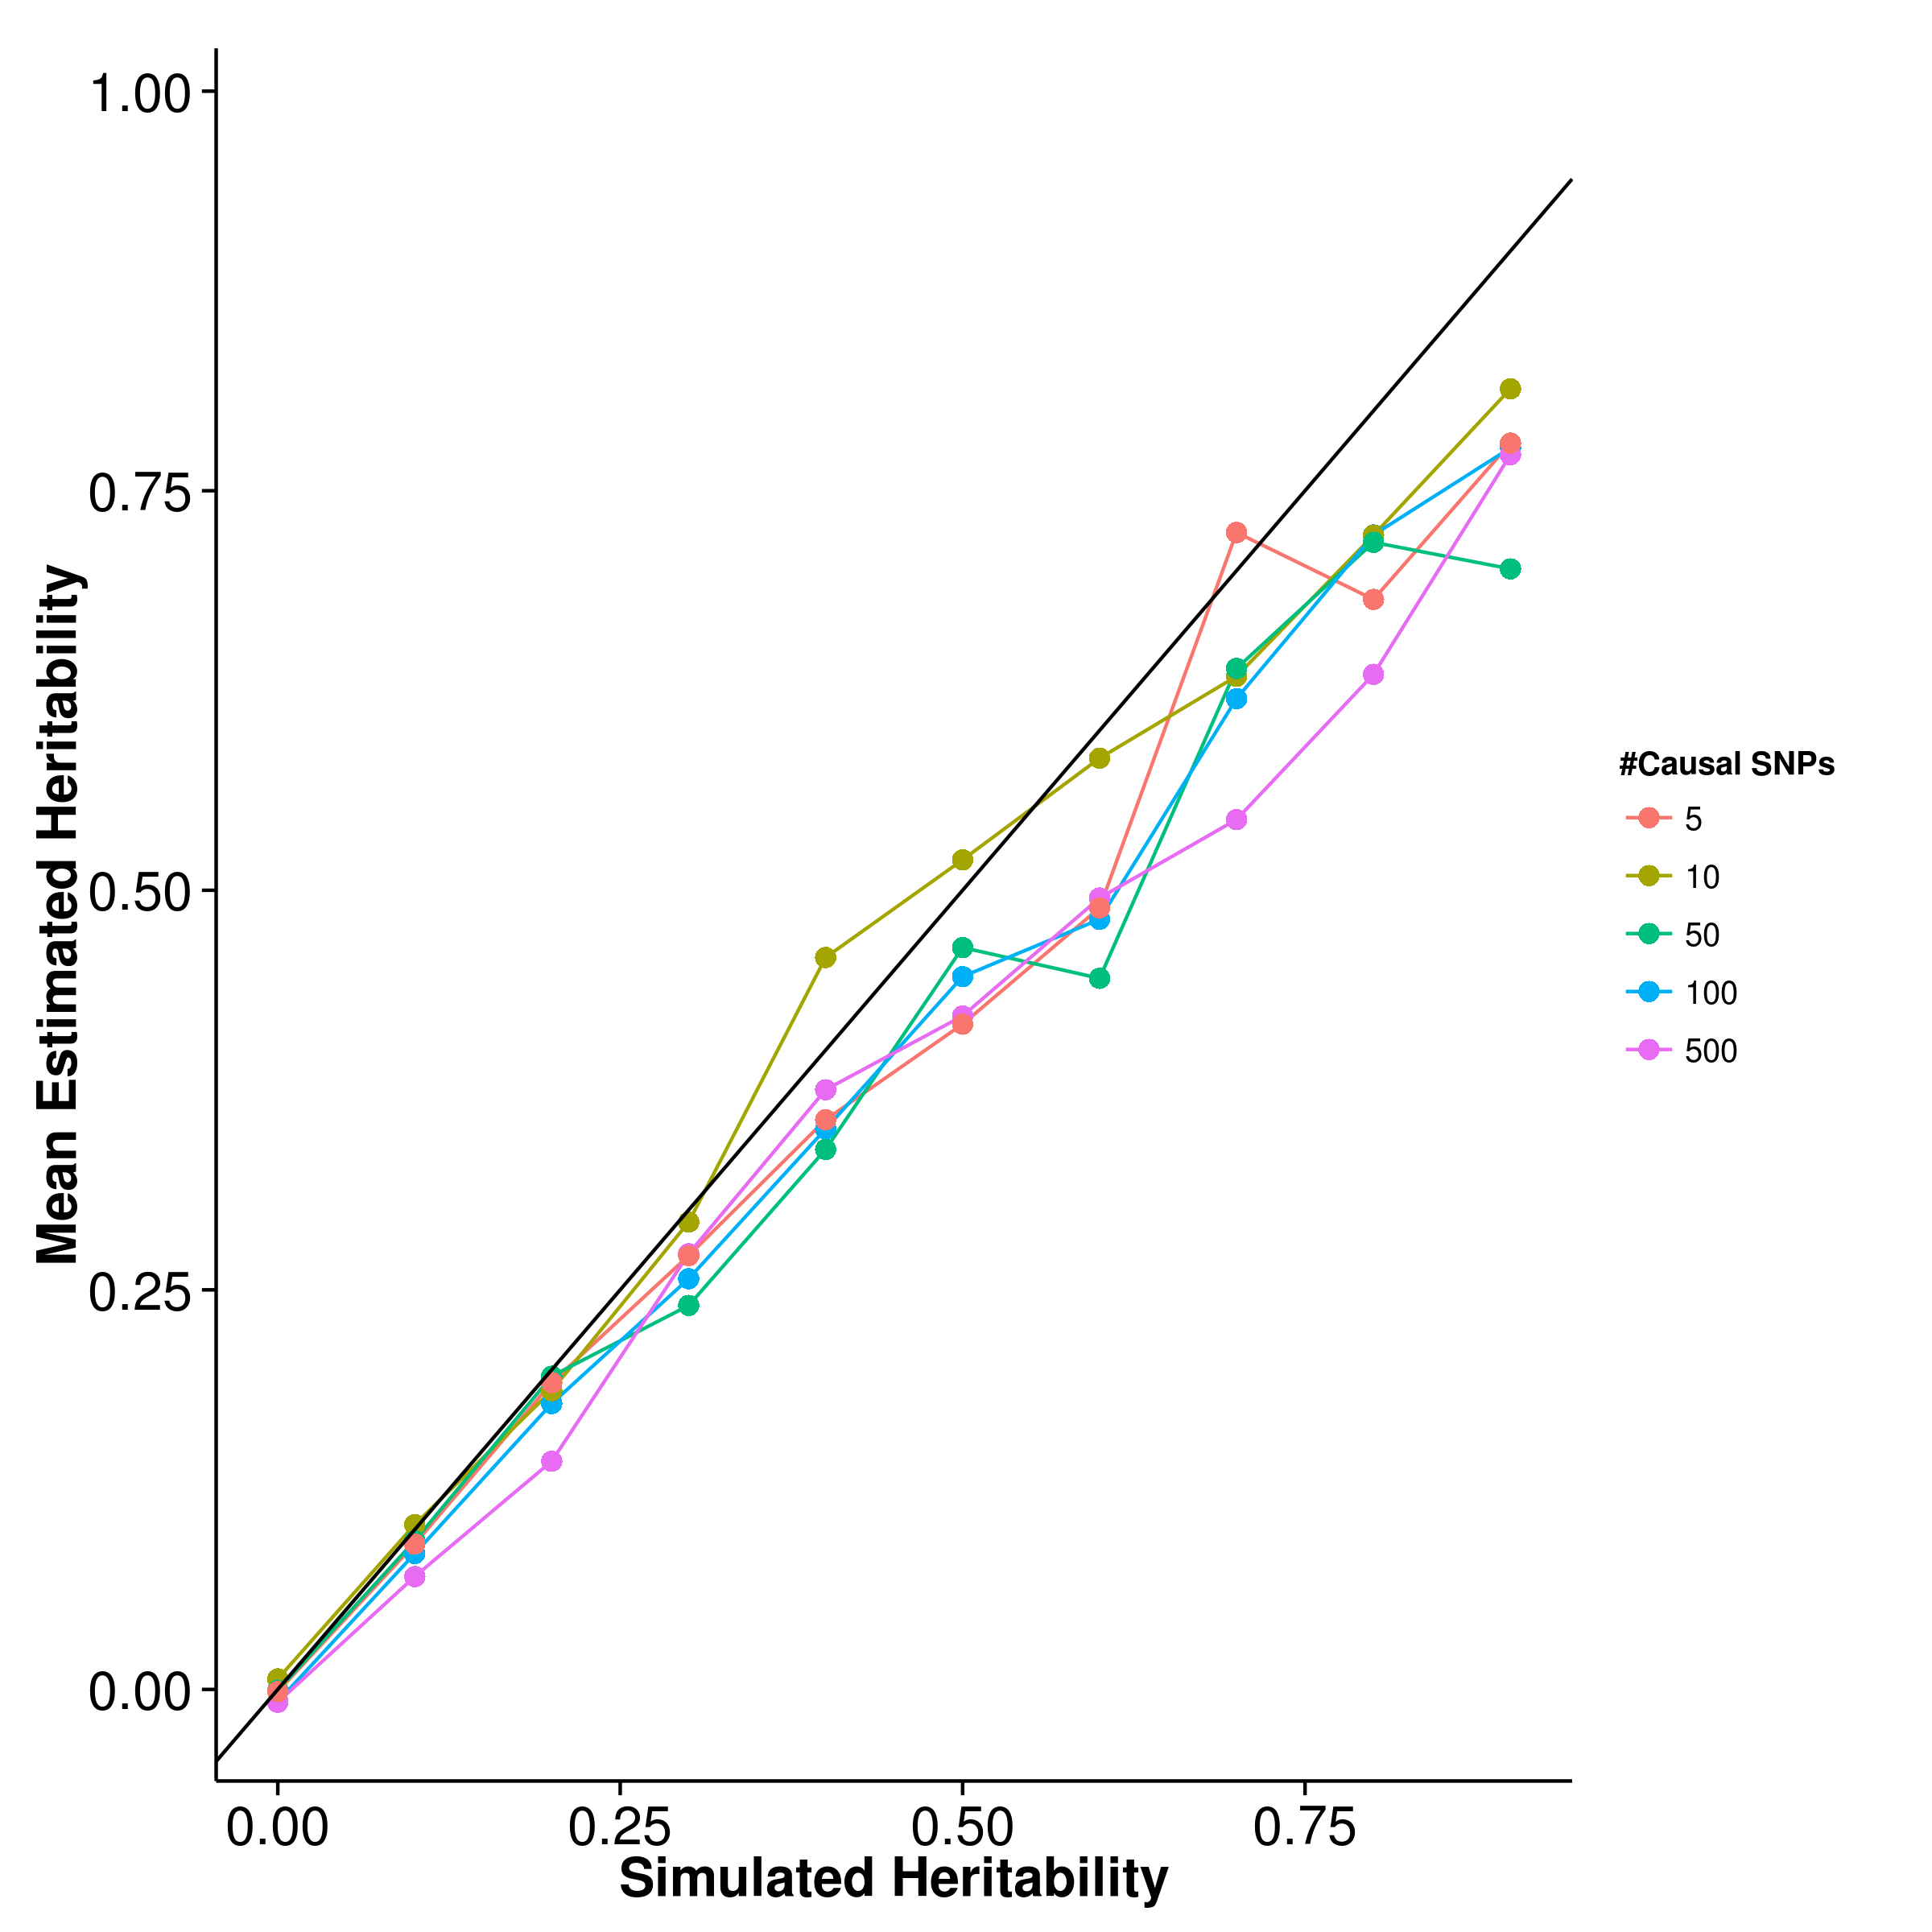
\includegraphics{figure/he_summary/random/ldscIn_Qt_Rand_mean.png}}
				\label{fig:ldscInQtRandMean}
			}
			\caption[Mean of Quantitative Trait Simulation Results]
			{Mean of results from quantitative trait simulation with random effect size simulation.
				Estimations form \gls{shrek} were slightly biased upwards whereas \gls{gcta} and \gls{ldsc} with intercept estimations both biased downwards.
				On the other hand, \gls{ldsc} with fixed intercept provides least biased estimates under polygenic conditions. 
				However, when the number of causal \glspl{SNP} is small (e.g. 5 or 10), an upward bias was observed.} 
			\label{fig:QtRandMean}
		\end{figure}
		
		\begin{figure}
			\centering
			\subfloat[SHREK]{
				\scalebox{.4}{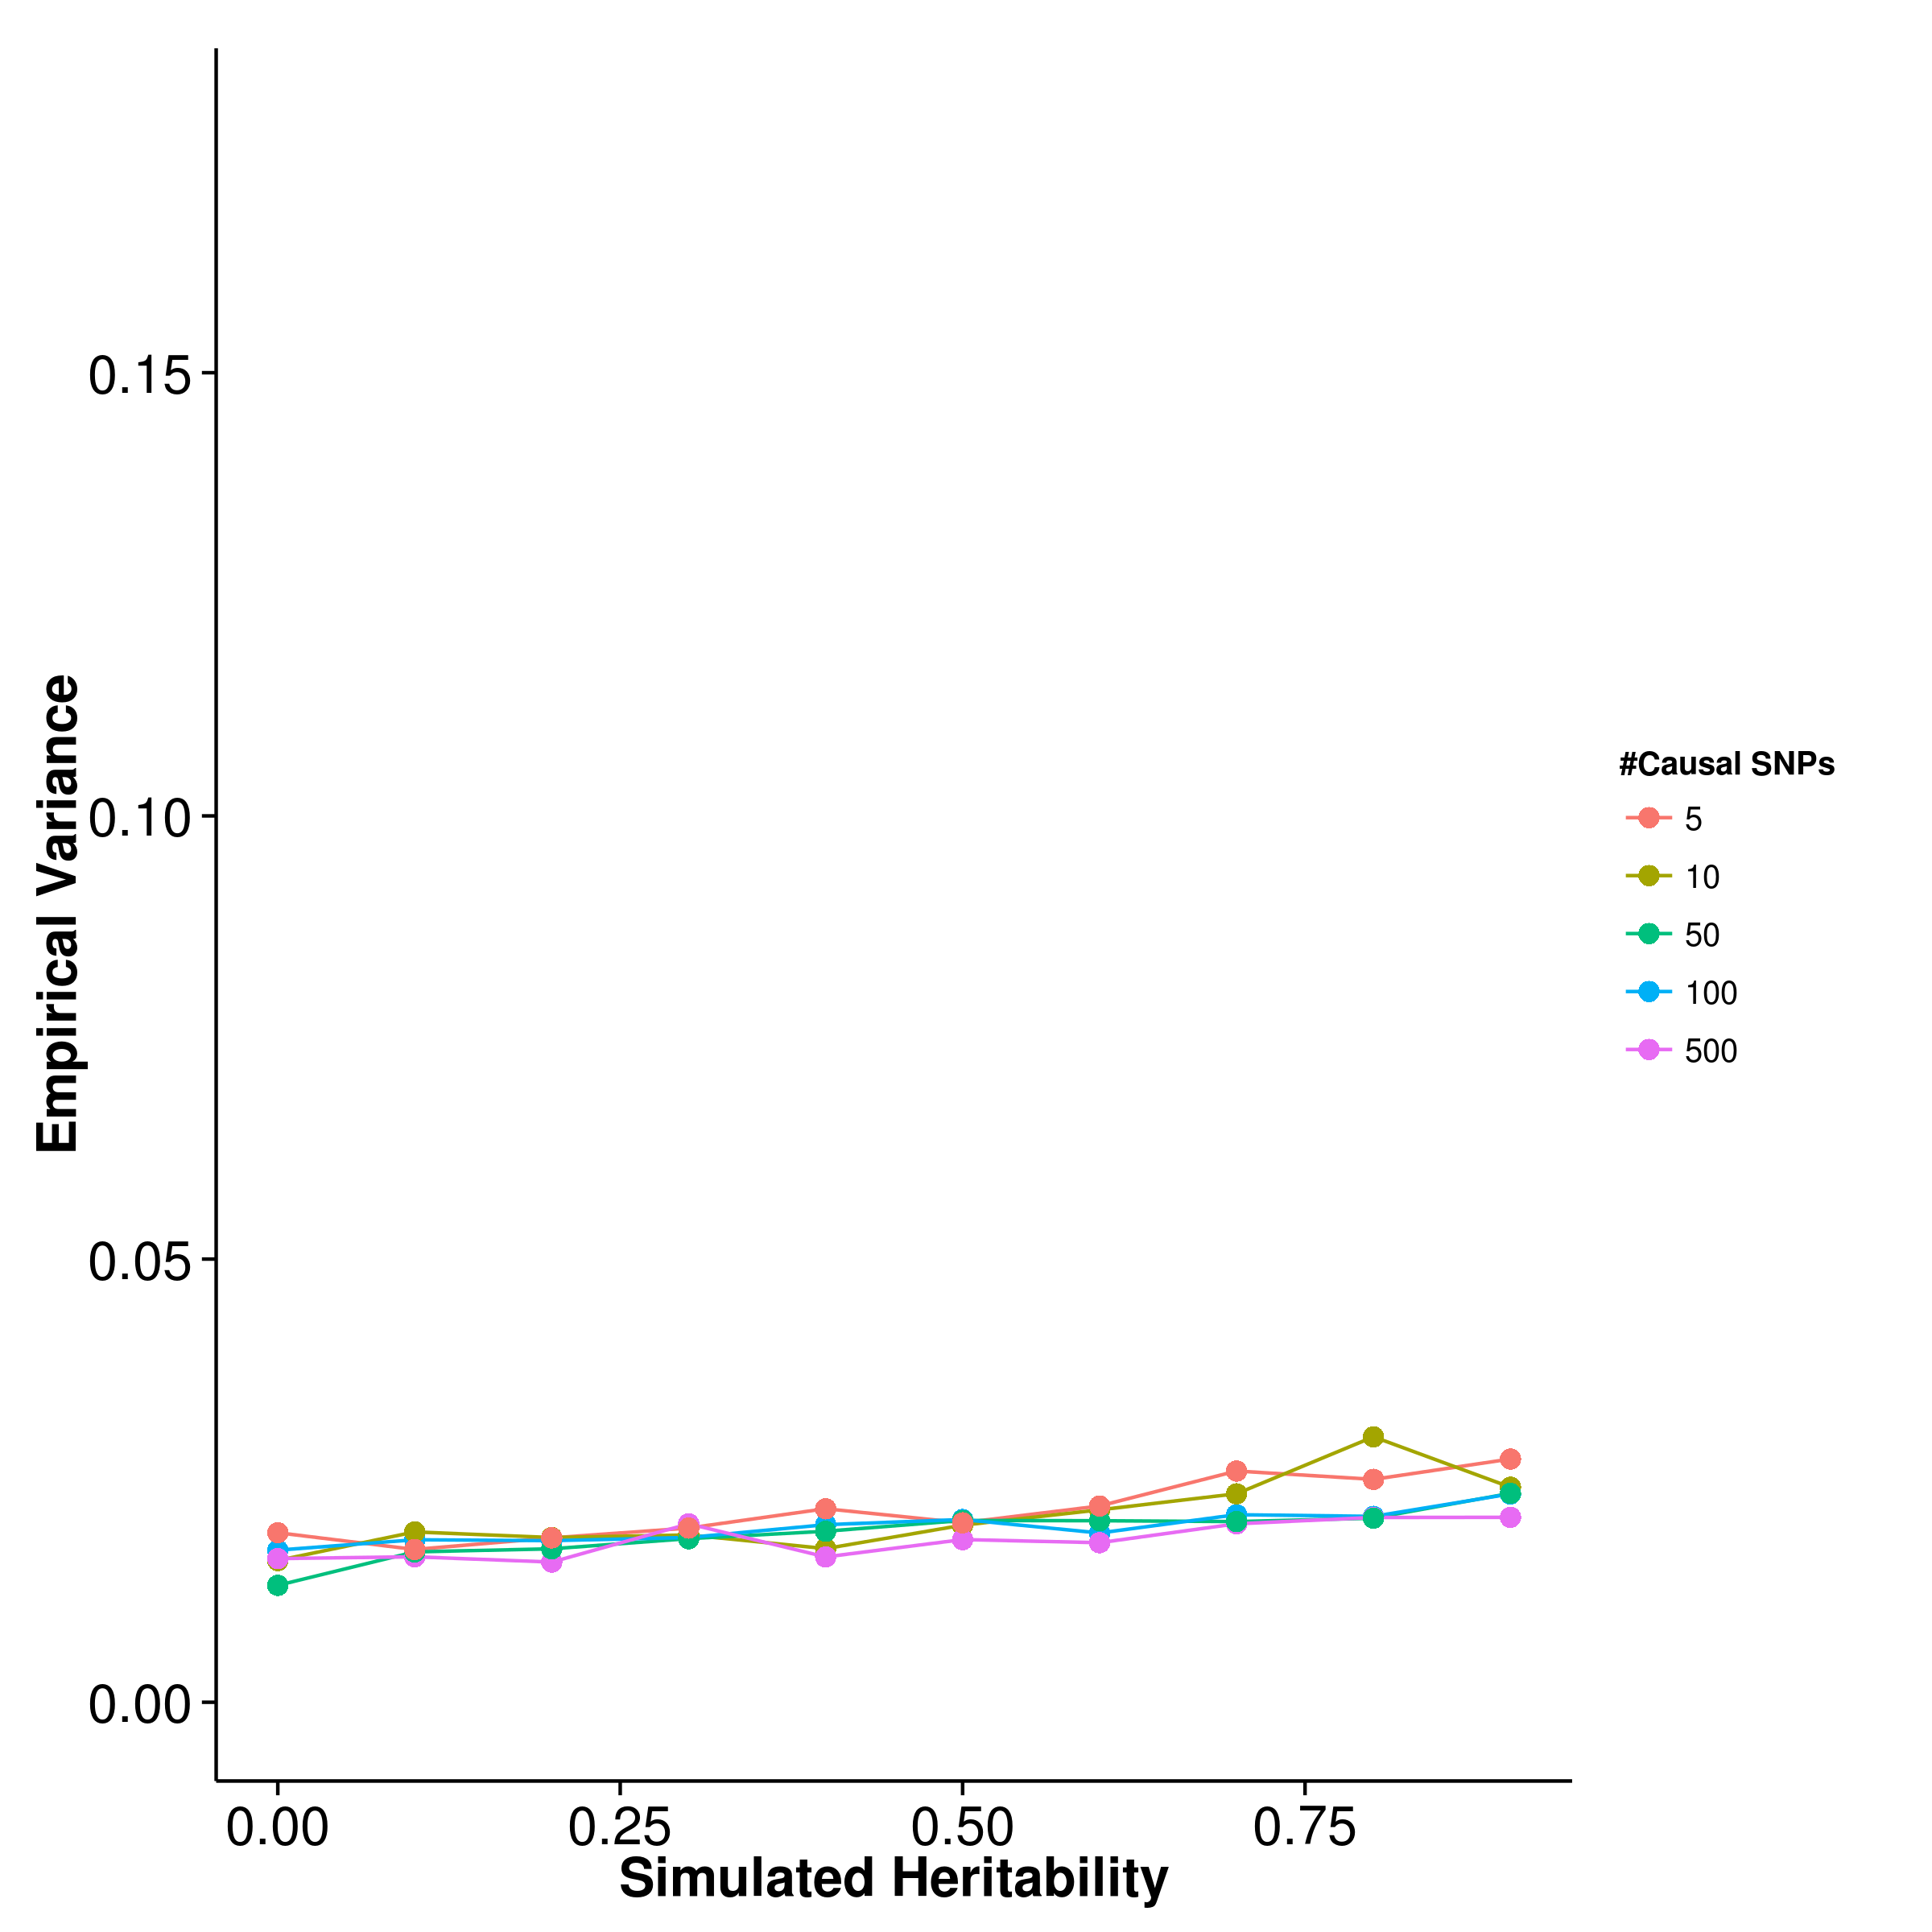
\includegraphics{figure/he_summary/random/shrek_Qt_Rand_sd.png}}
				\label{fig:shrekQtRandVar}
			}
			\subfloat[GCTA]{
				\scalebox{.4}{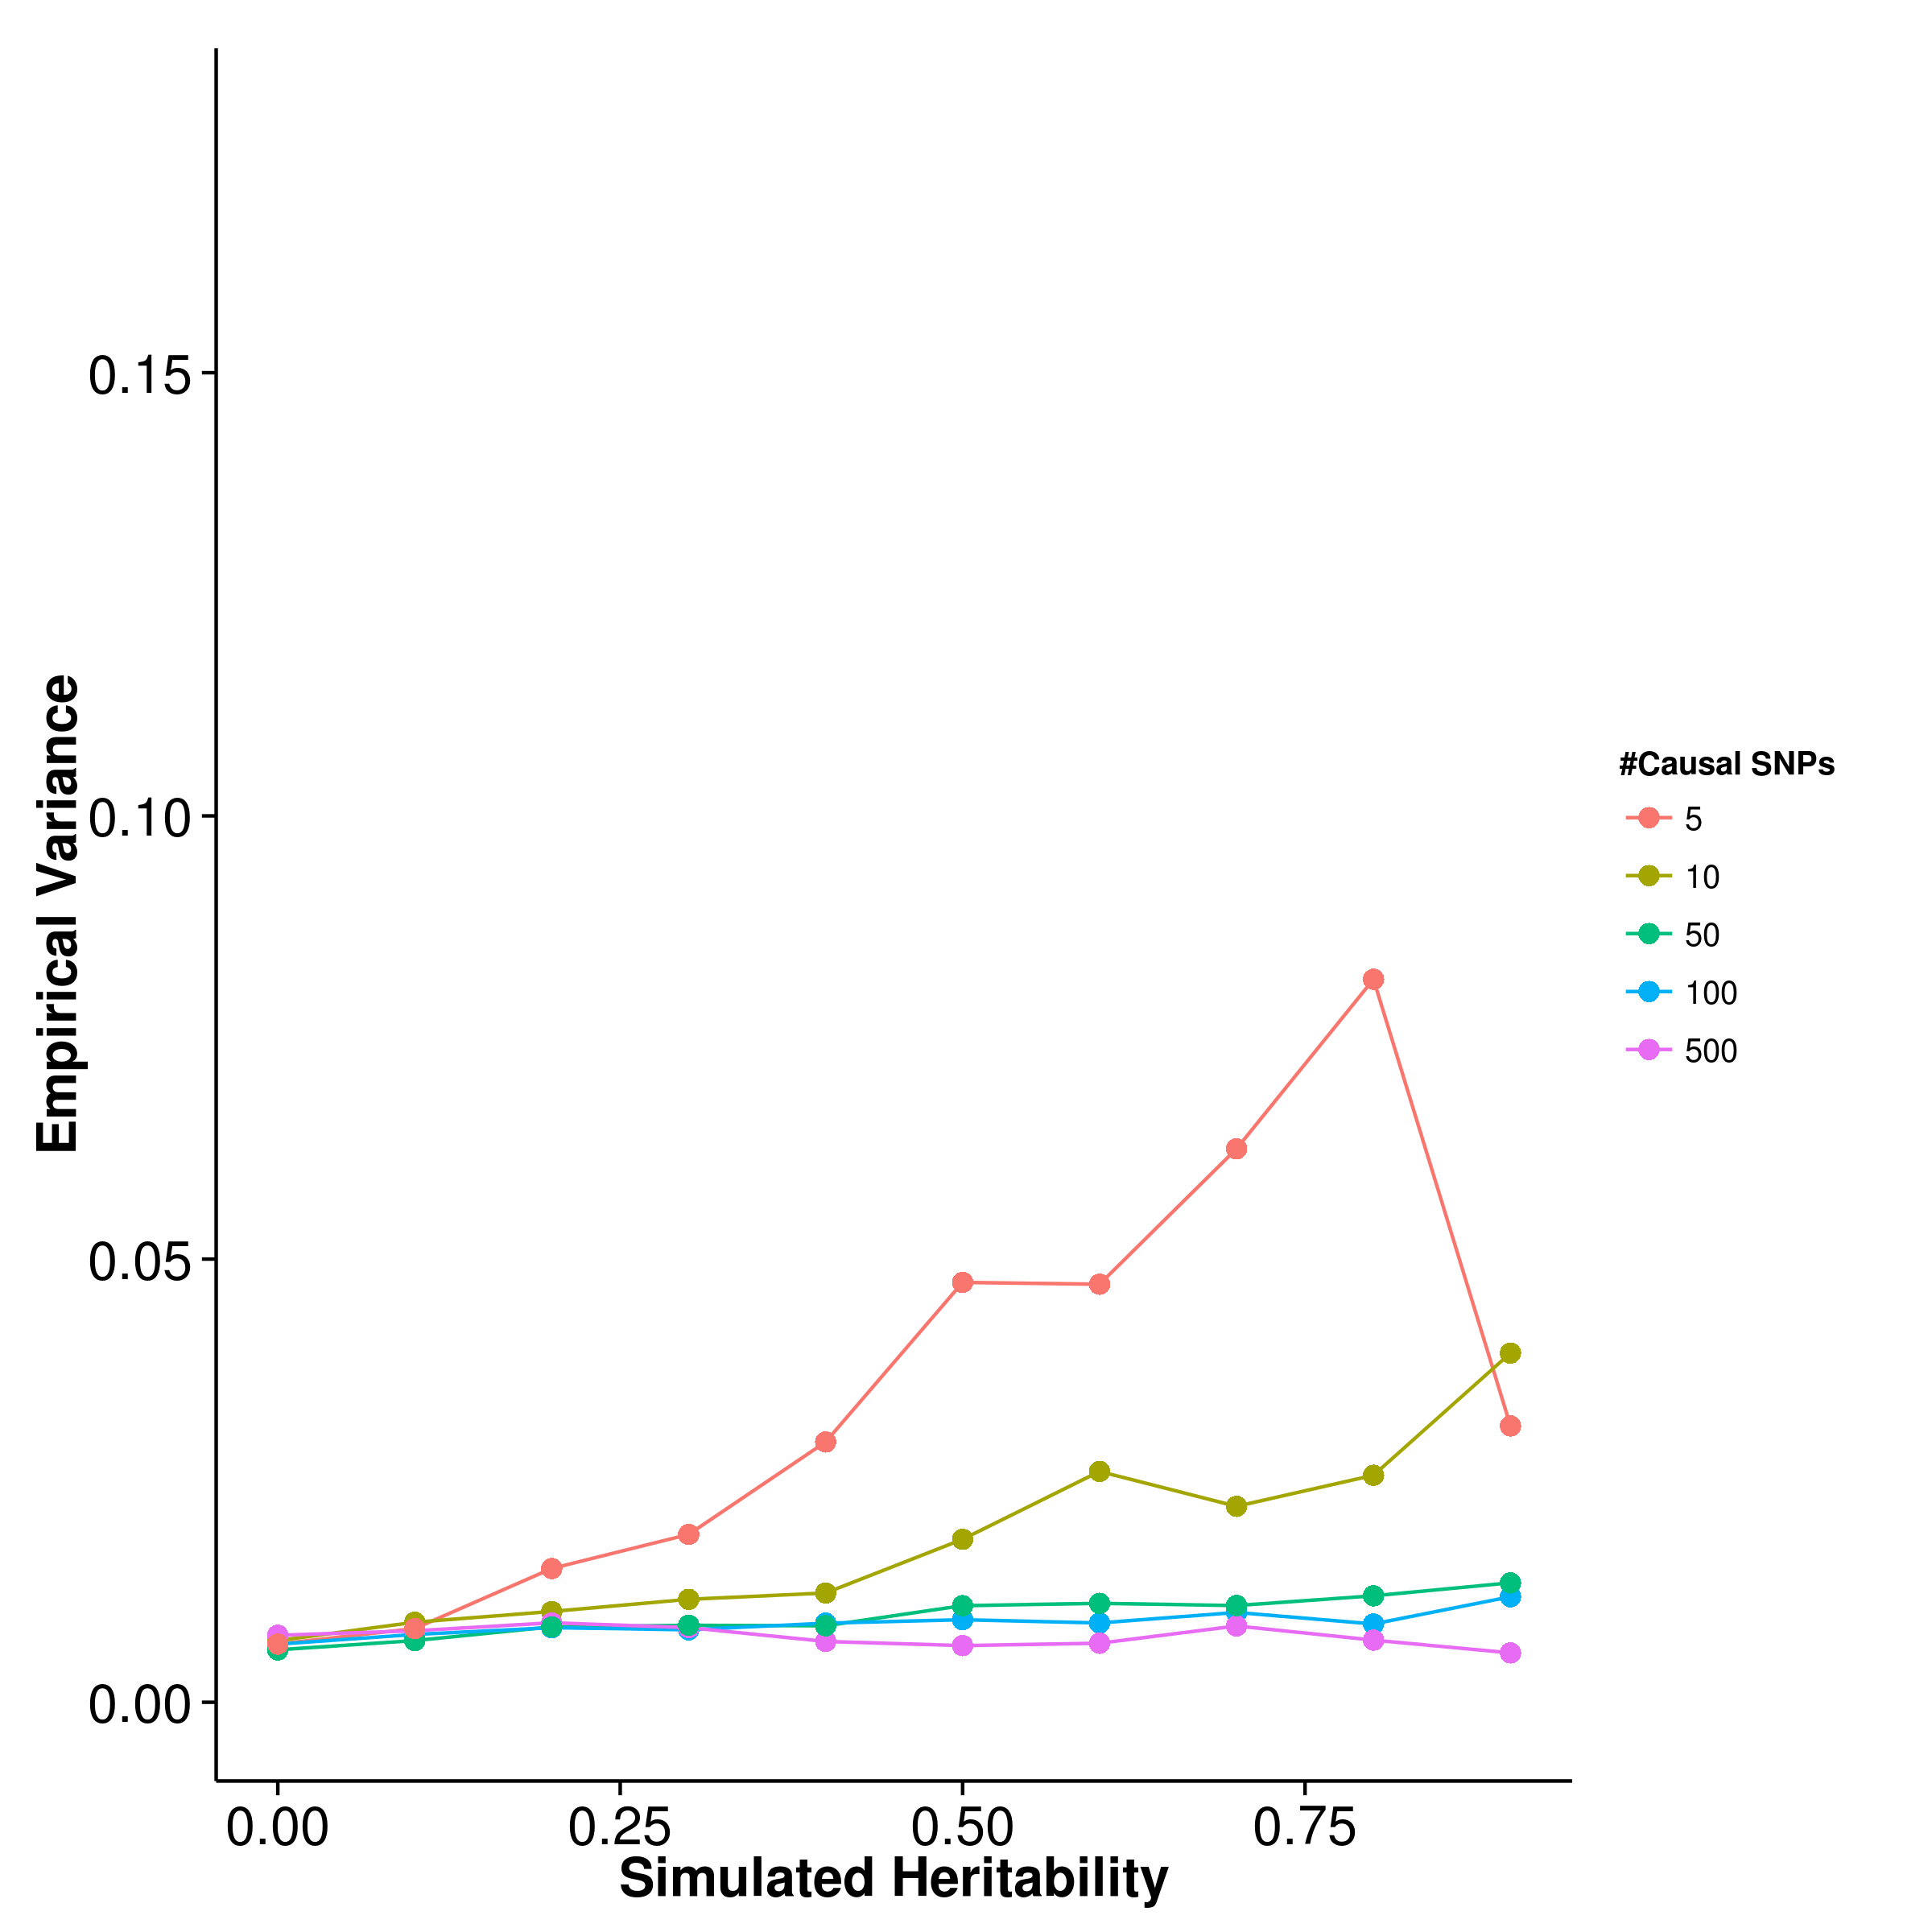
\includegraphics{figure/he_summary/random/gcta_Qt_Rand_sd.png}}
				\label{fig:gctaQtRandVar}
			}\\
			\subfloat[LDSC with fix intercept]{
				\scalebox{.4}{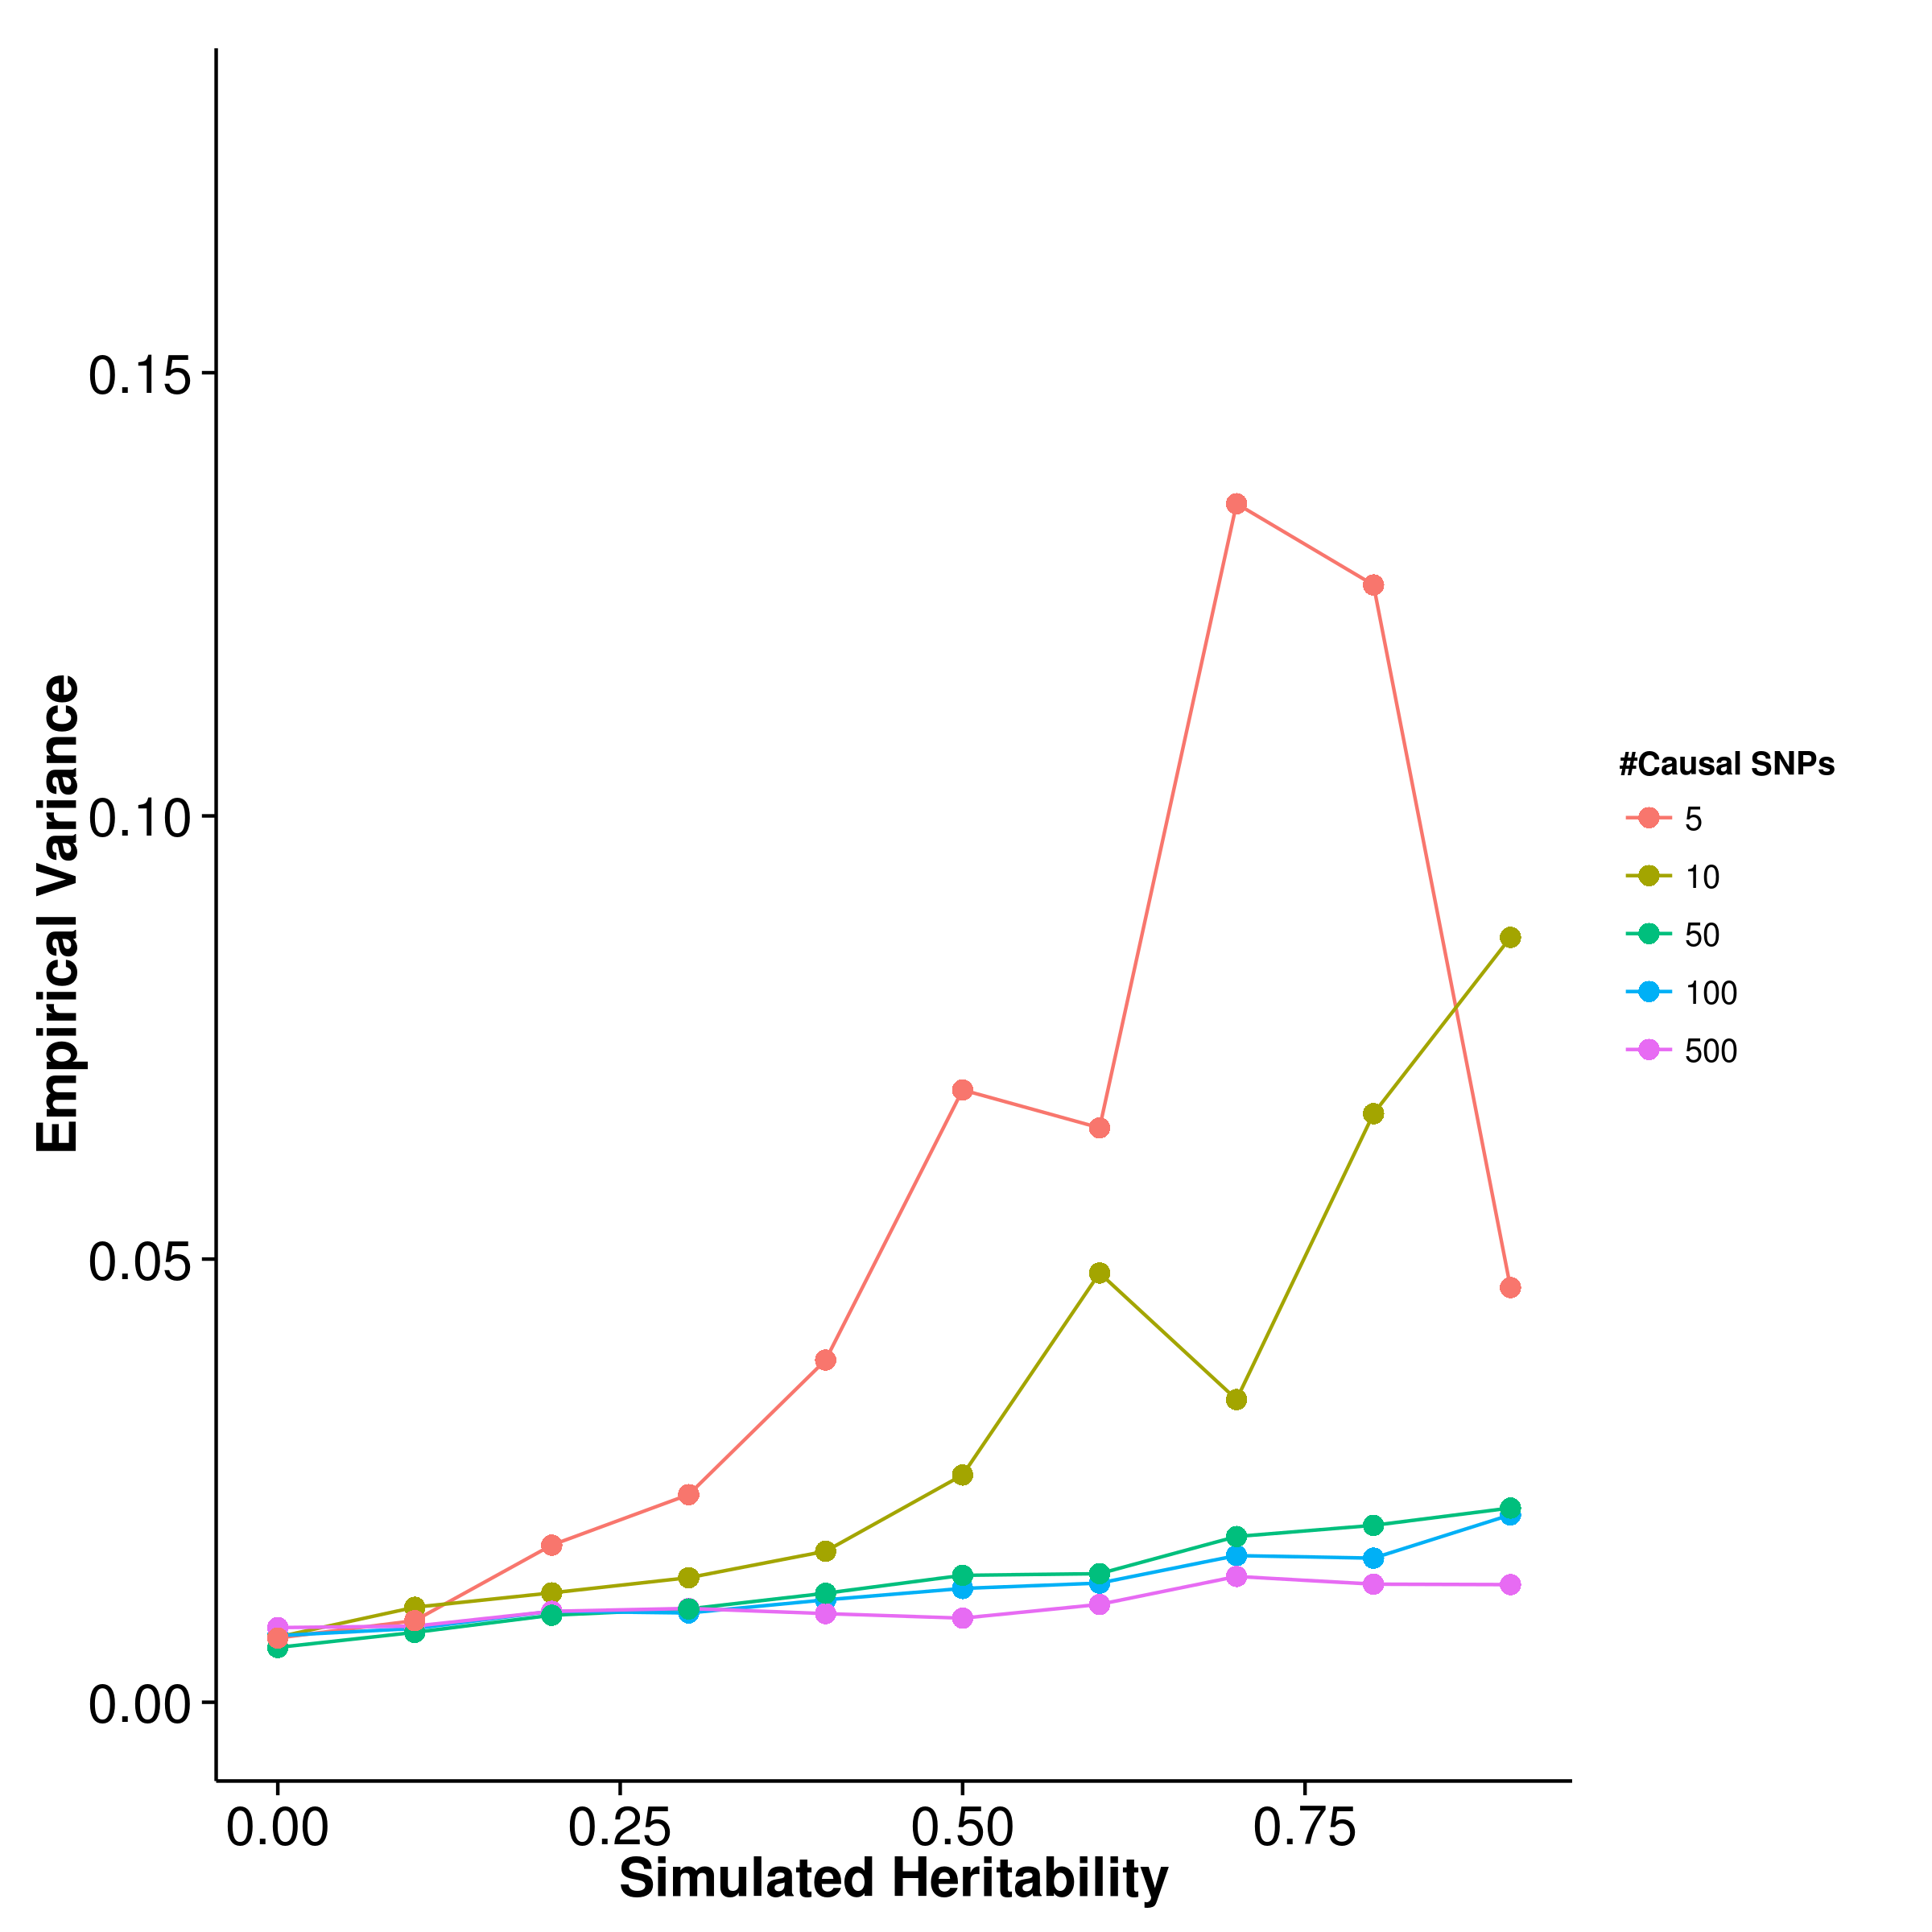
\includegraphics{figure/he_summary/random/ldsc_Qt_Rand_sd.png}}
				\label{fig:ldscQtRandVar}
			}
			\subfloat[LDSC with intercept estimation]{
				
				\scalebox{.4}{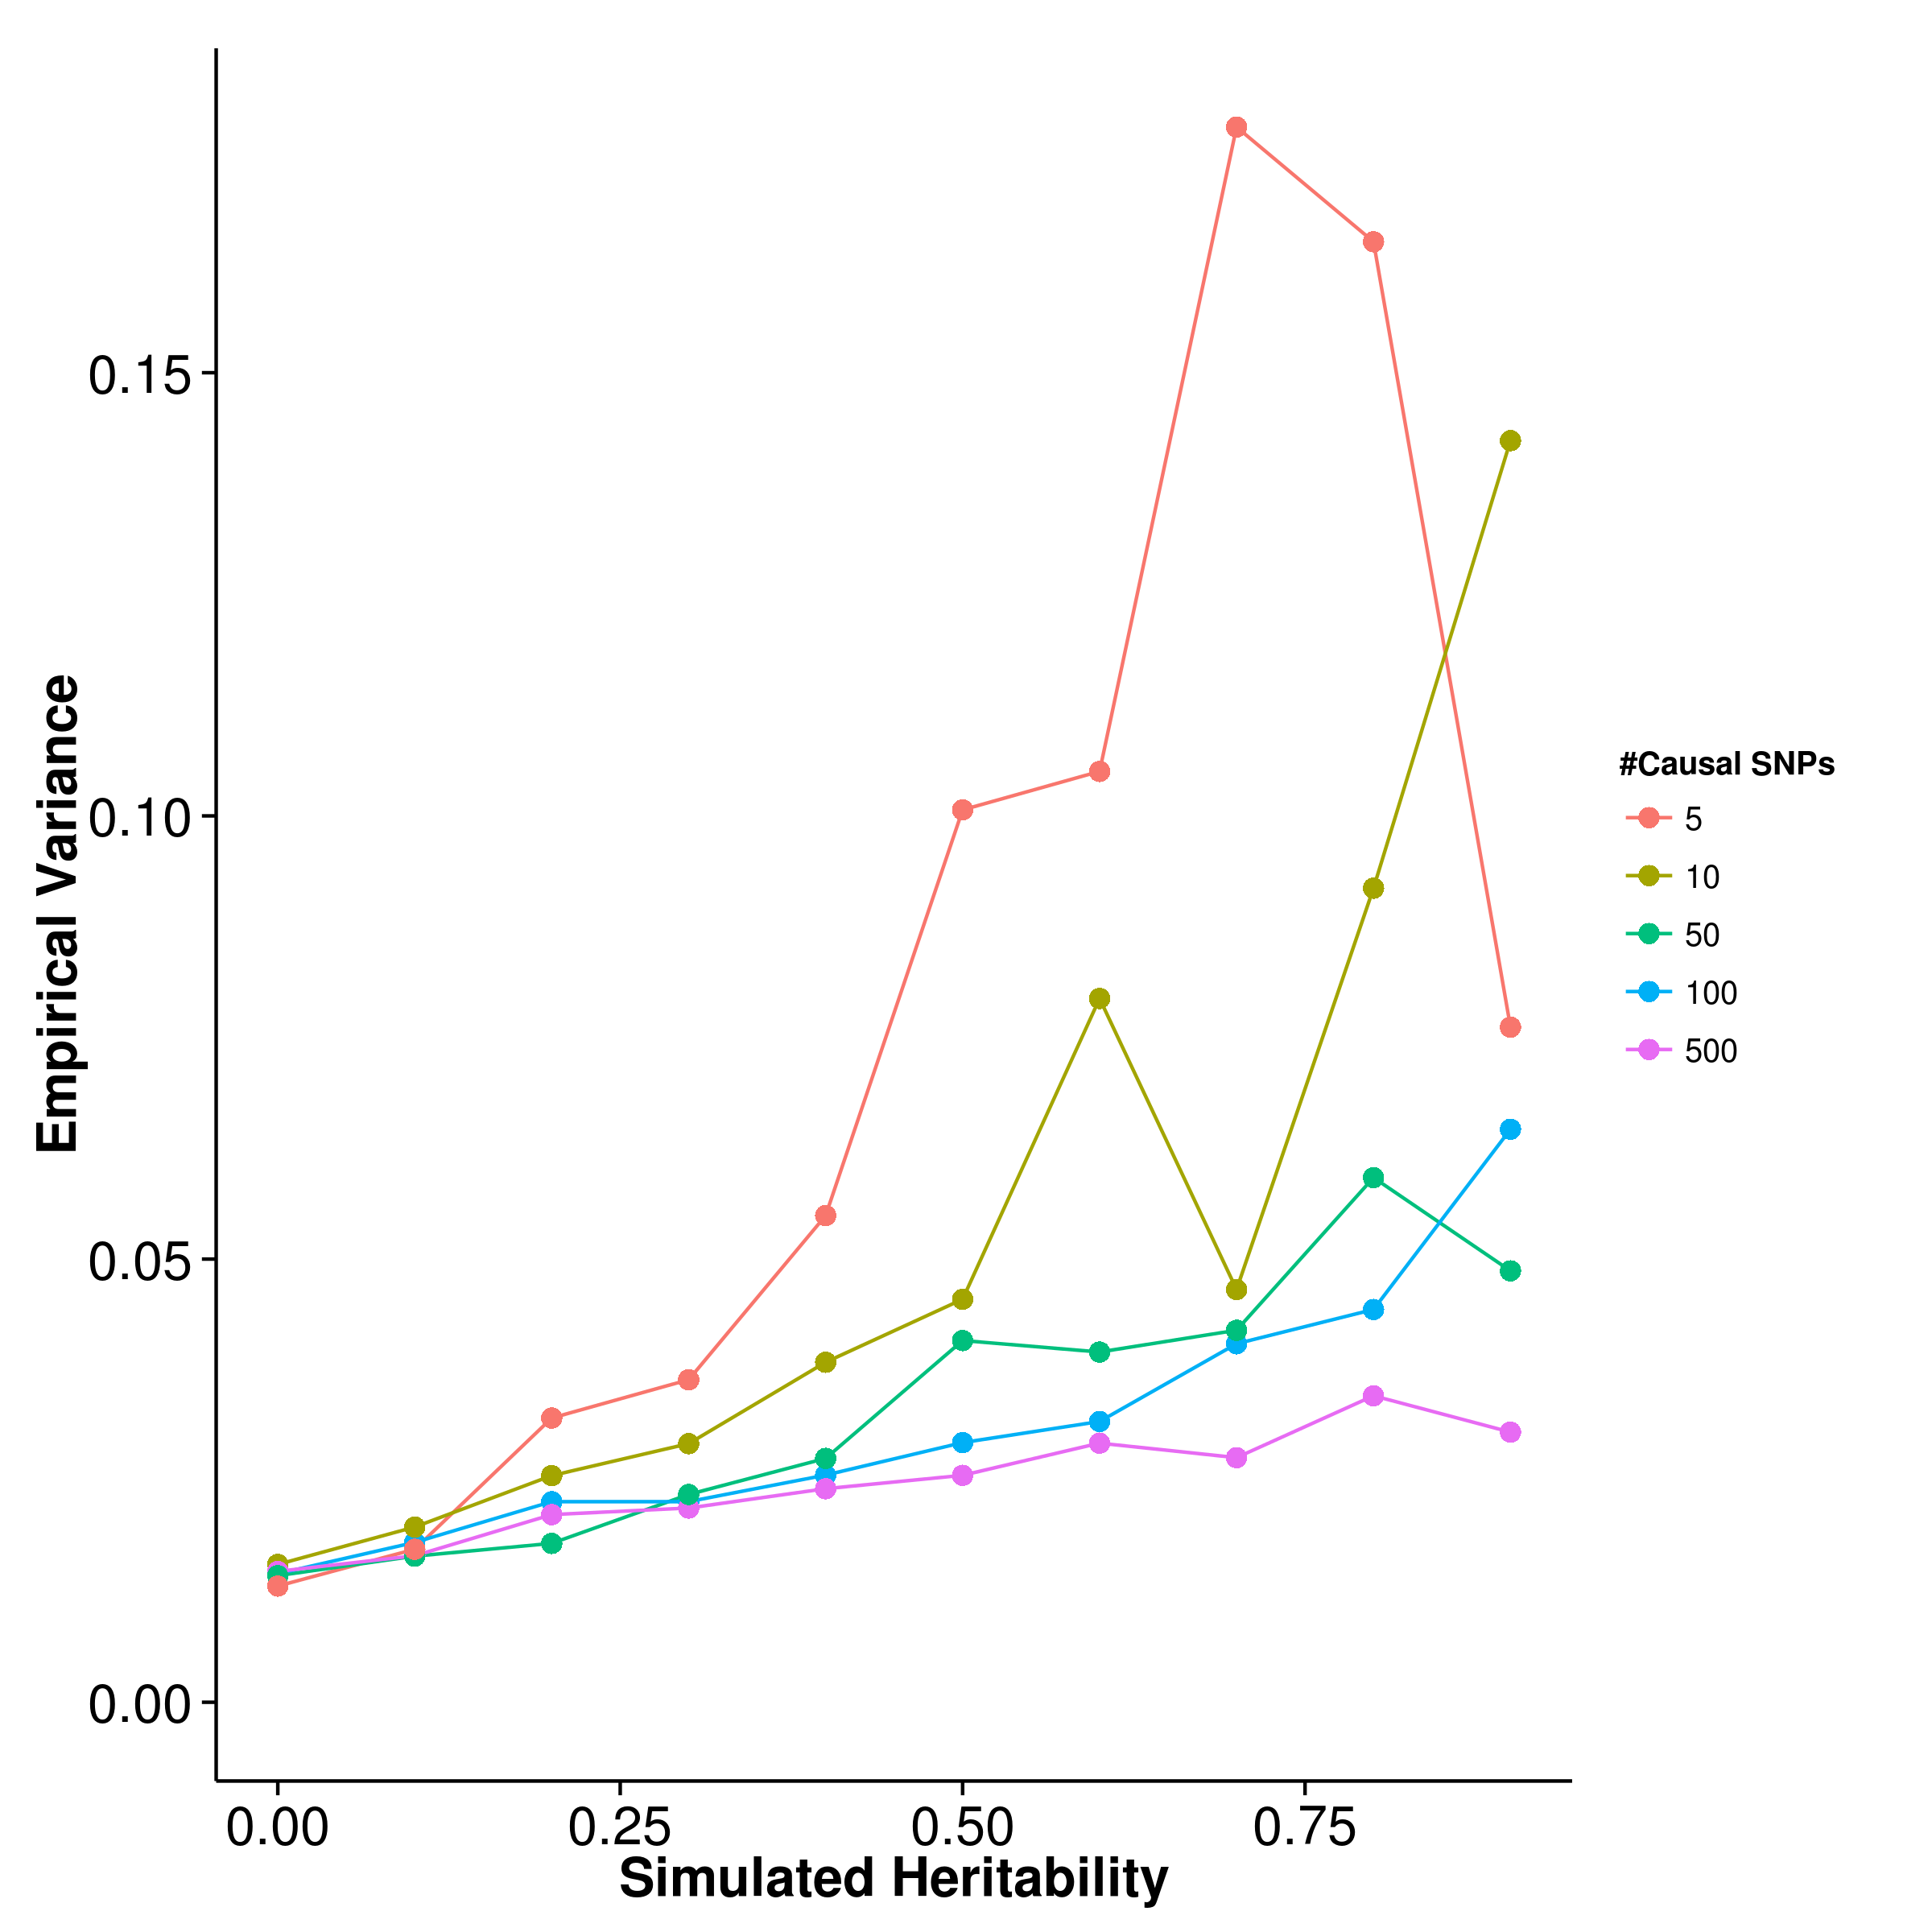
\includegraphics{figure/he_summary/random/ldscIn_Qt_Rand_sd.png}}
				\label{fig:ldscInQtRandVar}
			}
			\caption[Variance of Quantitative Trait Simulation Results]
			{Variance of results from quantitative trait simulation with random effect size simulation.
				Under the polygenic conditions, \gls{gcta} has the smallest variance, follow by \gls{ldsc}. 
				However, it was observed when the number of causal \glspl{SNP} decreases, the variance of the estimation increases for all algorithm, with variance of the \gls{shrek} estimate being the least affected.
				In fact, under oligogenic conditions, \gls{shrek} has a lower empirical variance when compared to \gls{ldsc}.
			} 
			\label{fig:QtRandVar}
		\end{figure}
		
		\begin{figure}
			\centering
			\subfloat[SHREK]{
				\scalebox{.4}{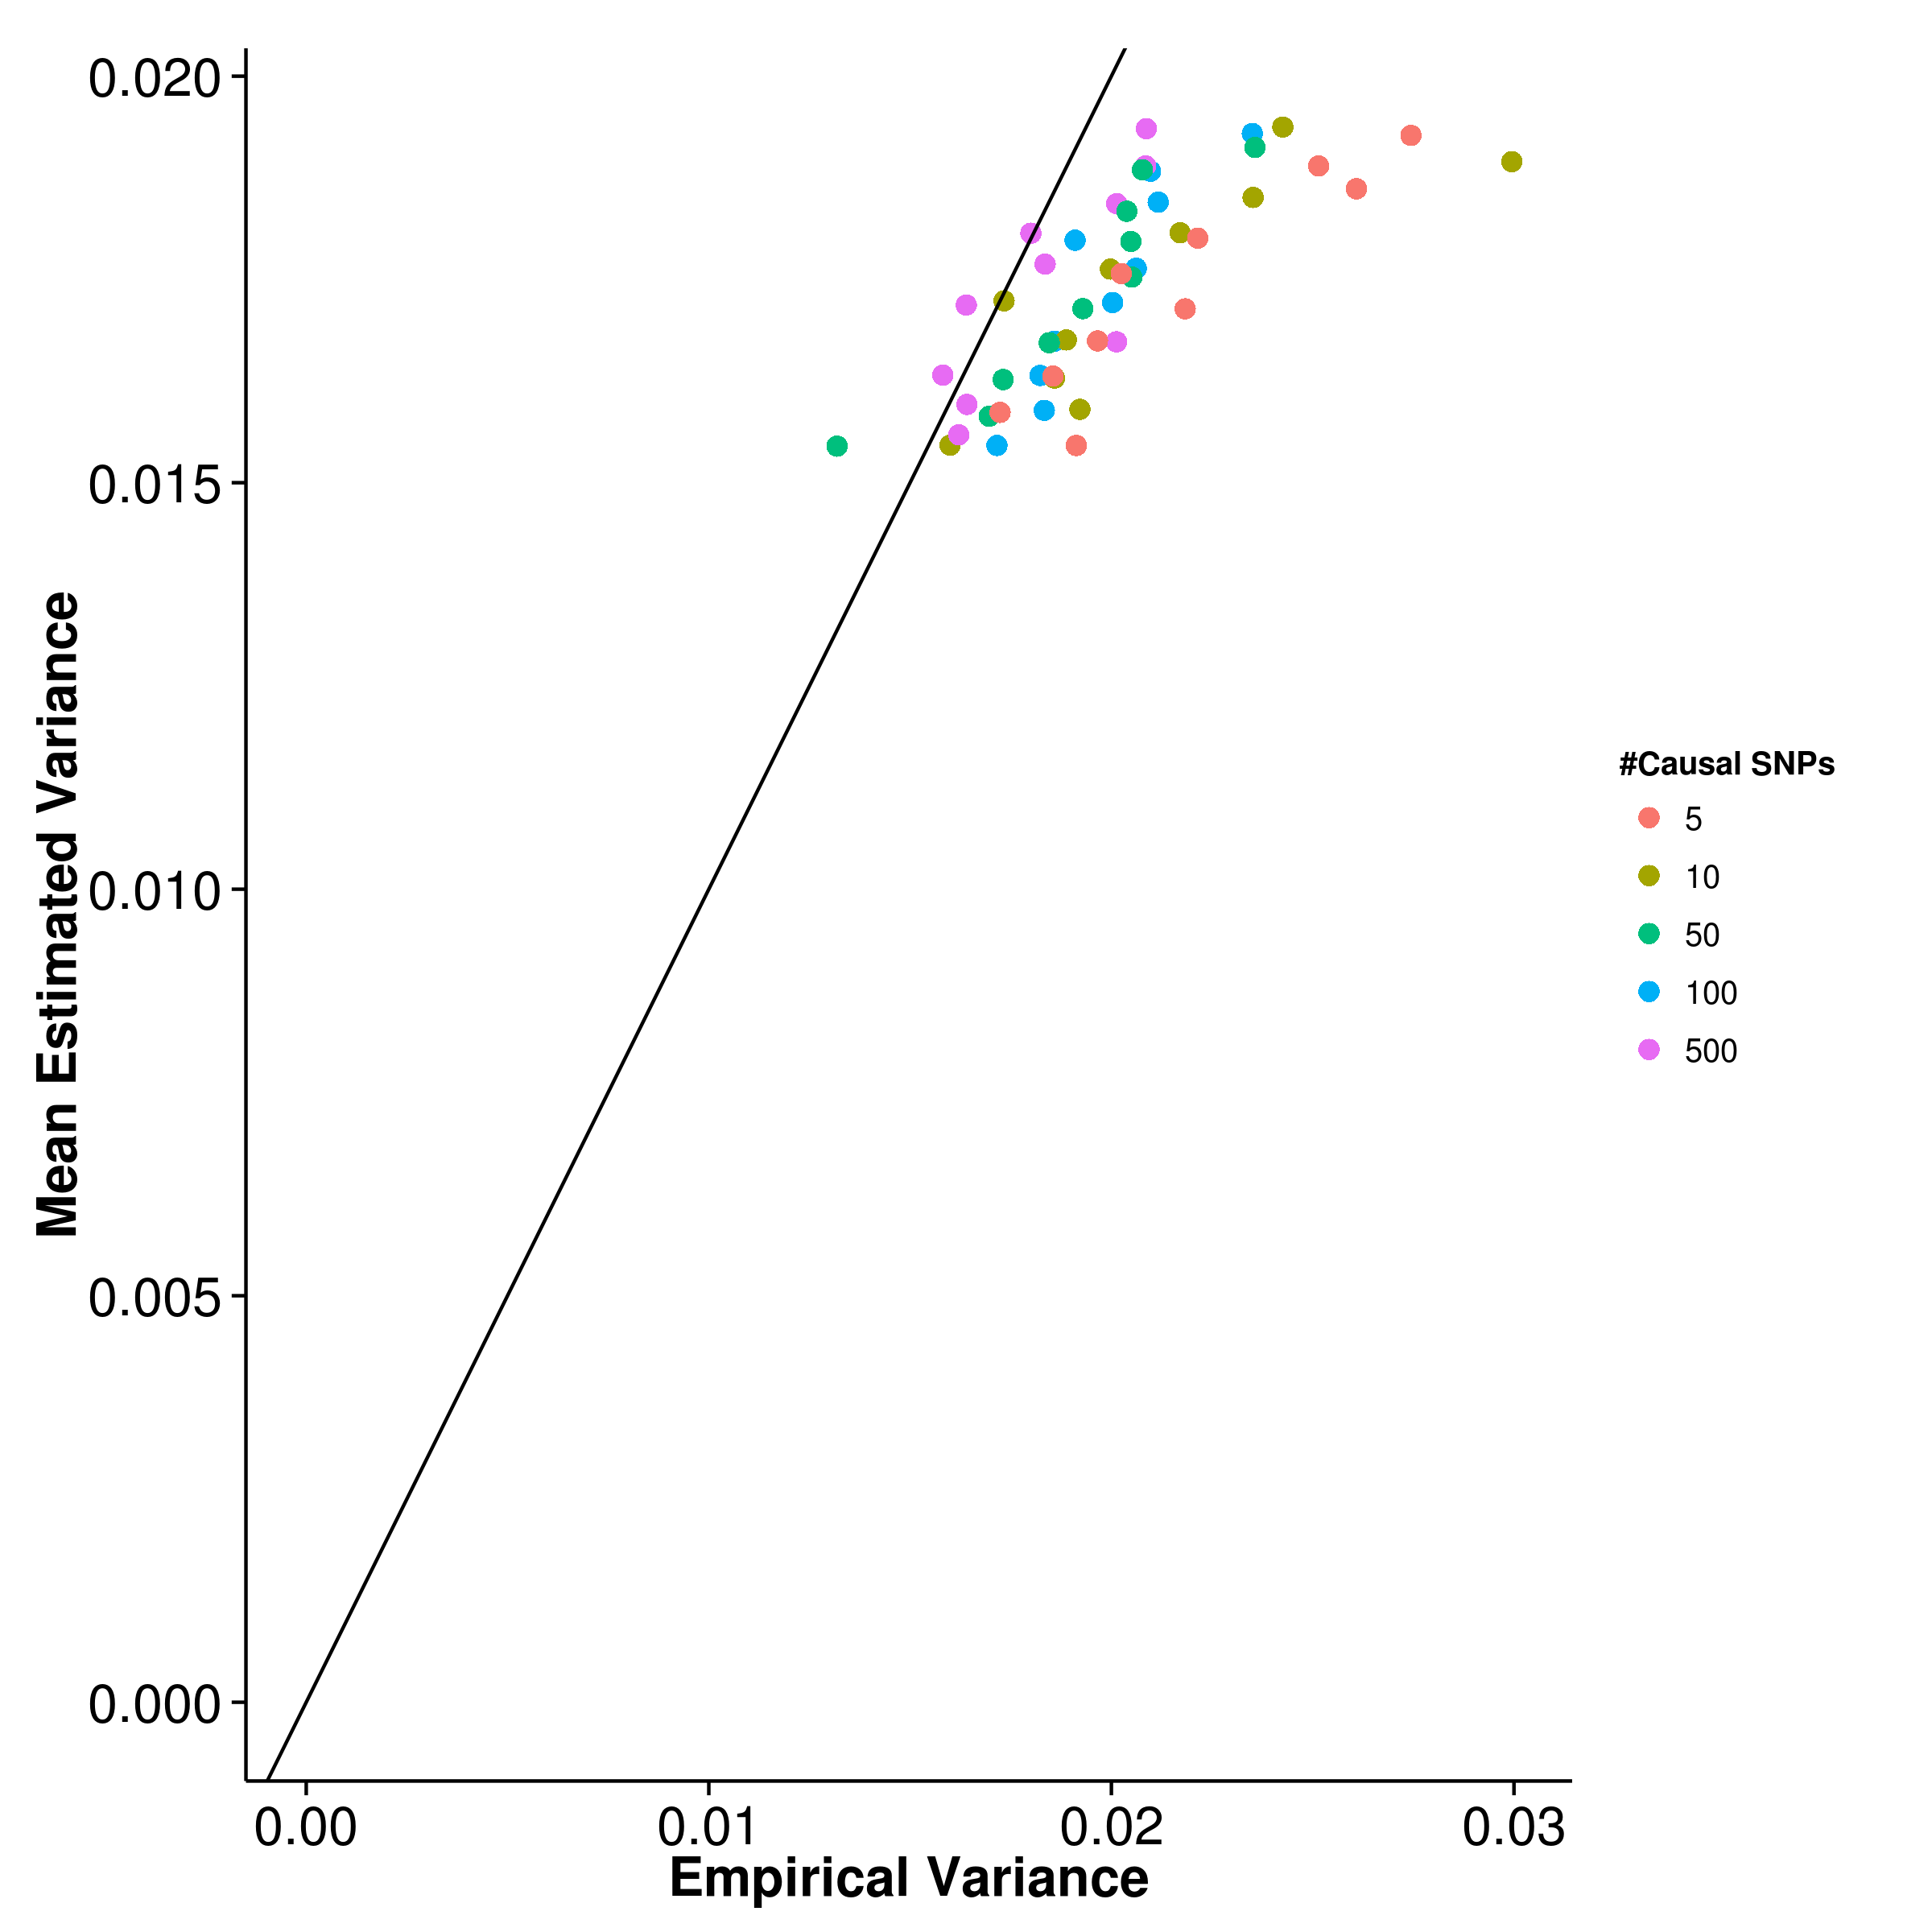
\includegraphics{figure/he_summary/random/shrek_Qt_Rand_sdCom.png}}
				\label{fig:shrekQtRandVarCom}
			}
			\subfloat[GCTA]{
				\scalebox{.4}{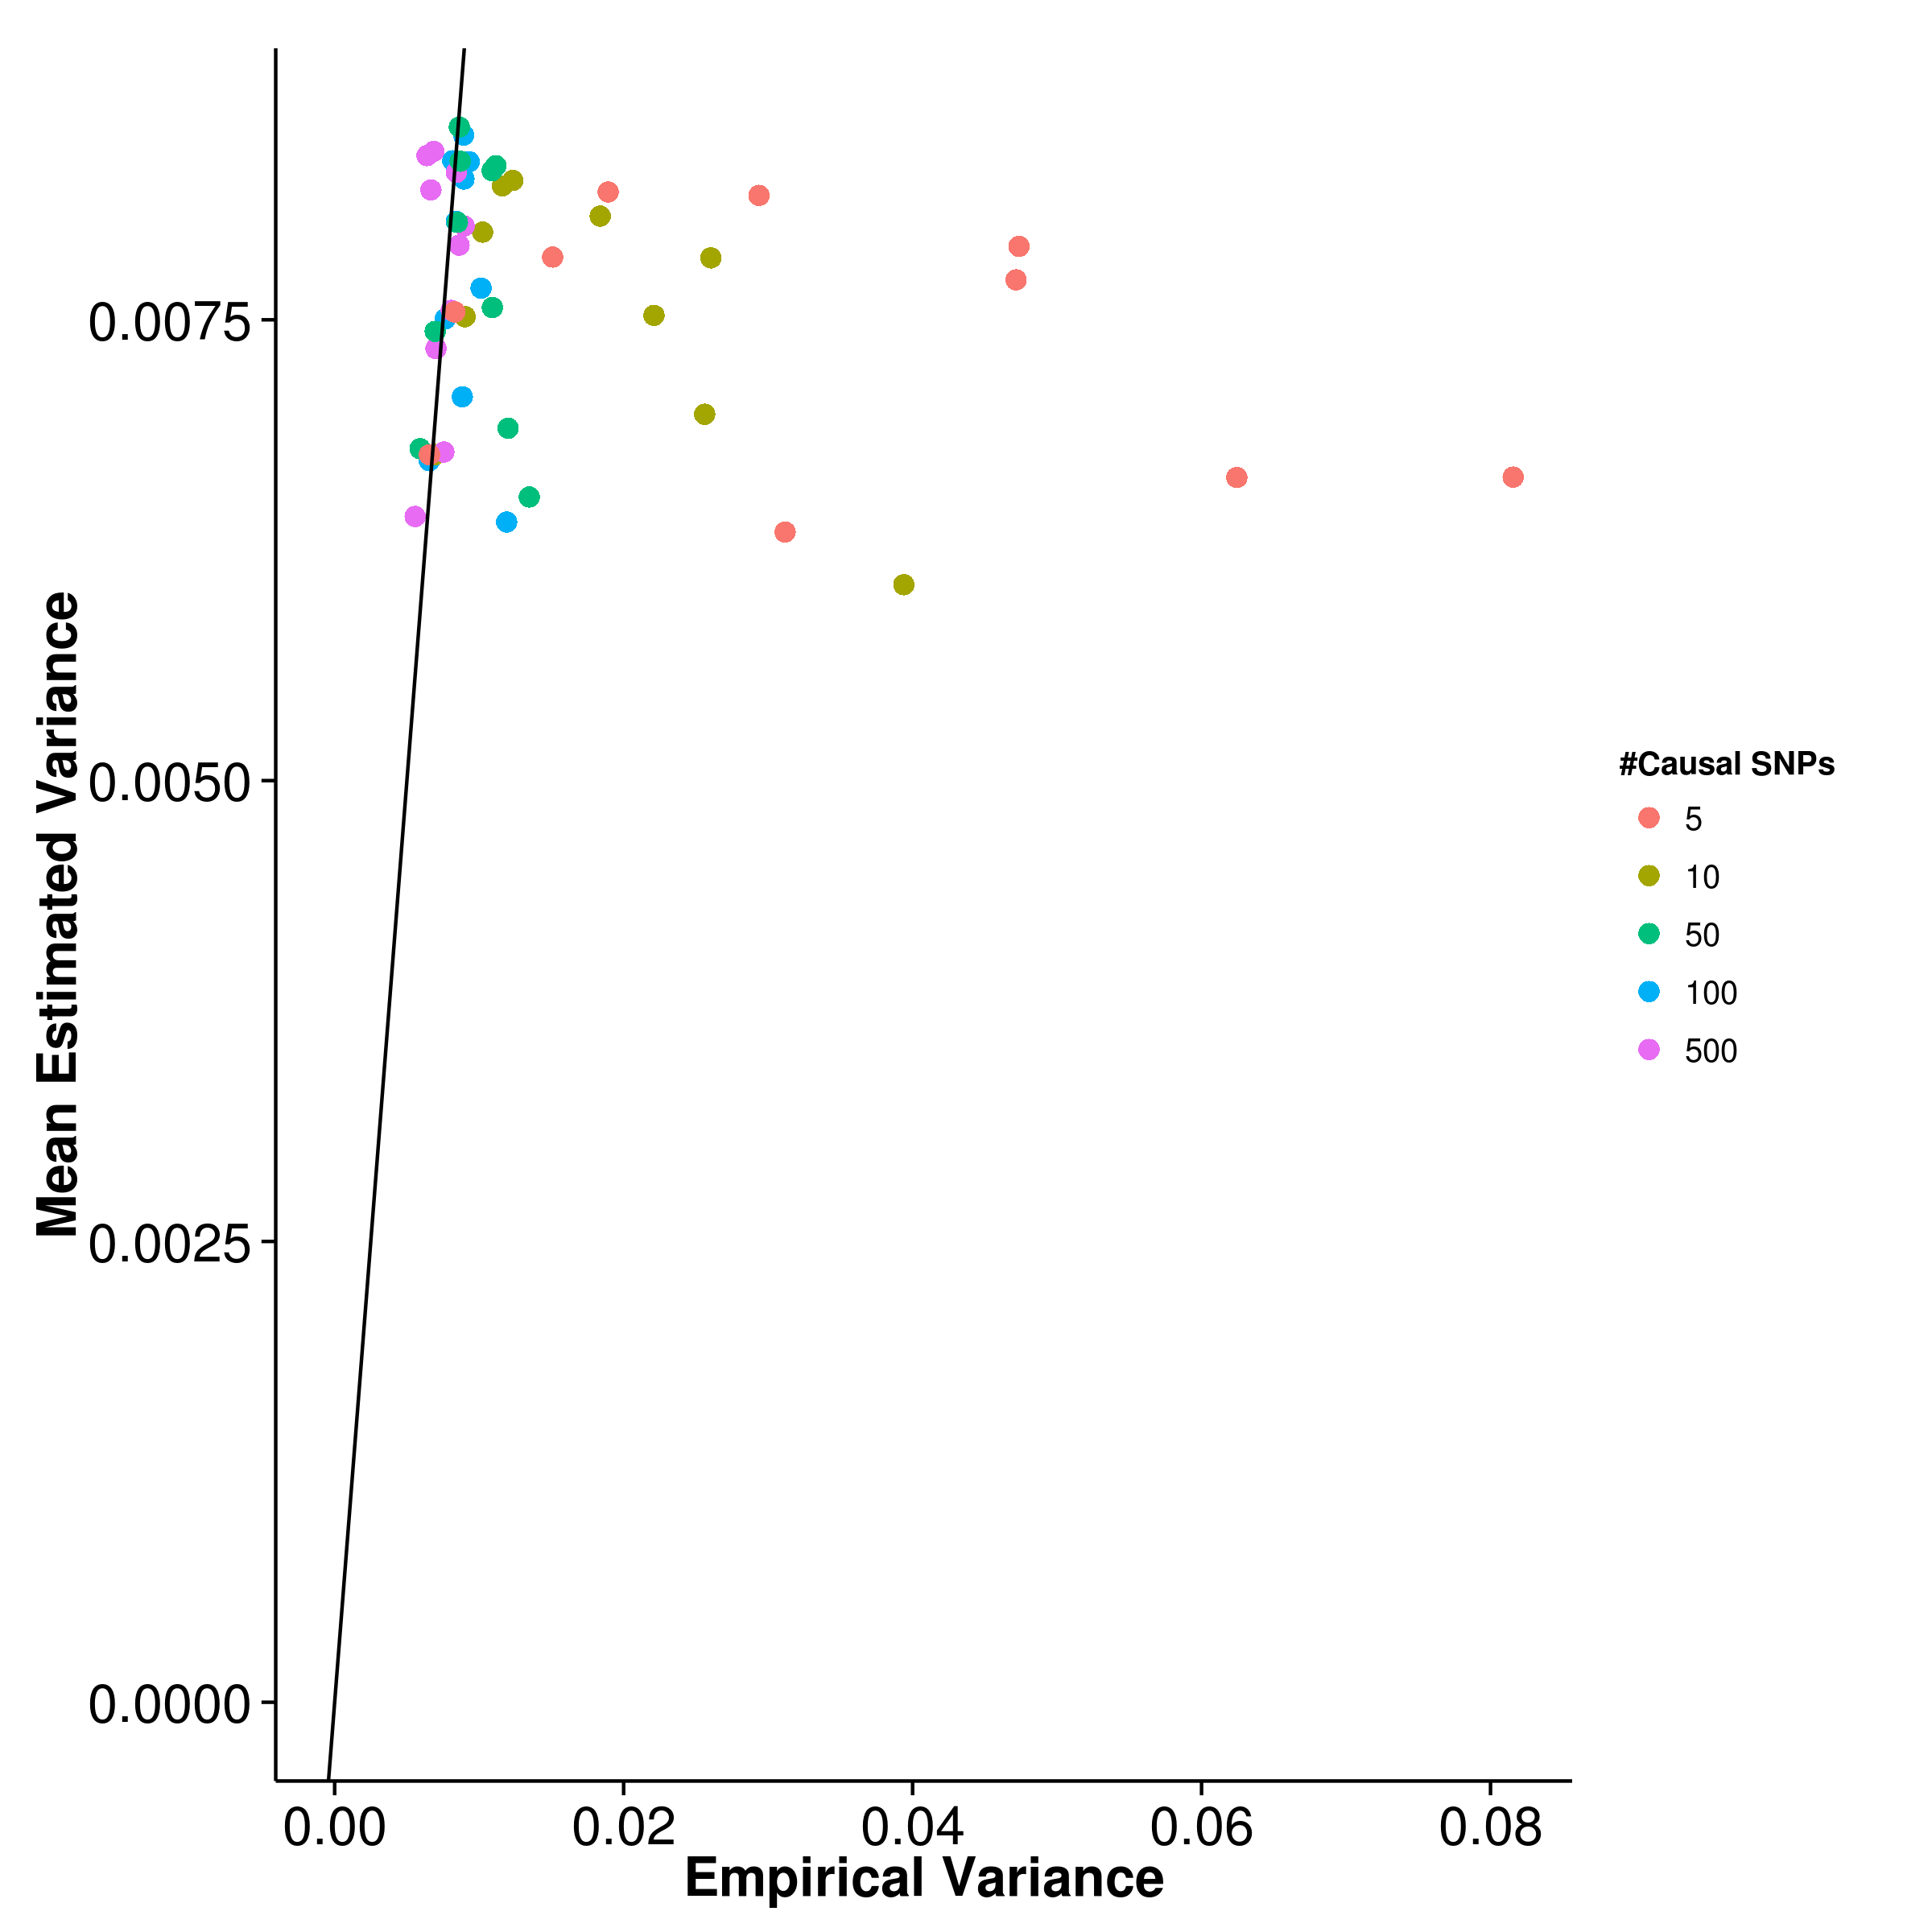
\includegraphics{figure/he_summary/random/gcta_Qt_Rand_sdCom.png}}
				\label{fig:gctaQtRandVarCom}
			}\\
			\subfloat[LDSC with fix intercept]{
				\scalebox{.4}{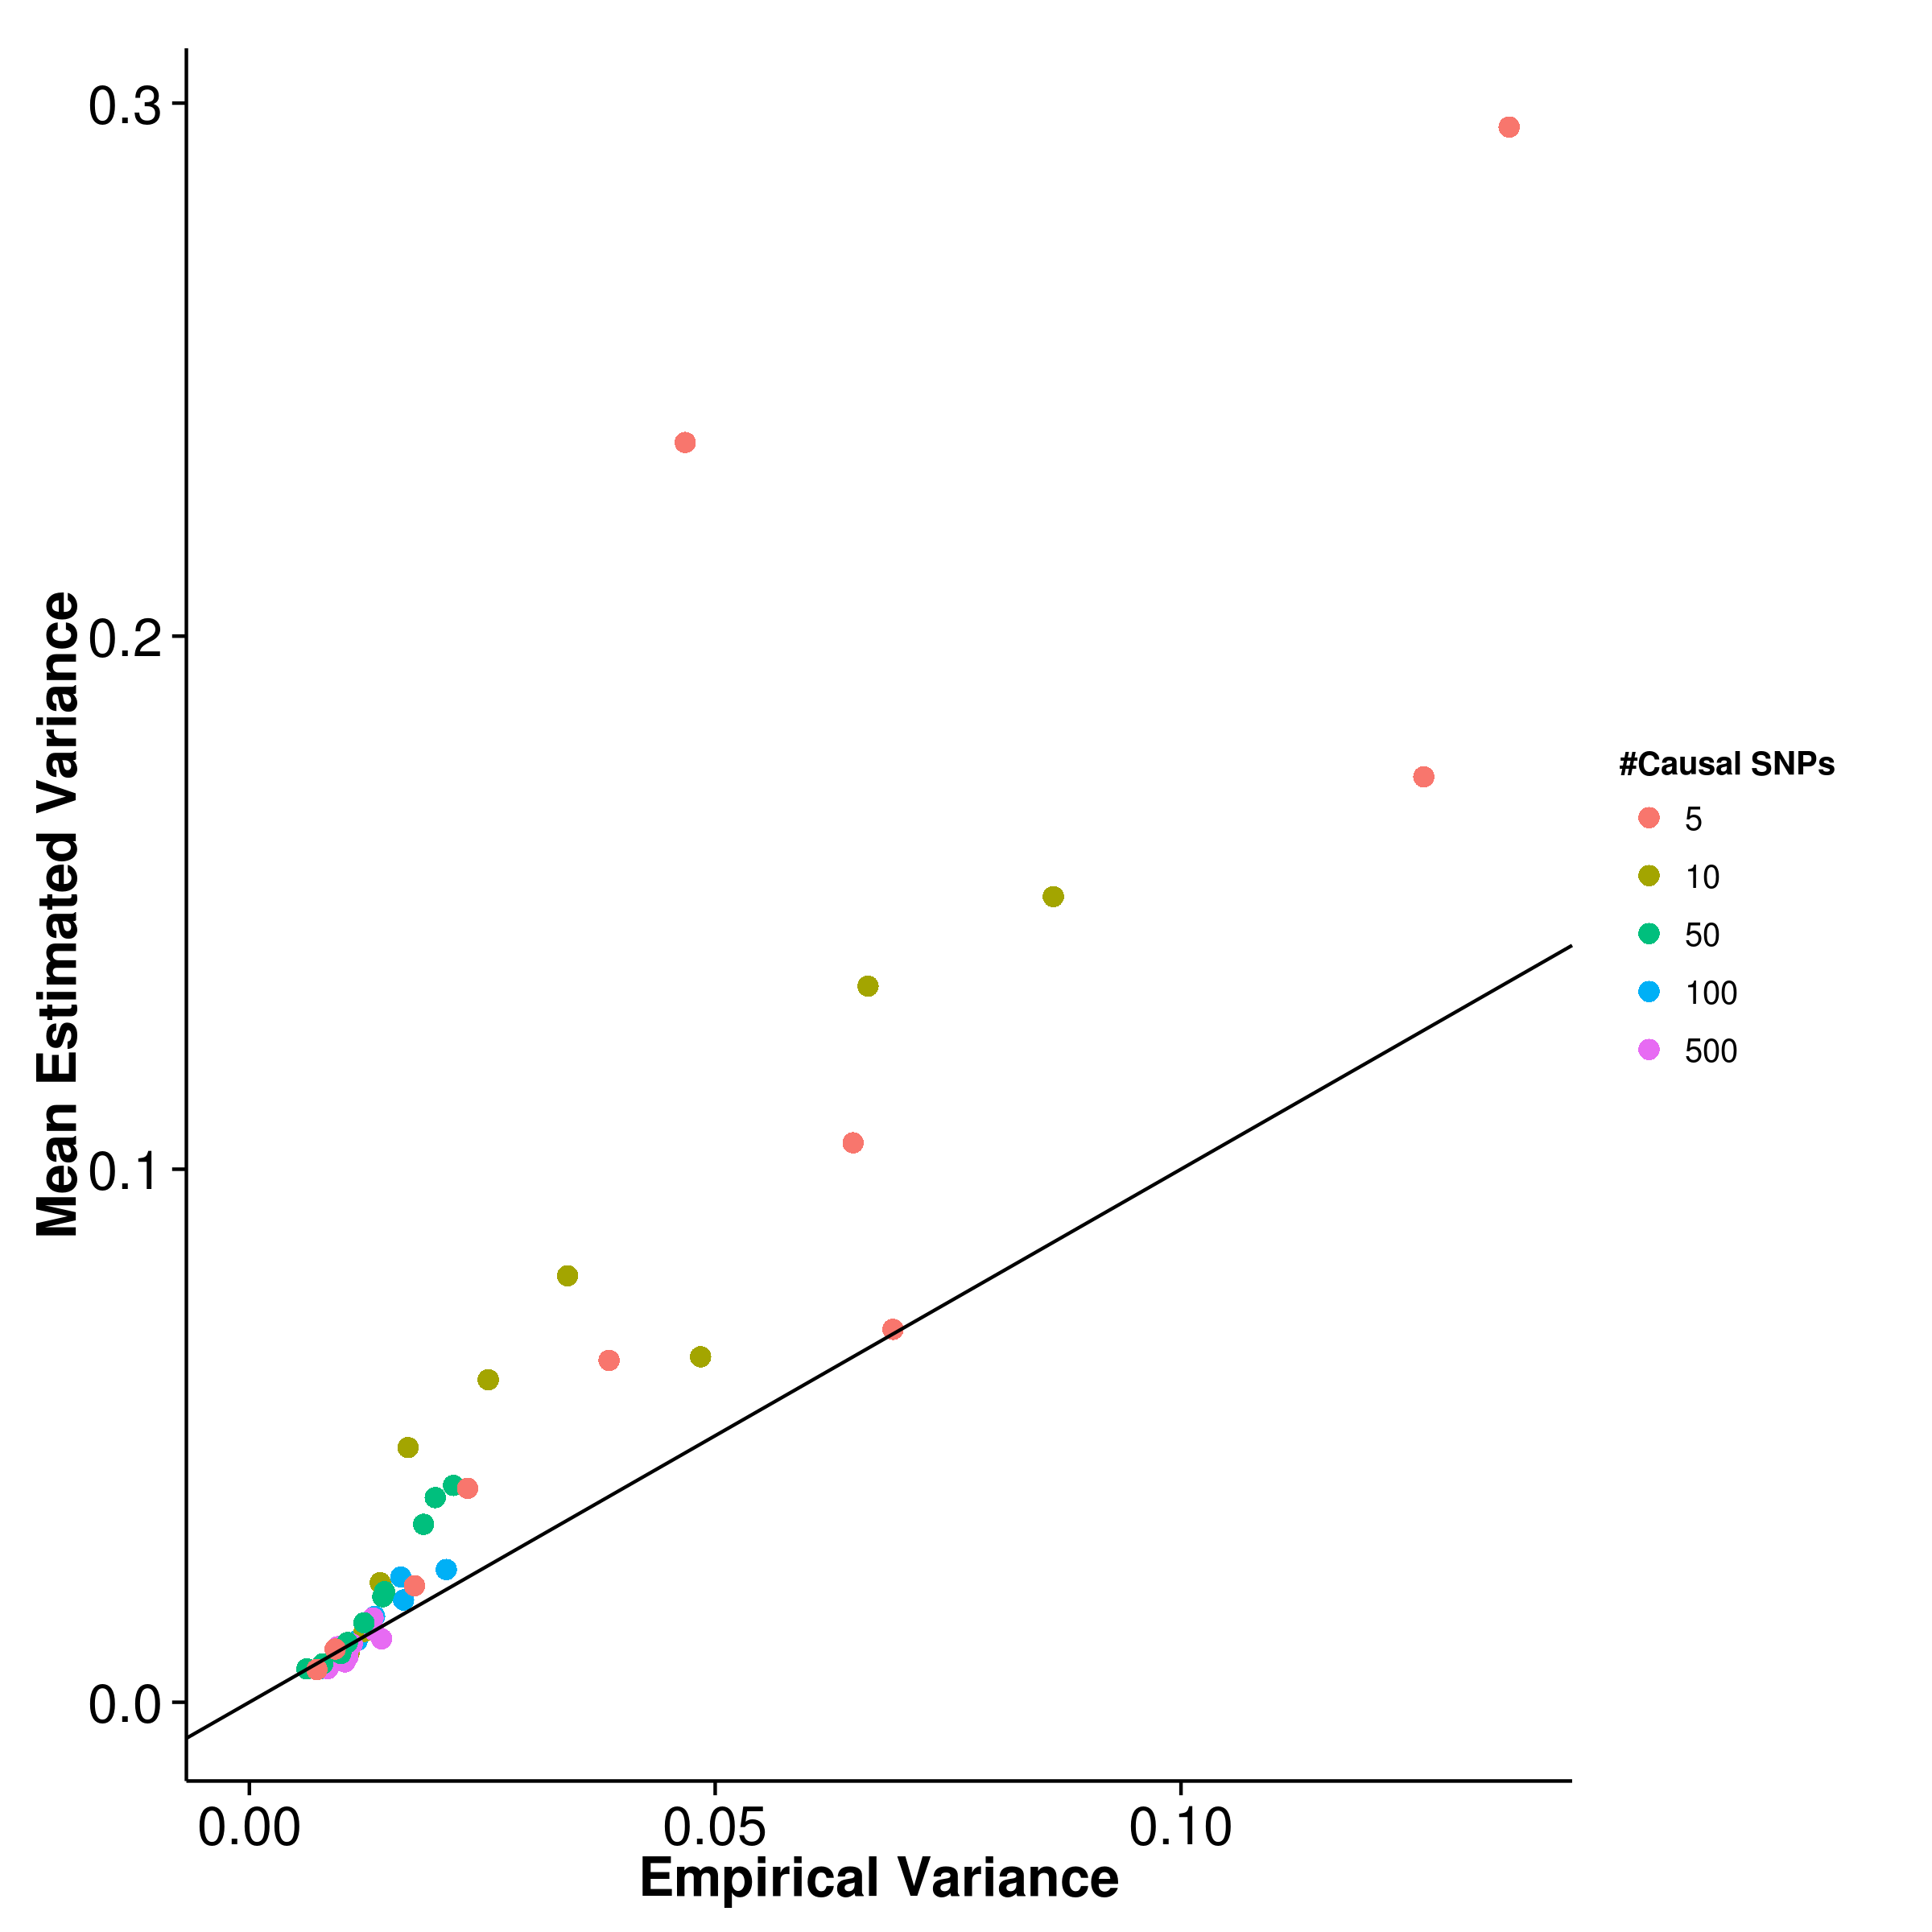
\includegraphics{figure/he_summary/random/ldsc_Qt_Rand_sdCom.png}}
				\label{fig:ldscQtRandVarCom}
			}
			\subfloat[LDSC with intercept estimation]{
				
				\scalebox{.4}{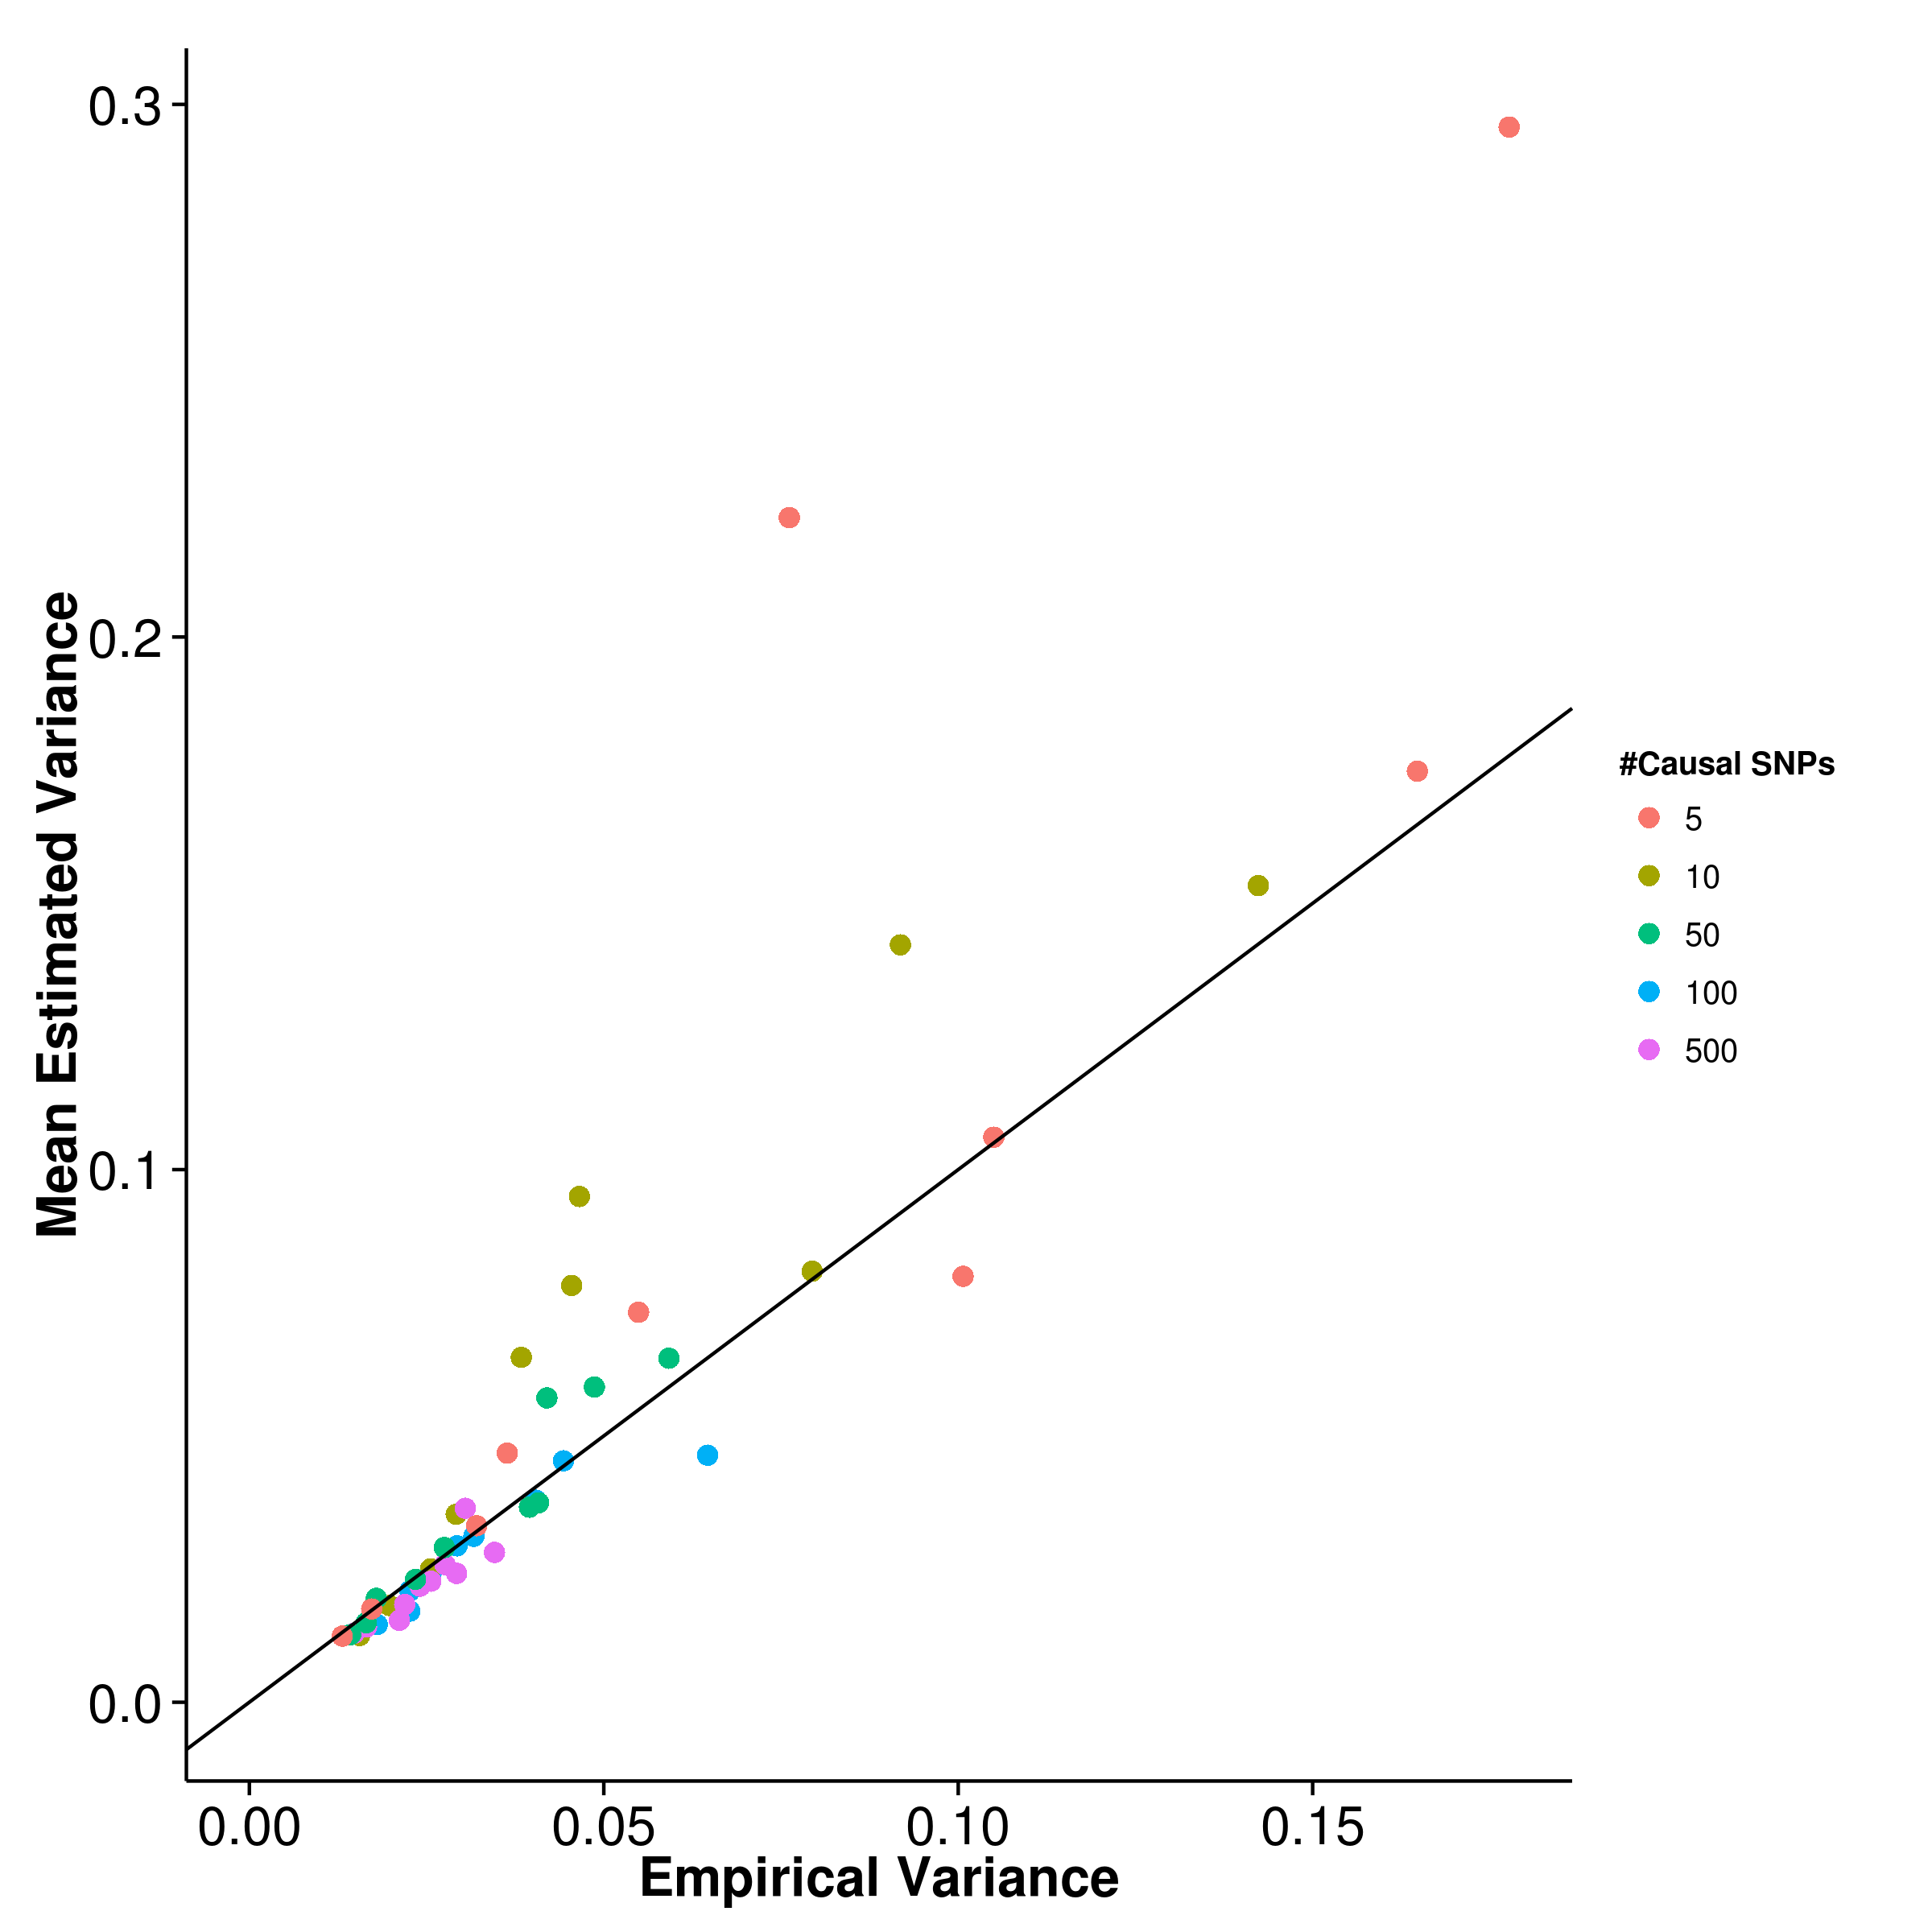
\includegraphics{figure/he_summary/random/ldscIn_Qt_Rand_sdCom.png}}
				\label{fig:ldscInQtRandVarCom}
			}
			\caption[Estimation of Variance in Quantitative Trait Simulation]
			{Estimated variance of results from quantitative trait simulation with random effect size simulation when compared to the empirical variance.
			\gls{gcta} has the best estimate of its empirical variance under the polygenic conditions whereas \gls{shrek} tends to under-estimate its empirical variance.
			On the other hand, \gls{ldsc} to over-estimate the variance especially when the number of causal \glspl{SNP} is small.
				} 
			\label{fig:QtRandVarCom}
		\end{figure}
		Next, we simulate quantitative trait with random effect size assigned to the causal \glspl{SNP}.
		The exponential distribution with $\lambda=1$ was selected because it was suggested that it may serve as a heuristic expectation the genetic architecture of adaptation\citep{Orr1998}.
		There might be many other distribution that can be used, however due to limitation in resources, we will only focus on the exponential distribution with $\lambda=1$.

		Under this simulation condition, it was observed that the mean estimation of heritability from \gls{shrek}(\cref{fig:shrekQtRandMean}) and \gls{gcta}(\cref{fig:gctaQtRandMean}) were similar to what was observed in the equal effect size simulation.
		For \gls{ldsc} with intercept estimation(\cref{fig:ldscInQtRandMean}), less bias was observed with only the 10 causal \glspl{SNP} scenario being under estimated. 
		On the other hand, the performance of \gls{ldsc} with fixed intercept remain more or less the same, with a larger degree of fluctuation when small number of causal \glspl{SNP}(5 or 10) was simulated. 
		The fluctuation in estimate can also be observed in the empirical variance of \gls{ldsc}(\cref{fig:ldscQtRandVar,fig:ldscInQtRandVar}).
		Despite the relative stable performance of \gls{gcta}, the empirical variance of \gls{gcta} also fluctuate when the number of causal \glspl{SNP} was small. 
		Such pattern was not observed in \gls{shrek} suggesting that it might be robust against the change in number of causal \glspl{SNP}.
		
		When inspecting the relationship between the estimated and empirical variance, it was observed all programmes have a less accurate estimation of its variance when there is only 5 causal \glspl{SNP}. 
		The difference was most obvious for \gls{gcta} where the under-estimation of variance under the oligo-genic scenario(5 or 10 causal \glspl{SNP}) was more severe when a random effect size was assigned to the causal \glspl{SNP}(\cref{fig:gctaQtRandVarCom}).    
		On the other hand, the degree of bias in estimating the variance remain more or less unchanged for \gls{shrek}(\cref{fig:shrekQtRandVarCom}) and \gls{ldsc} with intercept estimation(\cref{fig:ldscInQtRandVarCom}), with roughly 0.9 and 1.25 times difference from the empirical variance respectively.
		However, for \gls{ldsc} with fixed intercept(\cref{fig:ldscQtRandVarCom}), the fold difference increased slightly, changed from 1.5 fold difference to 1.65 fold difference.
		
		Overall, simulating the effect size using the exponential distribution only slightly increases the \gls{mse} of the programmes when the number of causal \glspl{SNP} is small and decreases the \gls{mse} when the number of causal \glspl{SNP} is larger. 
		Taking into considering of both the bias and standard error, \gls{shrek} has the better performance over \gls{ldsc} except when the trait is extremely polygenic(e.g. $\ge500$ causal \glspl{SNP}).
		\begin{table}
			\centering
			\begin{tabular}{rrrrr}
				\toprule
				Number of Causal SNPs&	SHREK&	LDSC&	LDSC-In&	GCTA \\
				\midrule
				5	&	0.177	&	0.565	&	0.584	&	0.230\\
				10	&	0.159	&	0.251	&	0.470	&	0.151\\
				50	&	0.153	&	0.179	&	0.378	&	0.0796\\
				100	&	0.157	&	0.166	&	0.305	&	0.0794\\
				250	&	0.152	&	0.144	&	0.266	&	0.0674\\
				500	&	0.143	&	0.134	&	0.247	&	0.0646\\
				\bottomrule
			\end{tabular}
			\caption[Mean Squared Error of Quantitative Trait Simulation with Random Effect Size]{
				\gls{mse} of quantitative trait simulation with random effect size.
				Again, \gls{gcta} has the lowest \gls{mse} except when there is only 5 causal \glspl{SNP} and the performance of \gls{shrek} and \gls{ldsc} with fix intercept converges as number of causal \glspl{SNP} increases. 
				\gls{ldsc} with fix intercept even surpassed \gls{shrek}'s performance when the number of causal \glspl{SNP} was as high as 500.}
			\label{tab:mseQtRandom}
		\end{table}
		% Extreme with 100 causal
		\subsection{Quantitative Trait Simulation with Extreme Effect Size}
		
		\begin{figure}
			\centering
			\subfloat[SHREK]{
				\scalebox{.4}{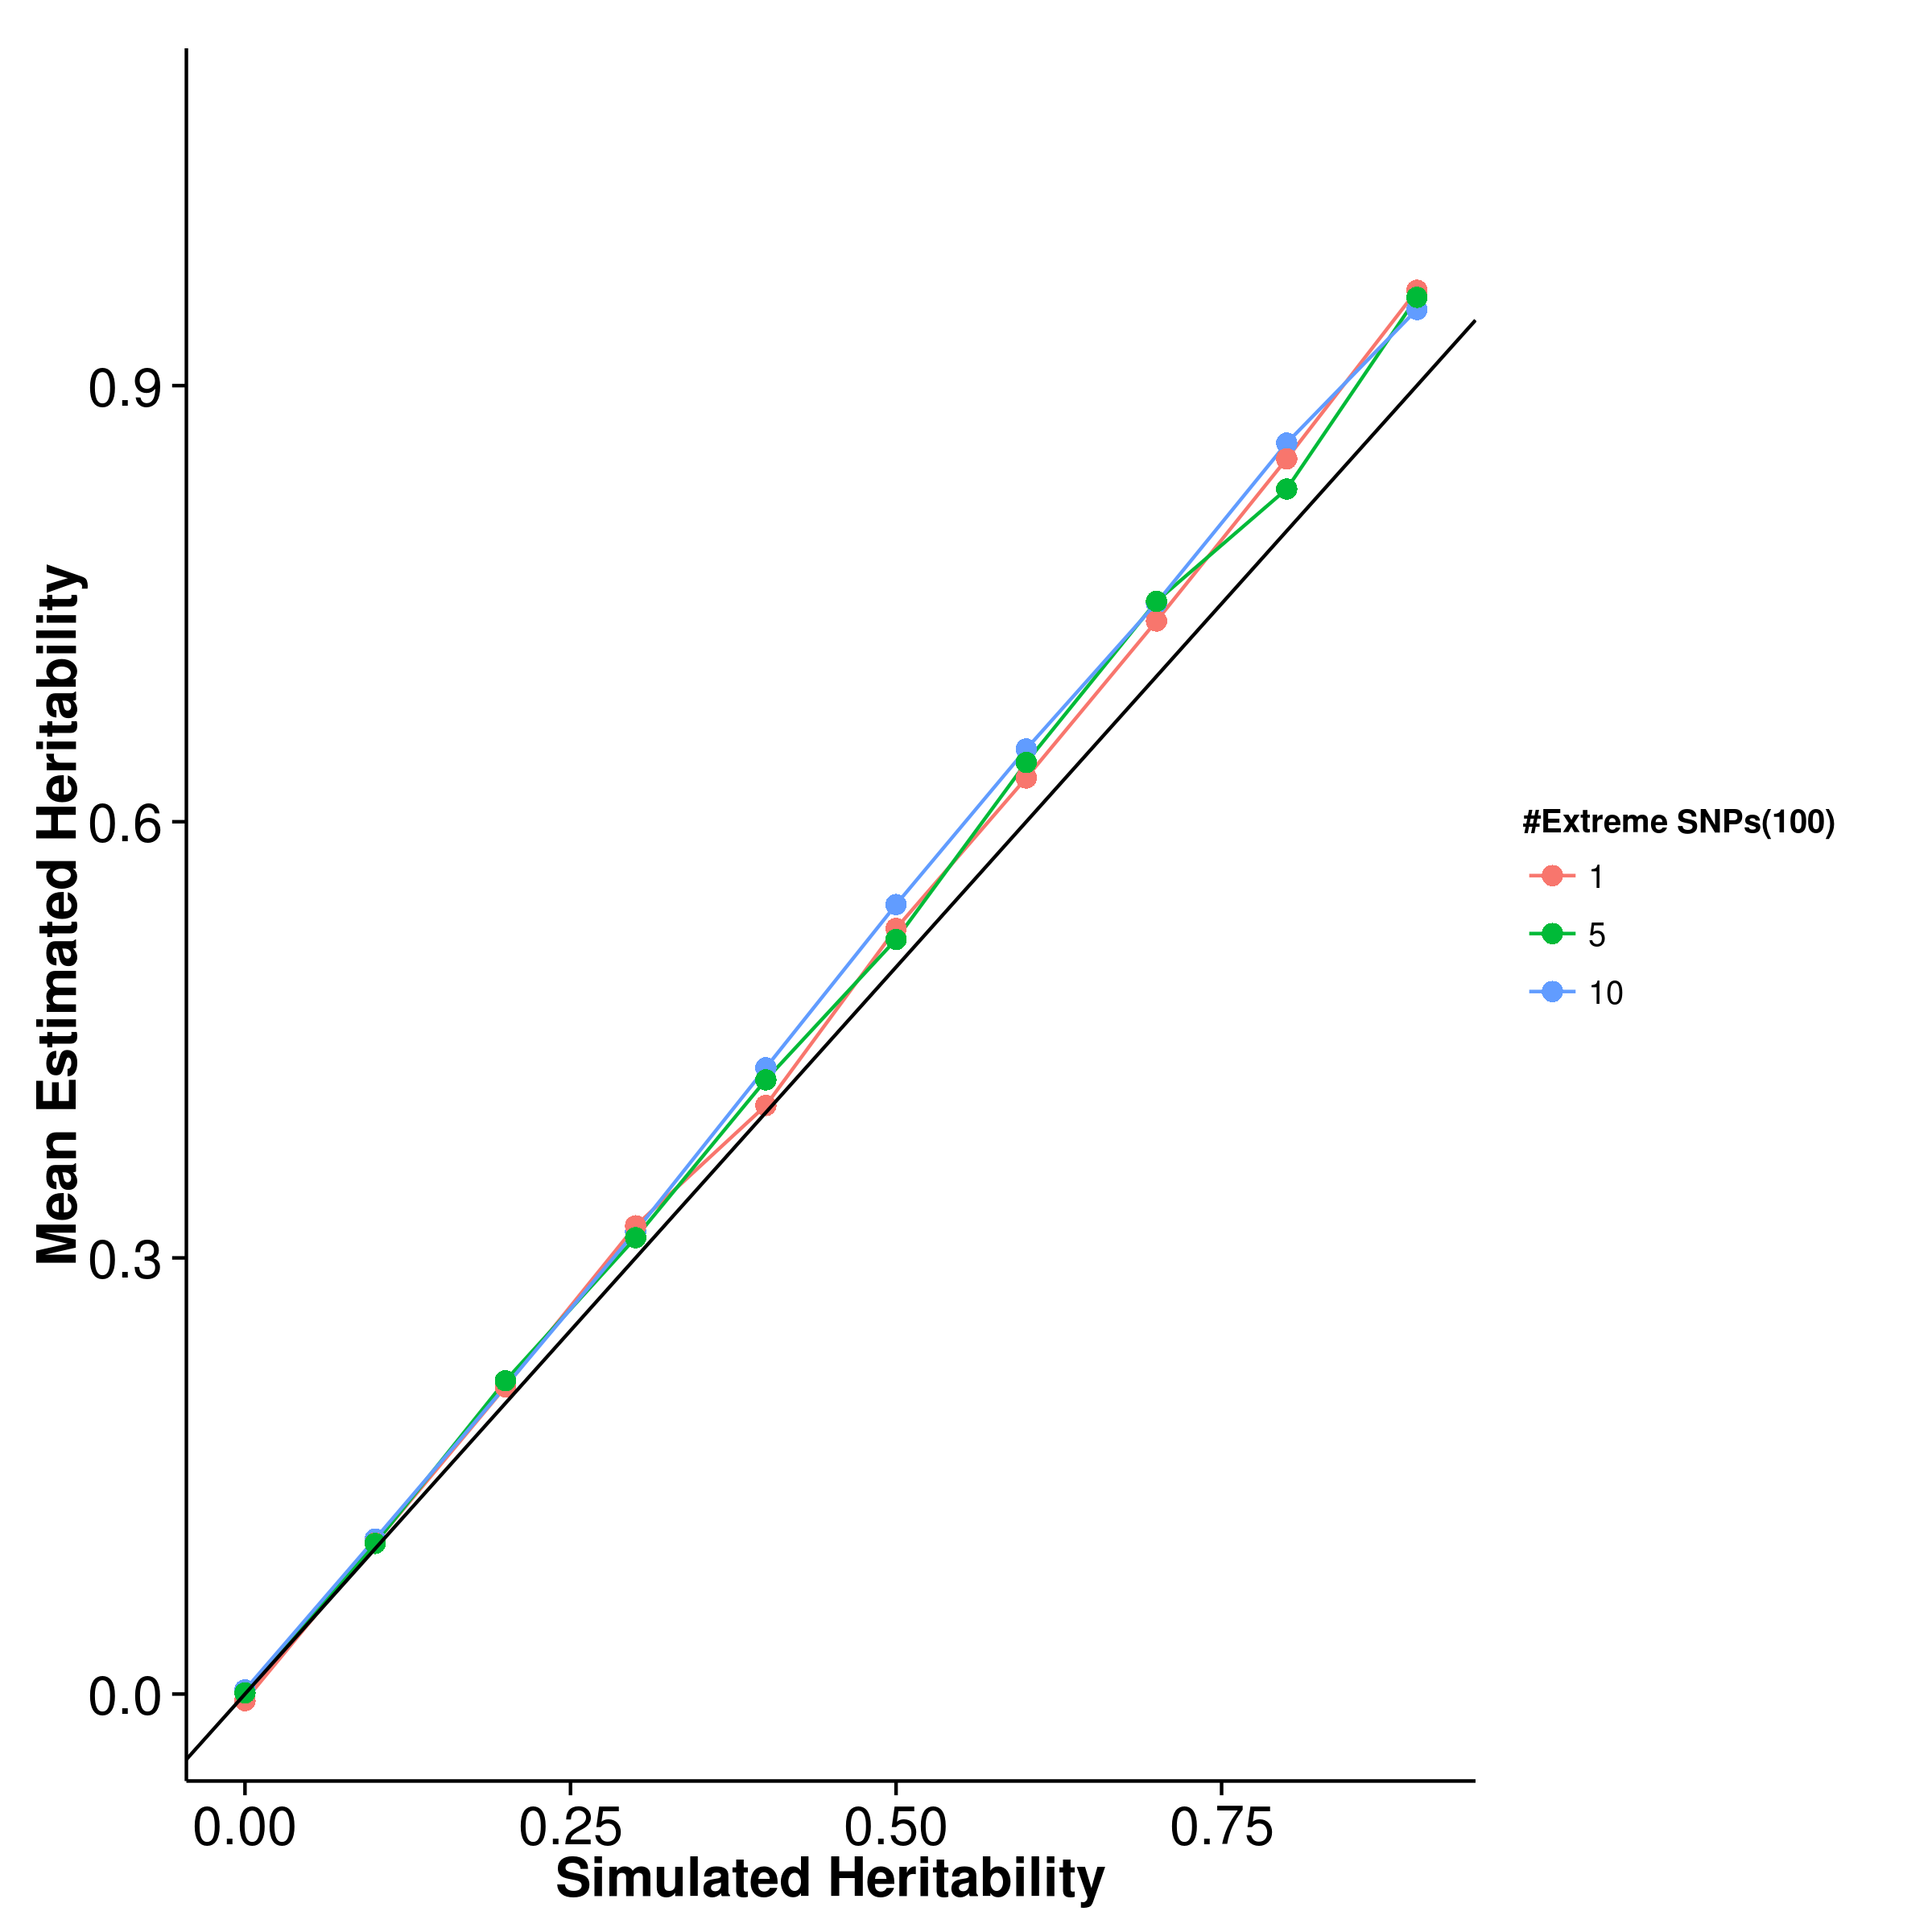
\includegraphics{figure/he_summary/extreme_100c/shrek_QtE_Rand_mean.png}}
				\label{fig:shrekQtEx100cMean}
			}
			\subfloat[GCTA]{
				\scalebox{.4}{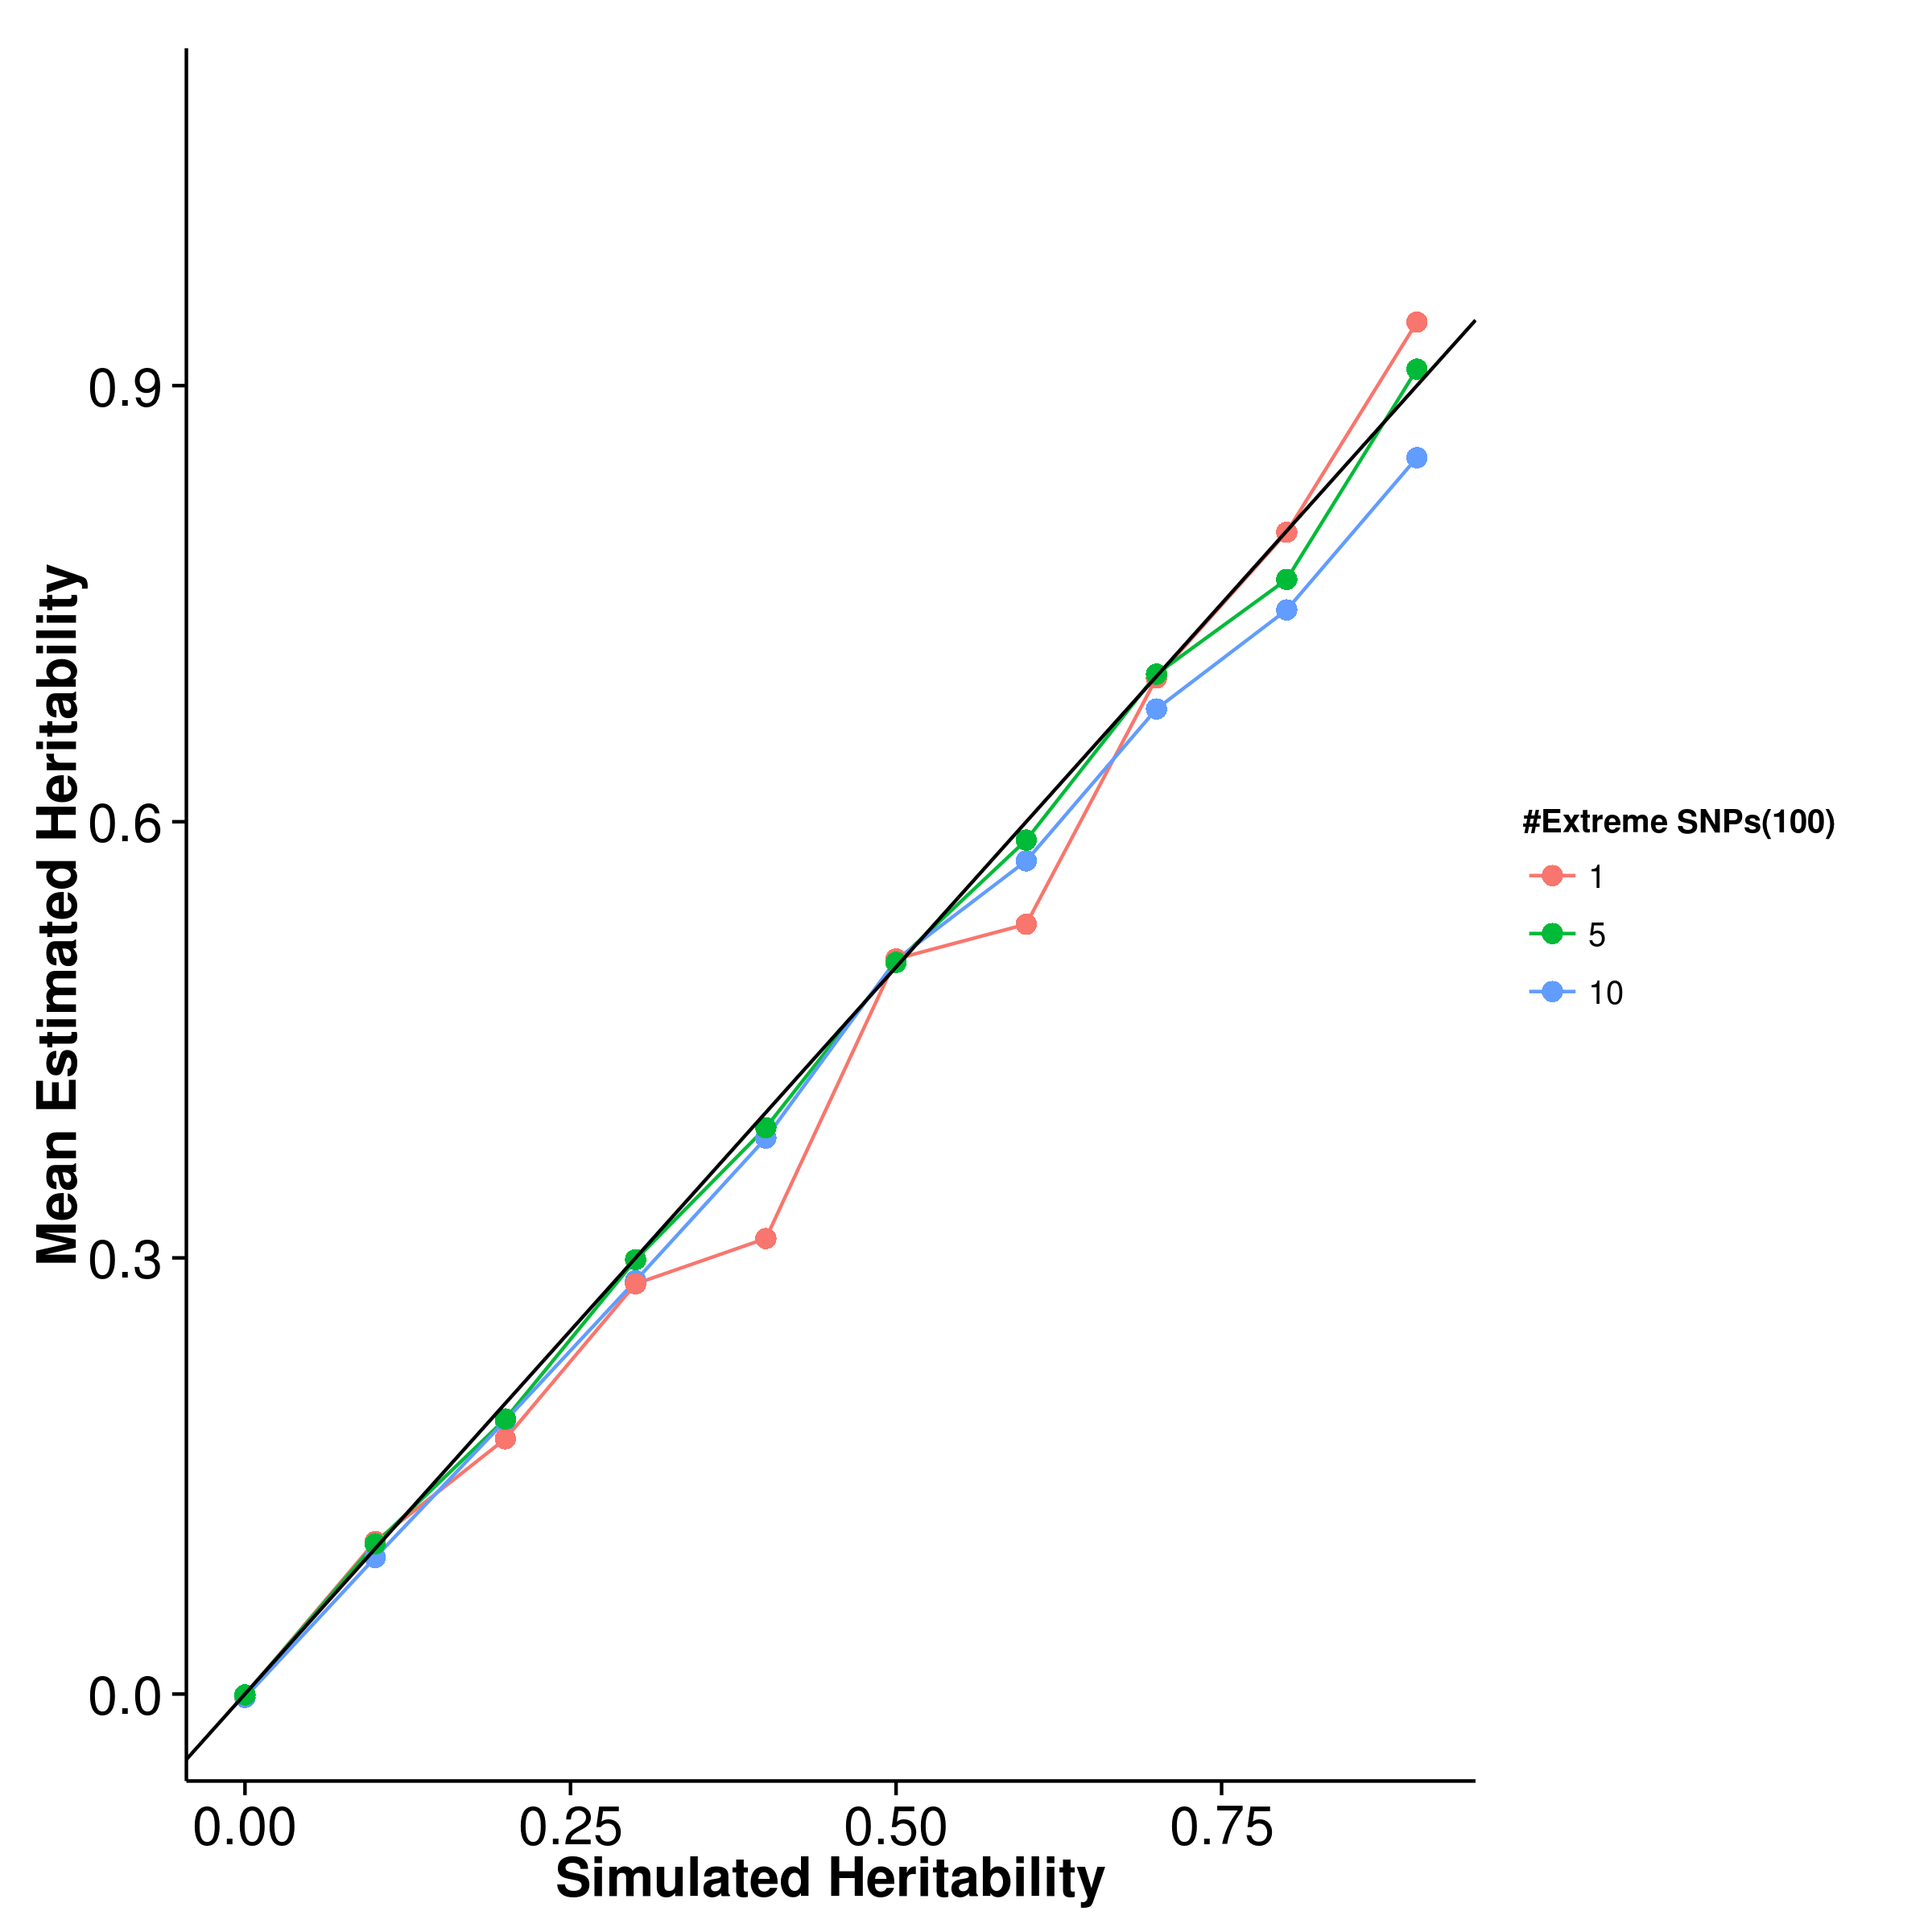
\includegraphics{figure/he_summary/extreme_100c/gcta_QtE_Rand_mean.png}}
				\label{fig:gctaQtEx100cMean}
			}\\
			\subfloat[LDSC with fix intercept]{
				\scalebox{.4}{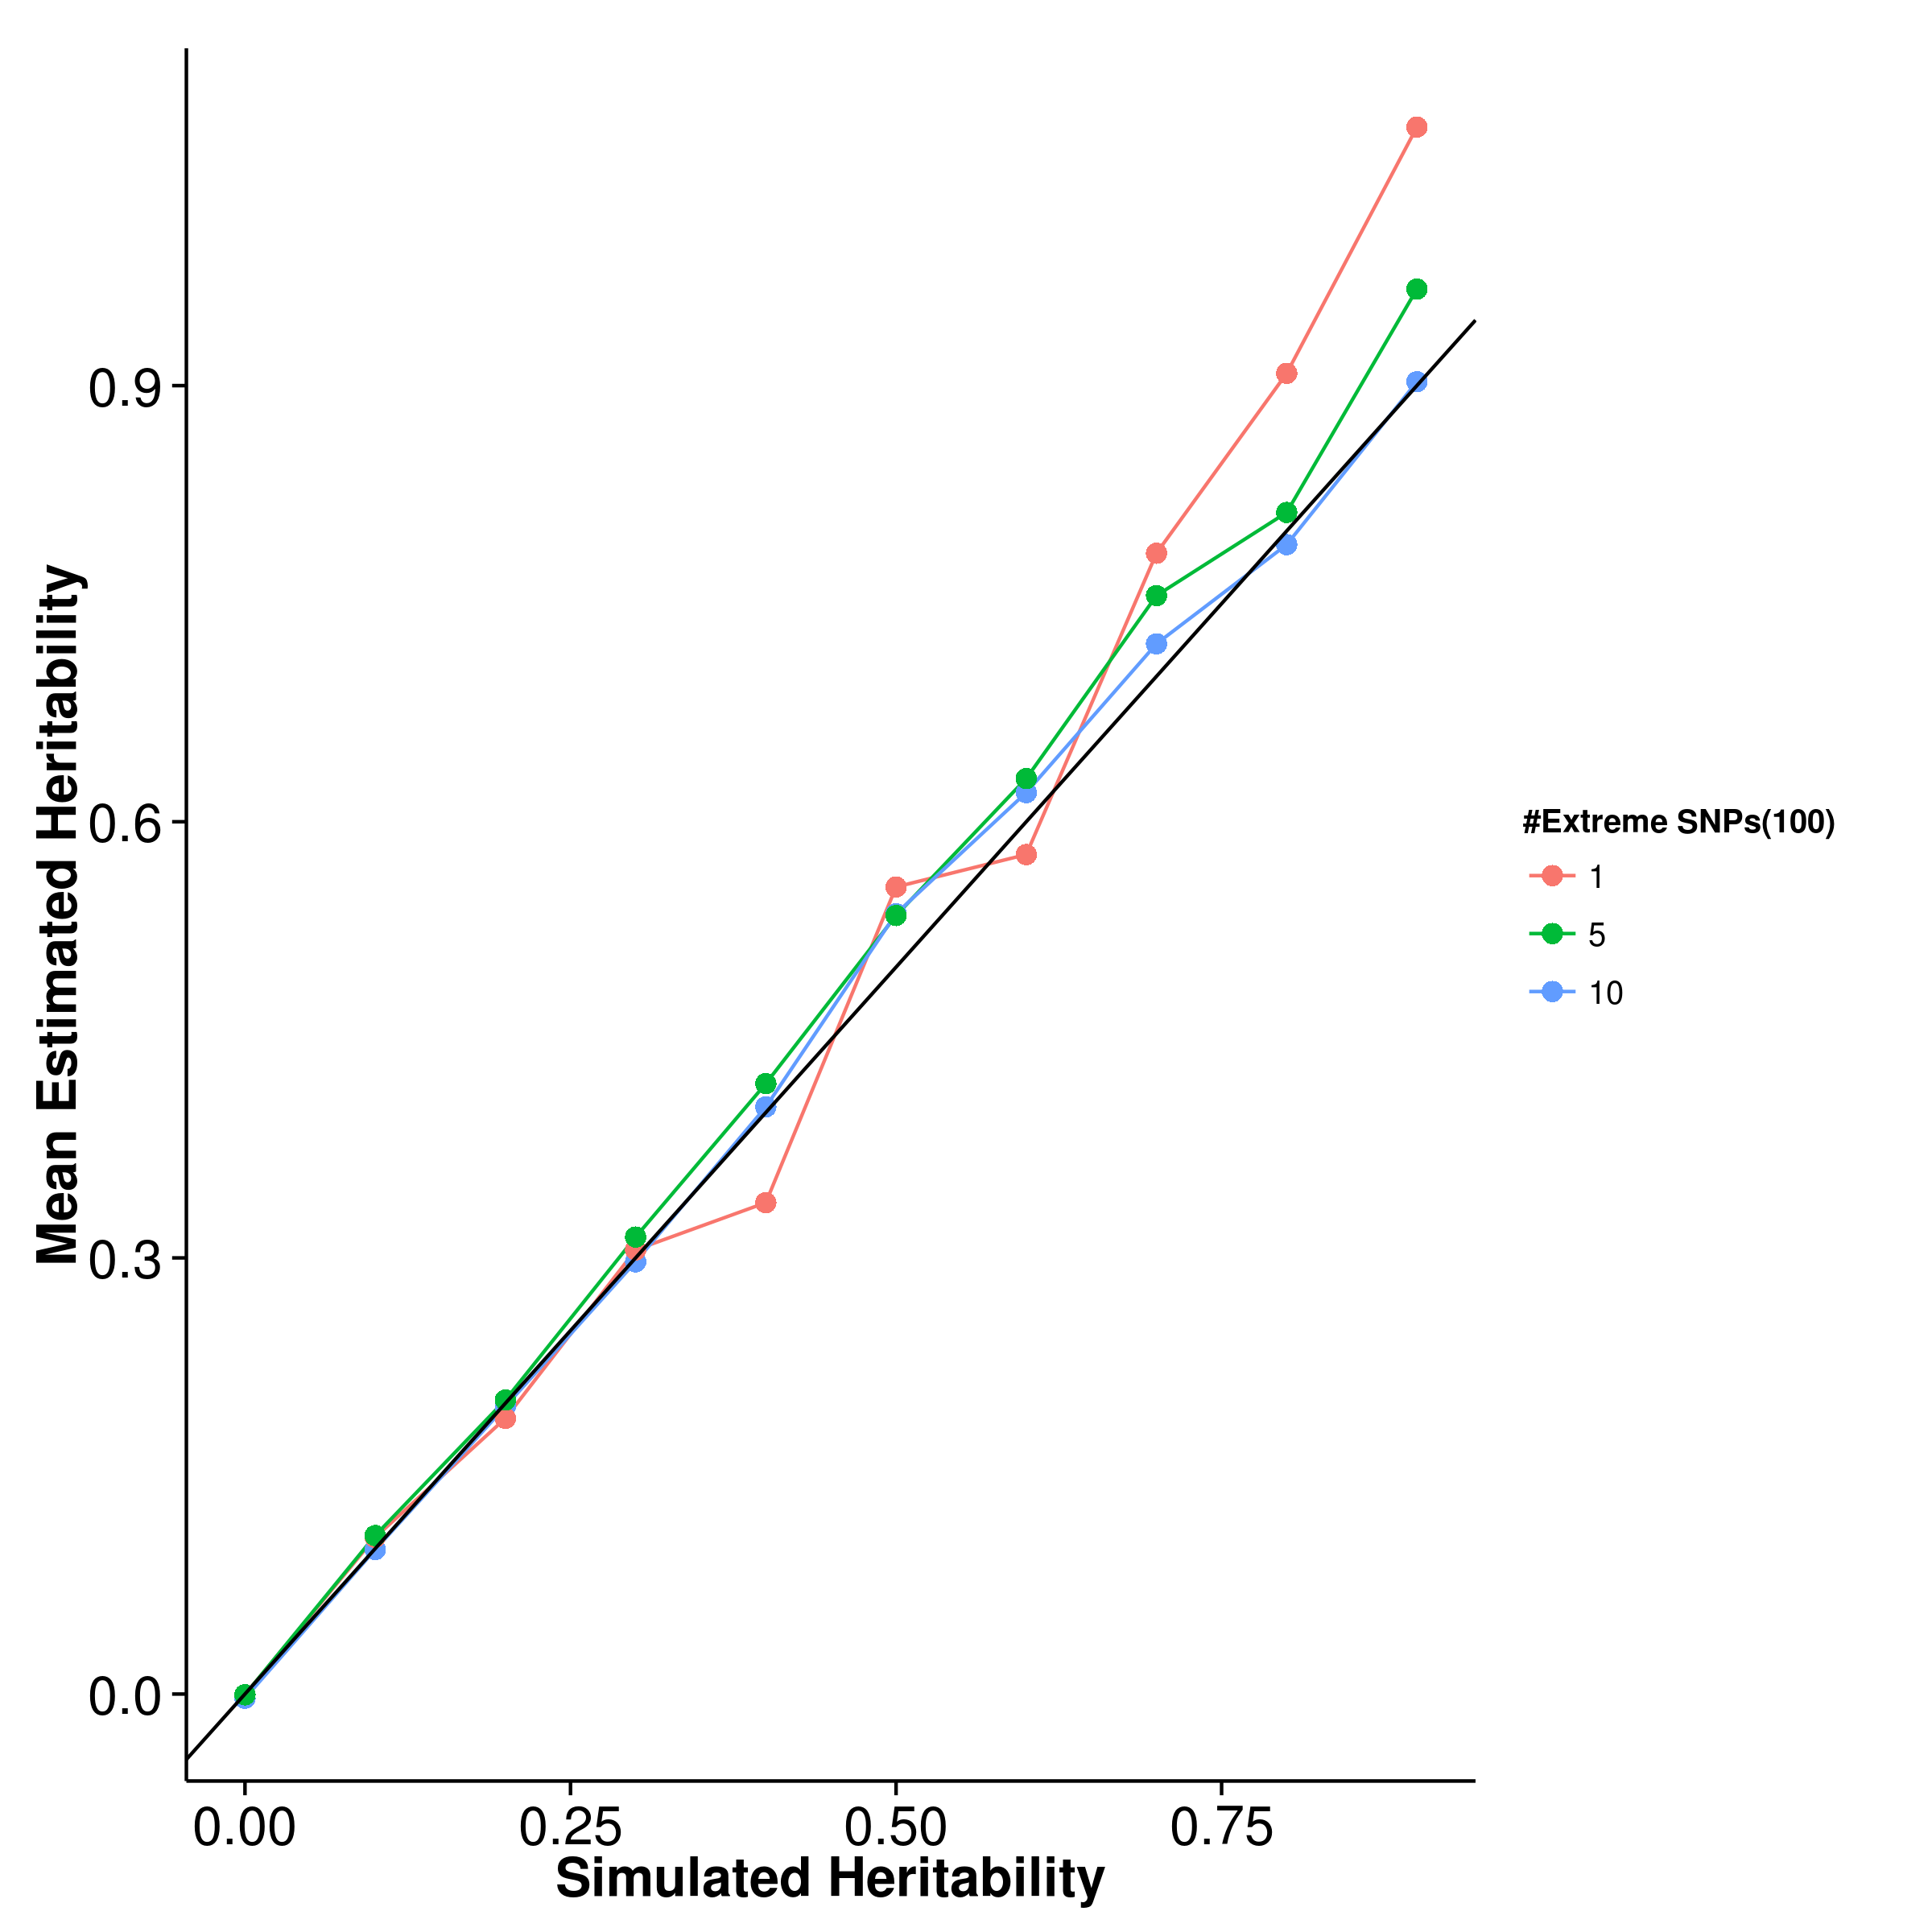
\includegraphics{figure/he_summary/extreme_100c/ldsc_QtE_Rand_mean.png}}
				\label{fig:ldscQtEx100cMean}
			}
			\subfloat[LDSC with intercept estimation]{
				
				\scalebox{.4}{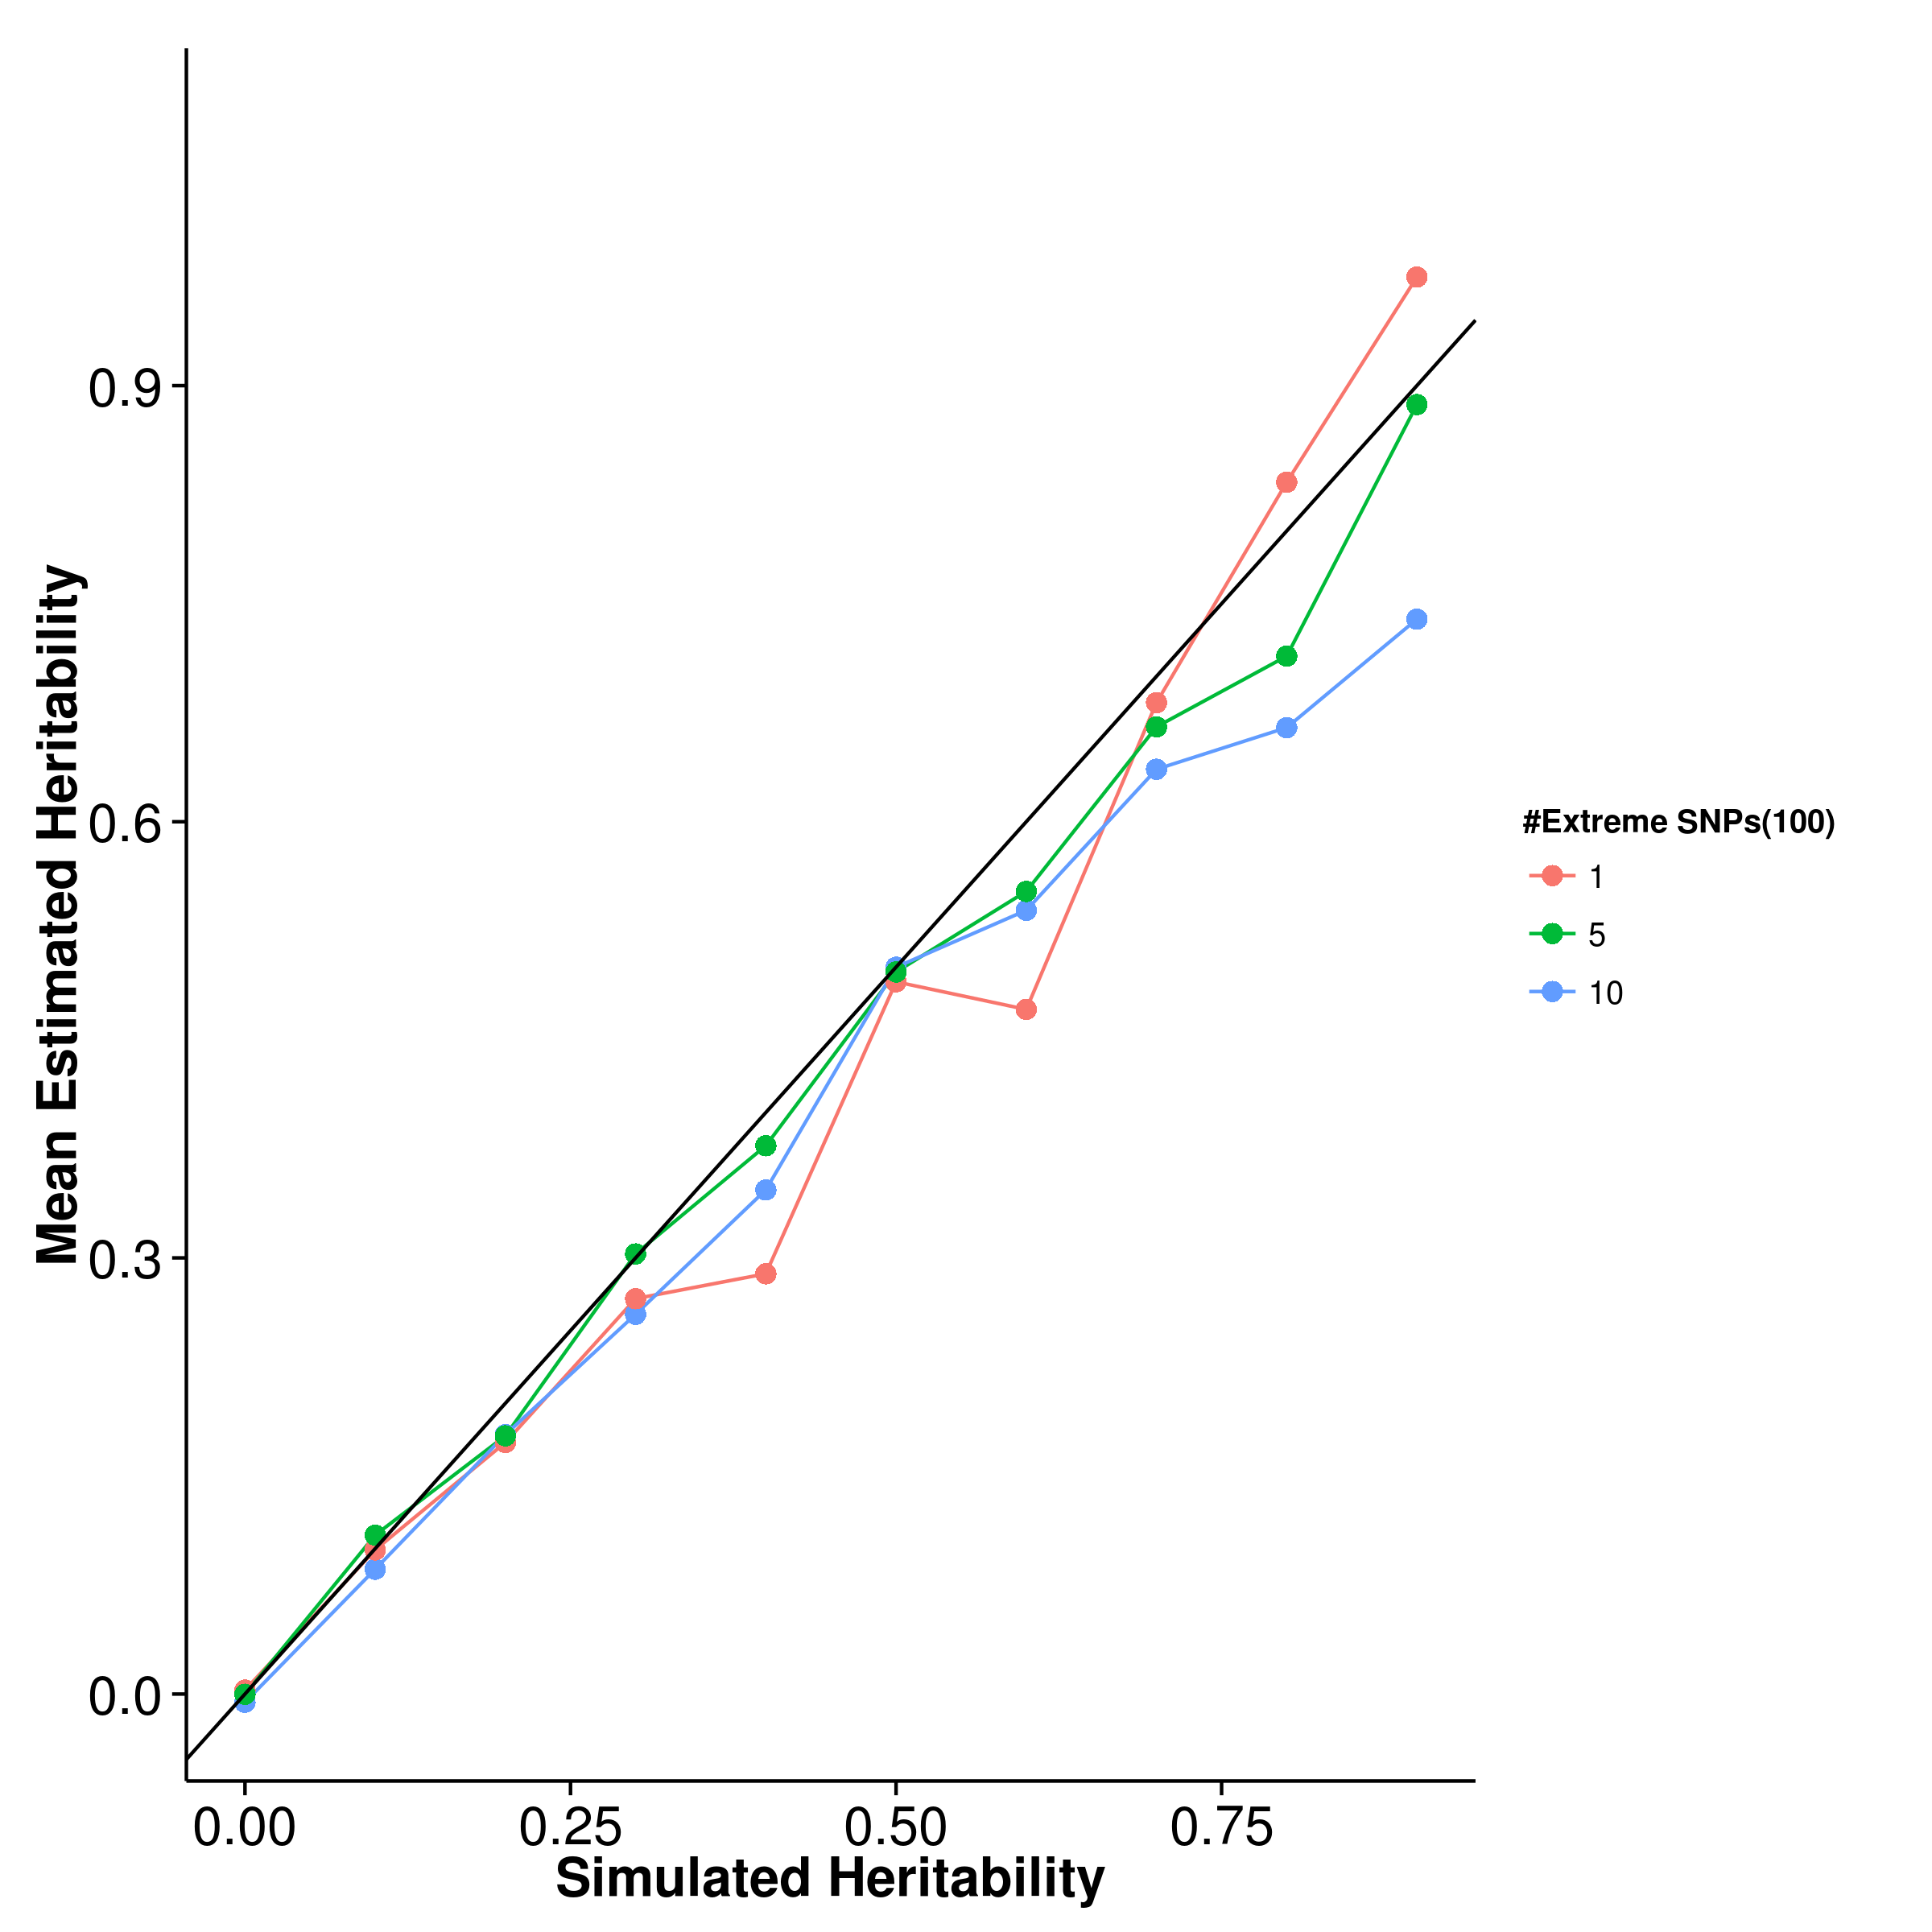
\includegraphics{figure/he_summary/extreme_100c/ldscIn_QtE_Rand_mean.png}}
				\label{fig:ldscInQtEx100cMean}
			}
			\caption[Mean of Extreme Effect Size Simulation Result]
			{Mean of results from quantitative trait simulation with extreme effect size simulation.
				It was observed that the mean estimation of heritability of \gls{shrek} is not affected by the number of \gls{SNP}(s) with large effect but with slight upward bias.
				On the other hand, the mean estimation of \gls{ldsc} and \gls{gcta} seems to fluctuate with respect to the simulated heritability.
				} 
			\label{fig:QtEx100cMean}
		\end{figure}
		
		\begin{figure}
			\centering
			\subfloat[SHREK]{
				\scalebox{.4}{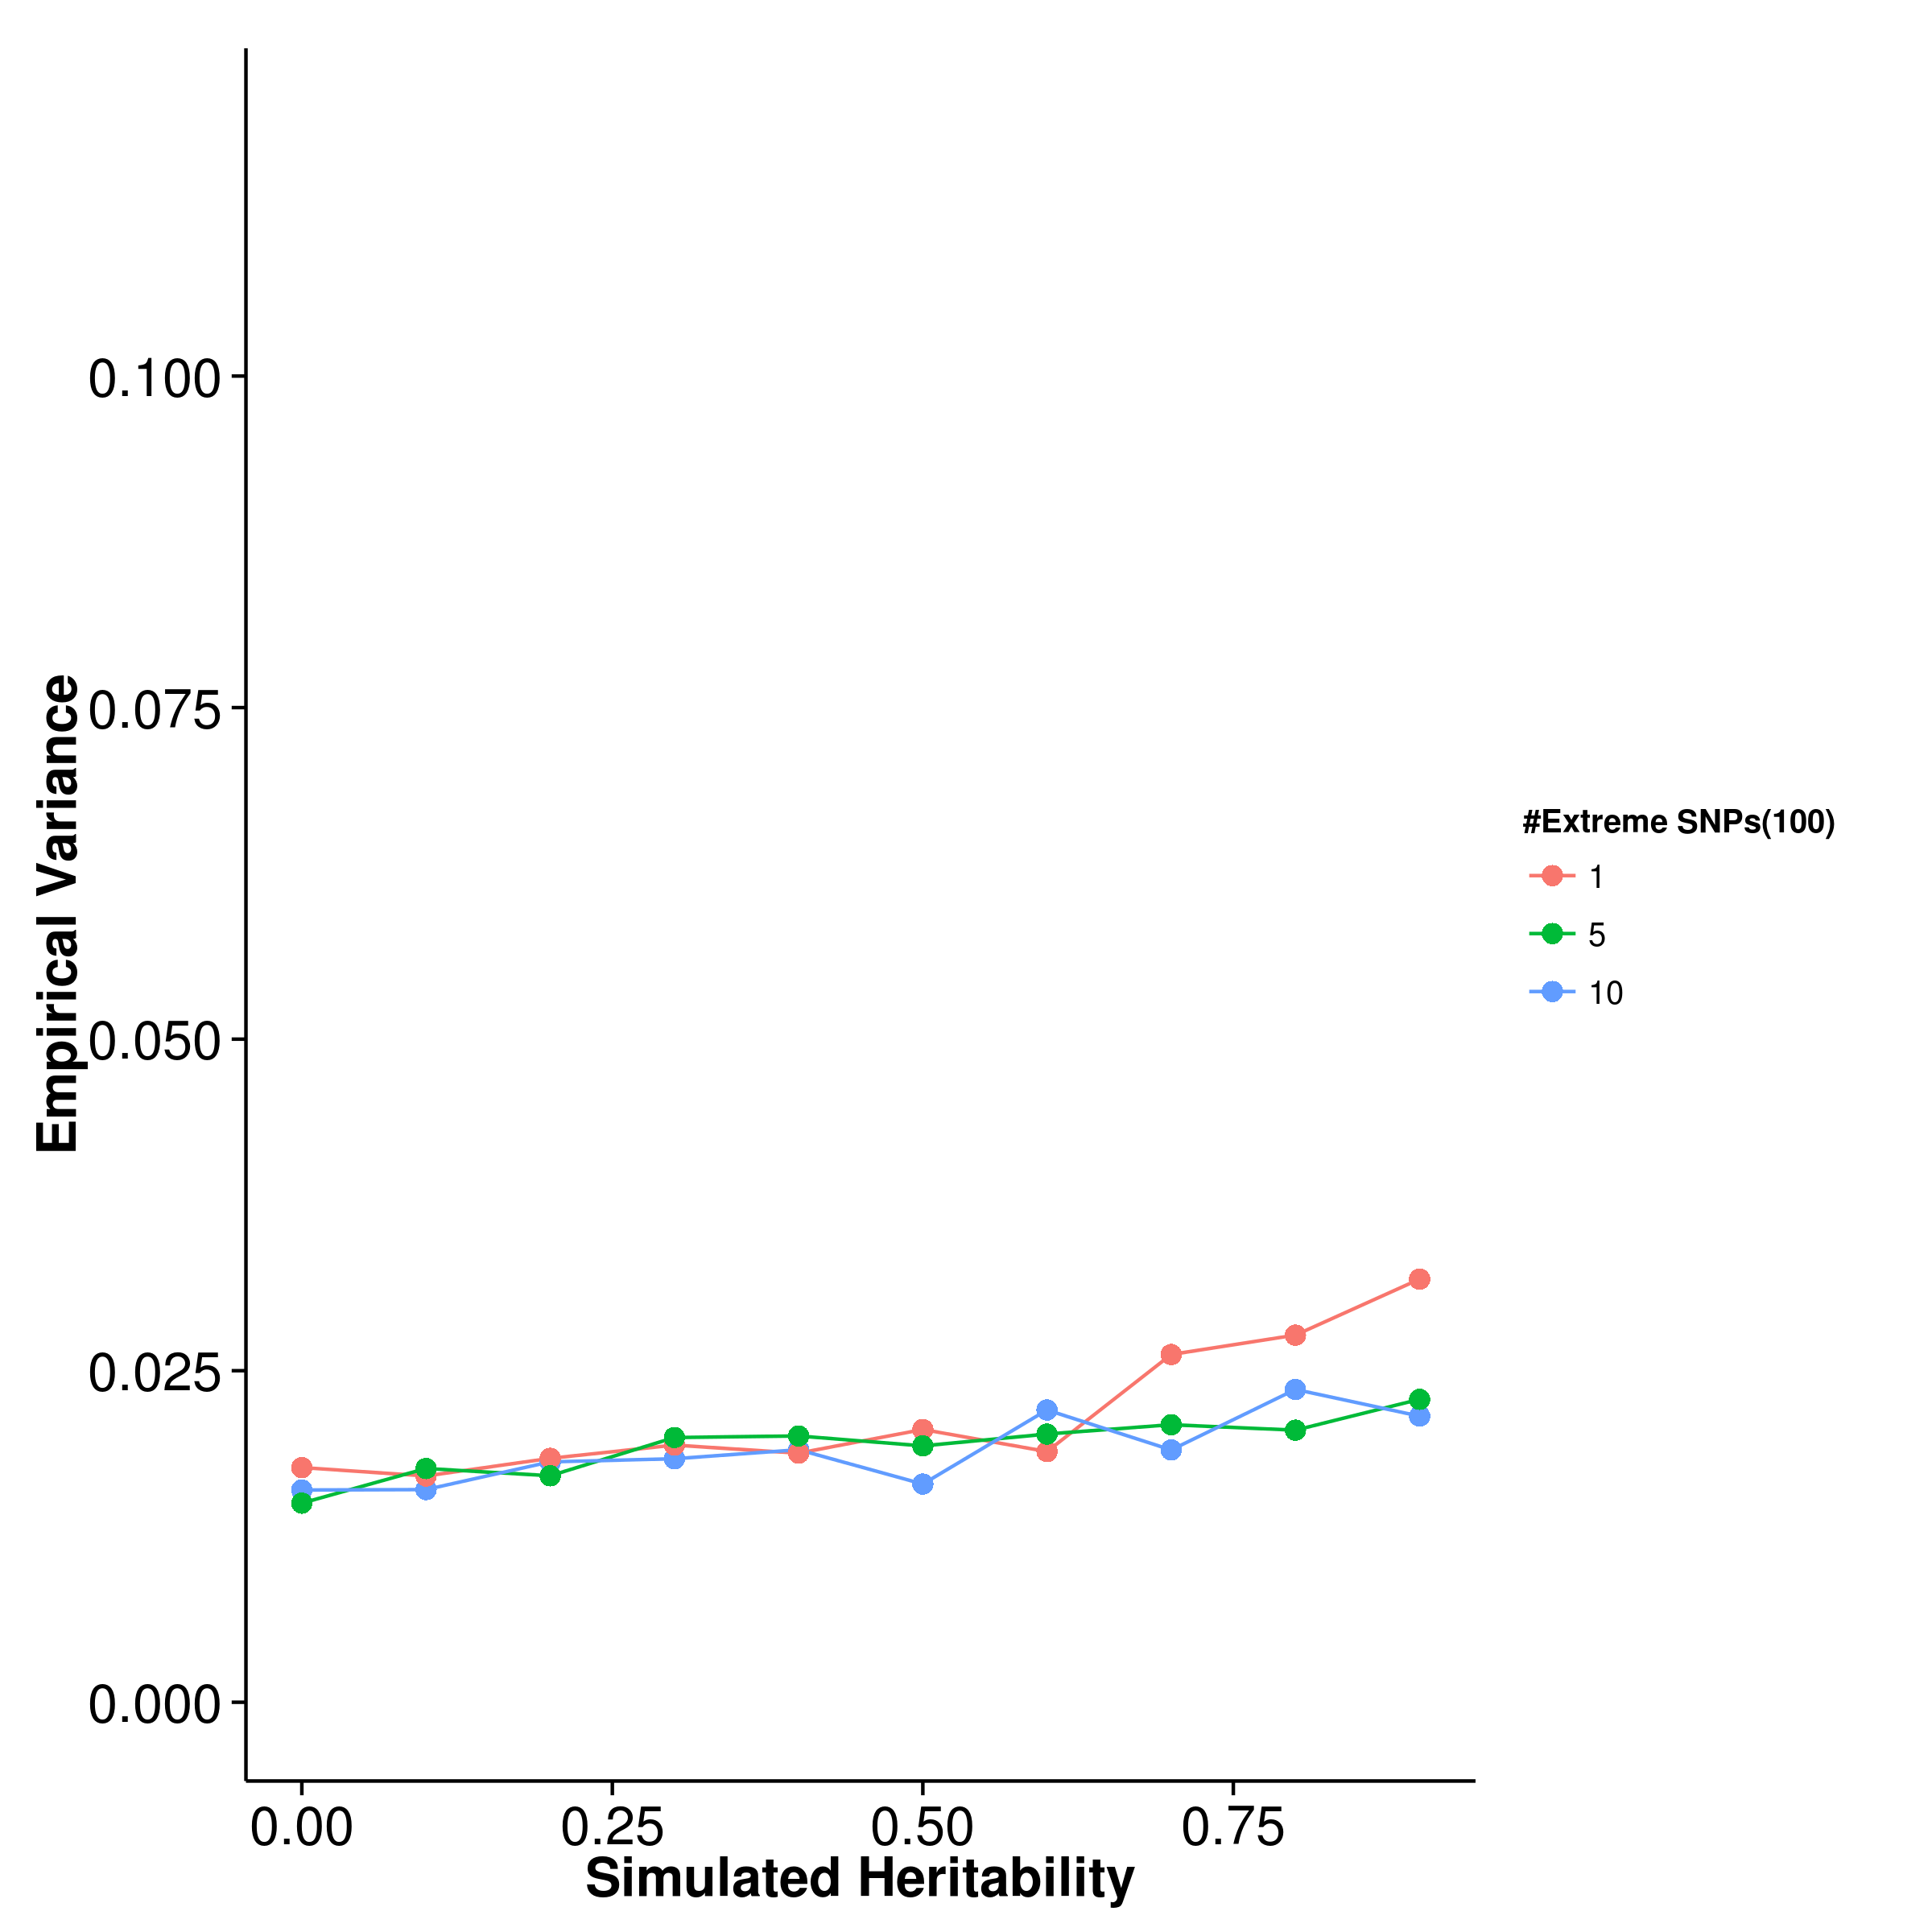
\includegraphics{figure/he_summary/extreme_100c/shrek_QtE_Rand_sd.png}}
				\label{fig:shrekQtEx100cVar}
			}
			\subfloat[GCTA]{
				\scalebox{.4}{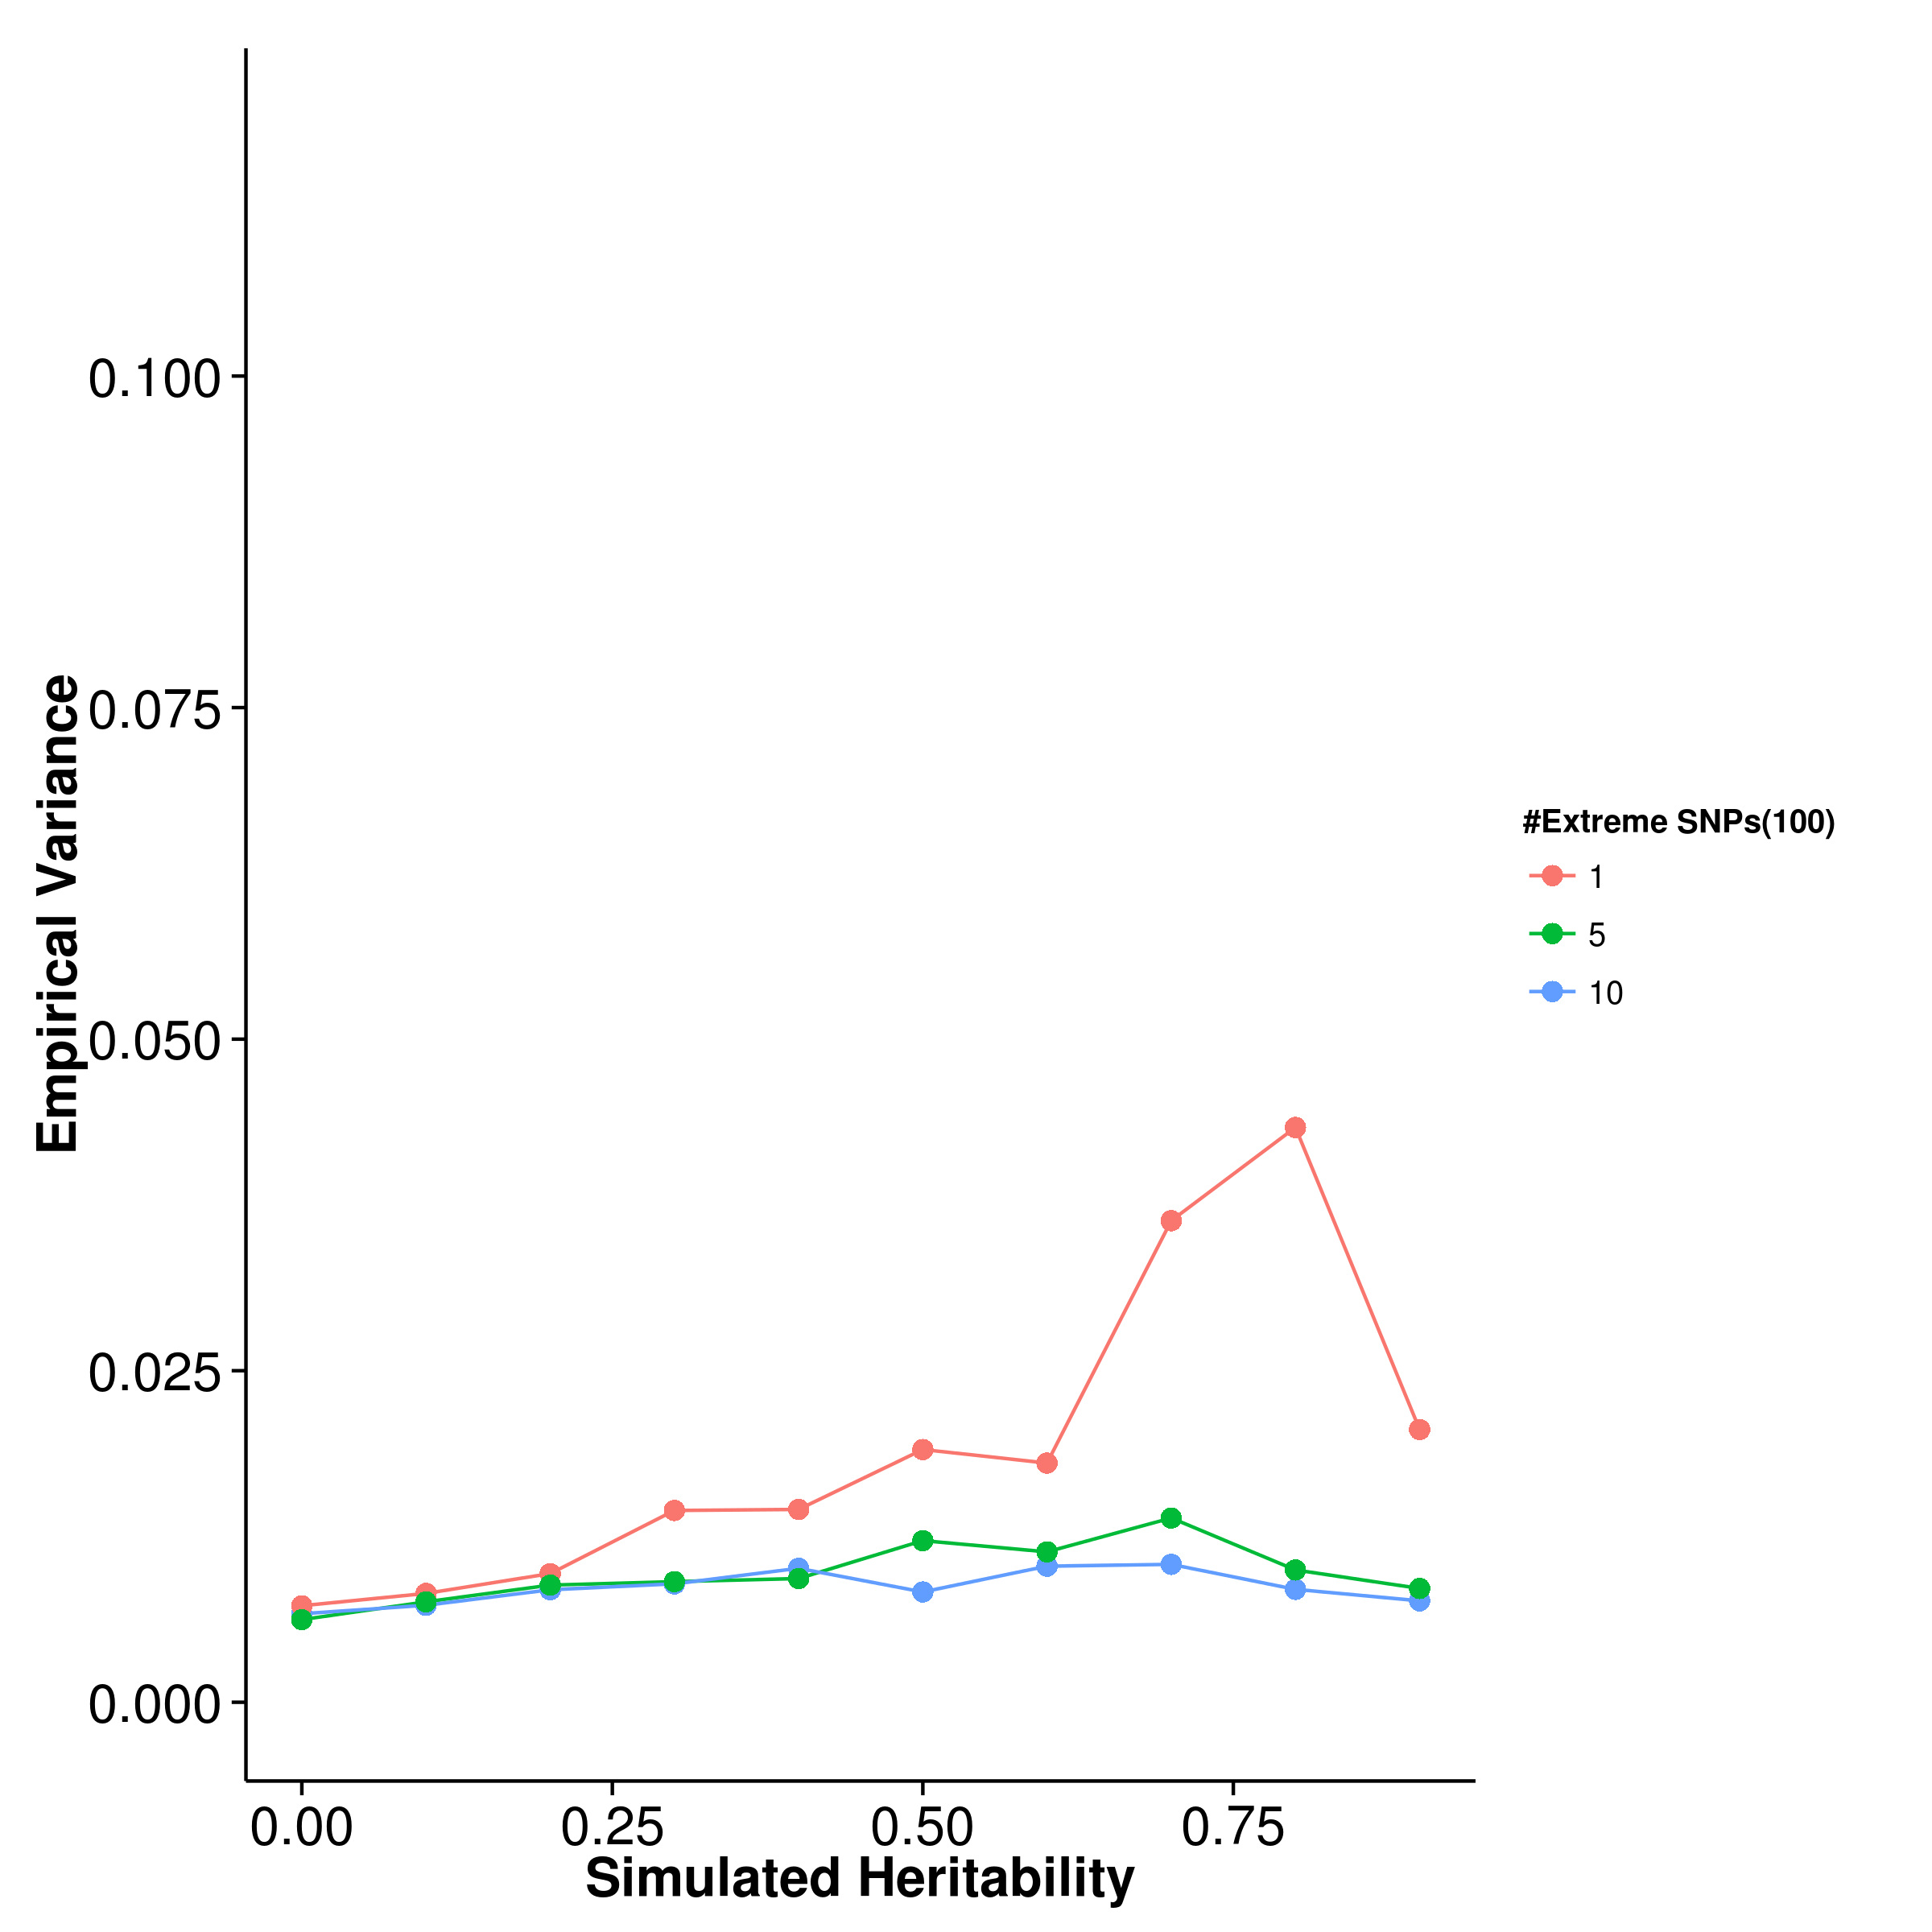
\includegraphics{figure/he_summary/extreme_100c/gcta_QtE_Rand_sd.png}}
				\label{fig:gctaQtEx100cVar}
			}\\
			\subfloat[LDSC with fix intercept]{
				\scalebox{.4}{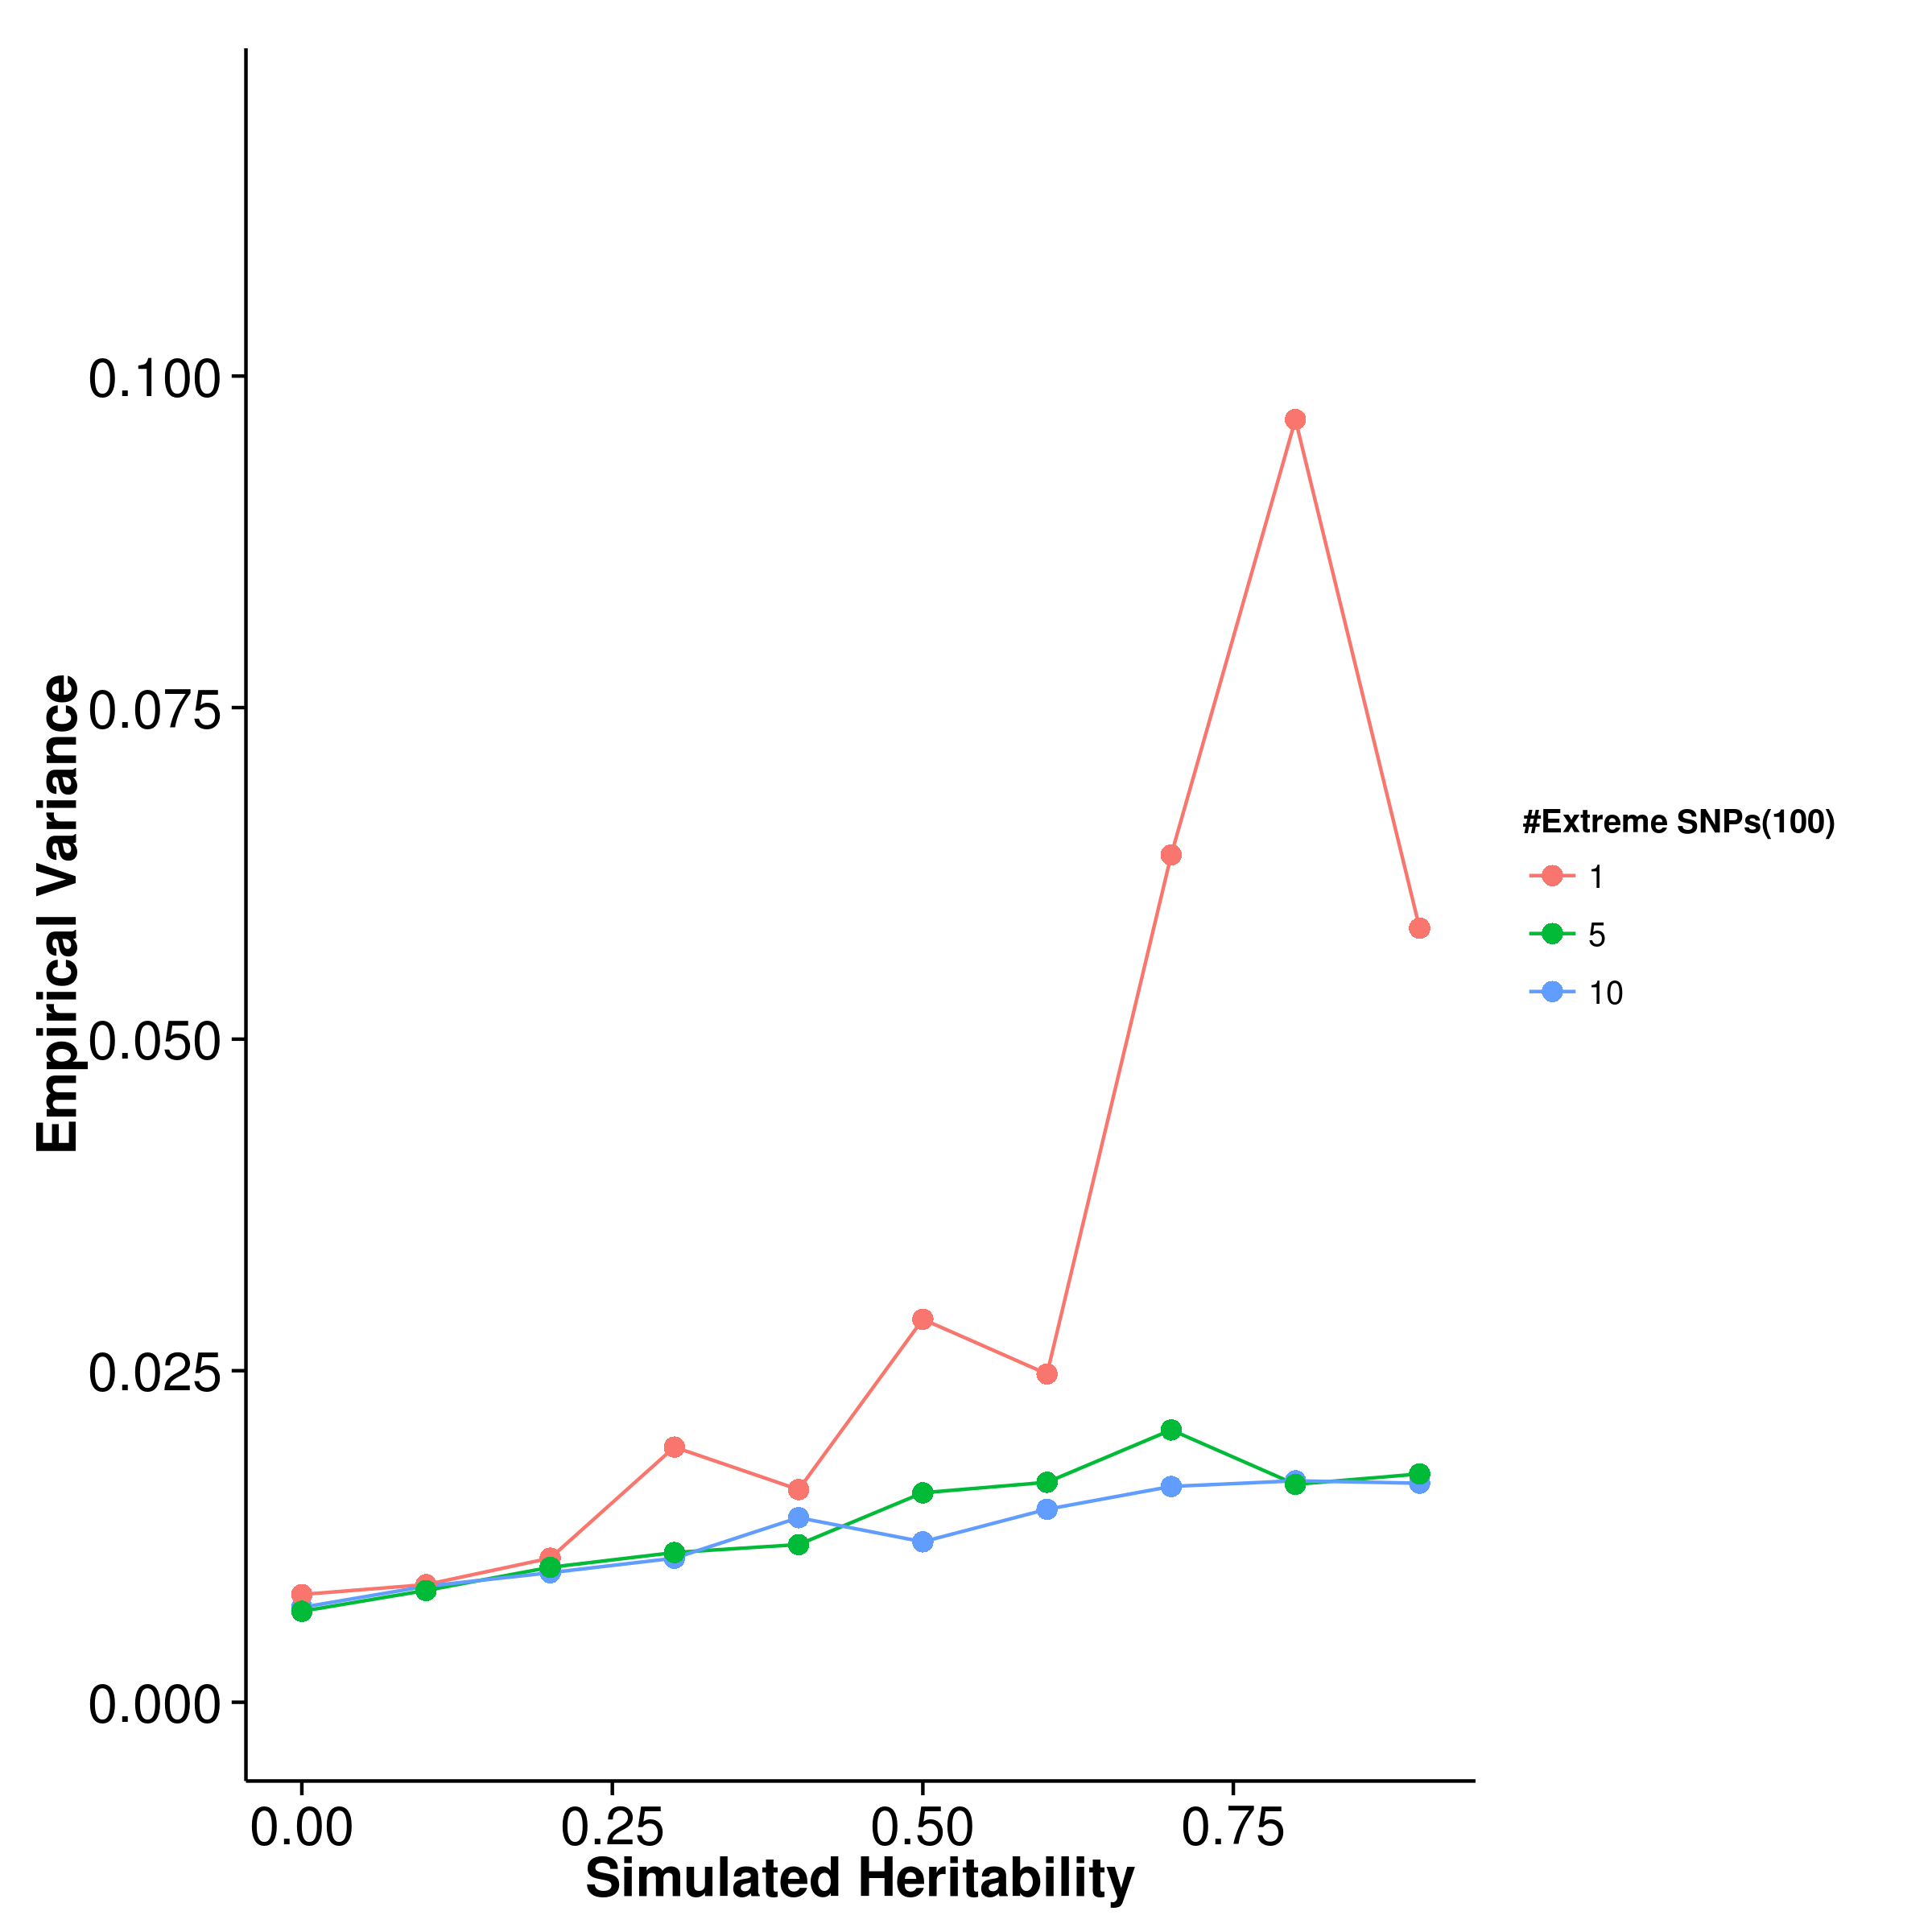
\includegraphics{figure/he_summary/extreme_100c/ldsc_QtE_Rand_sd.png}}
				\label{fig:ldscQtEx100cVar}
			}
			\subfloat[LDSC with intercept estimation]{
				
				\scalebox{.4}{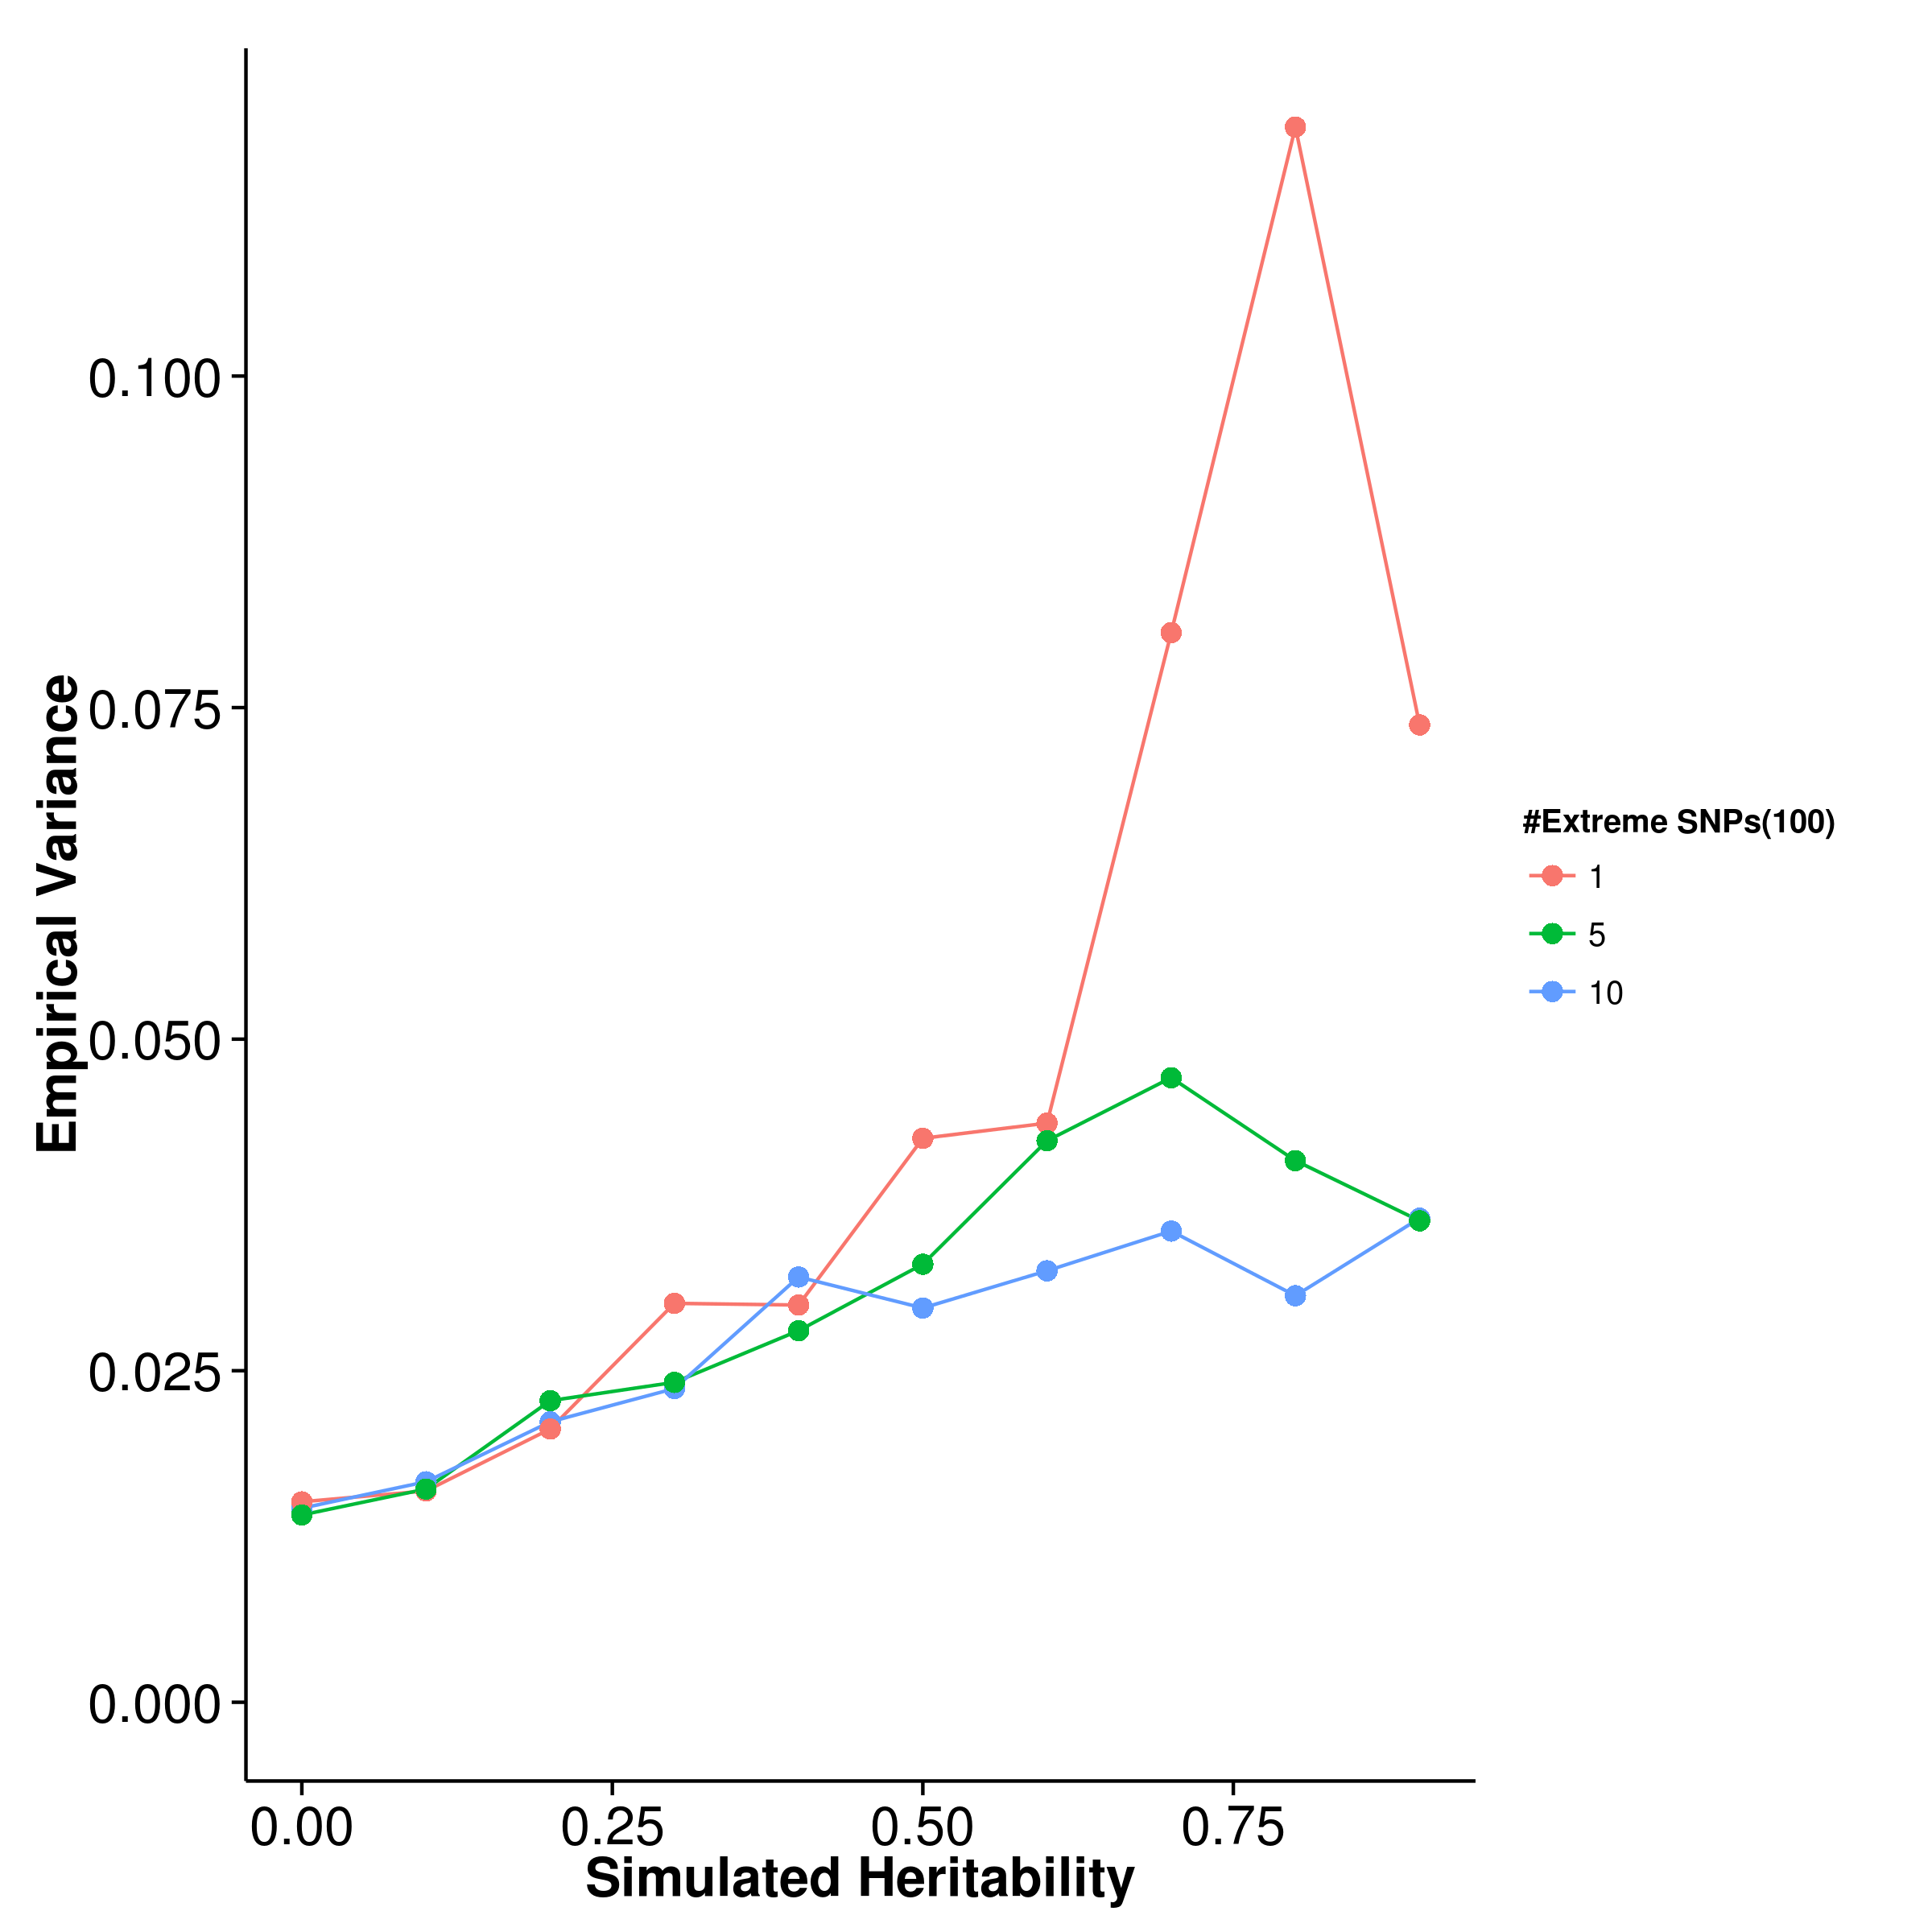
\includegraphics{figure/he_summary/extreme_100c/ldscIn_QtE_Rand_sd.png}}
				\label{fig:ldscInQtEx100cVar}
			}
			\caption[Variance of Extreme Effect Size Simulation Result]
			{Variance of results from quantitative trait simulation with extreme effect size simulation.
				100 causal \glspl{SNP} were simulated.
				When only 1 \gls{SNP} with extreme effect was simulated, the empirical variance of \gls{gcta} and \gls{ldsc} increases and a large fluctuation was observed.
				Whereas the empirical variance of \gls{shrek} only increase slightly when the simulated heritability is large and with only 1 \gls{SNP} with extreme effect.
				Suggesting that it is more robust to the change in number of extreme \gls{SNP}(s).
			} 
			\label{fig:QtEx100cVar}
		\end{figure}
		
		\begin{figure}
			\centering
			\subfloat[SHREK]{
				\scalebox{.4}{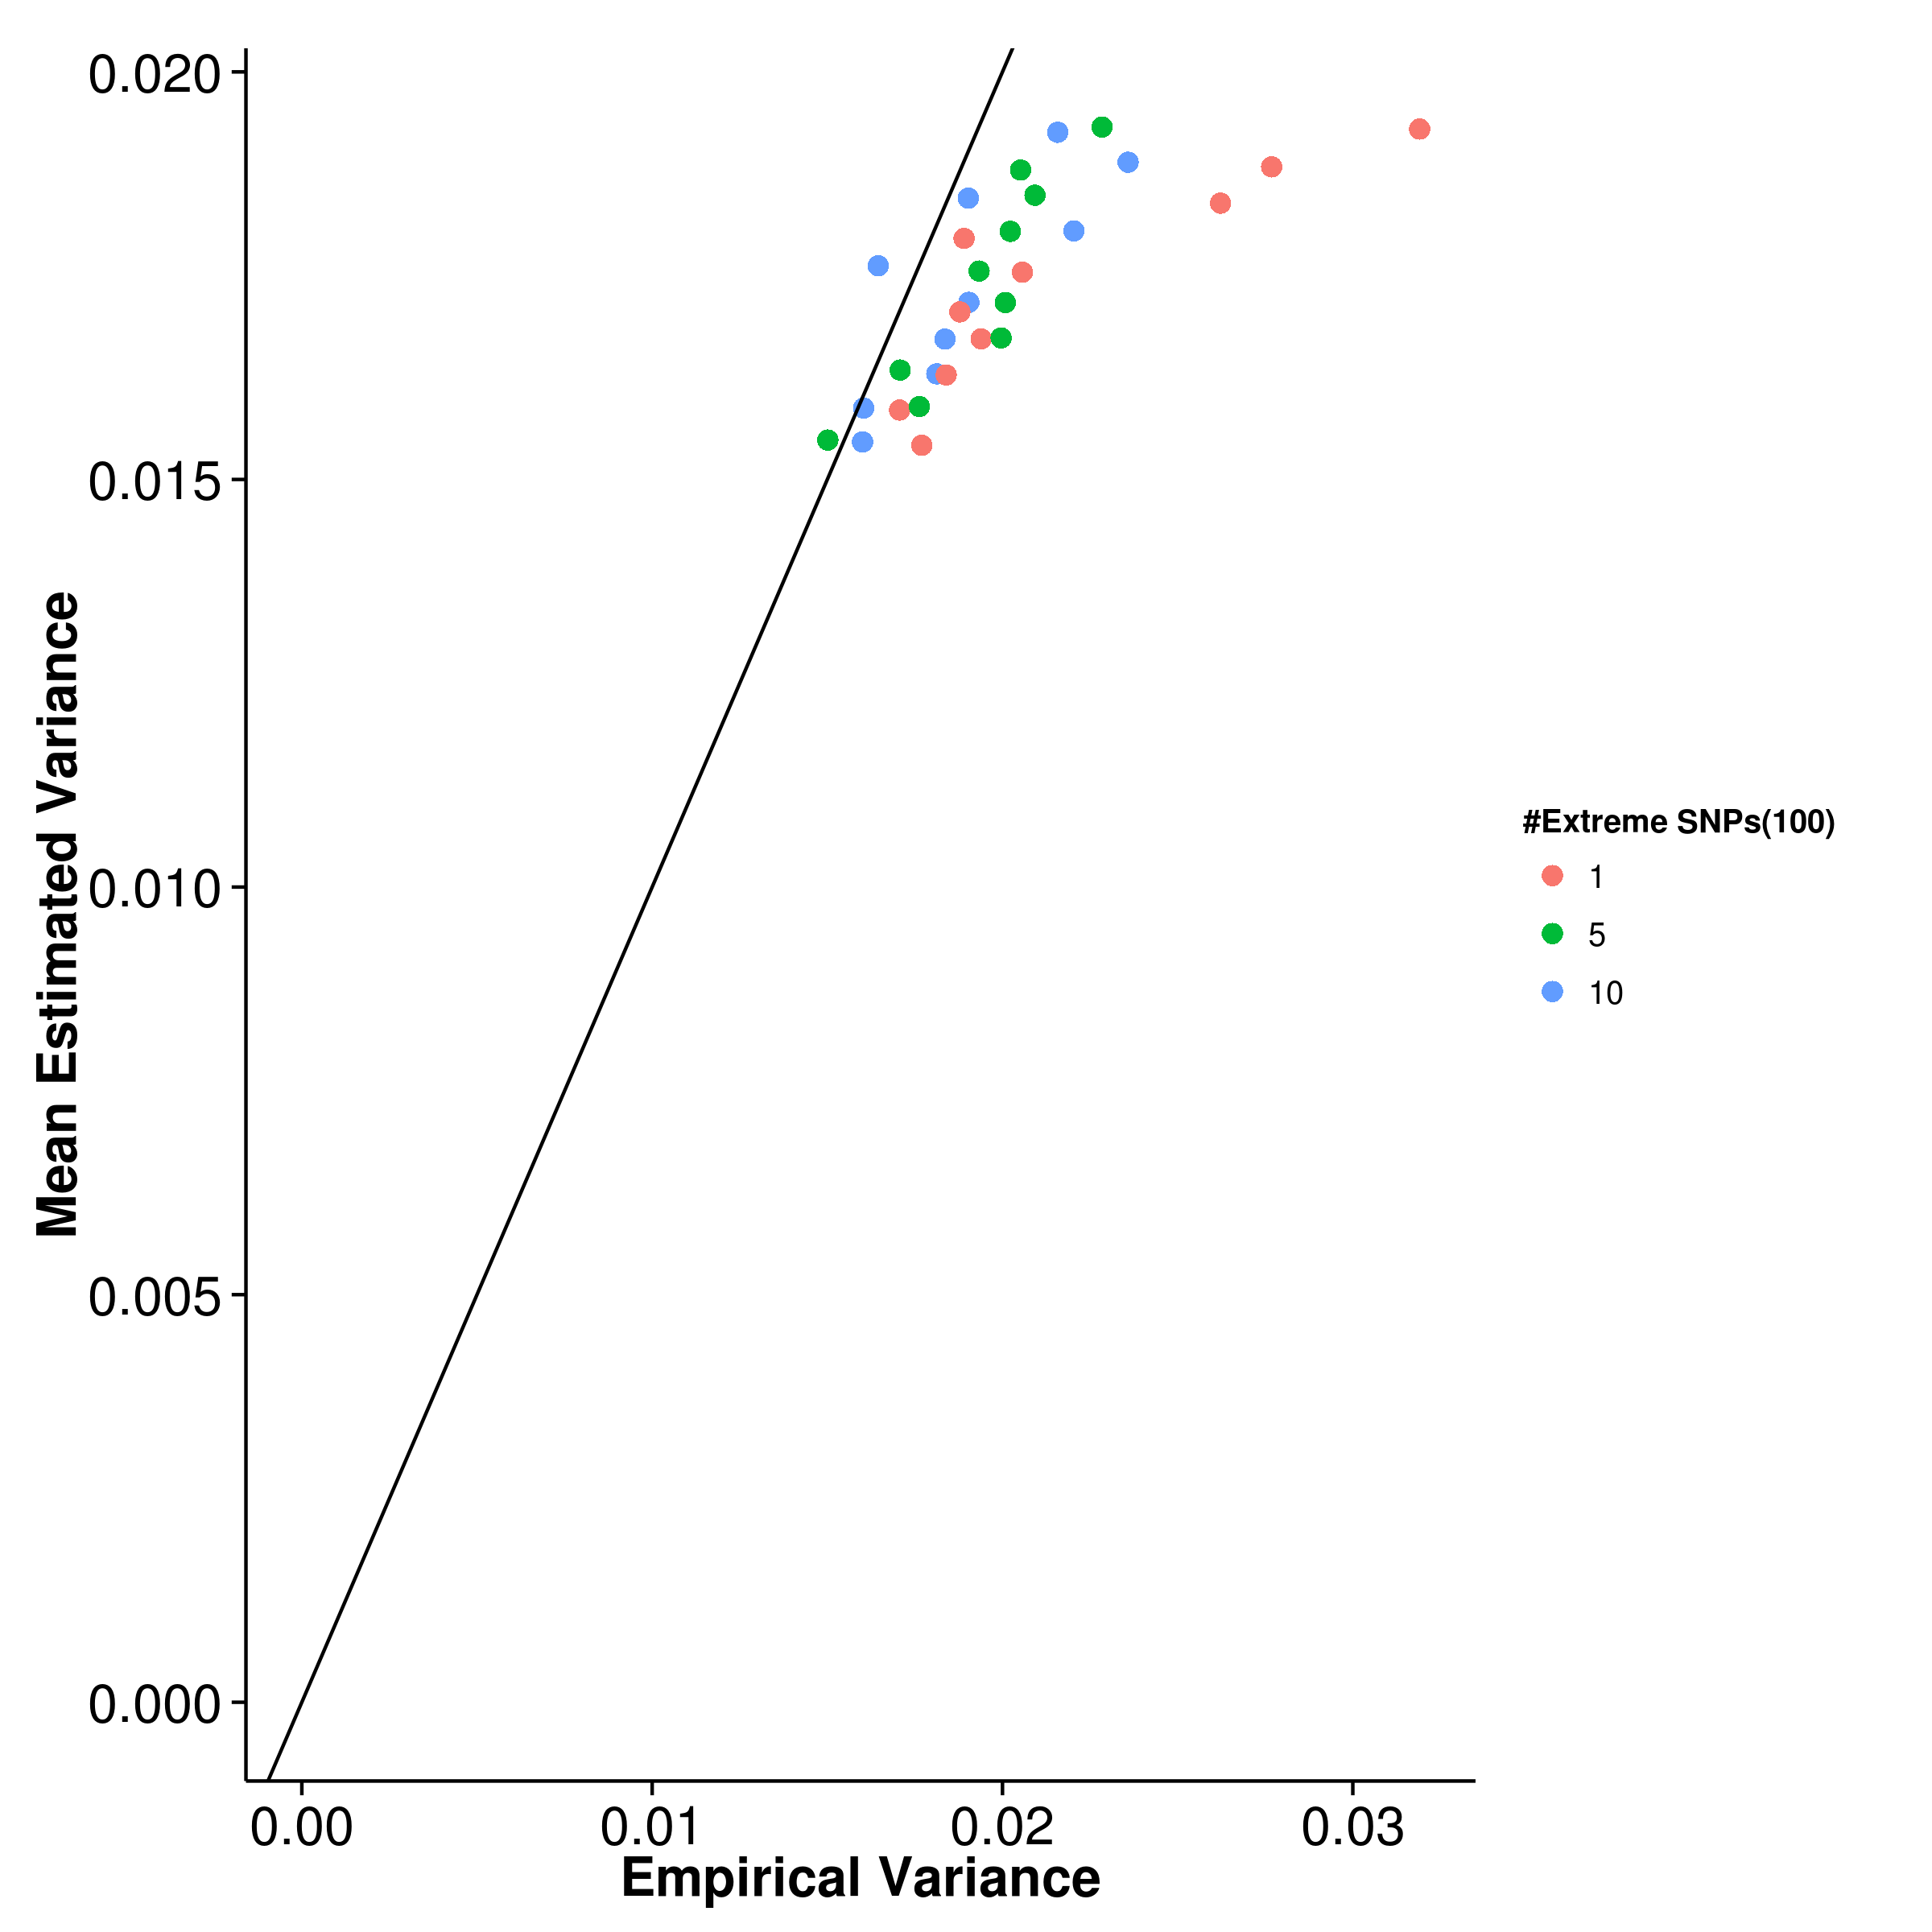
\includegraphics{figure/he_summary/extreme_100c/shrek_QtE_Rand_sdCom.png}}
				\label{fig:shrekQtEx100cVarCom}
			}
			\subfloat[GCTA]{
				\scalebox{.4}{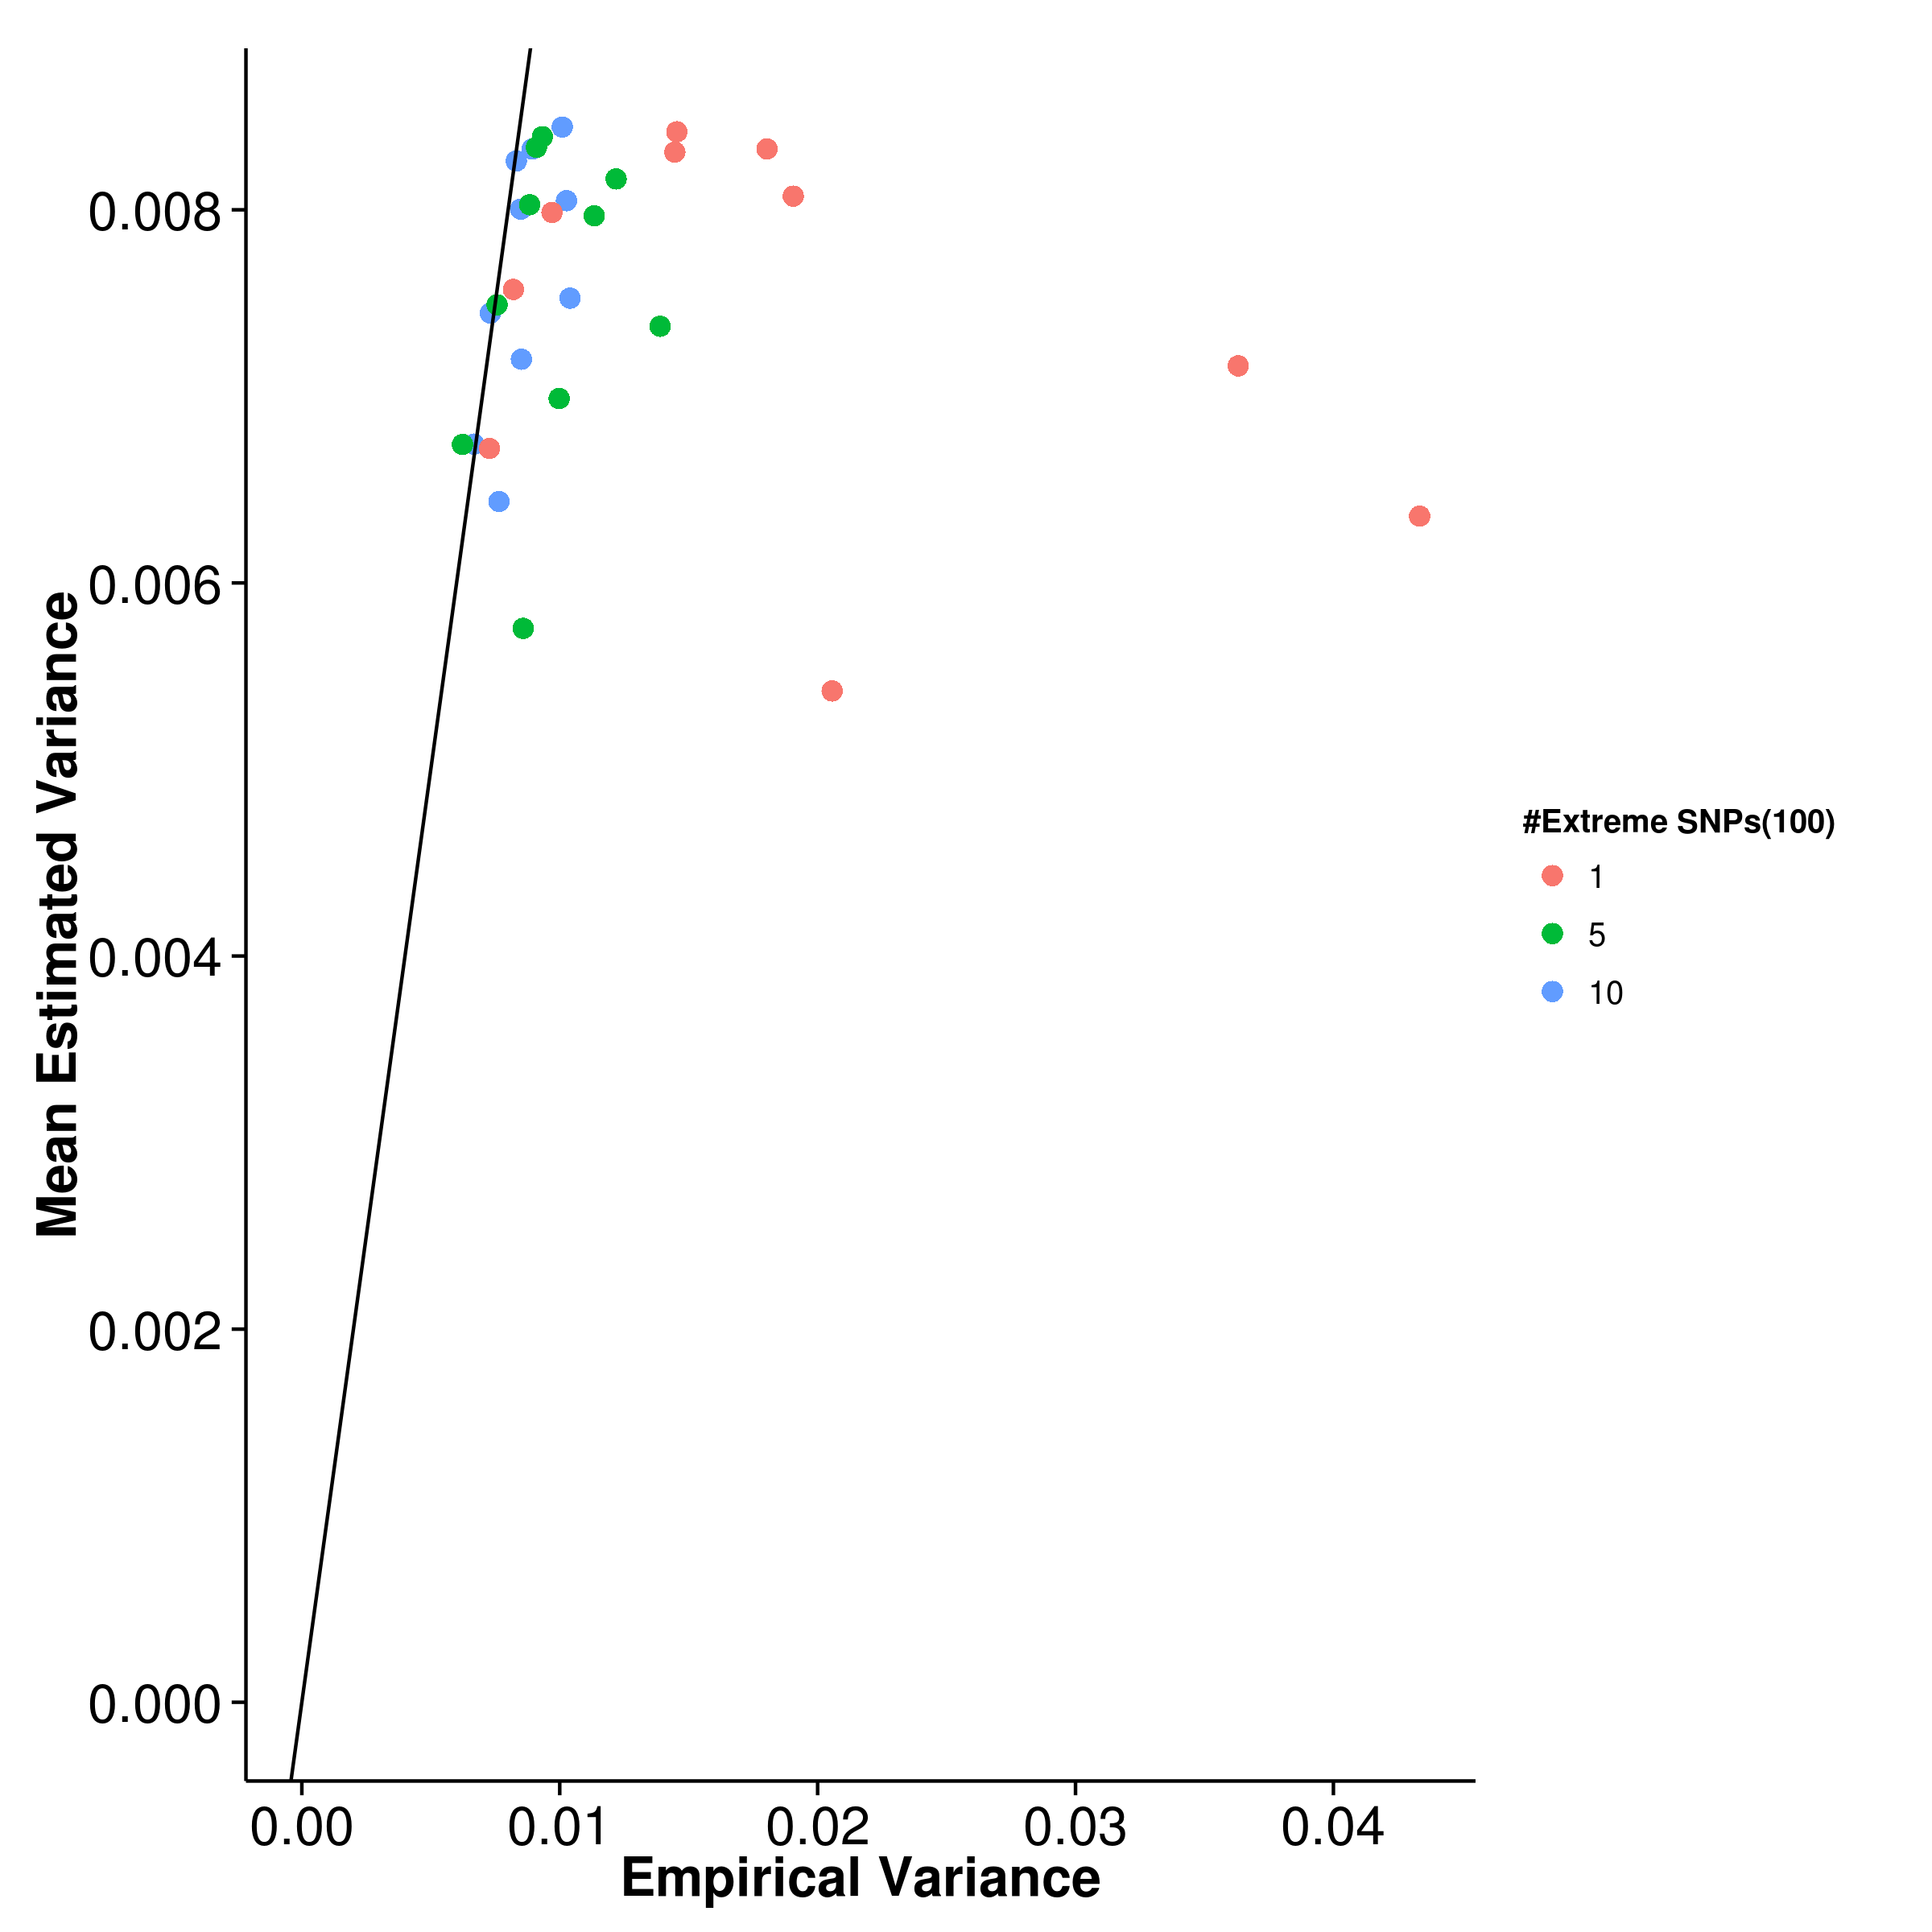
\includegraphics{figure/he_summary/extreme_100c/gcta_QtE_Rand_sdCom.png}}
				\label{fig:gctaQtEx100cVarCom}
			}\\
			\subfloat[LDSC with fix intercept]{
				\scalebox{.4}{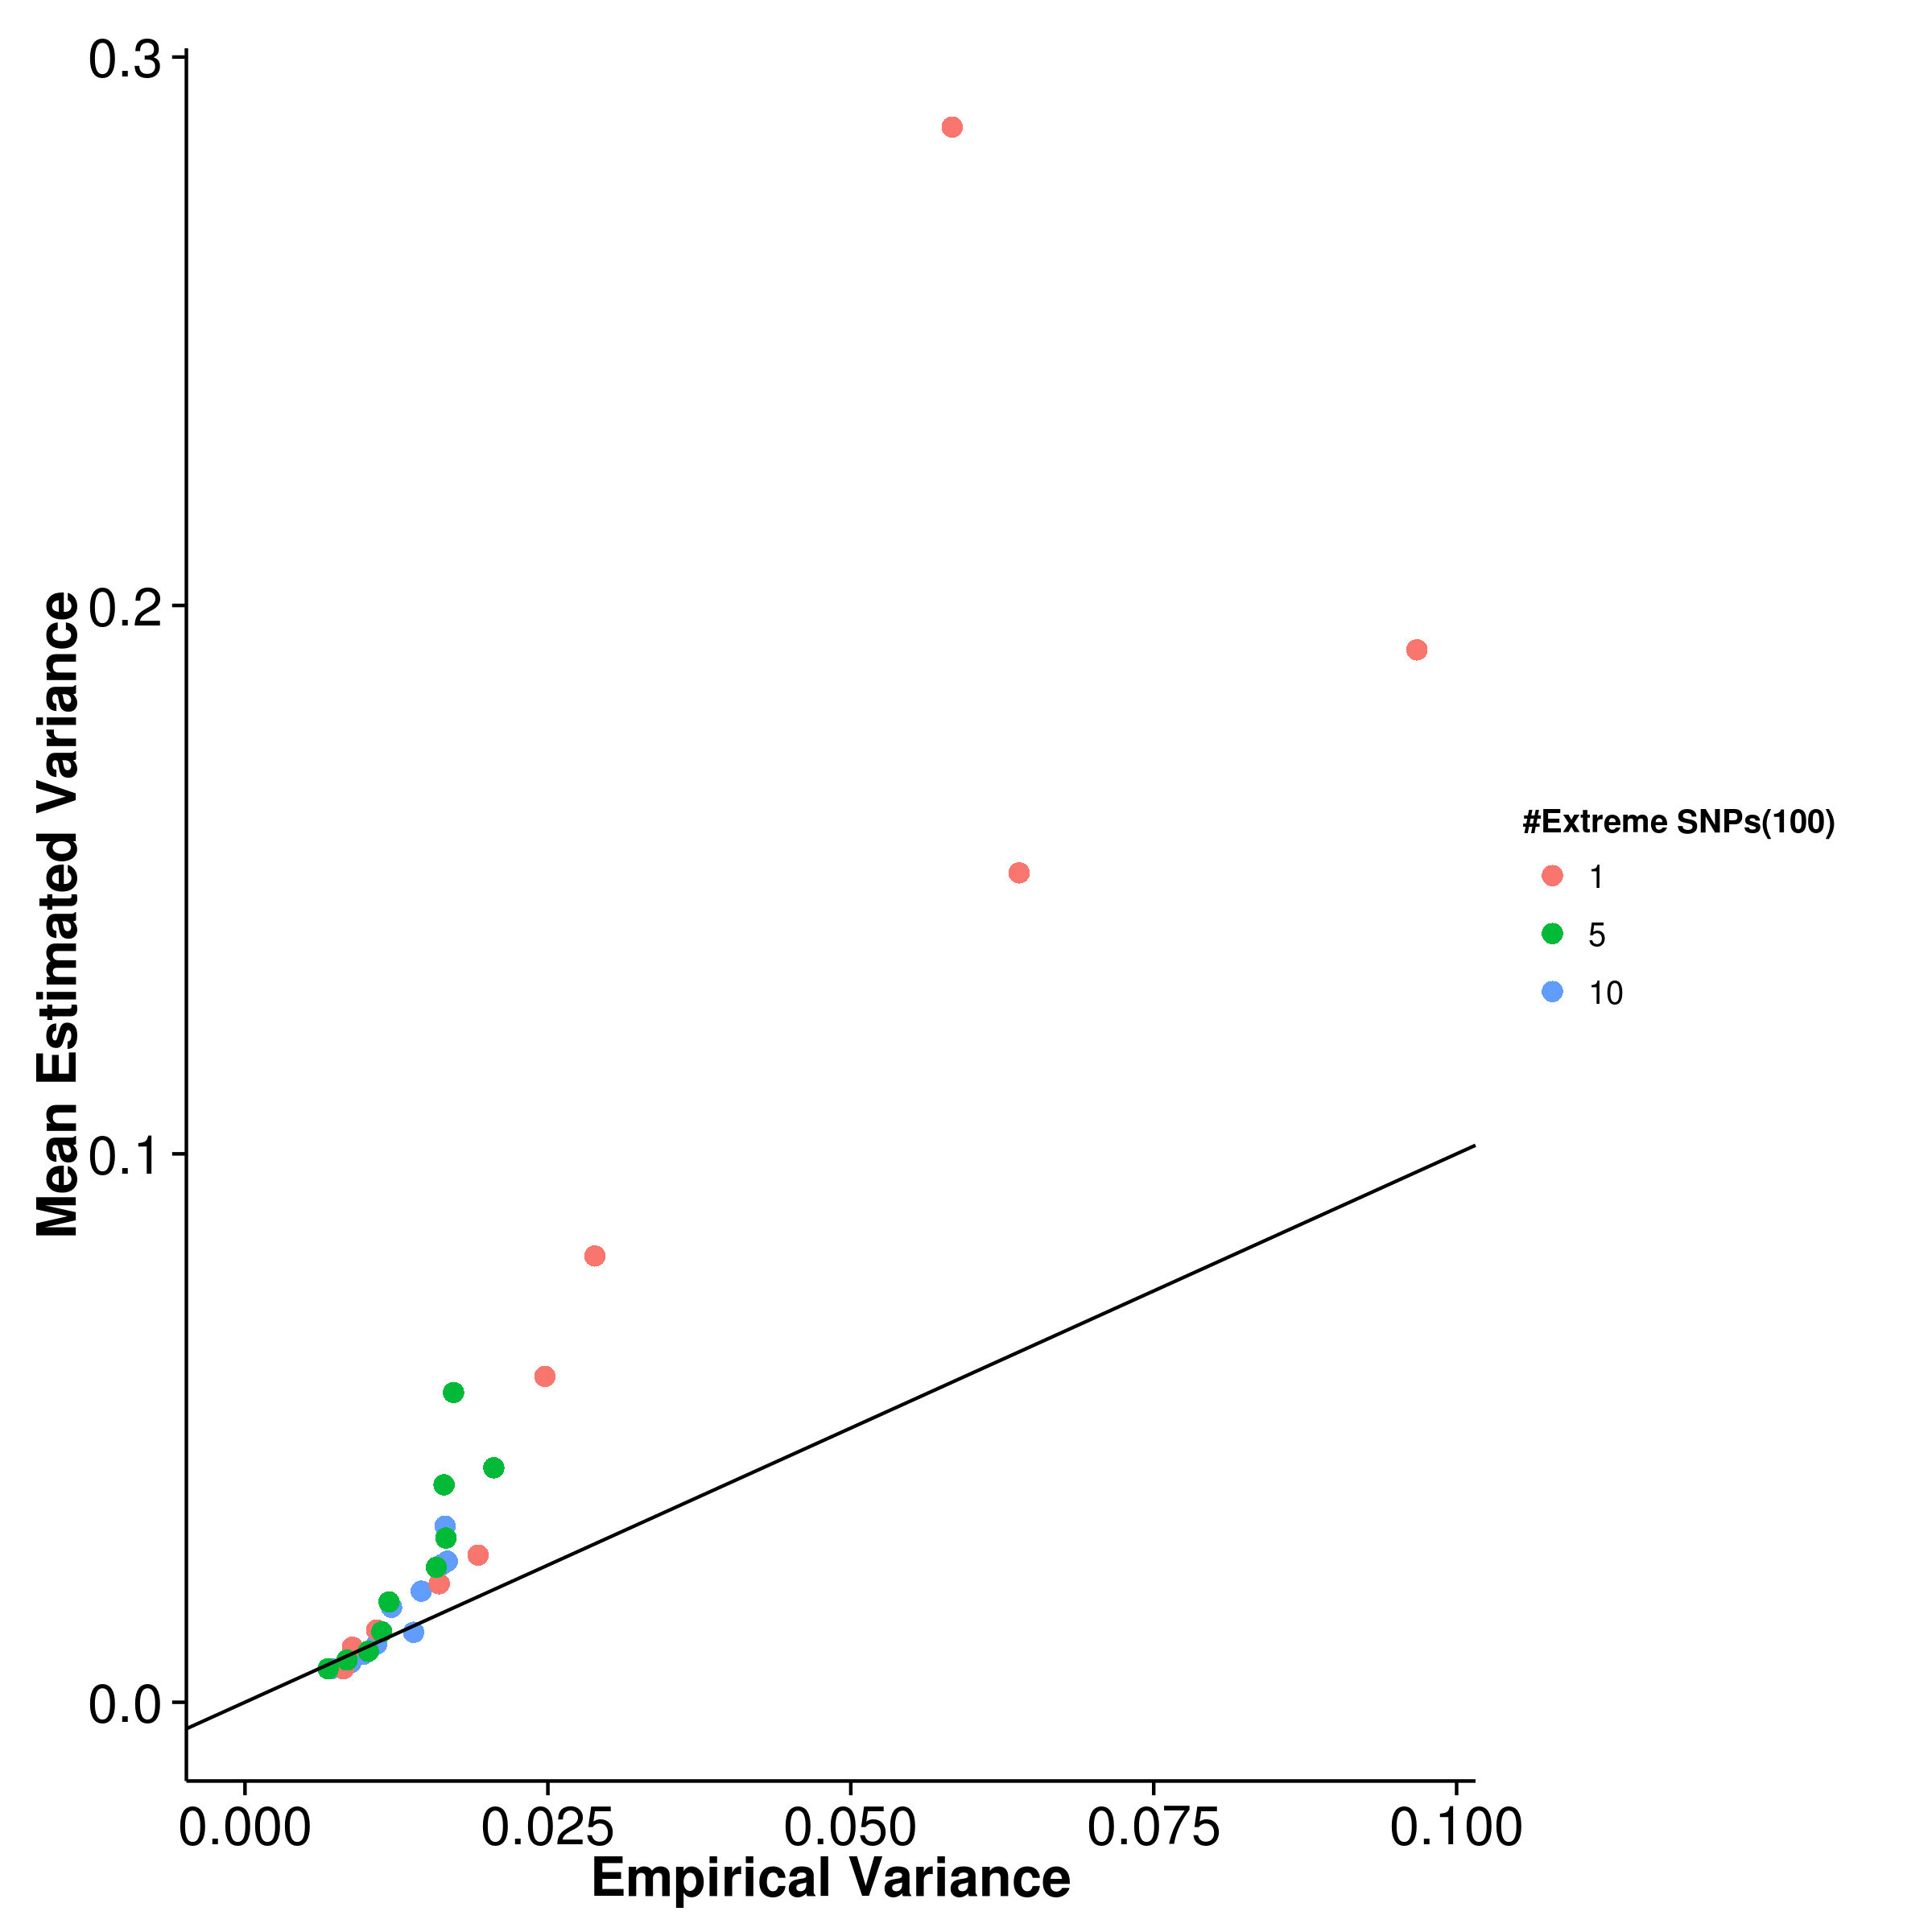
\includegraphics{figure/he_summary/extreme_100c/ldsc_QtE_Rand_sdCom.png}}
				\label{fig:ldscQtEx100cVarCom}
			}
			\subfloat[LDSC with intercept estimation]{
				
				\scalebox{.4}{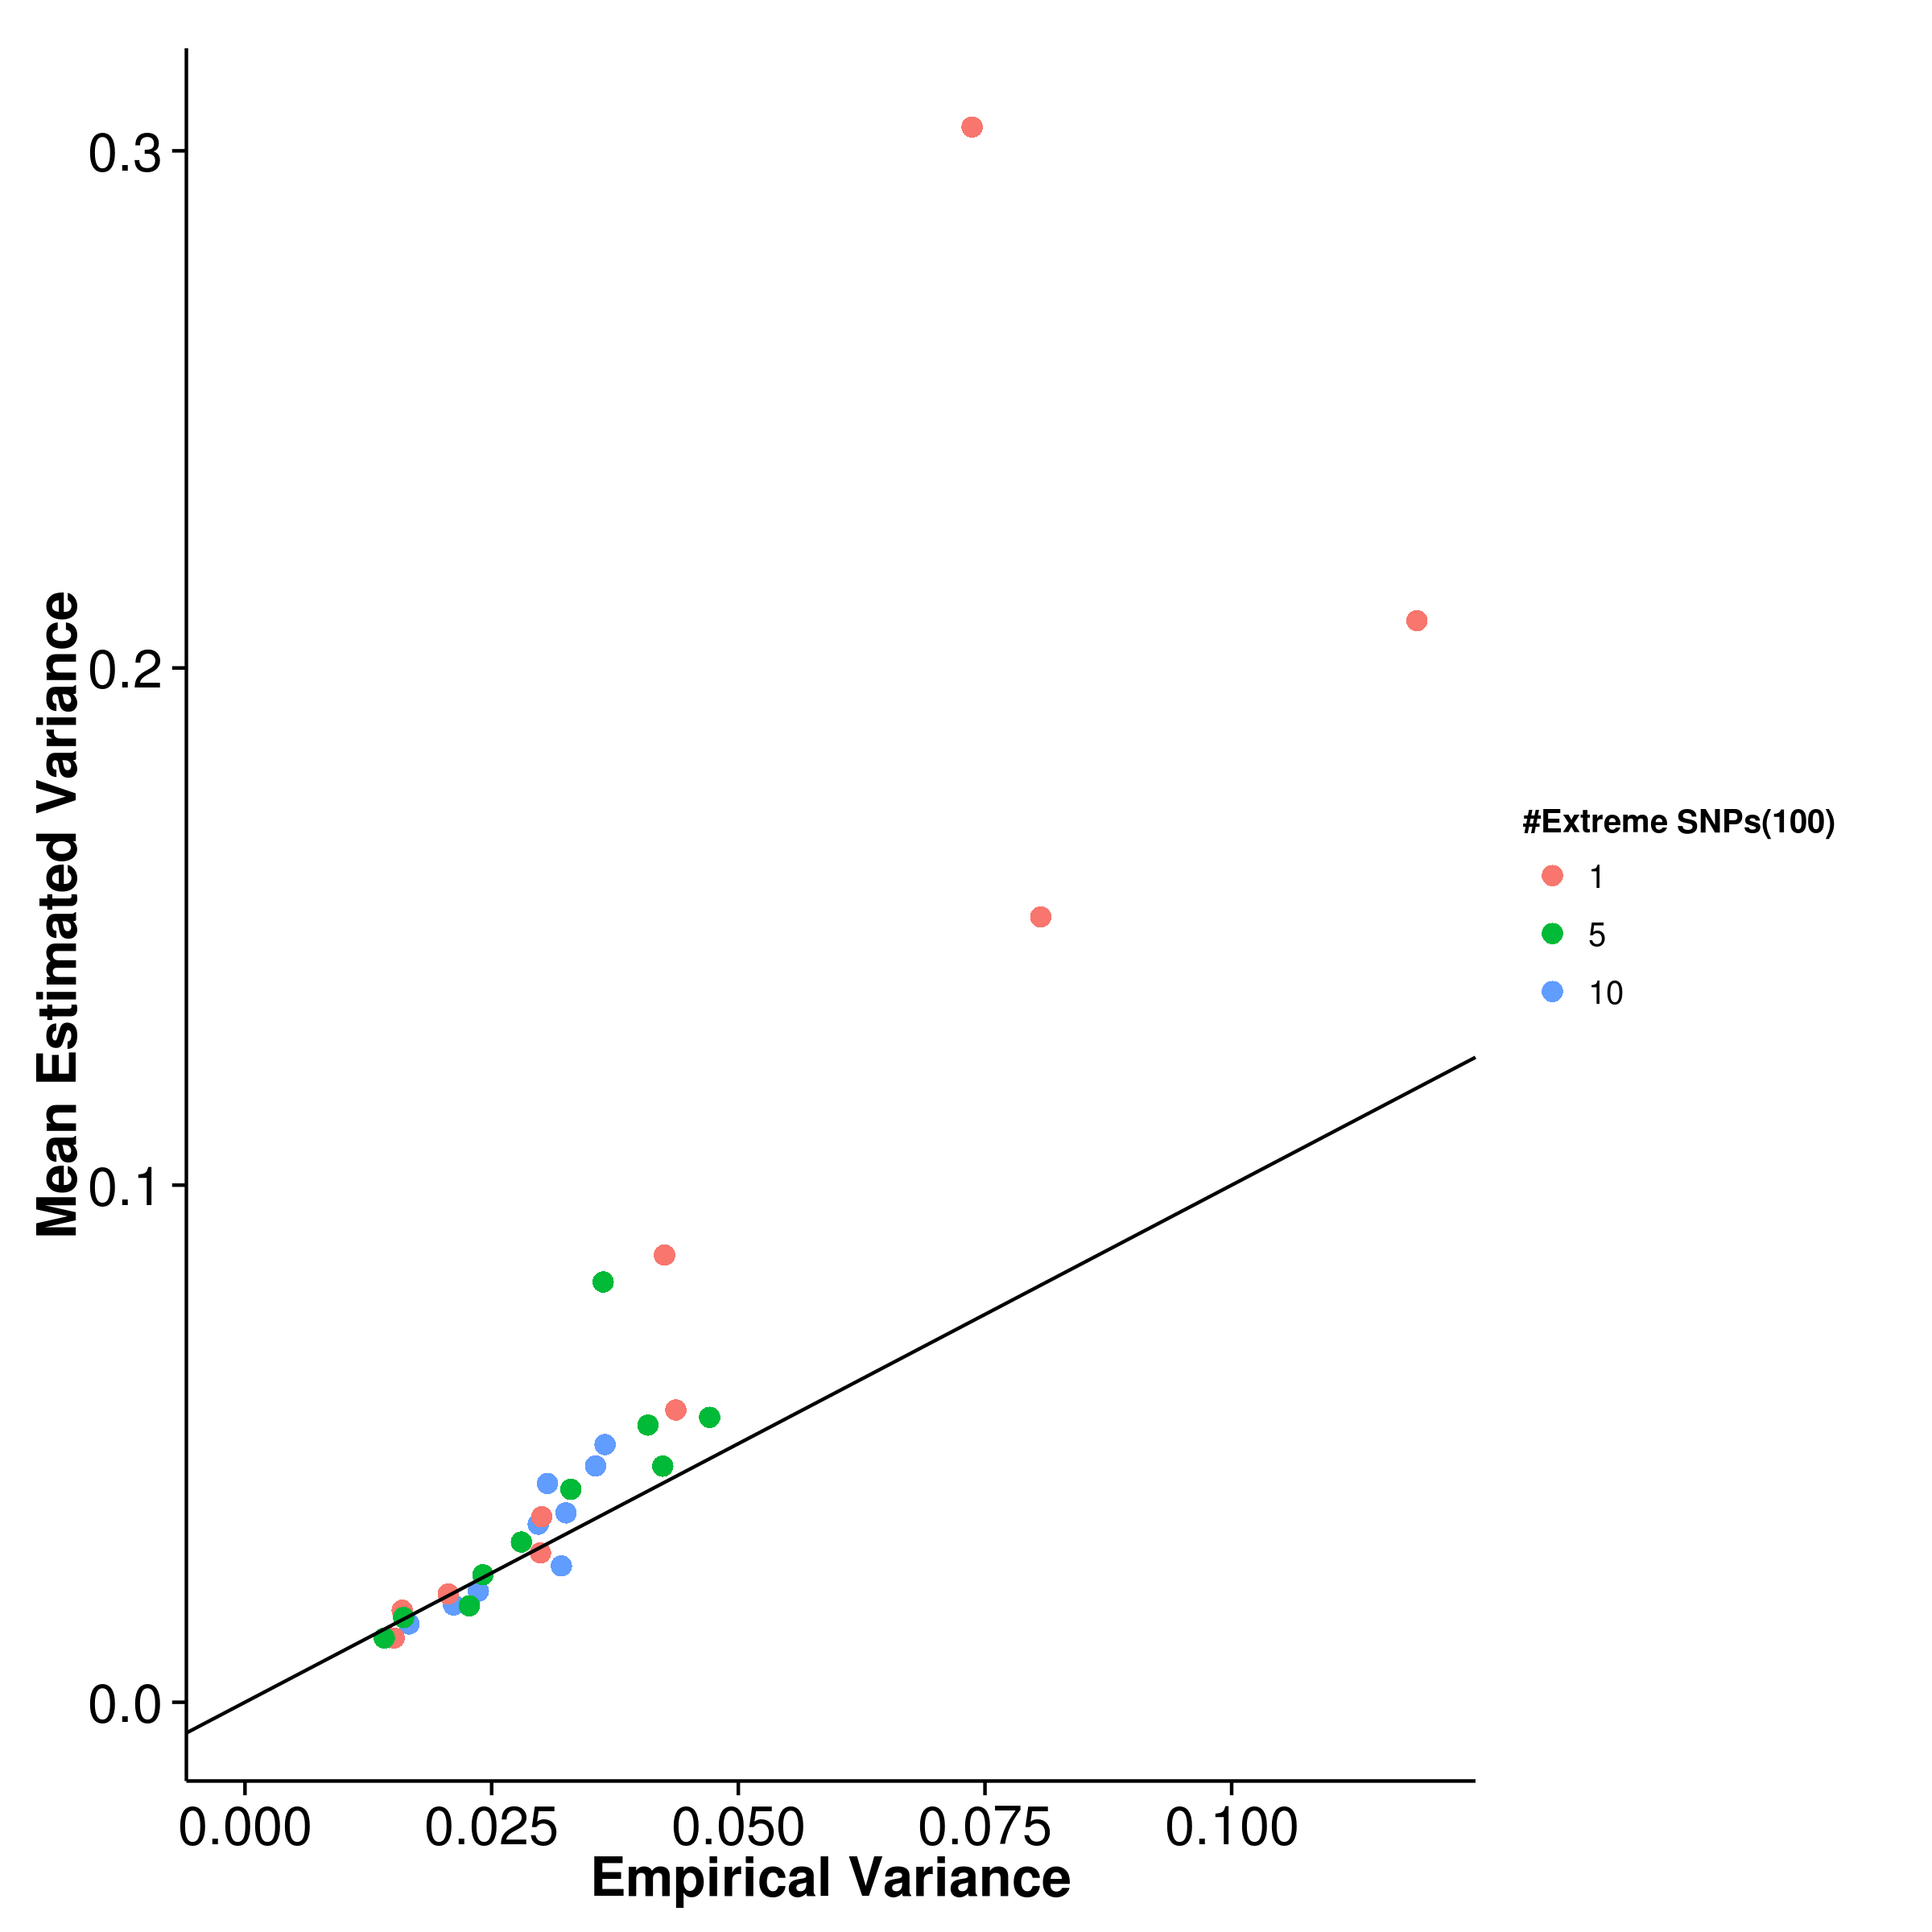
\includegraphics{figure/he_summary/extreme_100c/ldscIn_QtE_Rand_sdCom.png}}
				\label{fig:ldscInQtEx100cVarCom}
			}
			\caption[Estimation of Variance in Extreme Effect Size Simulation]
			{Estimated variance of results from quantitative trait simulation with extreme effect size simulation when compared to the empirical variance.
				100 causal \glspl{SNP} were simulated.
				\gls{shrek} and \gls{gcta} generally under-estimate the variance with the magnitude of bias being the highest when there is only 1 \gls{SNP} with extreme effect.
				On the other hand, \gls{ldsc} tends to over-estimate the variance and it can overestimate the variance by more than 3 folds when there is only 1 \gls{SNP} with extreme effect.
			} 
			\label{fig:QtEx100cVarCom}
		\end{figure}
		Another condition that we were interested in was in the case where a small portion of \glspl{SNP} has a much larger effect than other \glspl{SNP}.
		In this simulation, we simulated either 100 or 250 causal \glspl{SNP} with 1, 5 or 10 \glspl{SNP} having a much larger effect.
		
		% Extreme with 250 causal
		
		\begin{figure}
			\centering
			\subfloat[SHREK]{
				\scalebox{.4}{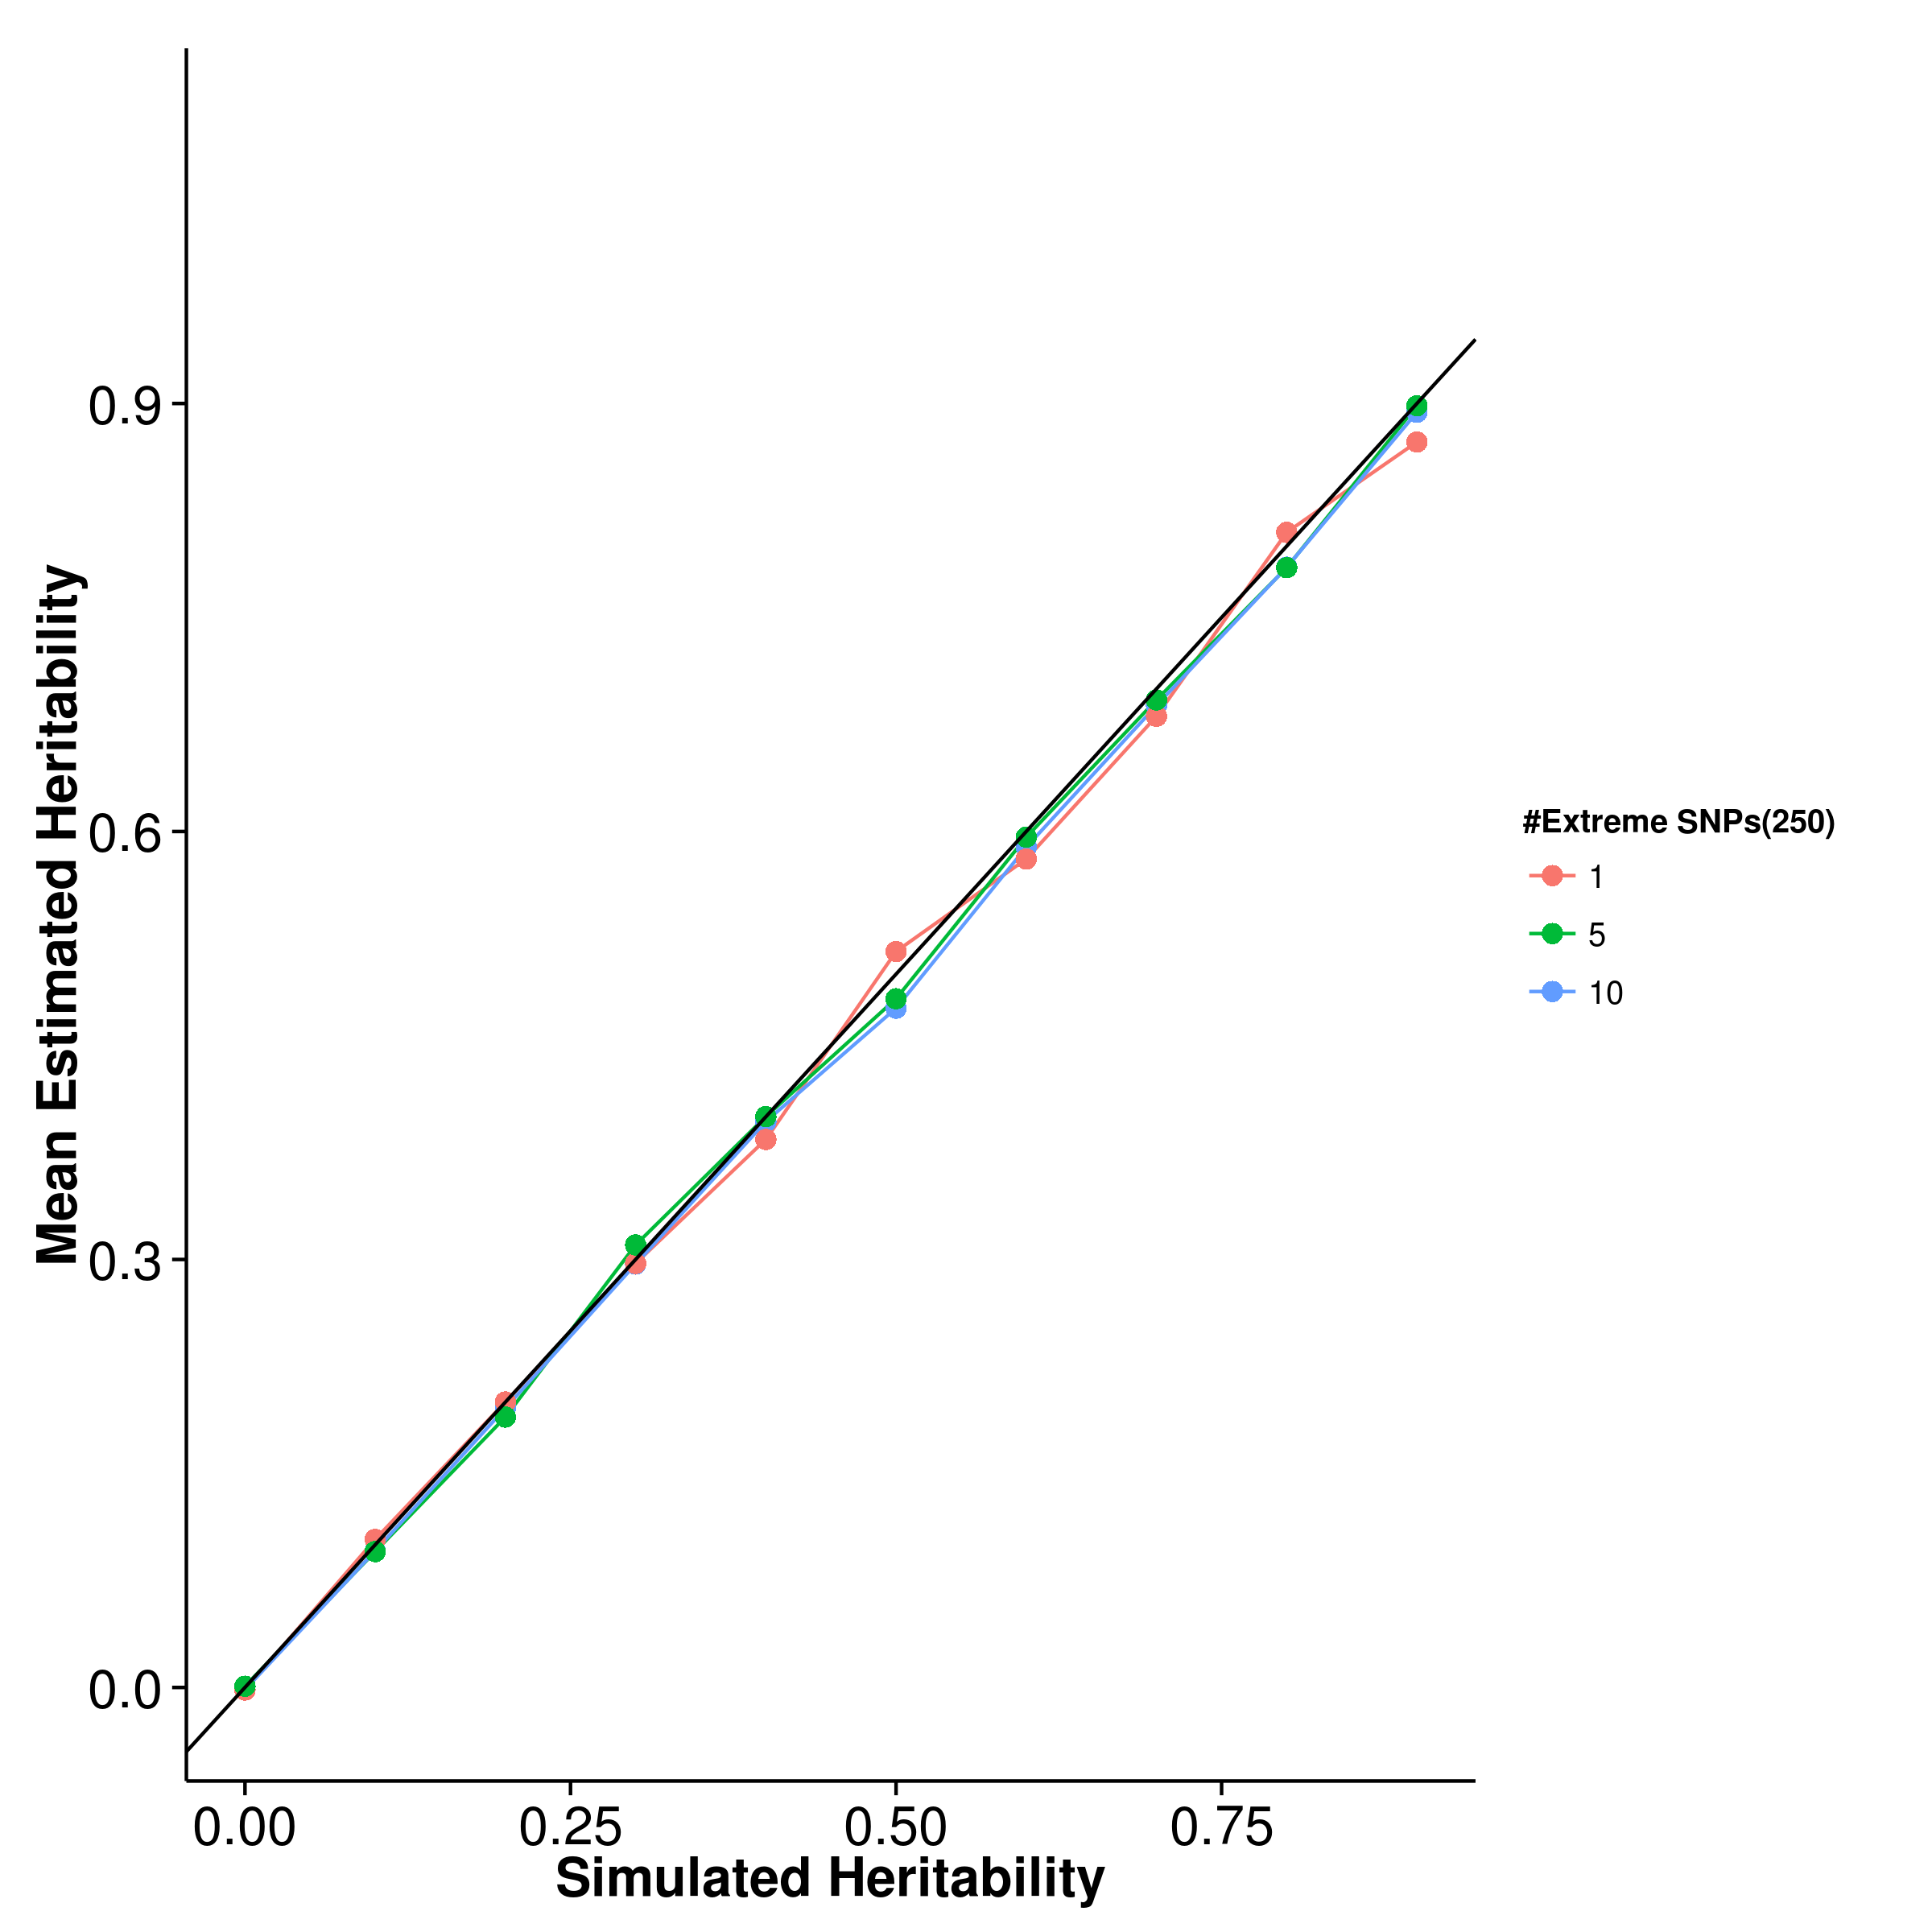
\includegraphics{figure/he_summary/extreme_250c/shrek_QtE_Extreme_mean.png}}
				\label{fig:shrekQtEx250cMean}
			}
			\subfloat[GCTA]{
				\scalebox{.4}{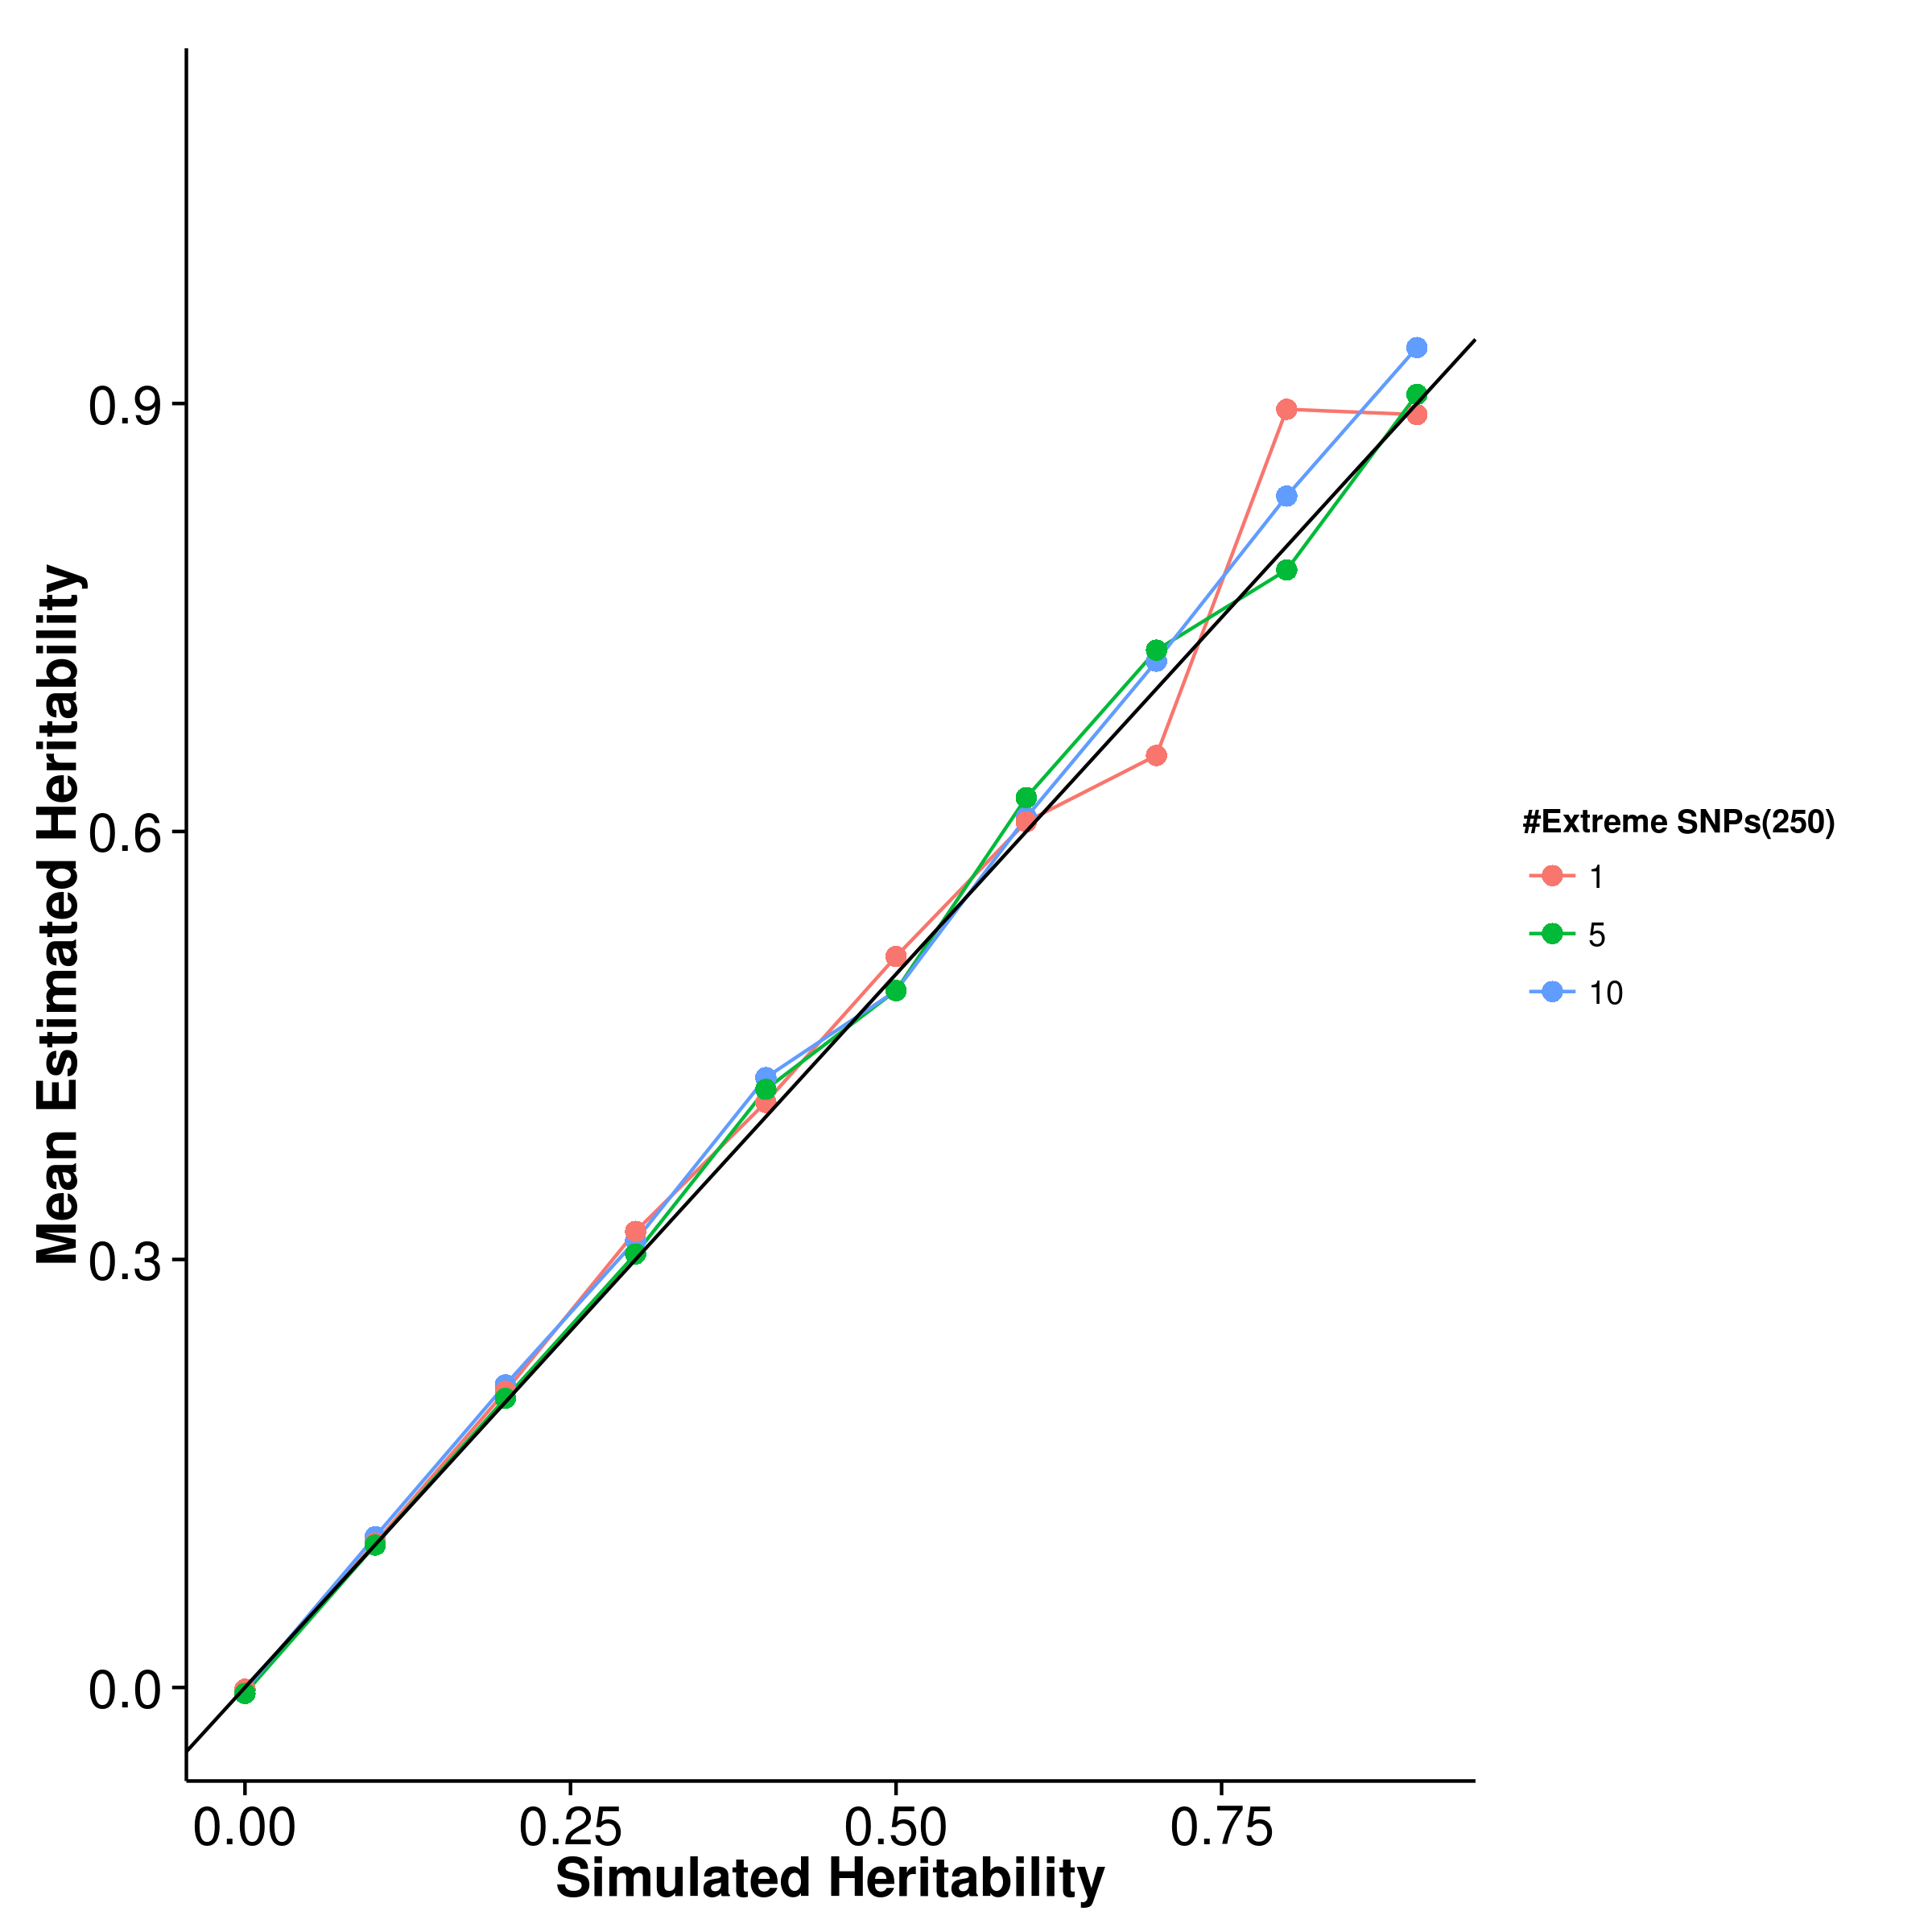
\includegraphics{figure/he_summary/extreme_250c/gcta_QtE_Extreme_mean.png}}
				\label{fig:gctaQtEx250cMean}
			}\\
			\subfloat[LDSC with fix intercept]{
				\scalebox{.4}{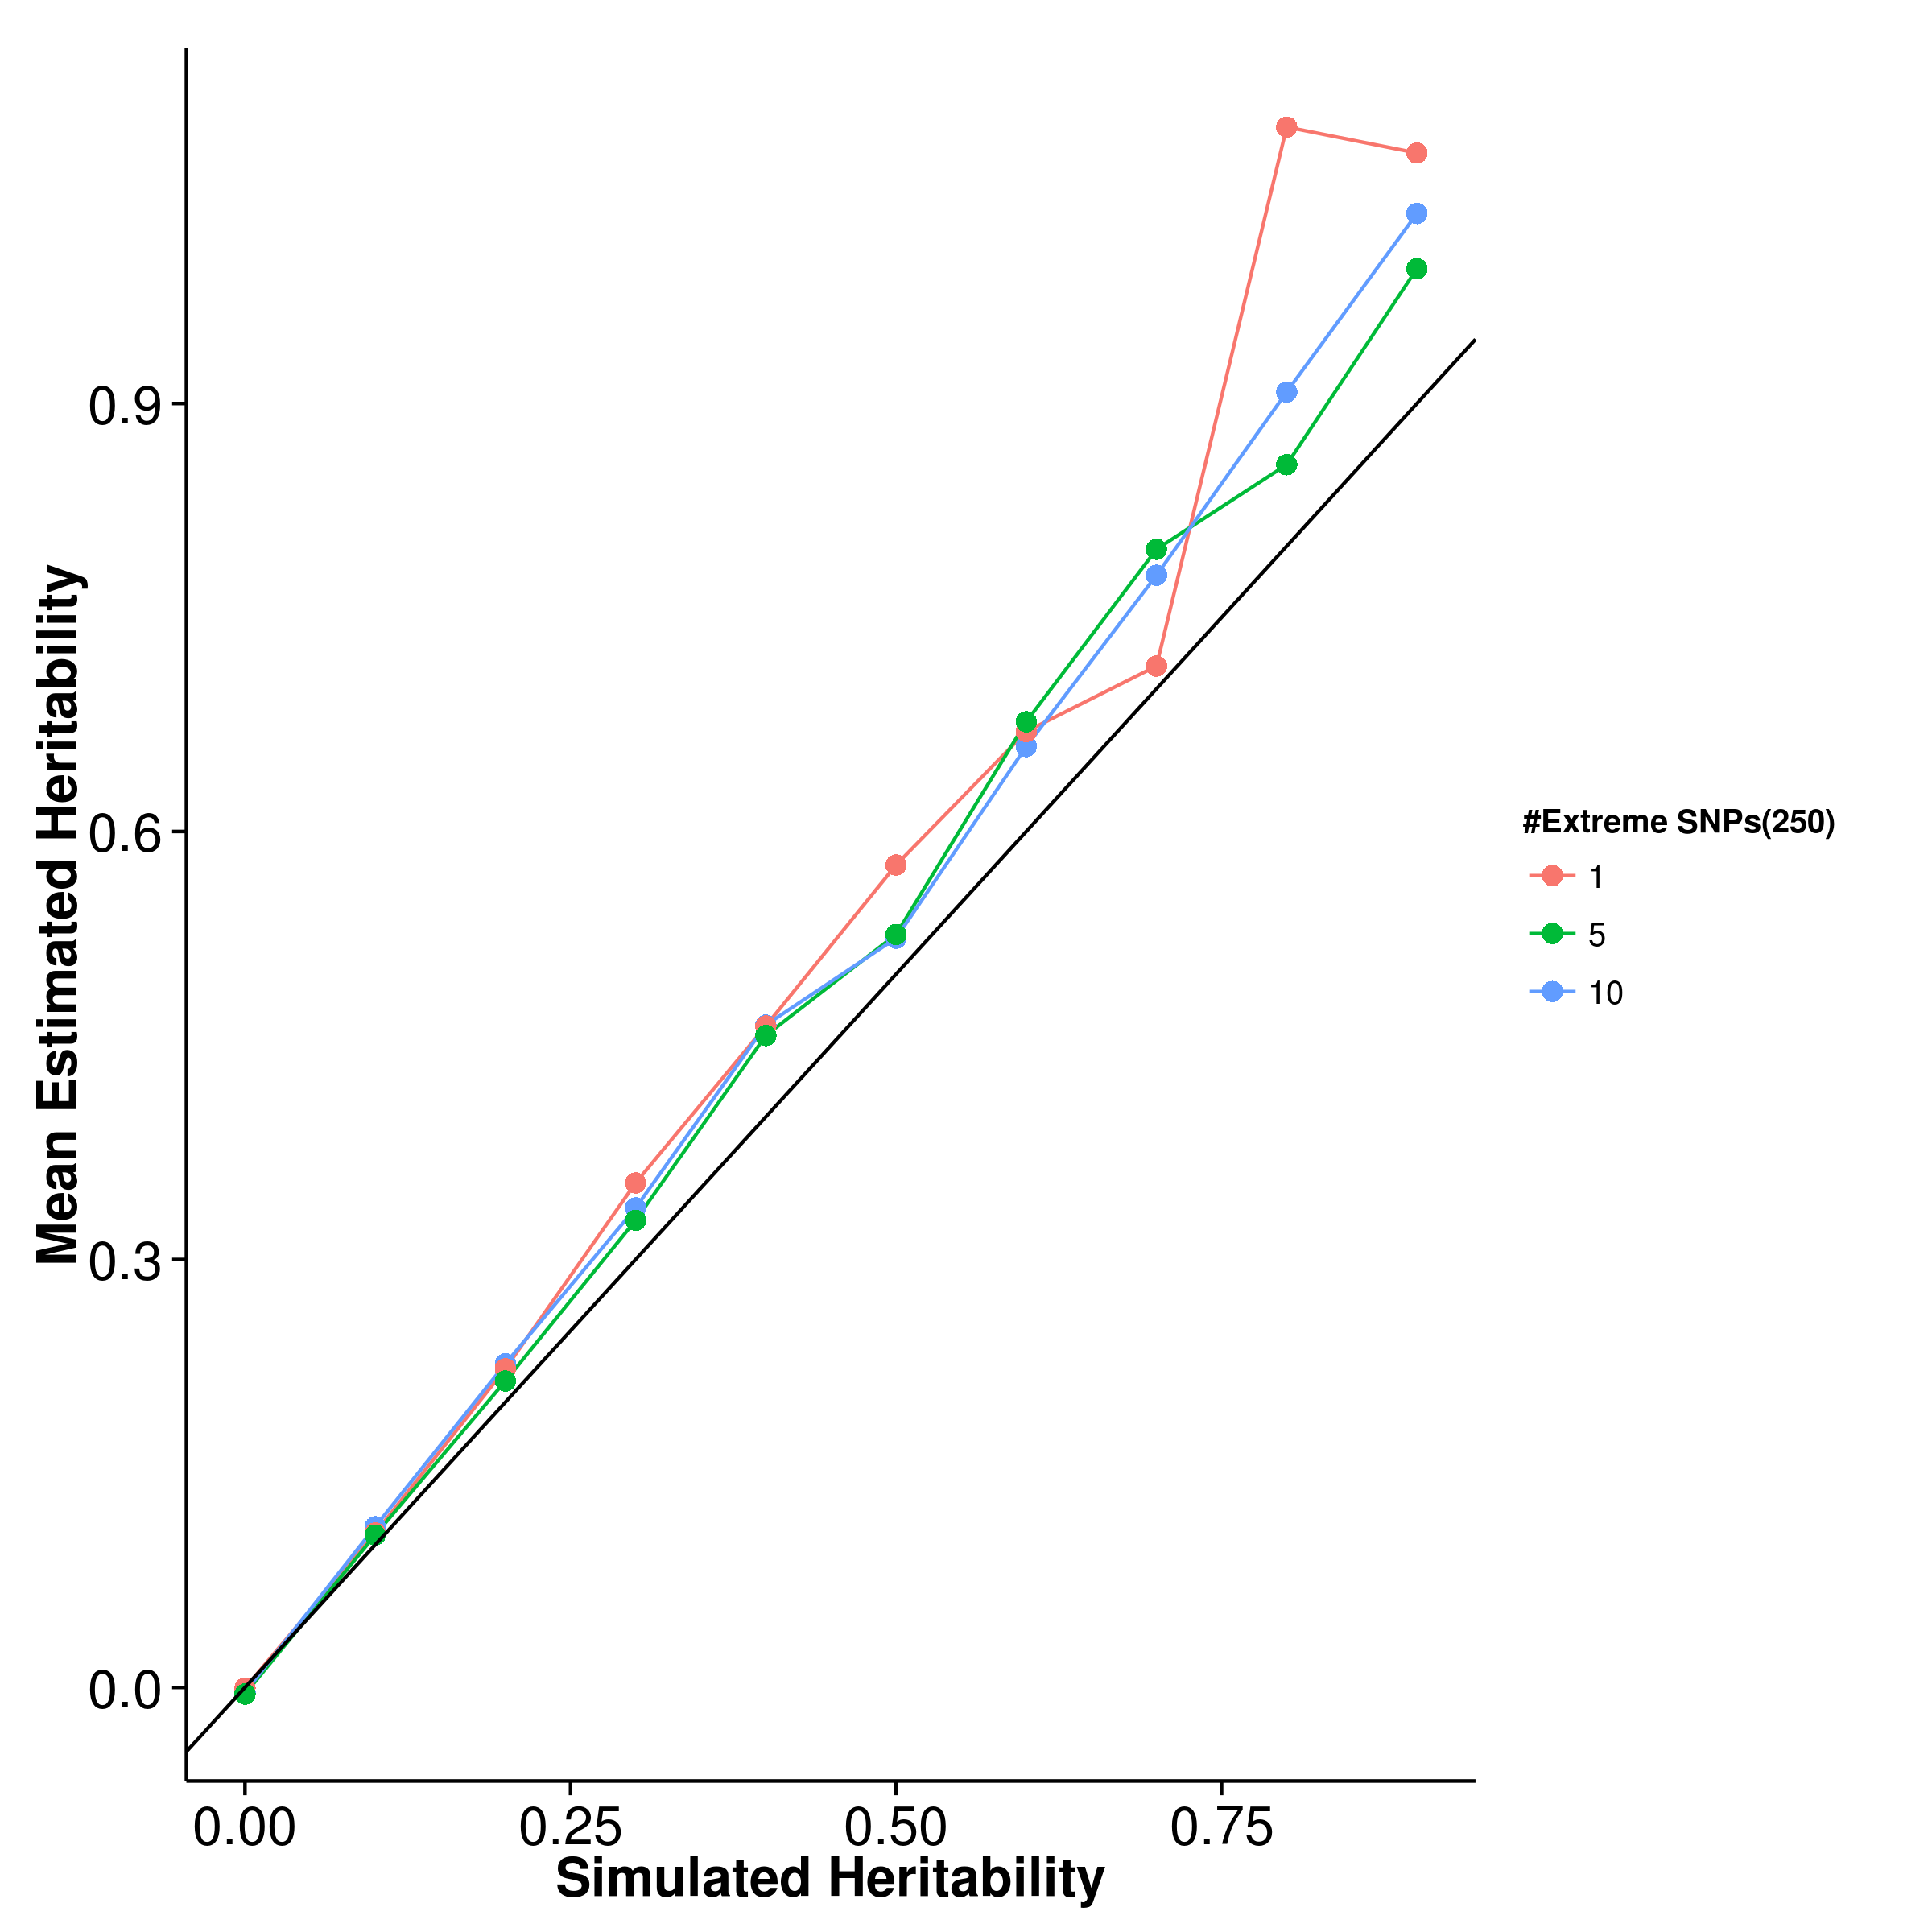
\includegraphics{figure/he_summary/extreme_250c/ldsc_QtE_Extreme_mean.png}}
				\label{fig:ldscQtEx250cMean}
			}
			\subfloat[LDSC with intercept estimation]{
				
				\scalebox{.4}{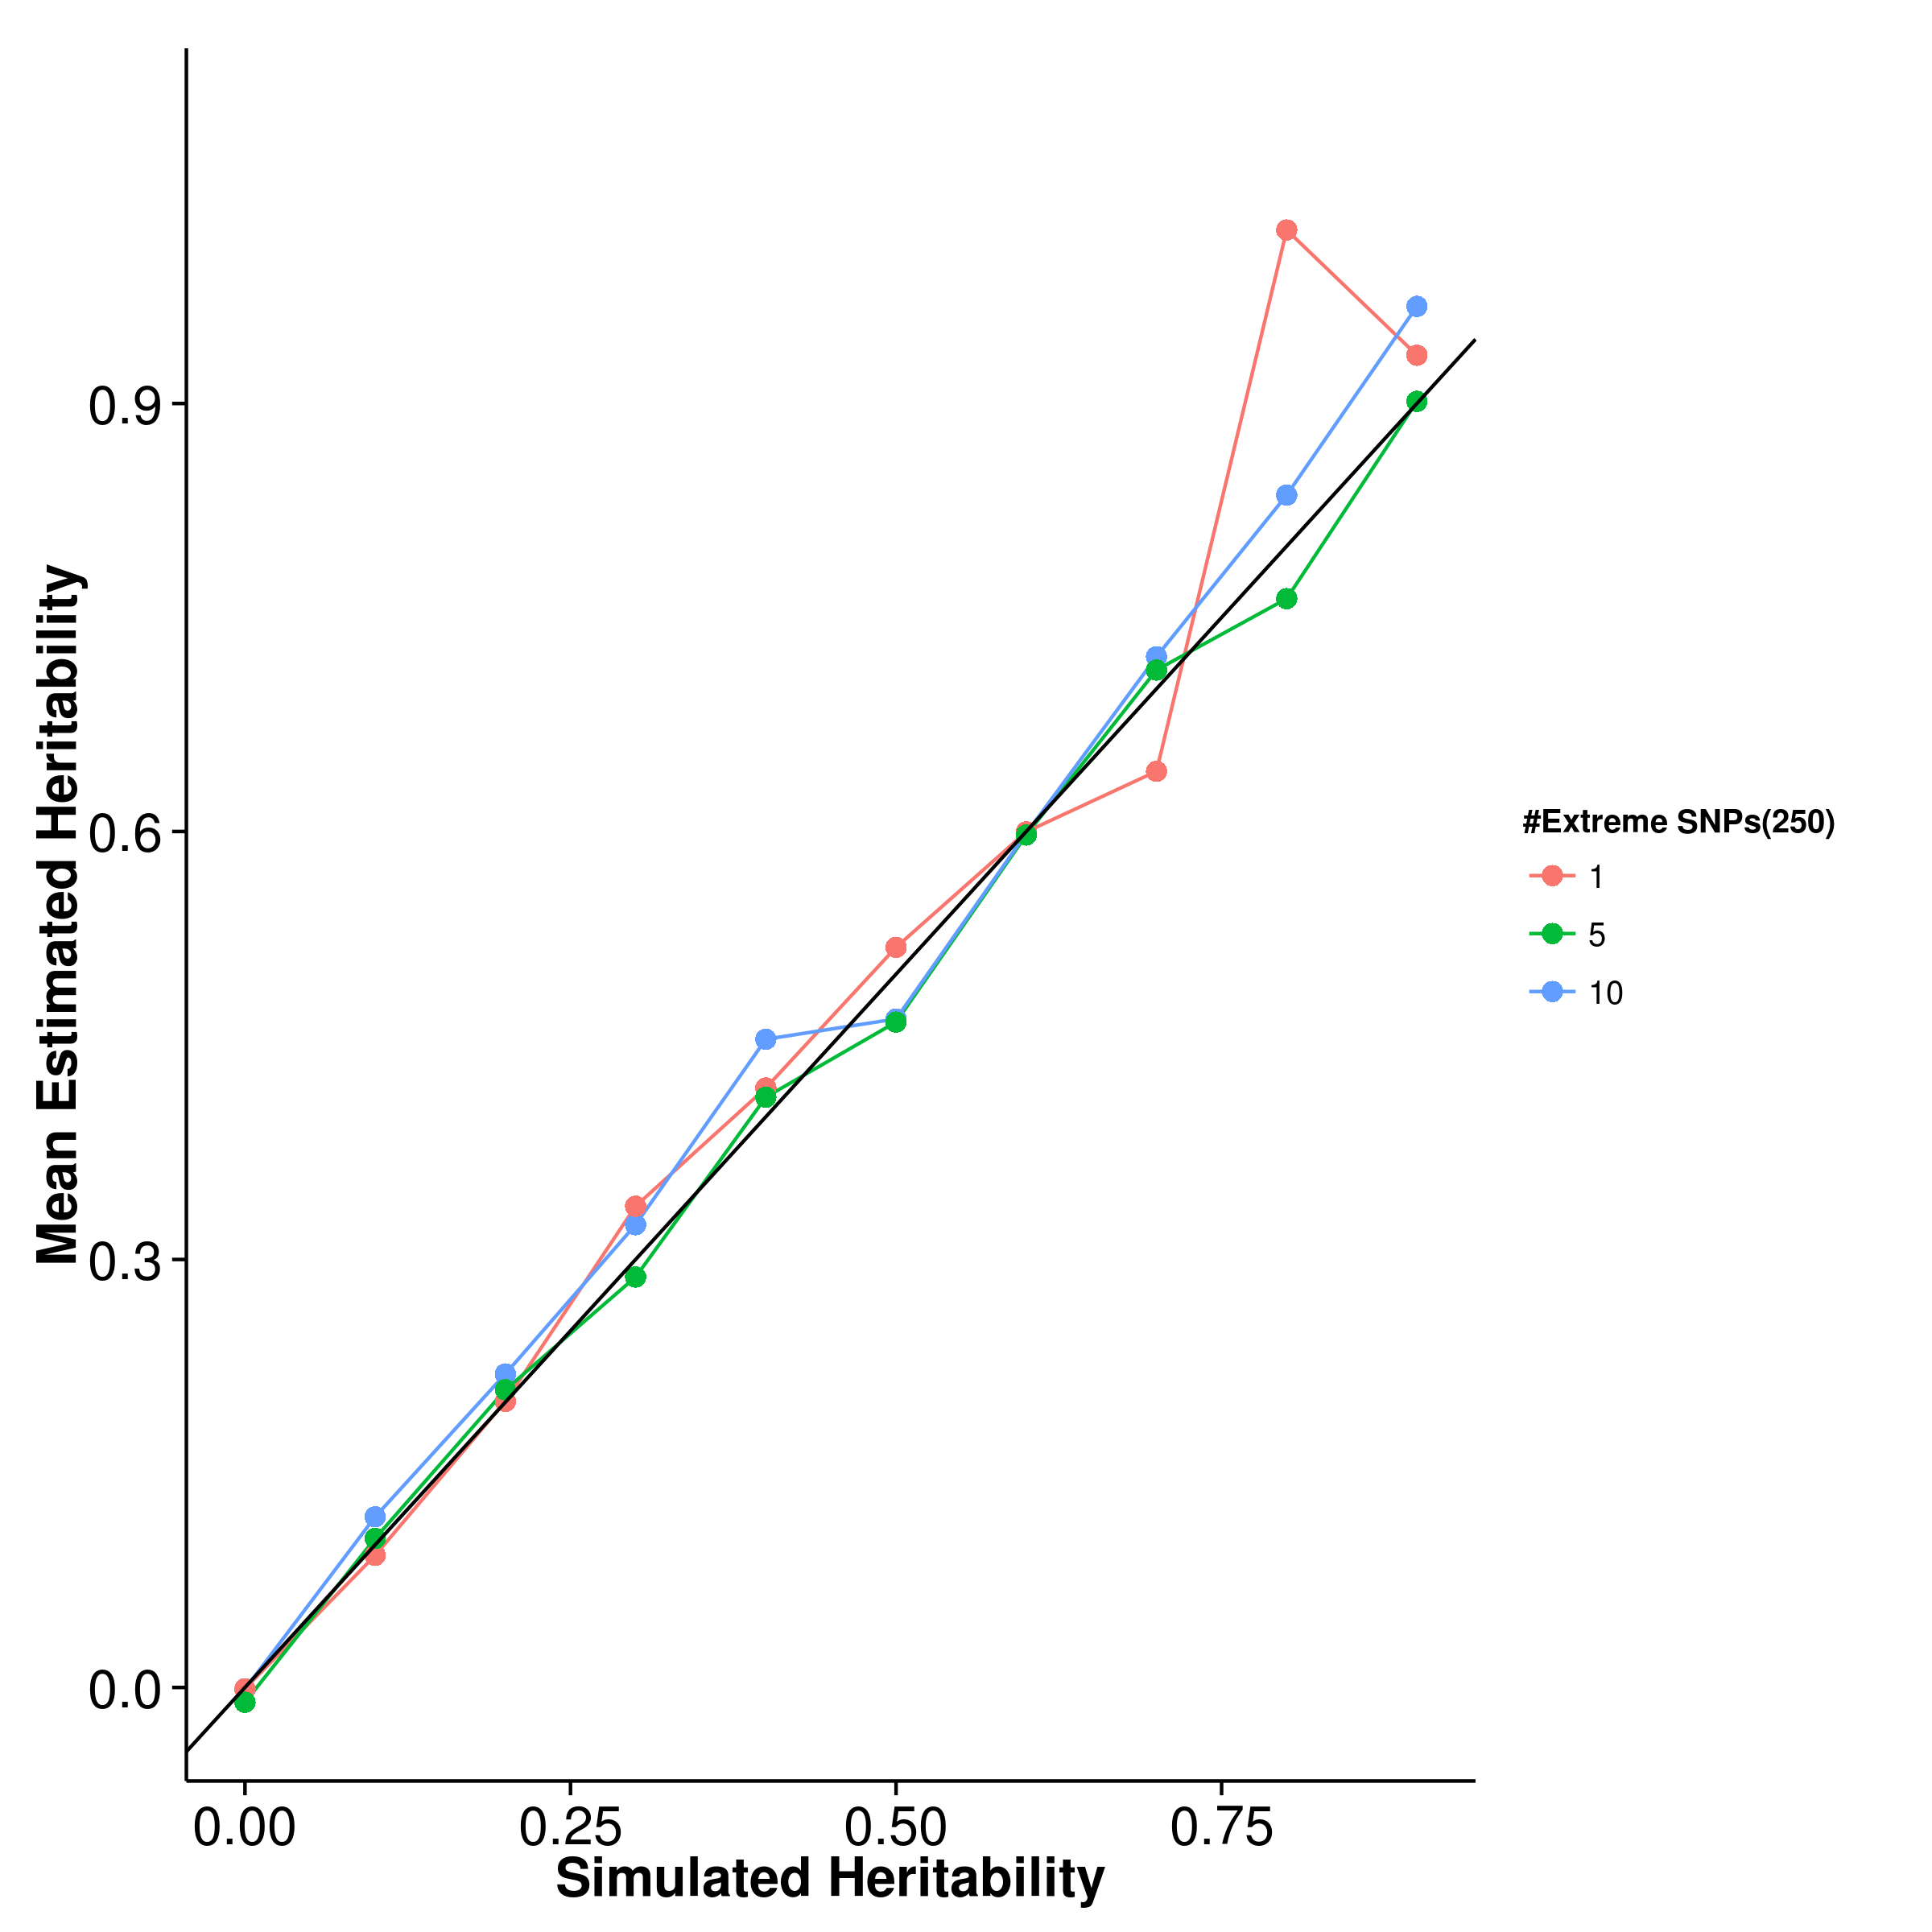
\includegraphics{figure/he_summary/extreme_250c/ldscIn_QtE_Extreme_mean.png}}
				\label{fig:ldscInQtEx250cMean}
			}
			\caption[Quantitative Trait with Extreme Effect Size Simulation Result(250 causal SNPs, Mean)]
			{Mean of results from quantitative trait simulation with extreme effect size simulation.
				250 causal \glspl{SNP} were simulated.
				It was observed that the mean estimation of heritability of all the tools were relatively unaffected by the number of \glspl{SNP} representing a large portion of effect, similar to what observed when 100 causal \glspl{SNP} were simulated.
				However, there seems to be an upward bias when \gls{ldsc} was performed with fixed intercept.
			} 
			\label{fig:QtEx250cMean}
		\end{figure}
		
		\begin{figure}
			\centering
			\subfloat[SHREK]{
				\scalebox{.4}{\includegraphics{figure/he_summary/extreme_250c/shrek_QtE_Extreme_sd.png}}
				\label{fig:shrekQtEx250cVar}
			}
			\subfloat[GCTA]{
				\scalebox{.4}{\includegraphics{figure/he_summary/extreme_250c/gcta_QtE_Extreme_sd.png}}
				\label{fig:gctaQtEx250cVar}
			}\\
			\subfloat[LDSC with fix intercept]{
				\scalebox{.4}{\includegraphics{figure/he_summary/extreme_250c/ldsc_QtE_Extreme_sd.png}}
				\label{fig:ldscQtEx250cVar}
			}
			\subfloat[LDSC with intercept estimation]{
				
				\scalebox{.4}{\includegraphics{figure/he_summary/extreme_250c/ldscIn_QtE_Extreme_sd.png}}
				\label{fig:ldscInQtEx250cVar}
			}
			\caption[Quantitative Trait with Extreme Effect Size Simulation Result(250 causal SNPs, Variance)]
			{Variance of results from quantitative trait simulation with extreme effect size simulation.
				250 causal \glspl{SNP} were simulated.
				Compared to the case where 100 causal \glspl{SNP} were simulated, most tools, except \gls{shrek} seems to be more sensitive to the number of \gls{SNP}(s) explaining large portion of effect, where a smaller number can lead to a higher variance.
			} 
			\label{fig:QtEx250cVar}
		\end{figure}
		
		\begin{figure}
			\centering
			\subfloat[SHREK]{
				\scalebox{.4}{\includegraphics{figure/he_summary/extreme_250c/shrek_QtE_Extreme_sdCom.png}}
				\label{fig:shrekQtEx250cVarCom}
			}
			\subfloat[GCTA]{
				\scalebox{.4}{\includegraphics{figure/he_summary/extreme_250c/gcta_QtE_Extreme_sdCom.png}}
				\label{fig:gctaQtEx250cVarCom}
			}\\
			\subfloat[LDSC with fix intercept]{
				\scalebox{.4}{\includegraphics{figure/he_summary/extreme_250c/ldsc_QtE_Extreme_sdCom.png}}
				\label{fig:ldscQtEx250cVarCom}
			}
			\subfloat[LDSC with intercept estimation]{
				
				\scalebox{.4}{\includegraphics{figure/he_summary/extreme_250c/ldscIn_QtE_Extreme_sdCom.png}}
				\label{fig:ldscInQtEx250cVarCom}
			}
			\caption[Quantitative Trait with Extreme Effect Size Simulation Result(250 causal SNPs, Estimated Variance)]
			{Estimated variance of results from quantitative trait simulation with extreme effect size simulation when compared to the empirical variance.
				250 causal \glspl{SNP} were simulated.
				The result of simulation were the same as the previous extreme effect simulation with 100 causal \glspl{SNP}.
			} 
			\label{fig:QtEx250cVarCom}
		\end{figure}
		% CC Rand Effect
		\subsection{Case Control Simulation}
		\begin{figure}
			\centering
			\subfloat[SHREK]{
				\scalebox{.4}{\includegraphics{figure/he_summary/cc_100c/shrek_CC_Random_mean.png}}
				\label{fig:shrekCCRandMean}
			}
			\subfloat[GCTA]{
				\scalebox{.4}{\includegraphics{figure/he_summary/cc_100c/gcta_CC_Random_mean.png}}
				\label{fig:gctaCCRandMean}
			}\\
			\subfloat[LDSC with fix intercept]{
				\scalebox{.4}{\includegraphics{figure/he_summary/cc_100c/ldsc_CC_Random_mean.png}}
				\label{fig:ldscCCRandMean}
			}
			\subfloat[LDSC with intercept estimation]{
				
				\scalebox{.4}{\includegraphics{figure/he_summary/cc_100c/ldscIn_CC_Random_mean.png}}
				\label{fig:ldscInCCRandMean}
			}
			\caption[Case Control with Random Effect Size Simulation Result(Mean)]
			{Mean of results from case control simulation with random effect size simulation.
				The performance of \gls{gcta} was as suggested by \citet{Golan2014} where there was an underestimation as prevalence decreases.
				On the other hand, \gls{ldsc} were upwardly biased when a fixed intercept was used and this bias was corrected when an estimation of intercept was allowed.
				\gls{shrek} does not seems to as sensitive to change in prevalence and the estimation were relatively robust.
				} 
			\label{fig:CCRandMean}
		\end{figure}
		
		\begin{figure}
			\centering
			\subfloat[SHREK]{
				\scalebox{.4}{\includegraphics{figure/he_summary/cc_100c/shrek_CC_Random_sd.png}}
				\label{fig:shrekCCRandVar}
			}
			\subfloat[GCTA]{
				\scalebox{.4}{\includegraphics{figure/he_summary/cc_100c/gcta_CC_Random_sd.png}}
				\label{fig:gctaCCRandVar}
			}\\
			\subfloat[LDSC with fix intercept]{
				\scalebox{.4}{\includegraphics{figure/he_summary/cc_100c/ldsc_CC_Random_sd.png}}
				\label{fig:ldscCCRandVar}
			}
			\subfloat[LDSC with intercept estimation]{
				
				\scalebox{.4}{\includegraphics{figure/he_summary/cc_100c/ldscIn_CC_Random_sd.png}}
				\label{fig:ldscInCCRandVar}
			}
			\caption[Case Control with Random Effect Size Simulation Result(Variance)]
			{Variance of results from case control simulation with random effect size simulation.
				It was clear that the prevalence affects the variance of estimation where a larger variance tends to increase the variance of estimation.
				Again, \gls{gcta} has the lowest variance, however, unlike in the quantitative trait simulation, \gls{shrek} has a lower average variance when compared to \gls{ldsc} with fixed intercept.
				Nonetheless, it was important to remember that in case control simulation, a much smaller amount of \glspl{SNP} was used, thus the results was not directly comparable to results from the quantitative simulation.
			} 
			\label{fig:CCRandVar}
		\end{figure}
		
		
		\begin{figure}
			\centering
			\subfloat[SHREK]{
				\scalebox{.4}{\includegraphics{figure/he_summary/cc_100c/shrek_CC_Random_sdCom.png}}
				\label{fig:shrekCCRandVarCom}
			}
			\subfloat[GCTA]{
				\scalebox{.4}{\includegraphics{figure/he_summary/cc_100c/gcta_CC_Random_sdCom.png}}
				\label{fig:gctaCCRandVarCom}
			}\\
			\subfloat[LDSC with fix intercept]{
				\scalebox{.4}{\includegraphics{figure/he_summary/cc_100c/ldsc_CC_Random_sdCom.png}}
				\label{fig:ldscCCRandVarCom}
			}
			\subfloat[LDSC with intercept estimation]{
				
				\scalebox{.4}{\includegraphics{figure/he_summary/cc_100c/ldscIn_CC_Random_sdCom.png}}
				\label{fig:ldscInCCRandVarCom}
			}
			\caption[Case Control with Random Effect Size Simulation Result(Estimated Variance)]
			{Estimated variance of results from case control simulation with random effect size simulation when compared to empirical variance.
				From the quantitative trait simulation with random effect size(\cref{fig:QtRandVarCom}), it was observed that the variance estimation of \gls{shrek} and \gls{gcta} were rater accurate.
				Similarly, in the case control simulation with 100 causal \glspl{SNP}, it was observed that the variance estimation of \gls{shrek} and \gls{gcta} were close to the empirical variance with slight bias.
				A large up-ward bias was observed for \gls{ldsc} with fixed intercept estimation but the bias was less when \gls{ldsc} was allowed to estimate the intercept.s
			} 
			\label{fig:CCRandVarCom}
		\end{figure}
		
		
		
		
	\section{Discussion}
	
	\section{Supplementary place holder}

	
	%Put these graphs in supplementary instead
	\chapter{Heritability of Schizophrenia}

\section{Introduction}
Apply Heritability estimation to the schizophrenia data.
The genetic correlation and partitioning of heritability
No one worked on linking schizophrenia with brain development directly?
% talk about the current research on schizophrenia?
% the overall heritablity estimation
% The genetic correlation done by the LDSC. 
% The theory of brain development 
% How the co-expression network works
% Drug response?
\section{Heritability Estimation}
This will be a very simple section, focused on how to perform the heritability estimation on \acrfull{scz}.
Should also tokenize the heritability into subcategories (e.g. immune, neuron, etc)
%Should not put too much weight into it, otherwise it will be a direct copy of LDSC. Won't really add much power. 


\subsection{Methodology}
\subsection{Result}
\section{Brain development and Schizophrenia}
\sectionmark{Brain development}
Here we will perform the WGCNA and brain development network.
Seeing how the whether if any brain development network were enriched with SNPs that explain the variance of phenotype
%Instead, we should put most focus here as no one has done it before
%Also descript brainspan here
\subsection{Methodology}
\subsubsection{Sample Quality Controls}
We obtain the developmental transcriptome data from BrainSpan (\url{http://www.brainspan.org/}). 
A total of 56 samples with different age were provided by BrainSpan with an average of 2.2 samples per age.

Studies suggested Hippocampus\citep{Velakoulis2006,Nugent2007}, Amygdala and Striatum\citep{Simpson2010} are brain regions involved in the etiology of schizophrenia. 
Therefore, we focus on building the gene co-expression network of hippocampus, amygdala and striatum in this study
It is worth noting that the Pre-frontal Cortex is also important for schizophrenia. 
However, as there isn't a well defined pre-frontal cortex samples from BrainSpan, we did not include the pre-frontal cortex in the current study.
RNA Sequencing data of the brain regions were obtained from BrainSpan and undergo a series of quality control before the construction of the network. 

For each sample age, when there are more than one samples, we select the sample with a dissection score $\ge3$ and an \gls{rin} $\ge7$. 
As some developmental stage only got 1 sample passing the quality check, we limit each developmental stage to have a maximum of 1 sample such that the final network will not be driven by a particular developmental stage. 
If multiple samples passed through the quality check threshold, we will prefer sample with higher dissection score. 
Shall multiple samples have the same dissection score, we will select the one with the highest \gls{rin}. 
And if the samples have the same dissection score and \gls{rin} value, we will randomly select one for the network construction.

After performing the quality control, a total of 16, 18 and 15 samples were selected for hippocampus, amygdala and striatum respectively.
The sample age ranged from \gls{gd}8 to 23 years old representing the fetal developmental stage till the age of onset of schizophrenia.

\subsubsection{Normalization of data}
The RNA Sequencing data were represented as \gls{rpkm} values. 
Genes with a low \gls{rpkm} can usually be a result from technical or biological noise\citep{Hart2013}.
To reduce noise in the final model, genes with a mean \gls{rpkm} $< 1$ in all samples were discarded. 
The \gls{rpkm} were then log transformed as instructed by the manual of \gls{wgcna}\citep{Langfelder2008}.

As there are insufficient samples for the construction of gene co-expression network for individual sample age, we try to construct networks with genes co-expressed through all sample stage. 
This is achieved by taking the standardized log$_2$ \gls{rpkm} across sample age such that all genes has a mean of 0 and standard deviation of 1.

At the end, there were 17,168 genes, 17,038 genes and 17,166 genes passing through the quality threshold and were used for the construction of co-expression network in hippocampus, amygdala and striatum respectively. 

\subsubsection{Network Construction}
\gls{wgcna} (ver 1.47) were used for the construction of gene co-expression network\citep{Langfelder2008}. 
The \emph{blockwiseModules} function, using Biweight Midcorrelation for the construction of correlation matrix and a restriction of minimum network size of 30. 
For the construction of gene co-expression networks in hippocampus, the soft-power threshold were set to 15 where it is the first threshold value which has $R^2 > 0.8$ (0.817) and the $R^2$ is saturated\citep{Zhang2005}.%(\cref{fig:softpowerThreshold})
As for striatum, the soft-power threshold were set to 20. 
Again, this is the first threshold value with $R^2 >0.8$ (0.879) and where the $R^2$ is saturated.

On the other hand, for amygdala, soft-power threshold were set to 9 which is the first threshold for $R^2$ to reach saturation. 
However, with a soft-power threshold of 9, the $R^2$ were only 0.776, which is lower than the recommended 0.8 threshold.
The reason behind this decision was that the first soft-power threshold to have $R^2 > 0.8$ is 30.
Under this threshold, the mean connectivity of the resulting networks will be around 23.6 with a median connectivity of 2.51.
Such level of connectivity will likely yield networks that are too small to useful.
If one would like to satisfy both requirement of threshold selection, a threshold $>30$ are likely required and any networks constructed will likely to be small.
As a result of that, we select threshold of 9 where networks with reasonable size can be constructed.

%\begin{figure}
%	\caption[Soft-power threshold selection]{Soft-power threshold selection. A soft-power of 13 were selected as it is the first threshold value having $R^2 > 0.8$ (0.817) and where the $R^2$ is saturated.}
%	\centering
%	\scalebox{.8}{\includegraphics{figure/SoftpowerThreshold.png}}
%	\label{fig:softpowerThreshold}
%\end{figure}

\subsubsection{Expression correlation with Age}
The co-expression network constructed with the standardized gene expression value will contains genes that co-express in all sample age.
However, this does not necessary suggest the expression of these genes are correlated with the sample age.
To identify gene co-expression networks with expressions correlated with the sample age, we performed a correlation analysis between the module eigen-genes and the sample age. 
Network eigen-genes were calculated as the first \gls{pc} of expressions of the genes within individual networks using the \emph{moduleEigengenes} function from \gls{wgcna}. 
Age were represented as month from conception such that 8 post-conception week will be represented as 2; 4 months will be represented as 10 and 12 years will be represented as 154 etc. 
Finally, correlation between age and network eigen-gene expression were calculated pearson correlation.

\subsubsection{Functional Annotation}
\gls{GO} based enrichment analysis of the significant module was performed using GOrilla\citep{Eden2009}.
Genes within the networks were provide as the target gene lists and all the genes passed quality controls were used as the background gene list.
As \gls{GO} terms tends to be redundant and overlaps with each other, it will aid the interpretation of \gls{GO} results based by clustering and reducing the \gls{GO} terms based on their similarity. 
Thus, \gls{GO} enrichment results were summerized by REViGO\citep{Supek2011} and significant representative \gls{GO} terms were obtained.

\subsubsection{Associate Co-expression network with \glsentryshort{pgc} schizophrenia data}
The co-expression networks were built from normal samples and should not be representative of the brain expression pattern in schizophrenia patients.
it is however interesting to see if the co-expression networks were disrupted in schizophrenia patient.
To test whether if the gene co-expression networks contain genes that are jointly associated with schizophrenia, we first use \gls{MAGMA}\citep{DeLeeuw2015}(version v1.03) to compute the gene-base p-value from the \gls{SNP} wise p-value obtained from \gls{pgc}. 
Gene-set enrichment analysis were then performed on networks that were significantly correlated with developmental age. 
As we were only interested in whether if the genes within the networks were jointly associated with schizophrenia, we only focus on the result of the self-contained gene set analysis and ignore the result from competitive analysis.

\subsubsection{Partitioning of Heritability}

\subsection{Result}
\subsubsection{Co-Expression Network}
A total of 35 networks were constructed based on the hippocampus samples with a mean network size of 421.6.
On the other hand, 28 networks were constructed for amygdala with mean network size of 591.86.
Finally, 25 networks with mean size of 494.52 were constructed from the striatum samples.

Of the all the networks constructed, only one network from hippocampus(\cref{tab:hipModSig}) and three networks from amygdala(\cref{tab:amyModSig}) were significantly correlated with sample age after bonferroni correction threshold (p-value $<0.00143$ for hippocampus, p-value $<0.00179$ for amygdala and p-value $<0.002$ for striatum) .
\begin{table}
	\centering
	\caption[Correlation of sample age with the module eigen gene]{Correlation of sample age with the module eigen gene. 
		Module eigen-gene was defined as the first \gls{pc} of genes within the module. 
		After correcting for multiple testing, only the black module was considered as significantly correlated with the sample age.}
	\subfloat[Hippocampus]{
		\begin{tabular}{rrr}
			\toprule
			& Correlation & Pvalue \\
			\midrule
			black & 0.804653 & 0.000171 \\
			blue  & -0.61648 & 0.010981 \\
			red   & -0.60207 & 0.013595 \\
			darkred & -0.59137 & 0.015833 \\
			greenyellow & -0.56995 & 0.021168 \\
			yellow & 0.567828 & 0.021763 \\
			darkgrey & -0.55246 & 0.026474 \\
			saddlebrown & -0.52983 & 0.034783 \\
			turquoise & -0.51371 & 0.041809 \\
			purple & -0.46788 & 0.067606 \\
			darkolivegreen & -0.41272 & 0.112122 \\
			sienna3 & -0.39535 & 0.129604 \\
			darkturquoise & 0.386541 & 0.139154 \\
			darkorange & 0.384966 & 0.140912 \\
			darkmagenta & 0.375586 & 0.151688 \\
			brown & 0.366095 & 0.163144 \\
			tan   & -0.36522 & 0.164229 \\
			pink  & 0.348979 & 0.18524 \\
			magenta & -0.32559 & 0.218473 \\
			midnightblue & -0.29168 & 0.273014 \\
			lightgreen & 0.289921 & 0.276056 \\
			paleturquoise & -0.28045 & 0.29276 \\
			white & 0.27727 & 0.29849 \\
			orange & 0.19607 & 0.466754 \\
			steelblue & 0.17355 & 0.520357 \\
			skyblue & 0.145869 & 0.589857 \\
			lightyellow & -0.11665 & 0.667028 \\
			green & -0.09882 & 0.715786 \\
			violet & -0.08757 & 0.747076 \\
			lightcyan & -0.0656 & 0.809257 \\
			cyan  & -0.06441 & 0.812661 \\
			darkgreen & -0.03914 & 0.885582 \\
			salmon & 0.038727 & 0.886769 \\
			royalblue & -0.03785 & 0.889314 \\
			grey60 & 0.03119 & 0.908709 \\
			\bottomrule
			\label{tab:hipModSig}%
		\end{tabular}%
	}
	\qquad%
	\subfloat[Amygdala]{
		\begin{tabular}{rrr}
			\toprule
			& Correlation & P-value \\
			\midrule
			tan   & 0.849999 & $7.96\times 10^{-6}$ \\
			yellow & -0.757 & $2.76\times 10^{-4}$ \\
			pink  & -0.68541 & $1.69\times 10^{-3}$ \\
			greenyellow & -0.67831 & $1.97\times 10^{-3}$ \\
			red   & -0.64532 & $3.83\times 10^{-3}$ \\
			turquoise & -0.59771 & $8.80\times 10^{-3}$ \\
			lightyellow & -0.56347 & 0.0149 \\
			brown & 0.548516 & 0.0184 \\
			darkgreen & -0.46366 & 0.0526 \\
			blue  & -0.4604 & 0.0545 \\
			purple & -0.44182 & 0.0664 \\
			darkgrey & -0.39065 & 0.109 \\
			orange & -0.36966 & 0.131 \\
			white & 0.28737 & 0.248 \\
			darkred & 0.283247 & 0.255 \\
			black & 0.271383 & 0.276 \\
			salmon & -0.24203 & 0.333 \\
			skyblue & 0.207071 & 0.410 \\
			cyan  & 0.18778 & 0.456 \\
			lightgreen & 0.166495 & 0.509 \\
			grey60 & 0.15156 & 0.548 \\
			midnightblue & 0.136078 & 0.590 \\
			magenta & -0.13459 & 0.594 \\
			darkturquoise & 0.129954 & 0.607 \\
			lightcyan & 0.090241 & 0.722 \\
			darkorange & -0.05166 & 0.839 \\
			green & -0.04745 & 0.852 \\
			royalblue & 0.020456 & 0.936 \\
			\bottomrule
			\label{tab:amyModSig}%
		\end{tabular}%
	}
\end{table}

By plotting the mean expression of each network against the sample age, one can inspect how the dynamic of the network changes across different developmental stage.
Thus, mean expression of all the genes within the significant networks were calculated for all amygdala (n=33) and hippocampus (n=32) samples from BrainSpan.
The mean \gls{rpkm} values were then log$_2$ transformed and plot against the sample age where a line of bests fit was calculated using the \emph{stat\_smooth} with the loess function from R package \emph{ggplot2}(version 1.0.1). (\cref{fig:allMod}).

The expression pattern observed were intriguing where there both the ``black''(\cref{fig:blackMod}) and ``tan'' (\cref{fig:tanMod}) networks have mean gene expression level increase as development progress and reaches its peak at around late adolescence ($\approx 18-21$), concurring with the onset age of schizophrenia.
Similarly, an inverse pattern were observed with the ``yellow'' network where its mean expression was highest during fetal development and drop steadily to its lowest around late adolescence and increase again afterwards(\cref{fig:yellowMod}).

The expression pattern of the ``black'' and ``tan'' networks are of particular interest as they follow the inverted ``U'' shape trajectory of the grey matter volumn observed in previous studies\citep{Gogtay2011}, suggest that they might have a role in mediating brain development. 
\begin{figure}
	\caption[Mean Gene Expression across developmental age]{Mean Gene Experssion across developmental age.
		Mean \gls{rpkm} values of genes in the significant modules were plot with respect to the sample age.
		A loess smoothing curve was also plotted. 
		%Might want to talk somemore about it
	}
	\centering
	\subfloat[``Black'' Network from Hippocampus]{
		\scalebox{.4}{\includegraphics{figure/network/hip_network.png}}
		\label{fig:blackMod}
	}
	\subfloat[``Tan'' Network from Amygdala]{
		\scalebox{.4}{\includegraphics{figure/network/amy_tan_network}}
		\label{fig:tanMod}
	}\\
	\subfloat[``Pink'' Network from Amygdala]{
		\scalebox{.4}{\includegraphics{figure/network/amy_pink_network}}
		\label{fig:pinkMod}
	}
	\subfloat[``Yellow'' Network from Amygdala]{
		\scalebox{.4}{\includegraphics{figure/network/amy_yellow_network}}
		\label{fig:yellowMod}
	}
	\label{fig:allMod}
\end{figure}



\subsubsection{Functional Annotation}
Upon performing the \gls{GO} enrichment analysis, a total of 16 \gls{GO} terms were enriched in the ``black'' hippocampus network, 4 in the ``tan'' amygdala network and 45 in the ``yellow'' amygdala network. 
No \gls{GO} term was enriched in the ``pink'' amygdala network.

The enriched \gls{GO} terms of the ``yellow'' amygdala network were mainly related to translation and transcription and were not specific to brain function or development(\cref{tab:yellowGO}). 
On the contrary, the \gls{GO} terms enriched in the ``black'' hippocampus network were highly relevant to brain function and development (\cref{tab:blackGO})(e.g. ``central nervous system development'' and ``glutamate metabolic process'') and the ``tan'' amygdala network were also related to ammonium ion metabolism (\cref{tab:tanGO}) which is vita for glutamine synthesis from glutamate\citep{Liaw1995}. 

Together, it is highly likely that the ``black'' hippocampus and ``tan'' amygdala networks are related to brain development and function.

\begin{table}[h]
	\centering
	\caption[\glsentryshort{GO} enrichment results for the ``black'' network from Hippocampus]{\gls{GO} enrichment results for the ``black'' network from Hippocampus.
		Among the enriched \gls{GO} terms, it was most interesting to identify a number of brain developmental related \gls{GO} terms such as ``central nervous system development'', ``axon ensheathment in central nervous system'', ``glutamate metabolic process'' and ``positive regulation of gliogenesis''. 
		Surprisingly, \gls{GO} related to immune systems were also observed ``positive regulation of production of molecular mediator of immune response''.
	}
	\begin{tabular}{rrr}
		\toprule
		term\_ID & description & p-value \\
		\midrule
		GO:0019752 & carboxylic acid metabolic process & $4.92\times 10^{-6}$ \\
		GO:0007417 & central nervous system development & $5.94\times 10^{-5}$ \\
		GO:0002821 & positive regulation of adaptive immune response & $6.12\times 10^{-5}$ \\
		GO:0006082 & organic acid metabolic process & $1.03\times 10^{-3}$ \\
		GO:0032291 & axon ensheathment in central nervous system & $1.86\times 10^{-3}$ \\
		GO:1901565 & organonitrogen compound catabolic process & $1.99\times 10^{-3}$ \\
		GO:0006536 & glutamate metabolic process & $3.54\times 10^{-3}$ \\
		GO:0021762 & substantia nigra development & $3.73\times 10^{-3}$ \\
		GO:0044281 & small molecule metabolic process & $4.34\times 10^{-3}$ \\
		GO:0030194 & positive regulation of blood coagulation & $4.59\times 10^{-3}$ \\
		GO:0009607 & response to biotic stimulus & $6.14\times 10^{-3}$ \\
		GO:0002702 & positive regulation of production of molecular mediator of immune response & $6.21\times 10^{-3}$ \\
		GO:0034103 & regulation of tissue remodeling & $6.21\times 10^{-3}$ \\
		GO:0014015 & positive regulation of gliogenesis & $7.47\times 10^{-3}$ \\
		GO:0098542 & defense response to other organism & $7.95\times 10^{-3}$ \\
		GO:0019835 & cytolysis & $8.72\times 10^{-3}$ \\
		\bottomrule
	\end{tabular}%
	\label{tab:blackGO}%
\end{table}%
\begin{table}[h]
	\centering
	\caption[\glsentryshort{GO} enrichment results for the ``tan'' network from Amygdala]{\gls{GO} enrichment results for the ``tan'' network from Amygdala.
		Unlike the ``black'' network, only a small number of \gls{GO} terms were enriched. 
		However, these \gls{GO} terms are relatively specific to amine/ammonium ion metabolism.
		Interestingly, ammonium ion are essential to the synthesis of glutamine from glutamate, suggesting that this network might be relate to the glutamate system.
	}
	\begin{tabular}{rrr}
		\toprule
		term\_ID & description & p-value \\
		\midrule
		GO:0097164 & ammonium ion metabolic process & $1.37\times 10^{-3}$ \\
		GO:0044106 & cellular amine metabolic process & $4.2\times 10^{-3}$ \\
		GO:0009308 & amine metabolic process & $5.41\times 10^{-3}$ \\
		GO:0046519 & sphingoid metabolic process & $6.01\times 10^{-3}$ \\
		\bottomrule
	\end{tabular}%
	\label{tab:tanGO}%
\end{table}%

\subsubsection{Associate Co-expression network with \glsentryshort{pgc} schizophrenia data}
Although the co-expression network were extremely interesting for their expression pattern and functional enrichment in brain development and function related \gls{GO} terms, there were no evidence of their involvement nor importance in schizophrenia.
Therefore it is of particular interest for us to test whether if genes within these co-expression networks were associated withs schizophrenia. 

First, gene base p-value of 18,622 genes were calculated using p-values from the \gls{pgc} schizophrenia working group\citep{Ripke2014}.
Gene set enrichment analysis were then performed using \gls{MAGMA}\citep{DeLeeuw2015} to test whether if there genes within the ``black'' hippocampus and ``tan'' amygdala networks were significantly associated with schizophrenia.

Based on the self-contained gene set enrichment analysis, genes within both networks were significantly associated with schizophrenia with p-value of $1.38\times 10^{-41}$ for the ``tan'' amygdala network and $2.70\times 10{-74}$ for the ``black'' hippocampus network.
These suggest that these networks might be disrupted in schizophrenia patients.
%Network	Size	self-contained	competitive
%Amygdala        289   1.3869e-41      0.44715
%Hippocampus     458   2.6993e-74      0.20002




\subsubsection{Partitioning of Heritability}

\section{Discussion}
	
	\chapter{Heritability of Response to antipsychotic treatment}
	\chaptermark{Response to antipsychotic treatment}
	%Maybe a section instead of a chapter?
	One of the aim of pharmacogenetics is to be able to predict the treatment response of individuals based on their genetic data.
	An important parameter to consider here will be the heritability of antipsychotic drug response for it provide an upper bound of how much of the variation in treatment response can be predicted by genetic data. 
	However, it was extremely difficult to obtain twins and family data on antipsychotic drug response, making it impossible for the estimation of the heritability.
	
	In this chapter, we aimed to estimate the heritability of antipsychotic response, using data from the antipsychotic \gls{GWAS} and Exome Sequencing study. 
	Moreover, we were interested in investigating which functional categories were more important in antipsychotic drug response. 
	Therefore, we will also perform the partitioning of heritability on a series of functional categories.
	
	\section{Introduction}
	Here we try to use Beatrice's data and estimate the heritability explained in drug response.
	Should also repeat the region-wise heritability
	\section{Methodology}
	\section{Result}
	\section{Discussion}

	\chapter{Conclusion}
	
	
	
	
	
	
	
	
	\backmatter
	\printbibliography[heading=bibintoc,title={Bibliography}]
	\chapter*{Supplementary Materials}
	\beginsupplement
	\chapter*{Appendix}

\end{document}


